\documentclass{wissdoc}

% ----------------------------------------------------------------
%    My Information
% ----------------------------------------------------------------

\newcommand{\myname}{Lucas~Czech}
\newcommand{\mycity}{Neuss}
% \newcommand{\mytitle}{Novel Methods for Post-Processing Evolutionary Data Using Machine Learning Techniques}
\newcommand{\mytitle}{Novel Methods for\\Analyzing and Visualizing\\Phylogenetic Placements}
% \newcommand{\myinstitute}{Institute for Program Structures\\and Data Organization (IPD)}

\newcommand{\reviewerone}{Prof.~Dr.~Alexandros~Stamatakis}
\newcommand{\reviewertwo}{Prof.~Dr.~Emmanuel~Müller}
\newcommand{\advisorone}{}
\newcommand{\advisortwo}{}

\newcommand{\timestart}{July 1, 2014}
\newcommand{\timeend}{June 30, 2019}
\newcommand{\submissiontime}{June 30, 2019}
\newcommand{\submissionlocation}{Karlsruhe}

\author{\myname}
\title{\mytitle}

%% Informationen für die PDF-Datei
\pdfstringdefDisableCommands{\def\\#1{ #1}}
\hypersetup{
	pdfauthor={\myname},
	pdftitle={\mytitle},
	pdfsubject={In this work, we present novel methods to analyze, visualize, and cluster phylogenetic placement data of large-scale environmental metagenomic sequence samples.},
	pdfkeywords={Computational Phylogenetics, Phylogenetic Trees, Phylogenetic Placement, Data Analysis, Data Visualization, Clustering, Computational Biology, Bioinformatics, Software Development}
}

% ----------------------------------------------------------------
%    Settings
% ----------------------------------------------------------------

% ------------------------------------------
%  Text editing
% ------------------------------------------

\newcommand\todo[1]{{\color{purple}{TODO: #1}}}

% ------------------------------------------
%  Custom styles
% ------------------------------------------

\newcommand\toolname{\textsc}
\newcommand\taxonname{\textit}
\newcommand\fileformat{\texttt}
\newcommand\nucleobase[1]{\texttt{#1}}

% Epigraph
% https://tex.stackexchange.com/questions/193178/specific-epigraph-style
\usepackage{epigraph}
\setlength\epigraphwidth{.8\textwidth}
\setlength\epigraphrule{0pt}

% ------------------------------------------
%  References
% ------------------------------------------

\newcommand\secref[1]{Section~\ref{#1}}
\newcommand\figref[1]{Figure~\ref{#1}}
% \newcommand\suppfigref[1]{S\ref{#1}~Fig}
\newcommand\tabref[1]{Table~\ref{#1}}
\renewcommand\algref[1]{Algorithm~\ref{#1}}
\newcommand\eqnref[1]{Equation~\ref{#1}}

% ------------------------------------------
%  abbreviations
% ------------------------------------------

\def\eg{e.\,g.\ }
\def\ie{i.\,e.\ }
\def\cf{c.\,f.\ }

\DeclareSIUnit\basepair{bp}

% Remove hyperlink color boxes from acronyms.
% https://tex.stackexchange.com/questions/73063/acronym-hyperlink-without-special-color/73068
\makeatletter
\AtBeginDocument{%
  \renewcommand*{\AC@hyperlink}[2]{%
    \begingroup
      \hypersetup{hidelinks}%
      \hyperlink{#1}{#2}%
    \endgroup
  }%
}
\makeatother

% ------------------------------------------
%  Math operators
% ------------------------------------------

\def\avg{\mathop{\mathgroup\symoperators avg}}

% https://tex.stackexchange.com/a/5255
\DeclareMathOperator*{\argmax}{arg\,max}

% ------------------------------------------
%  Page Handling
% ------------------------------------------

% Leerseite, nächste Seite rechts
\newcommand{\blankpage}{
 \clearpage{\pagestyle{fancy}\cleardoublepage}
}

% marker for lowercase references
% (see http://tex.stackexchange.com/questions/1655/correct-case-in-namerefs)
\newcommand{\mlr}{}

% use marker to define lowercase reference command...
\newcommand{\lnameref}[1]{%
\bgroup
\let\mlr\MakeLowercase
\nameref{#1}\egroup}

% ... and first upper, rest lowercase command
\newcommand{\fnameref}[1]{%
\bgroup
\def\mlr{\let\mlr\MakeLowercase}%
\nameref{#1}\egroup}

% ------------------------------------------
%  Papers References and Boxes
% ------------------------------------------

% ART Paper
\newcommand\paperart{
    \item \textbf{Lucas Czech}, Pierre Barbera, and Alexandros Stamatakis.
        "Methods for Automatic Reference Trees and Multilevel Phylogenetic Placement."
        \textit{Bioinformatics}, 2018.
}

% Phylogenetic Postprocessing Paper
\newcommand\paperpppp{
    \item \textbf{Lucas Czech} and Alexandros Stamatakis.
        "Scalable Methods for Post-Processing, Visualizing, and Analyzing Phylogenetic Placements."
        \textit{PLOS One}, 2018.
}

% Command for framed boxes.
\newcommand\paperbox[3]{
    \begin{framed}
    % \noindent
    #1
    \begin{itemize}
        #2
    \end{itemize}
    % \noindent
    #3
    \end{framed}
}

\graphicspath{{pdf/}}

% Trennhilfen
% Wichtig!
% Im ngerman-paket sind zusätzlich folgende Trennhinweise enthalten:
% "- = zusätzliche Trennstelle
% "| = Vermeidung von Ligaturen und mögliche Trennung (bsp: Schaf"|fell)
% "~ = Bindestrich an dem keine Trennung erlaubt ist (bsp: bergauf und "~ab)
% "= = Bindestrich bei dem Worte vor und dahinter getrennt werden dürfen
% "" = Trennstelle ohne Erzeugung eines Trennstrichs (bsp: und/""oder)
\hyphenation{
}

% ----------------------------------------------------------------
%    Main Document
% ----------------------------------------------------------------

% Index-Datei öffnen
\makeindex

\begin{document}

\frontmatter
\pagenumbering{roman}

\begin{titlepage}
\thispagestyle{empty}
\setlength{\unitlength}{1pt}

%% ==============================
% Spacing
%% ==============================

% title page space big/small
\newcommand{\tpsb}{\vskip 2.8cm}
\newcommand{\tpss}{\vskip 1.0cm}
\newcommand{\tpsm}{\vskip 0.5cm}

%% ==============================
% Title
%% ==============================

% \begin{picture}(0,0)(85,770)
% % \includegraphics[width=\paperwidth]{logos/KIT_Deckblatt_neu.pdf}
% \includegraphics[width=\paperwidth]{logos/titlepage.pdf}
% \end{picture}

\begin{center}
\hbox{}
% \vfill

% \tpsb
% \tpss
{\huge\bfseries \mytitle \par}
\tpss
% Dissertation\\by\\%[2mm]
zur Erlangung des akademischen Grades eines
\tpss
{\Large
Doktors der Ingenieurwissenschaften /
\\
Doktors der Naturwissenschaften
}
\tpss
der KIT-Fakultät für Informatik \\
des Karlsruher Instituts für Technologie (KIT)
\tpss
\textbf{vorgelegte} \\
% \tpsm
% (vor der mündlichen Promotionsprüfung)
\begin{large}\textbf{Dissertation}\end{large}
\tpsm
von
\tpsm
% {\large\bfseries \myname}
\begin{large}\textbf{\myname}\end{large} \\
% \tpsm
aus \mycity
\tpss

%% ==============================
% Institute
%% ==============================

% \tpss
% at the\\
% Interactive Systems Labs (ISL)%\\ \vspace*{1em}
% Institute for Anthropomatics,\\
%der Fakultät für Informatik\\
% At the Department of Informatics
% An der Fakult\"at f\"ur Informatik
% Department of Informatics,
% Karlsruhe Institute of Technology (KIT),\\
% Karlsruhe, Germany

% Heidelberg Institute for Theoretical Studies (HITS),\\
% Heidelberg, Germany
% 
%International Center for Advanced  Communication Technologies

% \begin{tabular}{p{8.5cm}l}
%   Interactive Systems Labs (ISL)		& interACT, \\
%   Institute for Anthropomatics,,		& Language Technologies Institute (LTI), \\
%   Department of Informatics,			& School of Computer Science, \\
%   Karlsruhe Institute of Technology (KIT), 	& Carnegie Mellon University (CMU) \\
%   Karlsruhe, Germany 				& Pittsburgh, USA \\
% \end{tabular}

% \begin{tabular}{p{12cm}}
% 	at the \\
% 	Interactive Systems Labs (ISL) \\
% 	Karlsruhe Institute of Technology (KIT), Karlsruhe, Germany \\
% 	Carnegie Mellon University (CMU) Pittsburgh, USA
% \end{tabular}

%% ==============================
% Reviewers
%% ==============================

  % Gutachter sind die Professoren, die die Arbeit bewerten.
  % Der zweite betreuende Mitarbeiter kann weggelassen werden.

\tpsb
\begin{center}
\begin{tabular}{p{7.0cm}p{7.0cm}}
%   First Reviewer: & \reviewerone \\
%   Second Reviewer: & \reviewertwo \\
%   Advisor: & \advisorone \\
%   Second Advisor: & \advisortwo \\
Tag der mündlichen Prüfung: & \submissiontime \\
Erster Gutachter: & \reviewerone \\
Zweiter Gutachter: & \reviewertwo \\
\end{tabular}
\end{center}

%% ==============================
% Footer
%% ==============================

% \tpss
% \qquad \timestart ~-- \timeend
% \timeend

\end{center}
\vfill
\end{titlepage}

\blankpage

\include{tex/f_01_declaration}
\blankpage

\selectlanguage{ngerman}
%\begin{abstract}

% \pdfbookmark{Zusammenfassung}{Zusammenfassung}
% \section*{Zusammenfassung}
% \vspace*{1em}

\pdfbookmark{Zusammenfassung}{Zusammenfassung}
\chapter*{Zusammenfassung}
\markboth{Zusammenfassung}{Zusammenfassung}

Die DNS (englisch: DNA) bildet die vererbbare Grundlage allen bekannten Lebens auf dem Planeten.
Entsprechend wichtig ist ihre ``Entschl\"usselung'' f\"ur die Biologie im Allgemeinen,
und f\"ur die Erforschung der evolution\"aren Zusammenh\"ange verschiedener biologischer Artern im Besonderen.
In den letzten Jahrzehnten hat eine rasante technologische Entwicklung im Bereich der DNS-Sequenzierung stattgefunden,
die auch auf absehbare Zeit noch nicht zum Stillstand kommen wird.
Die biologische Forschung hat daher den Bedarf an computer-gest\"utzten Methoden erkannt,
sowohl in Bezug auf die Speicherung und Verarbeitung der immensen Datenmengen, die bei der Sequenzierung anfallen,
als auch in Bezug auf deren Analyse und Visualisierung.

Eine grundlegene Fragestellung ist dabei die nach dem Stammbaum des Lebens,
der die evolution\"are Verwandtschaft der Arten beschreibt.
Diese Wissenschaft wird Phylogenetik, und die resultierenden Strukturen phylogenetische B\"aume genannt.
H\"aufig basieren diese B\"aume auf dem Vergleich von DNS-Sequenzen der Arten,
mit der Idee, dass Arten mit \"ahnlicher DNS auch im Baum nah beieinander liegen.
Die Berechnung eines solchen Baumes aus DNS-Daten kann als Optimierungsproblem formuliert werden,
das durch die stetig wachsende Menge an Daten f\"ur die Informatik eine Herausforderung darstellt.
% Gerade f\"ur die Mikrobiologie, die sich unter anderem mit
Aktuell besch\"aftigt sich die Mikrobiologie zum Beispiel mit der Erkundung und Erforschung von Proben (Samples),
die aus Meereswasser, dem Erdreich, dem menschlichen K\"orper, und \"ahnlichen Umgebungen gewonnen wurden:
Welche mikrobischen Arten, Bakterien und andere Einzeller, bewohnen diese Umgebungen und Proben?
Das zugeh\"orige Forschungsfeld ist die Meta-Genetik.
Einen verl\"asslichen Stammbaum f\"ur die aber-millionen an Sequenzen aus solchen Proben zu errechnen
ist praktisch unm\"oglich.
Eine Alternative bietet die phylogenetische Platzierung der Sequenzen auf einem gegebenen Referenz-Baum von bekannten Arten
(so genanntes phylogenetisches Placement):
Hierbei wird ein Stammbaum aus Referenz-Sequenzen bekannter Arten gew\"ahlt,
der m\"oglichst viel der in den Proben zu erwartenden Artenvielfalt abdeckt,
und dann f\"ur jede Sequenz aus den Proben die n\"achste Verwandtschaft innerhalb des Baumes bestimmt.
Dies resultiert in einer Zuordnung von Sequenzen auf die Positionen verwandter Arten im Referenz-Baum.
Diese Zuordnung kann auch als Verteilung der Sequenzen auf dem Baum verstanden werden:
In dieser Interpretation kann man beispielsweise erkennen,
welche Arten (und deren Verwandtschaft) besonders h\"aufig in den Proben vertreten sind.

Diese Arbeit besch\"aftigt sich mit neuen Methoden zur Vor- und Nachbereitung, Analyse, und Visualisierung
rund um den Kernbereich des phylogenetischen Placements von DNS-Sequenzen.
Zun\"achst stellen wir eine Methode vor, die einen geeigneten Referenz-Baum f\"ur die Platzierung liefern kann.
Die Methode hei\ss{}t \emph{PhAT} (Phylogenetic Automatic (Reference) Trees),
und nutzt Datenbanken bekannter DNS-Sequenzen, um geeigenete Referenz-Sequenzen f\"ur den Baum zu bestimmen.
Die durch PhAT produzierten B\"aume sind beispielsweise dann interessant,
wenn die in den Proben zu erwartende Artenvielfalt noch nicht bekannt ist:
In diesem Fall kann ein breiter Baum, der viele der bekannten Arten abdeckt, helfen, neue, unbekannte Arten zu entdecken.
Im gleichen Kapitel stellen wir au\ss{}erdem zwei Behilfs-Methoden vor,
um den Prozess und die Berechnungen der Placements von gro\ss{}en Datens\"atzen zu beschleunigen und zu erm\"oglichen.
Zum einen stellen wir Multilevel-Placement vor,
mit dem besonders gro\ss{}e Referenz-B\"aume in kleinere, geschachtelte B\"aume aufgeteilt werden k\"onnen,
um so schnellere und detalliertere Platzierungen vornehmen k\"onnen, als auf einem einzelnen gro\ss{}en Baum m\"oglich w\"aren.
Zum anderen beschreiben wir eine Pipeline, die durch geschickte Lastverteilung und Vermeidung von Duplikaten
den Prozess weiter beschleunigen kann.
Dies eignet sich insbesondere f\"ur gro\ss{}e Datens\"atze von zu platzierenden Sequenzen,
und hat die Berechnungen erst erm\"oglicht, die wir zum testen der im weiteren vorgestellten Methoden ben\"otigt haben.

Im Anschluss stellen wir zwei Methoden vor, um die Placement-Ergebnisse verschiedener Proben miteinander zu vergleichen.
Die Methoden, \emph{Edge Dispersion} und \emph{Edge Correlation}, visualisieren den Referenz-Baum derart,
dass die in Bezug auf die Proben interessanten und relevanten Regionen des Baumes sichtbar werden.
Edge Dispersion zeigt dabei Regionen, in denen sich die H\"aufigkeit der in den Proben vorhandenen mikrobischen Arten
besonders stark zwischen den einzelnen Proben unterscheided.
Dies kann als erste Erkundung von neuen Datens\"atzen dienen,
und gibt Aufschluss \"uber die Varianz der H\"aufigkeit bestimmter Arten.
Edge Correlation hingegen bezieht zus\"atzlich Meta-Daten mit ein, die zu den Proben gesammelt wurden.
Dadurch k\"onnen beispielsweise Abh\"angigkeiten zwischen H\"aufigkeiten von Arten und Faktoren wie dem pH-Wert des Bodens
oder dem Nitrat-Gehalt des Wassers, aus dem die Proben stammen, aufgezeigt werden.
Es hat damit \"Ahnlichkeiten zu einer bestehenden Methode names Edge PCA,
die ebenfalls relevante Regionen des Baumen identifizieren kann,
allerdings die vorhandenen Meta-Daten nur indirekt einbeziehen kann.

Eine weitere Fragestellung ist die Gruppierung (Clustering) von Proben anhand von Gemeinsamkeiten,
wie beispielweise einer \"ahnlichen Verteilungen der Sequenzen auf dem Referenz-Baum.
Anhand geeigneter Distanz-Ma\ss{}e wie der Kantorovich-Rubinstein-Distanz (KR-Distanz)
k\"onnen \"Ahnlichkeiten zwischen Proben quantifiziert werden, und somit ein Clustering erstellt werden.
F\"ur gro\ss{}e Datens\"atze mit hunderten und tausenden von einzlnen Proben sto\ss{}en bestehende Methoden
f\"ur diesen Einsatzzweck, wie zum Beispiel das so genannte Squash Clustering, an ihre Grenzen.
Wir haben daher die $k$-means-Methode derart erweitert, dass sie f\"ur Placement-Daten genutzt werden kann.
Dazu pr\"asentieren wir zwei Methoden, \emph{Phylogenetic $k$-means} und \emph{Imbalance $k$-means},
die verschiedene Distanzma\ss{}e zwischen Proben (KR-Distanz, und ein weiteres geeignetes Ma\ss{}) nutzen,
um B\"aume mit \"ahnlichen Verteilungen von platzierten Sequenzen zu gruppieren.
Sie betrachten jede Probe als einen Datenpunkt,
und nutzen die zugrunde liegende Struktur des Referenz-Baumes f\"ur die Berechnungen.
Mit diesen Methoden k\"onnen auch Datens\"atze mit zehntausenden Proben verarbeitet werden,
und Clusterings und \"Ahnlichkeiten von Proben erkannt und visualisiert werden.

Wir haben au\ss{}erdem ein Konzept namens \emph{Balances} f\"ur Placement-Daten adaptiert,
welches urspr\"unglich f\"ur so genannte OTU-Sequenzen (Operational Taxonomic Units) entwickelt wurde.
Balances erlauben eine Beschreibung des Referenz-Baumes und der darauf platzierten Sequenzen,
die ganze Gruppen von Referenz-Arten zusammenfasst,
statt jede Art einzeln in die Berechnungen einflie\ss{}en zu lassen.
Diese Beschreibung der Daten bietet verschiedene Vorteile f\"ur die darauf basierenden Analysen,
wie zum Beispiel eine Robustheit gegen\"uber der exakten Wahl der Referenz-Sequenzen,
und einer anschaulichen Beschreibung und Visualisierung der Ergebnisse.
Insbesondere aus mathematischer Sicht sind Balances f\"ur die Analyse interessant,
da sie problematische Artefakte aufgrund der kompositionellen Natur meta-genetischer Daten beheben.
Im Zuge dieser Arbeit dienen Balances haupts\"achlich als Zwischenschritt zur Daten-Repr\"asentation.

Eine Anwendung von Balances ist die so genannte \emph{Phylofactorization}.
Diese recht neue Methode teilt einen gegebenen Baum derart in Sub-B\"aume ein,
dass jeder Sub-Baum eine Gruppe von Arten darstellt, die in Bezug auf gegebene Meta-Daten pro Probe relevant sind.
Dadurch k\"onnen beispielsweise Gruppen identifiziert werden,
deren evolution\"are Merkmale sich in Abh\"angigkeit von Meta-Daten wie pH-Wert angepasst haben im Vergleich zu anderen Gruppen.
Dies ist \"ahnlich zur oben genannten Edge Correlation, aber kann zum einen durch geschickte mathematische Ans\"atze
(insbesondere der Nutzung von Generalized Linear Models)
mehrere Meta-Daten gleichzeitig einbeziehen, und zum anderen auch verschachtelte Gruppen finden.
Die zugrunde liegenden Ideen dieser Methoden bieten einen gro\ss{}en Spielraum sowohl f\"ur Analysen von Daten,
als auch f\"ur Weiterentwicklungen und Erg\"anzungen f\"ur verwandte Fragestellungen.
Wir haben diese Methode f\"ur Placement-Daten adaptiert und erweitert,
und stellen diese Variante, genannt \emph{Placement-Factorization}, vor.
Im Zuge dieser Adaption haben wir au\ss{}erdem verschiedene erg\"anzende Berechnungen und Visalisierungen entwickelt,
die auch f\"ur die urspr\"ungliche Phylofactorization n\"utzlich sind.

Alle genannten neuen Methoden wurden ausf\"uhrlich getestet
in Bezug auf ihre Eignung zur Erforschung von mikrobiologischen Zusammenh\"angen.
Wir haben dazu verschiedene bekannte Datzens\"atze von DNS-Sequenzen aus Wasser- und Bodenproben,
sowie Proben des menschlichen Mikrobioms, verwendet und
diese auf geeigneten Referenz-B\"aumen platziert.
Anhand dieser Daten haben wir zum einen die Plausibilit\"at der durch unsere Analysen erzielten Ergebnisse gepr\"uft,
als auch Vergleiche der Ergebnisse mit \"ahnlichen, etablierten Methoden vorgenommen.
S\"amtliche Analysen, Visualisierungen, und Vergleiche werden in den jeweils entsprechenden Kapiteln
vorgestellt, und die Ergebnisse dargestellt.
Alle Tests zeigen, dass unsere Methoden auf den getesteten Datens\"atzen zu Resultaten f\"uhren,
die konsistent mit anderen Analysen sind, und geeignet sind, um neue biologische Erkenntnisse zu gewinnen.

S\"amtliche hier vorgestellten Methoden sind in unserer Software-Bibliothek \toolname{genesis} implementiert,
die wir im Zuge dieser Arbeit entwickelt haben.
Die Bibliothek ist in modernem \texttt{C++11} geschrieben, hat einen modularen und funktions-orientierten Aufbau,
ist auf Speichernutzung und Rechengeschwindigkeit optimiert, und nutzt vorhandene Multi-Prozessor-Umgebungen.
Sie eignet sich daher sowohl f\"ur schnelle Tests von Prototypen,
als auch zur Entwicklung von Analyse-Software f\"ur Endanwender.
Wir haben \toolname{genesis} bereits erfolgreich in vielen unserer Projekte eingesetzt.
Insbesondere bieten wir s\"amtliche hier pr\"asentierten Methoden \"uber unser Software-Tool \toolname{gappa} an,
das intern auf \toolname{genesis} basiert.
Das Tool stellt einen einfachen Kommandozeilen-Zugriff auf die vorhandenen Analysemethoden bereit,
und bietet ausreichend Optionen f\"ur die Analysen der meisten End-Anwender.

Im abschlie\ss{}enden Kapitel wagen wir einen Ausblick in weitere Forschungsm\"oglichkeiten im Bereich der
Methoden-Entwicklung f\"ur meta-genetische Fragestellungen im Allgemeinen, und der placement-basierten Methoden im Speziellen.
Wir benennen verschiedene Herausforderungen in Bezug auf die Nutzbarkeit solcher Methoden f\"ur Anwender
und ihrer Skalierbarkeit f\"ur immer gr\"o\ss{}er werdende Datens\"atze.
Au\ss{}erdem schlagen wir verschiedene weitergehende Ans\"atze vor,
die zum Beispiel auf neuronalen Netzwerken und Deep Learning basieren k\"onnten.
Mit aktuellen Datens\"atzen w\"aren solche Methoden nicht robust trainierbar;
durch das in Zukuft zu erwartenden Wachstum an Daten kann dies allerdings bald in den Bereich des M\"oglichen kommen.
Schlie\ss{}lich identifizierenden wir einige tiefer gehende Forschungsfragen aus der Biologie und Medizin,
bei deren Beantwortung unsere Methoden in Zukunft helfen k\"onnen.

%\end{abstract}
\blankpage

\selectlanguage{english}
%\begin{abstract}

% \pdfbookmark{Abstract}{Abstract}
% \section*{Abstract}
% \vspace*{1em}

\pdfbookmark{Abstract}{Abstract}
\chapter*{Abstract}
\markboth{Abstract}{Abstract}

The DNA is the hereditary basis of all known life on the planet.
Deciphering this ``code of life'' is hence of key importance for biology in general,
and for unravelling the evolutionary relationships between biological species in particular.
The last few decades have seen rapid technological advances in DNA sequencing,
with no slowdown of this trend being in sight.
Research in biology hence has high demand for computational methods,
both with respect to storage and processing of these huge datasets,
and with respect to analysis and visualization thereof.

A basic concept in biology is that of the tree of life, which describes the evolutionary relationship between species.
The respective field of science is called phylogenetics, and the resulting structures are called phylogenetic trees.
Often, these trees are based on the comparison of DNA sequences of the species,
and are build on the idea that species with similar sequences are located on nearby branches of the tree.
The inference of such a tree based on DNA data can be formulated as an optimization problem,
that poses a challenge for computer science due to the ever increasing amount of available data.
For example, a current directive in micro-biology is to investigate the composition of samples
taken from environments such as ocean water, soil, or the human body:
Which microbial species, bacteria and other single cellular organisms, are present in these environments and samples?
This field of research is called meta-genomics.
It is infeasible to compute a robust phylogenetic tree for the millions of sequences obtained from such samples.
An alternative approach is the so called phylogenetic placement of the sequences on a reference tree:
Given a tree of reference sequences of known species that covers the expected diversity in the samples as much as possible,
the evolutionary relationship of the sequences in the samples to the reference tree is determined.
This yields a mapping from sequences to positions of related species in the reference tree.
This mapping can also be understood as a distribution of sequences on the tree:
This interpretation allows for example to visualize
which species (and their next of kin) are frequently present in the samples.

In this work, we developed novel methods for pre- and post-processing, analysis, and visualization
of phylogenetic placement of sequences.
Firstly, we present a method to automatically obtain a suitable reference tree to be used for placement.
The method is called \emph{PhAT} (Phylogenetic Automatic (Reference) Trees),
and uses databases of known DNA sequences in order to determine suitable reference sequences.
The trees produced by PhAT are for example useful when the expected species diversity in the samples is not yet known:
In this case, a broad tree that covers many known species can help to discover novel, unknown species.
In the same chapter, we also present two auxiliary methods that accelerate and enable the process and the computations
needed for the placement of very large datasets.
On the one hand, we present Multilevel-Placement, that uses a divide-and-conquer approach to split large reference trees
into small, nested trees.
It thereby improves speed and accuracy of the placement process compared to using one large reference tree.
On the other hand, we describe a pipeline that maximizes load distribution and further accelerates the placement process
by avoiding duplicate computations.
This is particularly suited for large datasets, and was a necessary improvement to enable the computations needed
for the tests of the further methods presented in this work.

Subsequently, we present two methods to compare the placement results of distinct samples with each other.
The methods, \emph{Edge Dispersion} and \emph{Edge Correlation}, visualize the reference tree so that
the interesting and relevant regions of the tree (with respect to the samples) become apparent.
Edge Dispersion shows regions where the frequency of microbial species in the samples differs most in between samples.
This can serve as a first exploration of a dataset, and indicates the variance of the occurrences of species.
Edge Correlation on the other hand additionally takes meta-data into account that was collected per sample.
It hence can for example show the dependencies between occurrences of species and environmental factors such as the
pH-value of the soil, or the nitrate content of the water where each sample was taken from.
This bears some similarity to an existing method called Edge PCA,
which also highlights relevant regions of the reference tree,
but can only indirectly incorporate meta-data features.

Another research question is that of grouping or clustering of samples based on similarities,
for example a similar distribution of sequences on the reference tree.
By using suitable distance measures such as the Kantorovich-Rubinstein distance (KR distance),
similarities between samples can be quantized, and leveraged to cluster them.
For large datasets with hundreds to thousands of distinct samples,
existing methods for this purpose, such as the so called Squash Clustering, reach their scalability limits.
We thus extended the $k$-means method to be applicable to placement data.
To this end, we present two methods, \emph{Phylogenetic $k$-means} and \emph{Imbalance $k$-means},
that use two different distance measures between samples (KR distance, and another suitable measure)
to cluster trees with similar distributions of placed sequences.
These methods regard each sample as a distinct data item,
and use the underlying structure of the reference tree for the computations.
These methods can be applied to datasets with tens of thousands of samples,
in order to find clusters and similarities between samples, and visualize these.

Furthermore, we adapted a concept called \emph{Balances} to placement data,
which was originally intended for so called OTU sequences (Operational Taxonomic Units).
Balances allow for a description of the reference tree and the sequences placed on it
in a way that summarizes groups of referece species, instead of taking each species into account individually.
This description of the data offers several advantages for subsequent analysis steps;
for example, it is robust in terms of the exact choice of reference sequences,
and offers an intuitive way of visualizing results obtained from these analyses.
Balances are in particular helpful from a mathematical standpoint,
as they circumvent problematic artifacts due to the compositional nature of meta-genomic data.
In this work, balances are mainly used as an intermediate step for data representation purposes.

One application of balances is the so called \emph{Phylofactorization}.
This relatively recent method splits a given tree into a set of sub-trees
so that each sub-tree represents a group of species that are relevant with respect to the meta-data features
of the given samples.
This allows for example to identify groups whose evolutionary traits changed depending on meta-data such as pH-value
in comparison to other groups.
This is similar to the Edge Correlation method mentioned above,
but further allows to incorporate several meta-data features at once and can find nested groups of species,
by leveraging mathematical approaches such as Generalized Linear Models.
The underlying concepts of Phylofactorization are versatile both for data analysis
as well as for extension and adaptation to releated research questions.
We have adapted the method to placement data, and present this variant, which we call \emph{Placement-Factorization}.
Additionally, we developed several auxiliary computations and visualizations of the results
that are also useful for the original Phylofactorization.

All mentioned novel methods were extensively tested with respect to their suitability for discovering biological knowledge.
To this end, we used several DNA sequence datasets from water and soil, as well as from the human body,
and phylogenetically placed them on suitable reference trees.
Based on this, we tested the plausibility of the results obtained from our analyses,
and compared them to the results of simiar, established methods.
All analyses, visualizations, and comparisons are described in detail in the respective chapters,
along with the results and their interpretations.
All tests show that our methods yield results on the datasets that are consistent with other types of analyses,
and are suitable for discovering novel biological knowledge.

The methods presented here are implemented in our software library \toolname{genesis},
which we devloped alongside this work.
The library is written in modern \texttt{C++11}, has a modular and function-oriented design,
is optimized for memory consumption and computing speed, and leverages multi-core environments.
It is hence suitable for rapid testing of prototype software, as well as for developing analysis software for end users.
We already have successfully deployed \toolname{genesis} in several of our projects.
In particular, all presented methods are incorporated into our command line tool \toolname{gappa},
which is internally based on \toolname{genesis}.
The tool has a simple command line interface to our analysis methods that offers sufficient options for most end users.

In the final chapter, we dare an outlook into possible research directions for method development in meta-genetics
in general, and placement-based methods in particular.
We identify several challenges with respect to the usability of such methods for researchers,
and their scalability to ever larger datasets.
Furthermore, we suggest several further approaches, for instance based on neural networks and deep learning.
With current datasets, such methods cannot robustly be trained;
due to the expected growth of data in the near future however, such approaches are likely to become feasible.
Finally, we identify some in-depth research questions from the fields of biology and medicine
for which our methods might be useful in the future.


% metagenomics, data, phylo placement

% First, we present an approach to automatically obtain reference phylogenetic trees
% called \emph{\acfp{PhAT}} from large reference sequence databases.
% We show that the \acp{PhAT} are valuable and accurate reference trees
% for conducting phylogenetic placement of metagenomic sequences.
% % by measuring the placement accuracy they yield, and by evaluating their properties when placing empirical datasets.
% They can also be used for taxonomic assignment of sequences,
% or be tailored to specific clades of the underlying reference database.
% We moreover present approaches and pipelines to enable and accelerate phylogenetic placement of large datasets.
% Our \emph{multi-level} placement approach can be used for large, diverse datasets
% where a single reference tree for all species of interest is too large for analysis and interpretation,
% without sacrificing placement accuracy.
% Our pre-processing pipeline furthermore helps to conduct large-scale analyses
% of hundreds to thousands of environmental sequence samples.
%
% Next, we described methods for visualizing such datasets in \chpref{ch:Visualization}.
% The methods allow to detect differences between samples (\emph{Edge Dispersion}),
% as well as correlations with per-sample meta-data (\emph{Edge Correlation}),
% and thus are intended for similar use cases as the established Edge PCA \cite{Matsen2011a}.
% However, our novel methods directly visualize important features of the samples (an their meta-data)
% on the underlying reference tree, which allows interpretation in a phylogenetic context.
%
% all methods are evaluated in terms of their scaling and speed
% as well as
% using empirical datasets to show that they are able to reproduce known
% things and yield novel interpretations

%\end{abstract}

\blankpage

\pdfbookmark{Acknowledgments}{Acknowledgments}
\section*{Acknowledgments}
\vspace*{1em}

\epigraph
{\textit{``Evolution forged the entirety of [...] life on this planet \\ using only one tool -- the mistake.''}}
{--- Dr. Robert Ford (Anthony Hopkins),\\ \textit{Westworld, Season 1: The Original}}

Trying new things, making mistakes, and thus ``to err forward'' are important parts of the scientific method.
% While I tried and learned new things in the course of this work, I hopefully did not make too many mistakes.
In the course of this work, I tried and learned quite a few new things;
% there hence might be mistakes.
I am deeply grateful that I had the opportunity to make all the mistakes that come along with this.
This would not have been possible without the support of a whole lot of marvelous people,
to whom I wish to express my gratitude here.

First and foremost, I want to thank Prof. Alexandros Stamatakis for his excellent scientific supervision,
for sharing his expertise, and for providing me with the freedom to grow and learn.
It is rare to find an advisor who is so dedicated to guiding and supporting his students,
while also being approachable on a human level.

Second, I am grateful to Prof. Emmanuel M\"uller, who agreed to be my second advisor and reviewer of this thesis.
His support and interest in my work, as well as his contributions of ideas, helped to shape this work,
and were the basis for many of the results presented here.

Furthermore, I wish to thank my colleagues at the Exelixis Lab for their support, for many hours of valuable discussions,
be it at the white board or in private, and for making my time in the lab as enjoyable as it was:
Jiajie Zhang, Tom{\'{a}}{\v{s}} Flouri, Paschalia Kapli, Andre Aberer, Kassian Kobert, Diego Darriba, Alexey Kozlov,
Sarah Lutteropp, Benoit Morel, Rudolf Biczok, Dora Serdari, and Ben Bettisworth.
In particular, I want to thank Pierre Barbera, with whom I shared a great many coffee breaks and other occasions
to discuss software design questions, method develoment strategies, and also personal matters;
without him, this work and my software would be of far inferior quality.

Similarly, I appreciate the scientific and non-scientific exchange I had with the people at the institute, namely,
Kiera Feldmann, Benjamin Heinzerling, Johannes Wagner, and Johannes Resin,
as well as Christian Goll, Bernd Doser, Thomas Rasem, and Frauke Bley.
Some of the most fruitful discussions were with Nikos Gianniotis and Kashif Sadiq;
I really hope our collaborative ideas work out one day.
Moreover, I am happy to have shared my workplace and to exchange ideas with the visitors in our lab,
Mark Holder, Emily McTavish, Rebecca Harris, Nikos Psonis, Mourad Elloumi, Khouloud Madhbouh, and Laura Rubinat-Ripoll.

I am also thankful to my collaborators and scientific colleagues, from whom I learned a lot and which helped
conducting and shaping my research, in particular,
Micah Dunthorn, Fr\'{e}d\'{e}ric Mah\'{e}, David Bass, C\'{e}dric Berney, Colomban de Vargas, and Jaime Huerta-Cepas,
but also Javier del Campo, Pelin Yilmaz, Christian Quast, Guillaume Lentendu, Torbj\o{}rn Rognes, Mahwash Jamy,
Antonis Rokas, and Xiaofan Zhou.
There were also several other researchers who kickstarted many ideas of this work and offered their help and advice when needed,
particularly, Alex Washburne, Justin Silverman, Michael Robeson, Sujatha Srinivasan, Frederick Matsen,
Gavin Douglas, and Lionel Guidi; thank you for your inspiration and initiative.
I am also happy that my paths crossed with Nick Goldman, Adam Leach\'{e}, Brian Moore, Ben Redelings, Asif Tamuri,
James Pease, Ziheng Yang, Emmanouela Karameta, David Matten, and Sandra Alvarez Carretero,
and all the other instructors and participants at the Computational Molecular Evolution courses.

On a more personal note, I want to thank my family, my parents Peter and Maria and my sister Judith,
who not only constantly supported me during this thesis,
but through all of my years of study in Karlsruhe, Heidelberg and around the world.
Also, I want to thank Malina Graf and Julia Klawitter, as well as my friends in Heidelberg and all other places,
for their support and understanding.
More thanks go to David Dao, who pointed out the opportunity to work at the institute to me,
as well as Andreas Veit, who is a scientific inspiration to me.
I also want to thank the people of the Heidelberg Unseminars in Bioinformatics for the opportunities they gave me.

Furthermore, I wish to thank Richard Dawkins, whose books inspired me at the exactly right time in my life,
as well as Phil Collins and Peter Gabriel, who provided the background music for this thesis.
A special thanks to \texttt{xkcd} and Randall Munroe for enlightening my journey through academia.
I feel I must also thank the open source software community,
as well as the people and journals supporting open access publication;
you help to put knowledge and science where it belongs: in the public hand.
We can only stand on the shoulders of giants if those are not protected by pay-walls.

Finally, I would like to to express my gratitude towards Klaus Tschira, the Klaus Tschira Stiftung,
and in particular, the Heidelberg Institute for Theoretical Studies,
both for funding my position as well as providing an excellent, rewarding, and fun work environment.
It was a pleasure to work with and alongside so many lovely people.

% thankful that my paths crossed with 

% thanks also to the (mostly) anonymous reviewers of our publications, [cite cite cite]
% who pointed out flaws to us and thus helped to make them better.
% thanks to hub meetings

% not to forget:
% \url{https://xkcd.com/1706/}
% or maybe:
% \url{https://www.xkcd.com/1840/}
% or better:
% \url{https://xkcd.com/1605/}

% thanks open access for making knowledge a public good, for putting it where it belongs: in the public hand.
% we can only stand on the shoulders of giants if they are not protected by pay-walls.
% hence also:
% anti-ack for Elsevier and Springer for being unscientific and opposing the progress of science
% by hindering the access to scientific publications due to their capitalistic/greedy needs and pay-walls.
% making billions from selling articles back to the research community that put money and effort into producing them.
% open science, knowledge and science are for everyone, should be public.
% and the improvement of the state of world as a whole.

% Andre:
%
% First and foremost, I would like to thank Prof. Alexandros Stamatakis for several years
% of excellent scientific supervision, for sharing his expertise and for providing me with
% guidance and freedom in equal parts for accomplishing this thesis.
% I am grateful to Prof. Bernhard Misof for his interest in my research and for agreeing
% to review this thesis. Furthermore, I would like to express my sincere gratitude to
% Prof. Fredrik Ronquist for hosting my research stay at the Naturhistoriska riksmuseet in
% Stockholm, many discussions on Bayesian matters and the intensive research experience
%  ̈
% on Oland.
% On a personal note, I am thankful for the consistent support of my parents Jakob and
% Anita and my brother Dominik. In particular, my deepest gratitude goes to Sabrina
% with whom I could share the ups and downs of my scientific development like with no
% other person.
% As a research venue, the Exelixis lab excels by bringing together a talented group
% of people with diverse backgrounds. Thus, a thanks for many hours of interesting dis-
% cussions and collaboration goes to Fernando Izquierdo-Carrasco, Simon Berger, Nikos
% Alachiotis, Pavlos Pavlidis, Kassian Kobert, Jiajie Zhang, Solon Pissis, Tom ́aˇs Flouri,
% Diego Darriba, Paschalia Kapli, Alexey Kozlov and Lucas Czech. Moreover, I am happy
% that my paths crossed with Mark Holder, Emily McTavish, Will Pearse and Christian
% Goll.
% Finally, I would like to express my gratitude to Klaus Tschira, founder of the Heidelberg
% Institute for Theoretical Studies which provided the funding for my position.

% Alexey:
%
% Above all, I want to thank my supervisor, Prof. Dr. Alexandros Stamatakis for his
% invaluable assistance. He was always extremely supportive in both scientific and
% non-scientific matters, and I felt lucky to work under his guidance.
% I am furthermore grateful to my co-advisor Prof. Dr. David Posada, who kindly
% agreed to review this thesis. I also appreciate our ongoing collaboration on cancer
% cell phylogeny inference, and I would like to thank Prof. Posada for hosting me
% during my research visit to Vigo.
% My former and current colleagues Fernando Izquierdo-Carrasco, Jiajie Zhang,
% Tomas Flouri, Paschalia Kapli, Andre Aberer, Kassian Kobert, Diego Darriba, Lu-
% cas Czech, Pierre Barbera, Sarah Lutteropp, Benoit Morel, Rudolf Biczok and Dora
% Serdari were always friendly, collaborative and willing to share their knowledge. I
% always enjoyed spending my time with them, be it in the lab, on the Neckarwiese, or
% at one of the inventive cocktail parties organized by Lucas. I was also happy to share
% my workplace and to exchange ideas with our short- and long-term visitors Mark
% Holder, Emily Jane McTavish, Rebecca Harris, Nikos Psonis, Khouloud Madhbouh,
% and Laura Rubinat. I am grateful to my collaborators Pelin Yilmaz, Karen Meuse-
% mann, Ralph Peters, Oliver Niehuis, Manuela Sann, Sara Bank, Oliver Ratmann,
% and Micah Dunthorn for productive teamwork and interesting discussions. Further-
% more, I would like to express my gratitude to Nick Goldman, Adam Leache and
% Deren Eaton for their helpful hints with respect to sequence uncertainty modeling.
% Beyond work, I am sincerely thankful to all my friends from Karlsruhe, Hei-
% delberg and Ladenburg, who accompanied me in countless leisure activities during
% these four years. In particular, I would like to acknowledge Felix and Dasha for be-
% ing my faithful team fellows in the ’What?Where?When?’ quiz game, and also for
% giving me (maybe a bit too) ample diversion opportunities during the final writing
% phase. Speaking of which, nothing helped me to concentrate on the writing like the
% music of God is an Astronaut. And Scar Symmetry (among many other great metal
% bands) yielded a speedup of at least 2× for coding and cluster job submission tasks.
% Finally and importantly, I am grateful to the Klaus Tschira Foundation for
% funding my position, and to the Heidelberg Institute for Theoretical Studies for
% providing an excellent work environment.

% Thanks to all of you!

% Widmungen
% • Danksagungen
% • Persönlicher Bezug zum Thema
% • Nennung und Würdigung der externen Institutionen
% • und den entsprechenden Ansprechpartnern vor Ort

% \begin{center}
% 	\includegraphics[width=1.0\textwidth,keepaspectratio=true]{./logos/bild_logo_bwsbwstiftung.jpg}
% \end{center}
% \vspace{-6cm}

% \vspace*{3em}
% \vfil
% \hspace{2.2cm}\includegraphics[width=0.4\textwidth,keepaspectratio=true]{./logos/interACT_pix.jpg}
% \hspace{2.3cm}\includegraphics[width=0.4\textwidth,keepaspectratio=true]{./logos/logo_interact_4c2.pdf}
% \vspace{0cm}
% \begin{center}
% 	\includegraphics[width=1.0\textwidth,keepaspectratio=true]{./logos/B_ed1cad28a0.png}
% \end{center}

\nocite{BW2019}

\blankpage

% ------------------------------------------
%    Directories
% ------------------------------------------

{\parskip 0pt\tableofcontents}
\blankpage

{
\parskip 0pt
\phantomsection
\pdfbookmark{\listfigurename}{listoffigures}
\listoffigures
}
% {\parskip 0pt\listoffigures}
\blankpage

{
\parskip 0pt
\phantomsection
\pdfbookmark{\listtablename}{listoftables}
\listoftables
}
% {\parskip 0pt\listoftables}
\blankpage

% {\parskip 0pt\listofalgorithms}
% \blankpage

\pdfbookmark{List of Acronyms}{listofacronyms}
\chapter*{List of Acronyms}

% The definition we use in the wissdoc class is as follows:
% \usepackage[nolist]{acronym}
% Hence, no list is printed, because it looks ugly. We want a table instead.
% Unfortunately, we have to make this in our own, which means, repeating everything...
% So first, we define all acros, then we manually make a nice table of them. See below.
% Furthermore, the acronym package does have some issues with hyperlinks,
% which we can only get rid of by manually adding hyperlink targets to each line... Stupid.

\begin{acronym}
%     \acro{BLAST}[BLAST]{Basic Local Alignment Search Tool}
%     \acro{BLO}[BLO]{Branch Length Optimization}
    \acro{API}{Application Programming Interface}
    \acro{BT}{Backbone Tree}
    \acro{BV}{Bacterial Vaginosis}
    \acro{CLV}{Conditional Likelihood Vector}
    \acro{CT}{Clade Tree}
    \acro{DNA}{Deoxyribonucleic Acid}
    \acro{FPA}{Felsenstein Pruning Algorithm}
    \acro{GLM}{Generalized Linear Model}
    \acro{HMP}{Human Microbiome Project}
    \acro{KR}{Kantorovich-Rubinstein (Distance)}
    \acro{LWR}{Likelihood Weight Ratio}
    \acro{MDS}{Multidimensional Scaling}
    \acro{MPI}{Message Passing Interface}
    \acro{MSA}{Multiple Sequence Alignment}
    \acro{NGS}{Next Generation Sequencing}
    \acro{OTU}{Operational Taxonomic Unit}
    \acro{PCA}{Principal Components Analysis}
    \acro{PhAT}{Phylogenetic Automatic (Reference) Tree}
    \acro{QS}{Query Sequence}
    \acro{RA}{Reference Alignment}
    \acro{RT}{Reference Tree}
    \acro{TO}{Tara Oceans}
\end{acronym}

\renewcommand{\arraystretch}{1.45}
\begin{tabular}{ll}
    \vadjust pre{\hypertarget{API}{}}    \textbf{ \acs{API} }  & \acl{API}  \\
    \vadjust pre{\hypertarget{BT}{}}     \textbf{ \acs{BT} }   & \acl{BT}   \\
    \vadjust pre{\hypertarget{BV}{}}     \textbf{ \acs{BV} }   & \acl{BV}   \\
    \vadjust pre{\hypertarget{CLV}{}}    \textbf{ \acs{CLV} }  & \acl{CLV}  \\
    \vadjust pre{\hypertarget{CT}{}}     \textbf{ \acs{CT} }   & \acl{CT}   \\
    \vadjust pre{\hypertarget{DNA}{}}    \textbf{ \acs{DNA} }  & \acl{DNA}  \\
    \vadjust pre{\hypertarget{FPA}{}}    \textbf{ \acs{FPA} }  & \acl{FPA}  \\
    \vadjust pre{\hypertarget{GLM}{}}    \textbf{ \acs{GLM} }  & \acl{GLM}  \\
    \vadjust pre{\hypertarget{HMP}{}}    \textbf{ \acs{HMP} }  & \acl{HMP}  \\
    \vadjust pre{\hypertarget{KR}{}}     \textbf{ \acs{KR} }   & \acl{KR}   \\
    \vadjust pre{\hypertarget{LWR}{}}    \textbf{ \acs{LWR} }  & \acl{LWR}  \\
    \vadjust pre{\hypertarget{MDS}{}}    \textbf{ \acs{MDS} }  & \acl{MDS}  \\
    \vadjust pre{\hypertarget{MPI}{}}    \textbf{ \acs{MPI} }  & \acl{MPI}  \\
    \vadjust pre{\hypertarget{MSA}{}}    \textbf{ \acs{MSA} }  & \acl{MSA}  \\
    \vadjust pre{\hypertarget{NGS}{}}    \textbf{ \acs{NGS} }  & \acl{NGS}  \\
    \vadjust pre{\hypertarget{OTU}{}}    \textbf{ \acs{OTU} }  & \acl{OTU}  \\
    \vadjust pre{\hypertarget{PCA}{}}    \textbf{ \acs{PCA} }  & \acl{PCA}  \\
    \vadjust pre{\hypertarget{PhAT}{}}   \textbf{ \acs{PhAT} } & \acl{PhAT} \\
    \vadjust pre{\hypertarget{QS}{}}     \textbf{ \acs{QS} }   & \acl{QS}   \\
    \vadjust pre{\hypertarget{RA}{}}     \textbf{ \acs{RA} }   & \acl{RA}   \\
    \vadjust pre{\hypertarget{RT}{}}     \textbf{ \acs{RT} }   & \acl{RT}   \\
    \vadjust pre{\hypertarget{TO}{}}     \textbf{ \acs{TO} }   & \acl{TO}   \\
\end{tabular}
\renewcommand{\arraystretch}{1}

% Make sure that everything is reset again,
% so that it appears normally when first used in the main text!
\acresetall

\blankpage

% ------------------------------------------
%    Main Part
% ------------------------------------------

\mainmatter
\pagenumbering{arabic}

% ######################################################################################################################
%         Introduction
% ######################################################################################################################

\chapter{Introduction}
\label{ch:Introduction}

% ######################################################################################################################
%         Background and Motivation
% ######################################################################################################################

\section{Background and Motivation}
\label{ch:Introduction:sec:Motivation}

The concept of evolution is the cornerstone of modern biology \cite{Dobzhansky1973}.
% \secref{ch:Foundations:sec:EvolutionGenetics}
All life on earth descends from a common ancestor and continuously evolves over generations,
which leads to a diversification of biological species.
The resulting branching pattern of the evolutionary relationships between species
is the key for unraveling many biological questions.
These evolutionary relationships are described by \emph{phylogenetic trees}
(\secref{ch:Foundations:sec:TreeOfLife}),
which are important in both basic \cite{Misof2014,Jarvis2014,Zanne2014} and
applied research \cite{Futuyma1995,Hendry2011,Schwartz2017}.

Characteristics and traits of biological species are inherited via their DNA
(\secref{ch:Foundations:sec:EvolutionGenetics}).
DNA data is hence often used for inferring a phylogenetic tree for a set of species
(\secref{ch:Foundations:sec:MLTreeInference}).
In order to conduct such analyses, the DNA has to be sequenced,
that is, it has to be ``read'' into some human-accessible format,
typically in form of a sequence of characters
(\secref{ch:Foundations:sec:SequenceAnalysis}).
In recent decades, the throughput of sequencing technologies increased,
while at the same time, the cost decreased faster than Moore's law,
as shown in \figref{fig:sequencing_costs}.
This lead to a ``tsunami'' of sequence data,
which constitutes a challenge for computational analyses of these data.
% computational biology

\begin{figure}[hbt]
    \centering
    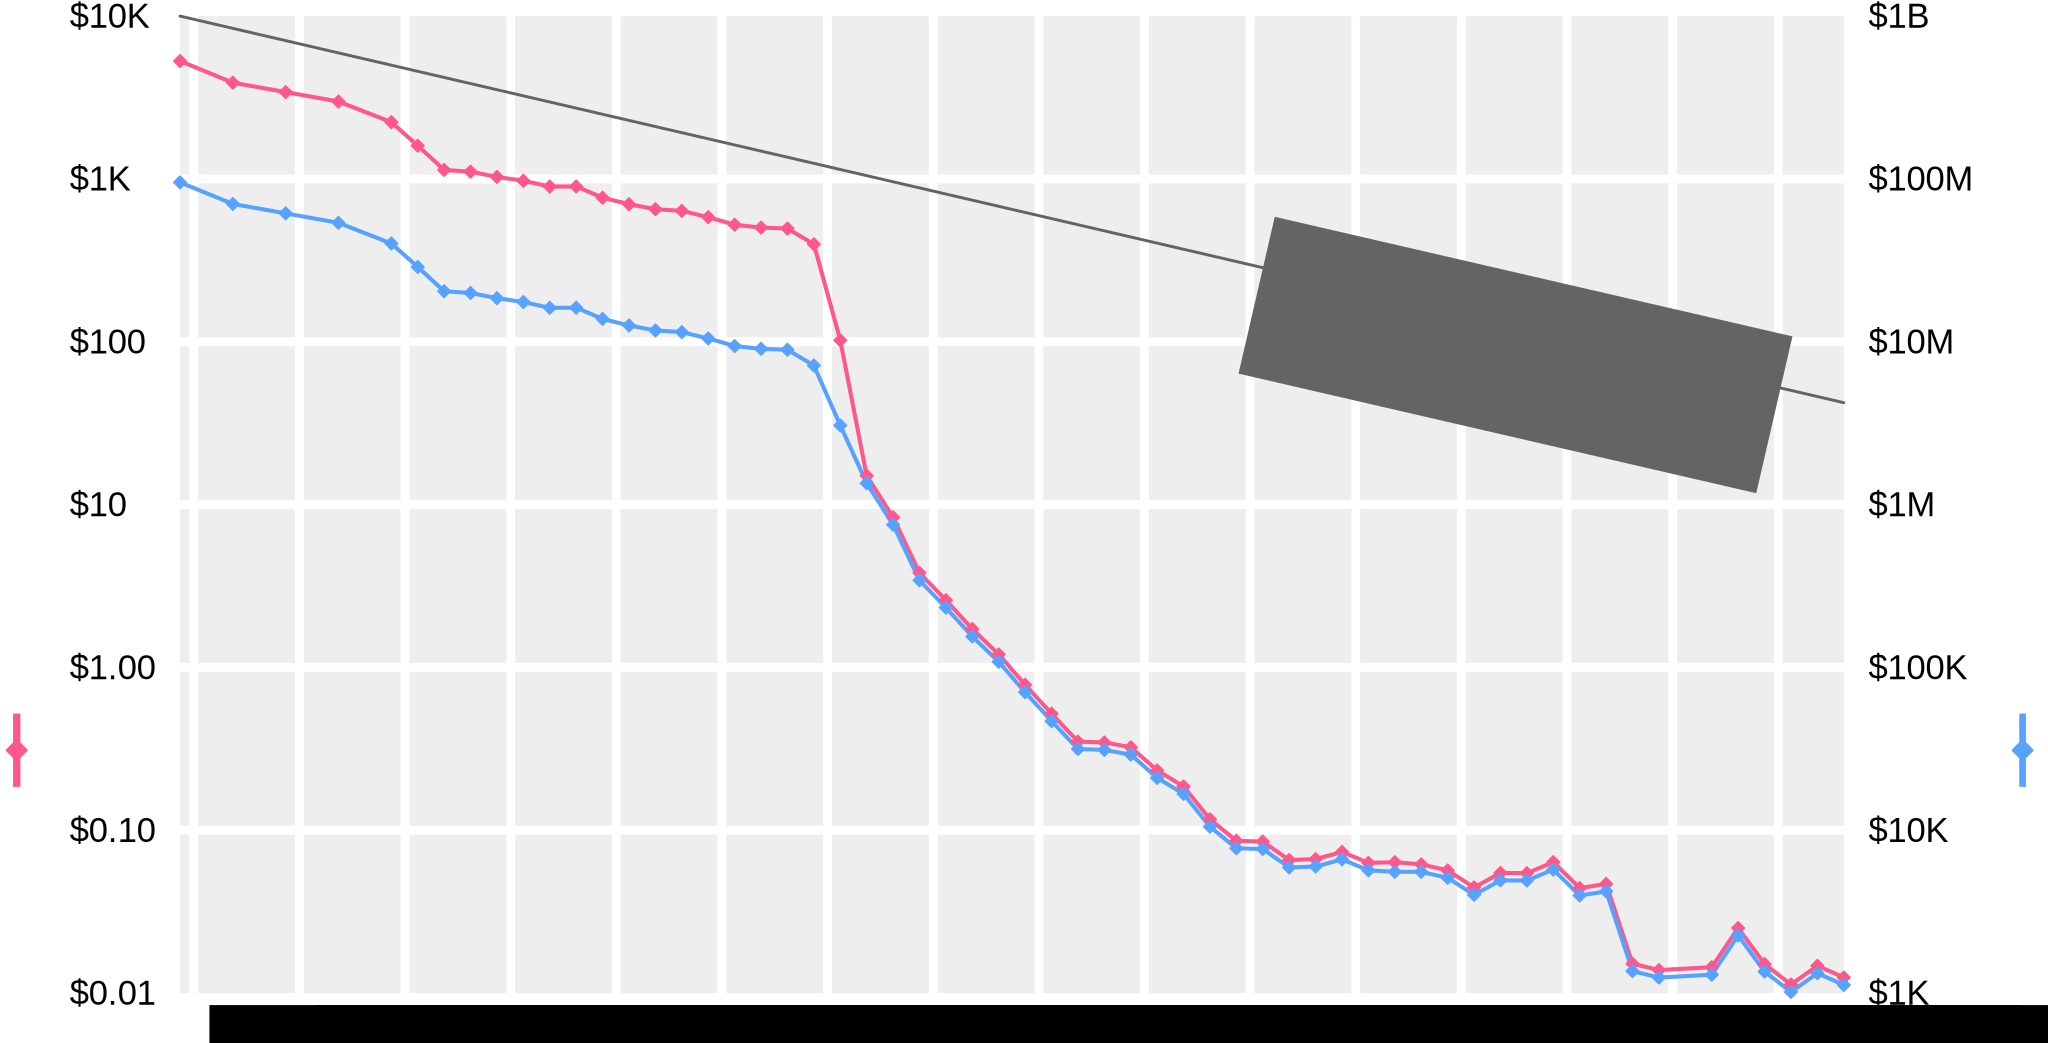
\includegraphics[width=\linewidth]{sequencing_costs.pdf}
    \caption[Sequencing costs per Mbp and per genome]{
        \textbf{Sequencing costs per Mbp and per genome.}
        The cost for DNA sequencing have decreased substantially in the past 15 years.
        The Figure shows the cost per mega-basepair (Mbp) of DNA (red line, left y-axis)
        as well as the cost per human-sized genome of $\approx$\,\num{3}\,Gbp (blue line, right y-axis).
        A basepair represents one character in the DNA.
        Note the logarithmic scaling of the y-axes.
        For comparison, Moore's law \cite{Moore1965} is shown.
        The particularly steep decrease in the beginning of 2008 is caused by
        the adoption of novel (next-generation) sequencing technologies in sequencing centers,
        see \secref{ch:Foundations:sec:SequenceAnalysis:sub:GenomeSequencing}.
        Source: Image based on data from \cite{Wetterstrand2018}.
%         \url{https://www.genome.gov/sequencingcosts/}
%         \url{https://www.genome.gov/sequencingcostsdata/}
    }
    \label{fig:sequencing_costs}
\end{figure}

In particular, these high-throughout technologies allow to directly sequence DNA contained in samples
that have been extracted from environments such as water, soil, or the human gut.
This results in so-called \emph{metagenomic} sequences,
i.e., anonymous DNA sequences from the (microbial) organisms that were present in the environmental sample.
A key question in the analysis of such data is to determine the evolutionary relationships of the sequences.
While these DNA sequences can hypothetically be used to infer phylogenetic trees from scratch,
this approach is limited by several theoretical and practical difficulties:
For instance, typical metagenomic samples contain too many, and too short, sequences
for a feasible and reliable tree inference.

One approach to tackle this issue is the so-called \emph{phylogenetic placement} \cite{Matsen2010,Berger2011},
of metagenomic sequences into a given phylogenetic tree (\secref{ch:Foundations:sec:PhylogeneticPlacement}).
Phylogenetic placement methods classify a set of \emph{query sequences}
into the context of known evolutionary relationships, provided in form of a \emph{reference tree}.
While this information already represents biological knowledge \emph{per se},
it can also be used for further downstream analyses \cite{Matsen2011a}.
The research in this field is however quite young and not many such analysis methods have been developed.

An important task prior to conducting phylogenetic placement of metagenomic sequences is to obtain a suitable
reference phylogenetic tree that captures the biological diversity of the species to be placed.
The assembly of a set of reference sequences from biological databases that can be used to infer such a tree
is typically a manual process, and hence both labor-intensive and potentially error-prone.
This might detain researchers from employing phylogenetic placement in the first place.

Furthermore, while the existing downstream methods for phylogenetic placement
(introduced in \secref{ch:Foundations:sec:PhylogeneticPlacement:sub:ExistingMethods})
allow for in-depth interpretation and visualization of the data,
they were not developed with a particular focus on large-scale studies comprising many thousand environmental samples.
For large datasets, these methods might provide too much detail,
making it hard to interpret results, to spot patterns and clusters in the data,
and to discover correlations with meta-data.

Lastly, the problem of scalability to large datasets does not only affect the methods themselves.
Because of the ever growing amount of sequence data,
scalability is becoming an issue for the software pipelines as well.
State-of-the-art phylogenetic placement implementations can place billions of sequences within a few hours \cite{Barbera2018}.
Methods for processing and analyzing the data, in particular phylogenetic placement data,
hence require efficient and scalable software implementations.

% ######################################################################################################################
%         Objective and Contribution
% ######################################################################################################################

\section{Objective and Contribution}
\label{ch:Introduction:sec:ObjectiveContribution}

in this thesis...

\chpref{ch:AutomaticTrees}

\chpref{ch:Visualization}

\chpref{ch:Clustering}

we developed methods for working with such data, and helped to conduct several empirical studies using established as well as our novel methods.

method papers (main contrib for this work, see next section)
phat \cite{Czech2018}
vis clust \cite{Czech2018a}



tree viz review \cite{Czech2017}



method and software dev:

salt \cite{Flouri2017}

unieuk \cite{Berney2017}

tree clustering workshop?

epa ng \cite{Barbera2018}

quartet score \cite{Zhou2017}

swarm code contrib \cite{Mahe2014,Mahe2015}

scrapp




data analysis:

1kite \cite{Misof2014}
\url{http://1kite.org}

neotrop \cite{Mahe2017}

microsopirida \cite{Bass2018a}

long reads (in prep)

dinos (in prep)




mention genesis and gappa, their implementation chapter in the appendix,
their paper?!
github links
\url{https://github.com/lczech/genesis}
\url{https://github.com/lczech/gappa}

genesis: implements some established methods, just way faster

mention  \url{http://github.com/lczech/placement-methods-paper} for the result files of two of the papers

full list of publications is available in \secref{ch:Publications}

% ######################################################################################################################
%         Structure and Overview
% ######################################################################################################################

\section{Structure and Overview}
\label{ch:Introduction:sec:StructureOverview}


\todo{check that the url and access date of all online sources are present in bibliography!}

% \todo{I used a few public domain images from wikipedia as sources, and modified them as needed. make sure that this is okay.}

\todo{search for all abbreviations used and add them to the acro list. also, check Pierre's MA, and Alexey's and Andre's Diss for needed acronyms!}
\todo{list of acronyms!} see andre, add MB/GB, PCA,
BV, TO, HMP, etc

\todo{unify table and figure caption capitalization}

\todo{more workflow flow charts?}

% ######################################################################################################################
%         Foundations
% ######################################################################################################################

\chapter{Foundations}
\label{ch:Foundations}

\paperbox{
    This chapter is partially based on the peer-reviewed publications:
}{\paperart \paperpppp}{
    \todo{
        \textbf{Contributions:} Lucas Czech... Pierre Barbera... Alexandros Stamatakis... and...
    }
}

\todo{In this chapter, we introduce\ldots}

% ######################################################################################################################
%         Evolution and Genetics
% ######################################################################################################################

\section{Evolution and Genetics}
\label{ch:Foundations:sec:EvolutionGenetics}

% Evolution is change in the heritable characteristics of biological populations over successive generations.
% \url{https://en.wikipedia.org/wiki/Evolution}
% the process by which new species or populations of living things develop from preexisting forms through successive generations
% \url{https://www.merriam-webster.com/dictionary/evolution}
% Evolution is a process of continuous branching and diversification from common trunks. This pattern of irreversible separation gives life's history its basic directionality. —Stephen Jay Gould
% \url{https://www.merriam-webster.com/dictionary/evolution}

% Evolution is the continuous process of diversification of biological populations through successive generations \cite{Hall2008}.

Life on Earth is at least 3.77 billion years old \cite{Dodd2017},
and is continuously evolving due to \emph{natural selection} \cite{Darwin1859}.
% Woah, I like that very first sentences. A very old and a very new publication, binding all of reasearch together...
Driven by \emph{variation}, biological populations diversify through successive generations,
leading to the origination of new species.
This continuous process is called \emph{evolution} \cite{Hall2008}.
Heritable characteristics are passed down from parent to offspring,
with occasional random mutations leading to variation.
Thus, some organisms are better adapted to their environment than others,
and have more reproductive success.
There is hence a natural selection for advantageous mutations,
which can then spread through generations.

% this process was not understood for a long time. static species?
% four driving forces of pop gen?

The characteristics and traits of an organism are carried by, and inherited via, \emph{deoxyribonucleic acid} (DNA).
DNA is the molecule that encodes the genetic information needed for the functioning of all living organisms.
It is structured in form of a double helix \cite{Watson1953},
and built from two strands of molecules called \emph{nucleotides}.
The nucleotides build the backbone of the double helix,
and connect the two strands via opposing pairs of \emph{nucleobases}, see \figref{fig:dna_nucleobases:sub:dna_helix}.
The redundant structure of pairs of nucleobases gives stability to the DNA molecule,
and also serves as a mechanism of error correction when reading the genetic information during cellular processes.
% both of which is important for the role of DNA for information storage.
In DNA, there are four distinct nucleobases:
adenine (\nucleobase{A}), cytosine (\nucleobase{C}), guanine (\nucleobase{G}), and thymine (\nucleobase{T}),
where \nucleobase{A} pairs with \nucleobase{T}, and \nucleobase{C} pairs with \nucleobase{G}, respectively,
as shown in \figref{fig:dna_nucleobases:sub:nucleobases}.

\begin{figure}[hpbt]
    \centering
    \includegraphics[width=.7\linewidth]{dna_nucleobases.pdf}
    \begin{subfigure}{0pt}
        \phantomcaption
        \label{fig:dna_nucleobases:sub:dna_helix}
    \end{subfigure}
    \begin{subfigure}{0pt}
        \phantomcaption
        \label{fig:dna_nucleobases:sub:nucleobases}
    \end{subfigure}
%     \begin{subfigure}{0pt}
%         \phantomcaption
%         \label{fig:dna_nucleobases:sub:transition_transversion}
%     \end{subfigure}
    \caption[DNA double helix and nucleobases]{
        \textbf{DNA double helix and nucleobases.}
        \subref{fig:dna_nucleobases:sub:dna_helix}
        The double helix structure of DNA, with the backbone in gray,
        connected by pairs of nucleobases.
        \subref{fig:dna_nucleobases:sub:nucleobases}
        The atomic structure of the four nucleobases, and their connection to each other.
%         Note that the diameter of the helix is about \SI{2}{\nano\meter}.
        Source and license: see \cite{Czech2018DNA},
        image derived from \cite{MesserWoland2006,Sponk2010,Yikrazuul2008a,Yikrazuul2008b}.
%         \\
%         Source: Image derived from \cite{Yikrazuul2008a,Yikrazuul2008b}.
%         Source: Image derived from \cite{Sponk2010}.
%         \subref{fig:dna_nucleobases:sub:transition_transversion}
%         Each nucleobase can mutate into any other in the course of evolution.
%         The two different types of mutation (transitions vs. transversions) are not equally likely,
%         due to physical properties of the nucleobases.
    }
    \label{fig:dna_nucleobases}
\end{figure}

% Transitions vs Transversions - not needed
% Over the course of evolutionary times, mutations in the DNA occur, mainly due to errors in the replication process.
% These mutations manifest in form of changed nucleobases.
% There are two types of mutations, \emph{transition} \emph{transversions}, which are not equally likely.
% \cite{Futuyma2013}
% \figref{fig:dna_nucleobases:sub:transition_transversion}

The sequence of nucleobases along the strands of DNA is what encodes the genetic instructions
used by all known living organisms.
Parts of the DNA encode for proteins,
which perform a plethora of different functions within organisms.
Proteins consist of long chains of amino acid residues, and
are assembled in a process called protein (bio)synthesis.
This is described by the central dogma of molecular biology \cite{Crick1958,Crick1970}:
First, DNA is \emph{transcribed} into the intermediary ribonucleic acid (RNA),
which is then \emph{translated} into the actual protein.

In each step of this process, the molecular alphabet used to encode information differs.
While DNA uses the four nucleobases as described above,
in RNA, the nucleobase uracil (\nucleobase{U}) is used instead of thymine (\nucleobase{T}).
Proteins on the other hand are (mostly) build from a set of \num{20} standard amino acids.
The set of rules used by the molecular machinery for translating nucleobases into amino acids
is called the \emph{genetic code}:
In a DNA sequence, three consecutive nucleobases are needed to encode one amino acid \cite{Shu2017}.

The entirety of the genetic material of an organism, that is, its complete DNA sequence, is called its \emph{genome}.
A \emph{gene} is a sequence which codes for a molecule that has a particular function, such as a protein \cite{Gericke2007}.
DNA and genes are the basic units of heredity.
They are what is varying across generations,
and what is selected for in the process of natural selection \cite{Dawkins1989}.
The study of genes, variation and heredity is called \emph{genetics} \cite{Griffiths2000}.

% ######################################################################################################################
%         Sequence Analysis
% ######################################################################################################################

\section{Sequence Analysis}
\label{ch:Foundations:sec:SequenceAnalysis}

All life on this planet is related to each other and descends from a common ancestor.
Still, it is remarkable that the basic molecular principles and mechanisms of life---%
DNA, amino acids, and the genetic code---are virtually identical for all living organisms.
This implies that by understanding and comparing the genetic information
encoded in the genetic sequences of different organisms,
one can understand the diversification patterns of evolution.

% ======================================================================================================================
%     Genome Sequencing
% ======================================================================================================================

\subsection{Genome Sequencing}
\label{ch:Foundations:sec:SequenceAnalysis:sub:GenomeSequencing}

Prior to analyzing the DNA of an organism, the physical order of nucleobases in the DNA molecule has to be determined.
That is, the DNA has to be ``read'' and stored in a human-accessible text format, typically a computer file.
This technical process is called DNA \emph{sequencing}.
% which can be understood as putting biomass into a blender and converting it into text files ;-)

For many decades, the main technique for this purpose was Sanger sequencing \cite{Sanger1975,Sanger1977}.
It is labor- and time-intensive, but through improvement and automation, costs were constantly reduced.
Eventually, this allowed for large-scale efforts, such as the Human Genome Project \cite{Venter2001},
which sequenced the whole human genome of more than three billion nucleobases.
Sanger sequencing allows to determine long parts of the sequence at once (> \num{500} nucleobases),
which then have to be assembled to build the final sequence.

In the last decades, a variety of novel high-throughput DNA sequencing technologiesß
have been developed \cite{Pettersson2009,Reuter2015,Goodwin2016}.
In particular, \emph{Next Generation Sequencing} (NGS) \cite{Logares2012,Mardis2013}
has revolutionized biology by transforming it into a data-driven and compute-intense discipline \citep{Escobar-Zepeda2015}.
The costs of these technologies are decreasing faster than Moore's law \cite{Wetterstrand2018}.
This leads to a ``tsunami'' of sequence data,
which poses a challenge for computational methods working with these data.
Compared to Sanger sequencing, NGS technologies are generally cheaper and faster \cite{Voelkerding2009,Metzker2010},
but come at the price of introducing more errors in the sequence output,
or only being able to determine shorter parts of the sequence at once
-- both of which constitute a challenge for the subsequent assembly of the final sequence.

The result of DNA sequencing is a textual representation of the order of nucleobases.
Although this representation ignores the physical and chemical properties of the respective molecules,
it is helpful in many applications, and allows to leverage existing algorithms.
Each contiguous sequence coming from the sequencing machine is called a \emph{read}.
Because of the pairing of nucleobases,
both DNA strands can be sequenced, which provides a means of error correction.
Such data are typically stored in the \fileformat{fastq} file format \citep{Cock2009}.
These so-called paired-end reads are then merged to form a final sequence representation of one strand
% cite \toolname{PEAR} \cite{Zhang2014} ?
-- that is, a sequence of the characters \nucleobase{A}, \nucleobase{C}, \nucleobase{G}, and \nucleobase{T}.
These data are stored in formats such as the \fileformat{fasta} file format \citep{Pearson1988}.
Due to the pairing of nucleobases,
the length of a DNA sequence is measured in \emph{base pairs} (abbreviated \si{\basepair}):
\SI{1}{\basepair} represents one character in the file.
These files are then the input for computational methods for working with DNA sequences.

% Not needed right now:
% Because of the universal genetic code of translating DNA to amino acids,
% it is also possible to store the amino acid sequence instead of the nucleobase sequence.

% ======================================================================================================================
%     Metagenomics
% ======================================================================================================================

\subsection{Metagenomics}
\label{ch:Foundations:sec:SequenceAnalysis:sub:Metagenomics}

Sanger sequencing requires careful preparation of the genetic material,
and is thus best used for sequencing single organisms.
There are however many (microbial) organisms that cannot be cultured in a Petri dish,
and are hence hard to sequence with this technique.
Apart from being cheaper, Next Generation Sequencing machines however ``digest'' all genetic material presented to them.
They thus allow for studying microbial samples
directly extracted from their environment \citep{Morgan2010,Edwards2013,Sunagawa2013a}.
This enables to study environments such as
water \cite{Karsenti2011,Giner2016,Gran-Stadniczenko2017},
soil \cite{Dupont2016,Mahe2017},
the human body \cite{Huttenhower2012,Methe2012,Matsen2015,Wang2015},
and many others.
Each sample from such an environment then represents a geographical location, a body site, a point in time, etc.
% These studies yield a large set of short anonymous DNA reads for each sample.
% The DNA reads obtained from sequencing a sample represent all organisms present in the sample;
The DNA of all organisms being present in a sample is sequenced,
resulting in a large number of reads per sample.
These reads are anonymous, as it is unclear to which organism they originally belonged.
The study of these data, that is, genetic material from environmental samples, is called \emph{metagenomics} \cite{Oulas2015}.

% \paragraph{Key Tasks}
% \label{ch:Foundations:sec:SequenceAnalysis:sub:Metagenomics:par:KeyTasks}

% A first step is often to generate a genetic profile of the environment,
% that is, to estimate the diversity of the organisms in the sample.
A first step in metagenomic studies is often to characterize the reads obtained from an environment
in terms of \emph{reference sequences} of known species.
Reads that are similar to (parts of) reference sequences can be assigned to them,
while reads with low similarity to known sequences might indicate novel, undescribed species \cite{Temperton2012}.
Key tasks in metagenomic studies are the identification and classification of the anonymous reads (``Who is there?''),
and their functional annotation (``What are they doing?'') \cite{Desai2012}.
Both are introduced in the following.

% The following paragraph is not totally needed, as we are not doing functional analysis.
% However, it introduces many other terms alongside, which is useful later on.
Functional annotation \cite{Stein2001} is the prediction of gene functions of the reads,
and the inference of metabolic capacity of microbial communities \cite{Brown2017}.
As the proteins that are needed in the pathways of such functions can be encoded by genes across the genome,
whole-genome sequencing is necessary to capture all genes of interest.
For example, in shotgun sequencing \cite{Staden1979,Anderson1981},
the DNA is fragmented into small pieces within the size range that the used sequencing technology can handle,
typically a few hundred \si{\basepair} long.
This allows to sequence all genetic material contained in a sample.
Thus, the resulting reads originate from different parts of the genomes of their organisms,
which can then be functionally annotated \cite{Glass2010}.
This however necessitates to use whole-genome reference sequences
in order to be able to assign reads to known species and functions.
Typical databases of reference sequences however
lack many of the protein sequences from the microbial species present in a sample,
mostly because of organisms that cannot be cultured \cite{Brown2017}.

For the task of identification and classification of reads however, whole genome references are not needed.
Instead, specific \emph{marker genes} can be used,
which are regions of genes that are particularly suited for delineating between different species \cite{Ren2016}.
% highly conserved, that is, slowly changing over evolutionary times.
% but certain parts are radpidly evolung (hyper variable) withing the region, which is good for delineation.
% typically, this is general basic cell functionen stuff, which is needed by many forms of live.
% eg cell division, ssu... mitochondrial dna, etc
The method of using marker genes to identify species is called \emph{DNA barcoding} \cite{Hebert2003,Savolainen2005,Deiner2017b}.
The choice of genes to use as marker is important, and depends on the types of organisms to be studied.
The used marker genes should ideally be present in all of the organisms of interest,
short enough to be sequenced with current technology,
and have enough variation between species to distinguish between them,
but have low variation within species \cite{Kress2008}.

% \paragraph{Typical Processing}
% \label{ch:Foundations:sec:SequenceAnalysis:sub:Metagenomics:par:TypicalProcessing}

In many metagenomic studies of \taxonname{bacteria} and \taxonname{eukaryota},
the 16S \cite{Weisburg1991} and 18S \cite{Meyer2010} rRNA regions are used as marker genes,
respectively \cite{Woese1977,Woese1990}.
These regions belong to the small subunit (SSU) of the ribosomal ribonucleic acid (rRNA),
which is an essential component of the ribosome.
The ribosome is a molecular machinery that is responsible for protein synthesis (translation) in all living organisms.
% and are thus present in virtually all \taxonname{bacteria} and \taxonname{eukaryota}.
Often, prior to sequencing, these regions are amplified by many orders of magnitude,
using polymerase chain reaction (PCR) to create copies of these regions \cite{Bartlett2003}.
The resulting reads are then de-replicated again, which results in sequences called \emph{amplicons}.
While the PCR amplification process is known to introduce bias \cite{Logares2014,Brown2017},
this inexpensive method is commonly used in practice, particularly for the 16S and 18S rDNA regions.
A recent alternative to using PCR for obtaining reads from these regions are \textsubscript{mi}tags \citep{Logares2014}.
In this approach, shotgun sequencing is used to get reads from the whole genomes of the organisms in a sample.
These reads are then filtered to only contain reads from the 16S region (for \taxonname{bacteria}),
which capture the diversity of the sample without bias.

Because of the ubiquity of the 16S and 18S rDNA regions in organisms and, consequently, in sequencing studies,
many databases provide reference sequences for these marker regions.
The reads or amplicons obtained from an environmental sample can then be employed
to estimate the microbial diversity of the organisms in the sample by comparison against known species.

% ======================================================================================================================
%     Sequence Alignments
% ======================================================================================================================

\subsection{Sequence Alignment}
\label{ch:Foundations:sec:SequenceAnalysis:sub:SequenceAlignment}

Organisms that evolved from a (not too distant) common ancestor share genetic information.
Regions of their DNA that have a shared ancestry are called \emph{homologous} regions \cite{Koonin2005}.
This homology is typically inferred from sequence similarity. %, that is, by comparison of the sequences.
However, due to mutations, differences in the sequences can occur.
There are three main types of sequence mutations that can occur in evolution:
a \emph{substitution} is the exchange of a nucleobase for another;
a \emph{insertion} adds one or more extra nucleotides into the sequence;
a \emph{deletion} removes one or more nucleotides from the sequence.
The latter two types of mutations change the length of the sequence;
a mutation that is either one of them is called an \emph{indel}.

Because of indels, sequences have to be aligned to each other in order to compare their homologous regions.
That is, gap characters (\nucleobase{-}) have to be added to the sequences
such that homologous characters in the sequence get aligned.
This results in an $n \times m$ matrix,
where $n$ is the number of sequences (rows),
and $m$ is the number of homologous characters (columns), called \emph{sites}.
This matrix is called a \emph{multiple sequence alignment} (MSA), or simply an \emph{alignment}.
\figref{fig:msa} shows an example of the alignment process and the resulting MSA.

\begin{figure}[hpbt]
    \centering
%     \vspace*{0.5em}
    \includegraphics[width=.9\linewidth]{msa.pdf}
    \caption[Multiple Sequence Alignment]{
        \textbf{Multiple Sequence Alignment.}
        The left hand side shows a set of six sequences.
        Using an alignment algorithm, gaps are inserted into these sequences at presumed indel positions.
        The right hand side shows the result of this process,
        where homologous characters at the sites of the multiple sequence alignment (MSA) are aligned to each other.
        Below the MSA, the majority rule consensus sequence is shown,
        see \secref{ch:Foundations:sec:SequenceAnalysis:sub:ConsensusSequences}.
    }
    \label{fig:msa}
\end{figure}

Sequence alignment can be understood as an optimization problem under a given optimality criterion.
On the one hand, \emph{global alignments} attempt to align every character in every sequence,
which is most useful for similar sequences of roughly equal size.
For example, the Needleman-Wunsch algorithm \cite{Needleman1970} is a general global alignment technique
based on dynamic programming.
On the other hand, \emph{local alignments} are better suited for dissimilar sequences
which might contain similar regions within a larger sequence context.
The Smith-Waterman algorithm \cite{Smith1981} is a general local alignment technique
using the same dynamic programming scheme,
which additionally allows to start and end at any place in the sequence.
As both algorithms have their particular use cases \cite{Polyanovsky2011},
hybrid methods have also been developed \cite{Brudno2003}.
Furthermore, heuristic approaches such as \toolname{BLAST} \cite{Altschul1990} and
\toolname{USEARCH} \cite{Edgar2010} can calculate millions of near-optimal alignments in reasonable time.

These algorithms are efficient for the pairwise alignment of two sequences.
Calculating an MSA however has been shown to be NP-hard \cite{Wang1994,Just2001}.
Thus, for most empirical data sets, other approaches and heuristics are needed \cite{Thompson2011}.
Tools such as \toolname{CLUSTAL} \cite{Higgins1988}, \toolname{MUSCLE} \cite{Edgar2004}, and \toolname{MAFFT} \cite{Katoh2002}
can calculate near-optimal multiple sequence alignments for many thousands of sequences.

A special use case for aligning sequences arises in metagenomic studies,
where environmental sequences are often compared to a set of known reference sequences.
In these studies, one often first calculates an MSA of the reference sequences,
and then successively aligns the environmental sequences against this MSA.
This is because calculating an MSA for millions or billions of sequences from scratch is too expensive even for modern tools.
Hence, specialized algorithms for this use case have been developed,
such as \toolname{PaPaRa} \citep{Berger2011a,Berger2012} and
\toolname{hmmalign}, which is a subprogram of the \toolname{HMMER} suite \citep{Eddy1998,Eddy2009}.

% ======================================================================================================================
%     Consensus Sequences
% ======================================================================================================================

\subsection{Consensus Sequences}
\label{ch:Foundations:sec:SequenceAnalysis:sub:ConsensusSequences}

When working with a number of related but not identical sequences,
it is often convenient to ``summarize'' homologous characters in form of a \emph{consensus sequence}.
Such a sequence is typically calculated based on the relative frequencies of the characters per alignment site.
It then represents typical features and motifs of the input set of sequences.

The most straight forward method is to construct \emph{majority rule consensus} sequences \citep{May1952,Day1992a},
where each site is represented by the most frequent character at that site.
\figref{fig:msa} shows an example below the MSA on the right hand side.
In order to also include information from the less frequent characters at a site in the consensus sequence,
\emph{ambiguity characters} can be used \cite{IUPAC1970}.
They allow to denote multiple alternative nucleobases as a single character.
For example, if the nucleobases \nucleobase{A} and \nucleobase{G} are similarly frequent at a site,
this site is represented by the ambiguity character \nucleobase{R}.
See \tabref{tab:AmbiguityCharacters} for the full list of character representations.

Using ambiguity characters allows for more involved consensus methods.
For example, \emph{threshold consensus} sequences \citep{Day1992a,Day1992} include the most frequent characters
that are needed to achieve some given frequency threshold per site,
and represent these characters by their ambiguity character.
Furthermore, many methods based on fixed thresholds have been proposed,
such as Cavener's method \citep{Cavener1987,Cavener1991a};
see \cite{Day1992a} for a critical comparison.

It is theoretically also possible to directly use the relative frequencies of characters per site
in the mathematical frameworks of many downstream analysis methods.
This would allow to leverage all of the information contained in the input set of sequences.
However, to our knowledge, there is no convention or file format to store such information,
and consequently, no way of forwarding this information to the respective tools.

% ######################################################################################################################
%         Tree of Life
% ######################################################################################################################

\section{The Tree of Life}
\label{ch:Foundations:sec:TreeOfLife}

The shared evolutionary history of life gives rise to a branching pattern,
where new \emph{lineages} split from a common ancestor.
This branching pattern forms a tree-like structure,
which classifies organisms in a hierarchy based on common descent.

While this \emph{tree of life} is an expedient and, hence, pervasive model \cite{Mindell2013},
it ignores certain biological and evolutionary events.
A strict hierarchy does not allow for reticulate events,
such as hybridization \cite{Maddison1997a}, genetic recombination \cite{Hein1993},
or horizontal gene transfer \cite{Ochman2000,DunningHotopp2011,Robinson2013}.
Although approaches such as networks have been proposed to model these events \cite{Huson2011a},
the simplicity of a hierarchy or tree structure still has proven
to be useful in classifying and naming organisms, and understanding their evolutionary relationships.

% not considering lat gene tranfs, there is only one ``true'' tree of life.

% For the \taxonname{eukaryota}, the tree model is still considered valid.
% However, \taxonname{bacteria} have the ability of horizontal gene transfer,
% where genetic information is transferred between unrelated organisms.

% biology is messy: https://www.ncbi.nlm.nih.gov/pubmed/20852602

% ======================================================================================================================
%     Taxonomy and Nomenclature
% ======================================================================================================================

\subsection{Taxonomy and Nomenclature}
\label{ch:Foundations:sec:TreeOfLife:sub:TaxonomyNomenclature}

Early attempts at classifying organisms date back to the Greek philosopher Aristotle,
who used observable attributes to divide living things into groups \cite{Leroi2014}.
This approach as well as the efforts of later centuries were non-uniform and inconsistent.
The basis for the modern system of classification was established
by Swedish botanist Carl Linnaeus in the mid-18th century \cite{Donk1957}.
He proposed a \emph{nomenclature}, that is, a naming system for organisms,
as well as a \emph{taxonomy}, that is, a rank-based classification of organisms \cite{Linnaeus1735,Linnaeus1753}.

A taxonomic group of organisms is called a \emph{taxon} (plural: \emph{taxa}).
Each taxon is associated with a \emph{taxonomic rank}, which can subsume other ranks,
thus forming a hierarchy of higher and lower ranks.
A taxonomic rank represents the relative level of a group of organisms in the taxonomy.
The principal ranks in modern use are \taxonname{domain}, \taxonname{kingdom}, \taxonname{phylum}, \taxonname{class},
\taxonname{order}, \taxonname{family}, \taxonname{genus}, and \taxonname{species},
see \figref{fig:taxonomic_ranks}.
If needed, further ranks can be included in between (such as \emph{sub-genus}),
or more refined lower levels be added (such as \emph{strain}, which is a further distinction within a species).

\begin{figure}[hpbt]
    \centering
%     \vspace*{0.5em}
    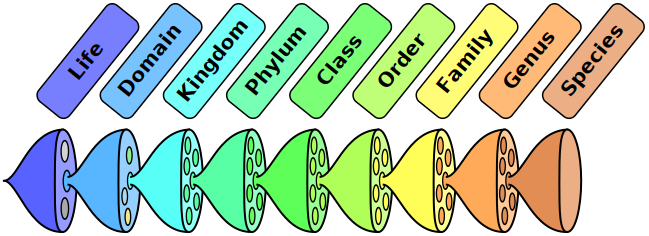
\includegraphics[width=.85\linewidth]{taxonomic_ranks.pdf}
    \caption[Biological classification into taxonomic ranks]{
        \textbf{Biological classification into taxonomic ranks.}
        The figure depicts a typical set of nested taxonomic ranks \cite{Woese1990},
        which form a hierarchy with increasingly deeper levels towards the right.
%         The taxonomic ranks shown here follow the three-domain system \cite{Woese1990}.
%         which classifies cellular life into the domains \taxonname{archaea}, \taxonname{eukaryota}, and \taxonname{bacteria}.
%         The deeper levels towards the right form a hierarchy of nested taxonomic ranks.
        Source: Image derived from \cite{Halasz2007}.
    }
    \label{fig:taxonomic_ranks}
\end{figure}

In order to scientifically name the groups of organisms (taxa) in a taxonomy,
the \emph{binomial nomenclature} as introduced by Linnaeus is still prevalent to this day.
It uses two terms, often of Latin origin,
which respectively specify the taxonomic ranks \emph{genus} and \emph{species} that an organism belongs to,
for example \taxonname{Homo sapiens}.

While early classifications used \emph{phenotypes}, that is, observable characteristics or traits of organisms,
modern approaches to taxonomy take genetic information into account \cite{Mayr2002}.
For example, the three-domain system \cite{Woese1977,Woese1990} resolves the oldest evolutionary relationships,
that is, the highest taxonomic levels, based on 16S rRNA data.
Although this classification has been challenged \cite{Gupta1998,Mayr1998,Cavalier-Smith2002}, it is widely used.
It divides cellular life forms into the three domains \taxonname{bacteria}, \taxonname{archaea}, and \taxonname{eukaryota};
the latter is further separated into kingdoms,
which include the kingdoms \taxonname{fungi}, \taxonname{plants}, and \taxonname{animals}.

% Archaea, Domain (and Kingdom)
% Eukarya, Domain
% Protista, Kingdom
% Fungi, Kingdom
% Animalia, Kingdom
% Plantae, Kingdom
% Bacteria, Domain (and Kingdom)

% ======================================================================================================================
%     Phylogenetic Trees
% ======================================================================================================================

\subsection{Phylogenetic Trees}
\label{ch:Foundations:sec:TreeOfLife:sub:PhylogeneticTrees}

The classification of organisms into a taxonomy is based on (subjective) dissimilarity and thus arbitrary:
The number of organisms that are grouped into a taxon at a given rank can vary,
and the separation into discrete ranks does not reflect the gradual nature of evolution \cite{Gingerich1987}.
A more involved approach that can resolve these issues is \emph{phylogenetics},
which is the study of the evolutionary history and relationships of biological entities (individuals, species, populations).

The evolutionary relationships of such entities are called their \emph{phylogeny}.
As the true phylogeny of a set of taxa is unknowable,
it has to be inferred from data that is available.
A phylogenetic analysis uses inference methods that evaluate observed heritable traits
in order to resolve the phylogeny under a given model of evolution of these traits.
While phenotypes can be used, modern phylogenetic inference is mostly based on DNA data.
The result of a phylogenetic analysis is a \emph{phylogenetic tree},
also called an \emph{evolutionary tree}, or---synonymously---a \emph{phylogeny}.
\figref{fig:tree_of_life} shows two examples of phylogenetic trees.

\begin{figure}[hpbt]
    \centering
    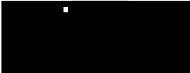
\includegraphics[width=\linewidth]{tree_of_life.pdf}
    \begin{subfigure}{0pt}
        \phantomcaption
        \label{fig:tree_of_life:sub:darwin}
    \end{subfigure}
    \begin{subfigure}{0pt}
        \phantomcaption
        \label{fig:tree_of_life:sub:woese}
    \end{subfigure}
    \caption[Exemplary phylogenetic trees]{
        \textbf{Exemplary phylogenetic trees.}
        \subref{fig:tree_of_life:sub:darwin}
        In 1837, Charles Darwin sketched his first evolutionary tree below the words ``I think''
        in his notebook on ``Transmutation of Species''.
        Source: Image derived from \cite{DarwinTreeOfLife1837}.
%         \\
        \subref{fig:tree_of_life:sub:woese}
        A modern phylogenetic tree showing the three-domain system \cite{Woese1977,Woese1990},
        which emphasizes the separation of \taxonname{bacteria}, \taxonname{archaea}, and \taxonname{eukaryota}
        based on 16S rRNA genes.
        The black branch at the bottom represents the speculative last universal common ancestor of all living organisms.
        Source: Image derived from \cite{WoeseTreeOfLife2006}.
    }
    \label{fig:tree_of_life}
\end{figure}

\paragraph{Properties of Trees}
\label{ch:Foundations:sec:TreeOfLife:sub:PhylogeneticTrees:par:TreeProperties}

The leaf nodes, or \emph{tips}, of the tree represent living (\emph{extant}) biological entities
such as species, strains, individual organisms, or even cells of a multicellular organism.
Thus, the tips are often referred to as the \emph{taxa} of the tree,
which is meant as a generic term that includes all the above entities.
The tips are often named according to the entities they represent (e.\,g., species names);
such a tree is called a \emph{labeled} tree.
The inner nodes on the other hand are usually anonymous and
represent speciation events, where two novel lineages arose from a putative common ancestor.
The branching pattern of a phylogenetic tree thus reveals the evolutionary history of its taxa.

The edges of the tree, also called its \emph{branches}, can have associated \emph{branch lengths},
which represent the evolutionary time between the two adjacent nodes,
for example, measured as the average change in nucleobases between their respective sequences.
The unique path between any two nodes thus can be interpreted
as a measure of evolutionary relatedness of the taxa represented by the nodes.

A phylogenetic tree is \emph{rooted}
if it is a directed tree that has a unique \emph{root node},
which corresponds to the putative common ancestor of the other nodes in the tree.
See \figref{fig:tree_of_life:sub:woese} for an example.
As evolution is a processes that happens over time,
from a biological point of view, every tree has a root.
However, most models of DNA evolution are time-reversible,
meaning that the direction of change in the sequences cannot be inferred from the data under such models,
see \secref{ch:Foundations:sec:MLTreeInference:sub:ModelsOfSeqEvol} for details.
Thus, tree inference methods can also yield \emph{unrooted} trees without direction and without a root node.
In these methods, for computational reasons, often a \emph{virtual root} is used,
which is a hypothetical additional node placed on a branch of the tree.
For tasks such as traversing a tree, but also in order to store a tree in a file,
unrooted trees usually have a distinguished, but arbitrary, ``starting'' node called a \emph{top-level trifurcation}.
An unrooted tree can be rooted a posteriori, for example by using an \emph{outgroup} of taxa
that are closely related to the group of taxa of interest (the \emph{ingroup}), but not part of it.
Then, a root node can be placed on the branch that separates the outgroup from the ingroup.

An inner node that has exactly three neighboring nodes is called a \emph{bifurcation} or a \emph{bifurcating} node.
In rooted trees, these neighbors are the the parent and the two children of a node, hence the name.
An inner node with more neighbors is called a \emph{multifurcation} or a \emph{multifurcating} node.
This naming also applies to the whole tree:
A tree, where each inner node (with the exception of the root node in a rooted tree) is bifurcating,
is also called a bifurcating tree.
Otherwise (if there is at least one multifurcating node), it is a multifurcating tree.
Note that in evolution, an actual multifurcation event is highly unlikely,
as it corresponds to the simultaneous formation of more than two new lineages from a single ancestral lineage.
Multifurcating trees are for example used when relationships cannot be properly resolved from the existing data,
or to summarize a set of otherwise contradicting trees.

Each edge of the tree induces a \emph{bipartition} or \emph{split} of the taxa of the tree into two groups,
one on each side of the edge.
A set of taxa is \emph{monophyletic},
if there is a bipartition of the tree that splits these taxa from all other taxa of the tree.
In a rooted tree, the node at the end of that edge is then the putative common ancestor of these taxa.
Furthermore, a monophyletic set of taxa is called a \emph{clade} of the tree;
in other words, a clade is a subtree that is separated from the rest of the tree by one edge.
For example, the taxa {\sffamily A}, {\sffamily B}, and {\sffamily C} in \figref{fig:tree_vis_options} are monophyletic---%
that is, they form a clade of the tree.
Lastly, a non-monophyletic set of taxa is \emph{paraphyletic}.

\paragraph{Practical Aspects of Trees}
\label{ch:Foundations:sec:TreeOfLife:sub:PhylogeneticTrees:par:PracticalAspects}

While the topology of the tree is what models the evolutionary relationships,
there are several ways of visualizing or drawing that information.
\figref{fig:tree_vis_options} shows some examples, which all visualize the same topology (except for the rooting).
The figure also summarizes some of the terms and concepts introduced above.
Different drawing styles each have their advantages.
For example, in a rectangular tree (\figref{fig:tree_vis_options:sub:rectangular}),
branch lengths are easier to read and compare,
while a circular tree (\figref{fig:tree_vis_options:sub:circular}) can fit more taxa in the same drawing area.

\begin{figure}[hpbt]
    \centering
    \includegraphics[width=\linewidth]{tree_vis_options.pdf}
    \begin{subfigure}{0pt}
        \phantomcaption
        \label{fig:tree_vis_options:sub:unrooted}
    \end{subfigure}
    \begin{subfigure}{0pt}
        \phantomcaption
        \label{fig:tree_vis_options:sub:rectangular}
    \end{subfigure}
    \begin{subfigure}{0pt}
        \phantomcaption
        \label{fig:tree_vis_options:sub:circular}
    \end{subfigure}
    \caption[Types of phylogenetic trees]{
        \textbf{Types of phylogenetic trees.}
        Here, we show three different types of labeled, bifurcating trees.
        Tip nodes are marked with black dots, inner nodes with white dots,
        and the top-level trifurcation or root node with a larger green dot.
        \subref{fig:tree_vis_options:sub:unrooted}
        An unrooted tree with five taxa. One node is arbitrarily selected as top-level trifurcation.
        \subref{fig:tree_vis_options:sub:rectangular}
        The same tree topology,
        but rooted on the inner branch that splits the taxa {\sffamily D} and {\sffamily E} from the other taxa.
        The tree is drawn in rectangular style,
        where vertical lines correspond to branch lengths.
        The horizontal lines are simply used to distribute the taxa, and have no biological interpretation.
        \subref{fig:tree_vis_options:sub:circular}
        The same tree again, but this time drawn in circular style.
        Here, radial lines correspond to branch lengths, while arcs only serve drawing purposes.
    }
    \label{fig:tree_vis_options}
\end{figure}

Taxonomy and phylogeny serve a related, but different purpose:
While the former is a system of classification,
the latter reveals evolutionary history.
However, there is a correspondence between a taxonomy and a rooted phylogeny:
Inner nodes of the tree constitute older evolutionary relationships,
which are represented by the higher ranks of the taxonomy.
\figref{fig:tree_of_life:sub:woese} shows such a correspondence for the three domains of life.
It is however possible that the taxa at one rank of the taxonomy are not monophyletic in the tree.
In this case, the two are \emph{incongruent}.

% particularly considering that the genes might evolve differently from the species or from what the taxonomy says

The most common file format for storing phylogenetic trees is the \fileformat{Newick} format \cite{Archie1986},
which uses parentheses and commas to specify the nesting structure of the tree,
and allows to store node labels and branch lengths.
The \fileformat{NEXUS} format \cite{Maddison1997} is a container format for biological data,
and internally also relies on the \fileformat{Newick} format for storing trees.
Furthermore, the \fileformat{phyloXML} format \cite{Han2009} is an \fileformat{XML} based format
that allows to store arbitrary data at the nodes and edges of the tree.
% This is particularly useful for annotating the tree with additional data.

% ======================================================================================================================
%         Tree Inference
% ======================================================================================================================

\subsection{Tree Inference}
\label{ch:Foundations:sec:TreeOfLife:sub:TreeInference}

A phylogeny can be inferred from data that has per-taxon traits which are homologous,
that is, which have evolved from the same traits in the common ancestor and are thus comparable \cite{Felsenstein2004,Yang2006}.
While historically these traits were mostly phenotypes (bone shapes and sizes, metabolism, etc.),
the focus has since shifted towards molecular data such as DNA and amino acid sequences,
as their \emph{phylogenetic signal} is generally more abundant and less biased \cite{Hillis2000}.
Most often, a multiple sequence alignment is used,
whose homologous sites represent the traits of the taxa.
To determine the degree of relatedness between taxa, mathematical models of trait evolution are employed.

% Searching the tree space
The general concept of tree inference is then to put closely related taxa close to each other in the phylogeny.
Hence, a tree inference can be thought of as an optimization problem,
which searches for the best tree given an optimality criterion.
However, the space of all possible tree topologies is too large for an exhaustive brute-force search
for virtually all empirical datasets.
For a given number of taxa $n$, the number of distinct tree topologies N is given as
$N(n) = \prod_{\,i=3}^{\,n} ~(2i - 5)$,
which grows over-exponentially fast \cite{Felsenstein2004}.
There are thus different approaches and heuristics to conduct tree search.

% Methods overview
Distance based methods such as \emph{Unweighted Pair Group Method with Arithmetic Mean} (UPGMA) \cite{Sokal1958}
and \emph{Neighbor Joining} \cite{Saitou1987}
use a pairwise distance matrix between sequences, and thus do not necessarily need an alignment.
\emph{Maximum Parsimony} \cite{Sankoff1975} uses an optimality criterion that is based on Occam's razor,
that is, it yields the tree that explains the observed tip sequences (taxa)
with the minimal number of substitutions (mutations).
The \emph{Maximum Likelihood} (ML) method \cite{Felsenstein1981} employs statistical techniques
in order to evaluate the probability of a given phylogenetic tree with respect to a given alignment,
and successively search the tree space for the most likely tree, see \secref{ch:Foundations:sec:MLTreeInference}.
Furthermore, \emph{Bayesian Inference} also relies on the evaluation of tree probability \cite{Yang2006},
and uses Bayes' theorem to calculate the posterior distribution of the relevant evolutionary processes;
it thus can incorporate prior empirical knowledge into the process.

Typical software tools for inferring ML trees include \toolname{IQ-TREE} \cite{Nguyen2015a},
\toolname{FastTree} \cite{Price2010}, and \toolname{RAxML} \cite{Stamatakis2014},
while Bayesian inference can for example be conduced using tools such as \toolname{BEAST} \cite{Suchard2018}
or \toolname{MrBayes} \cite{Ronquist2003}.

% ######################################################################################################################
%     Maximum Likelihood Tree Inference
% ######################################################################################################################

\section{Maximum Likelihood Tree Inference}
\label{ch:Foundations:sec:MLTreeInference}

In the context of this work, we are mostly interested in Maximum Likelihood (ML) tree inference.
It uses a probabilistic framework in which the (phylogenetic) likelihood

\begin{equation}
    \label{ch:Foundations:sec:MLTreeInference:eq:likelihood}
    \mathcal{L}(~ \mbox{MSA} ~|~ T, \bar{b}, M, \bar{\theta} ~)
\end{equation}

is evaluated that an observed MSA is the outcome of an evolutionary history described by a phylogenetic tree
with topology $T$ and branch lengths $\bar{b}$, under a given model of trait evolution $M$ with parameters $\bar{\theta}$.
For a fixed model $M$ (see \secref{ch:Foundations:sec:MLTreeInference:sub:ModelsOfSeqEvol}),
the likelihood can be expressed as a function of $T$, $\bar{b}$ and $\bar{\theta}$,
which is known as the \emph{phylogenetic likelihood function} (PLF).

% ======================================================================================================================
%     Tree Search
% ======================================================================================================================

\subsection{Tree Search}
\label{ch:Foundations:sec:MLTreeInference:sub:TreeSearch}

By maximizing the PLF using maximum likelihood estimation,
the parameter values (including tree topology) are found which best explain the observed data.
This process is called \emph{tree search}.
Typically, the estimates are obtained in an iterative process,
which alternates between two phases until a (potentially local) optimum is found:

\begin{enumerate}
    \item Optimizing the tree topology $T$, given the branch lengths $\bar{b}$ and the model parameters $\bar{\theta}$.
    \item Optimizing the branch lengths of the given tree topology, as well as the model parameters.
\end{enumerate}

% Optimizing the topology:
Finding the most likely tree topology is a discrete optimization problem,
which has been shown to be NP-hard under the ML criterion \cite{Chor2005}.
Furthermore, the evaluation of the PLF is computationally expensive,
as it involves many floating point operations, see \secref{ch:Foundations:sec:MLTreeInference:sub:LikelihoodComputation}.
A general heuristic for the tree search that avoids an exhaustive evaluation of the tree space is thus as follows.
First, a starting tree is generated, either randomly, or using methods such as Neighbor Joining or Maximum Parsimony.
Then, the likelihood of the tree is successively improved
by applying topological rearrangements (\emph{moves}) of its taxa and clades.
For instance, in \emph{greedy hill-climbing} \cite{Stamatakis2014}, only those moves are applied (\emph{accepted})
that immediately improve the PLF.

%Optimizing branch lengths and model parameters:
For a fixed tree topology $T$, the maximum likelihood estimates
of the branch lengths $\bar{b}$ and the model parameters $\bar{\theta}$
are usually obtained with general-purpose numerical optimization methods.
Since the derivatives of the PLF can be easily computed,
the Newton-Raphson method \cite{Ypma1995} is often used for optimizing the branch lengths,
see \secref{ch:Foundations:sec:MLTreeInference:sub:BLO}.
Model parameters are commonly optimized with Brent's method \cite{Brent1971}
or with the Broyden-Fletcher-Goldfarb-Shanno (BFGS) algorithm \cite{Fletcher1987}.

% ======================================================================================================================
%     Models of Molecular Sequence Evolution
% ======================================================================================================================

\subsection{Models of Molecular Sequence Evolution}
\label{ch:Foundations:sec:MLTreeInference:sub:ModelsOfSeqEvol}

So far, we assumed to have a model $M$ for describing the evolution of the traits that are used for inferring the tree.
For sequence data, such a model yields an estimate of the evolutionary distance between the sequences of different taxa.
Because the inference assumes homologous traits,
the only mutations that are typically considered in aligned sequences are substitutions.
% Gap characters in the MSA (see \secref{ch:Foundations:sec:SequenceAnalysis:sub:SequenceAlignment}),
% which account for indels, can then be thought of as another type of substitution.

\paragraph{Markov Chain Model}
\label{ch:Foundations:sec:MLTreeInference:sub:ModelsOfSeqEvol:par:MCModel}

Most commonly, a continuous-time Markov chain (MC) is used to describe
the evolution of a single site within a set of aligned sequences \cite{Gagniuc2017}.
For DNA data, the MC has four states \nucleobase{A}, \nucleobase{C}, \nucleobase{G}, and \nucleobase{T},
which correspond to the nucleobases, and transitions between the states correspond to their substitutions,
see \figref{fig:mc_state_transitions}.
While the MC model ignores aspects such as natural selection and the molecular mechanisms of evolution,
it describes the relative rate of changes in a way that allows multiple substitutions to occur
along the same branch (\nucleobase{T} $\rightarrow$ \nucleobase{A} $\rightarrow$ \nucleobase{G}).
% \todo{if transition vs transversion is explained above, we need to clarify here:
% note that transition is used in two different meanings here...}

\begin{figure}[hpbt]
    \centering
    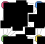
\includegraphics[width=.35\linewidth]{mc_state_transitions.pdf}
    \caption[Markov chain model of nucleotide substitutions]{
        \textbf{Markov chain model of nucleotide substitutions.}
        The evolution of characters at a site in an alignment can be modeled as a Markov chain (MC).
        The states of the MC for DNA data are the four nucleobases
        \nucleobase{A}, \nucleobase{C}, \nucleobase{G}, and \nucleobase{T}.
        The model allows transitions with rates $q_{ij}$ with $i,j \in \left\{~ A, C, G, T ~\right\}, i \neq j$ between all states,
        which correspond to substitutions of the nucleobases.
    }
    \label{fig:mc_state_transitions}
\end{figure}

% \begin{figure}[hpbt]
%  \begin{subfigure}[c]{.5\textwidth}
%     \centering
%     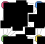
\includegraphics[width=.7\linewidth]{mc_state_transitions.pdf}
%     \caption{}
%     \label{fig:mc_state_transitions:sub:mc_chain}
%  \end{subfigure}
%  \begin{subfigure}[c]{.5\textwidth}
%     \begin{align*}
%         Q ~&=~
%          \begin{pmatrix}
%          ~-q_{A}   &   q_{AC}   &   q_{AG}   &   q_{AT}~~ \\
%          ~q_{CA}   &  -q_{C}    &   q_{CG}   &   q_{CT}~~ \\
%          ~q_{GA}   &   q_{GC}   &  -q_{G}    &   q_{GT}~~ \\
%          ~q_{TA}   &   q_{TC}   &   q_{TG}   &  -q_{T}~~
%          \end{pmatrix}
%         \\ \\
%         - q_{i} ~&=~ - \sum_{j \neq i} q_{ij}, ~ i = \left\{~ A, C, G, T ~\right\}
%     \end{align*}
%     \caption{}
%     \label{fig:mc_state_transitions:sub:matrix}
%   \end{subfigure}
%     \caption[Markov chain model of nucleotide substitutions]{
%         \textbf{Markov chain Model of Nucleotide Substitutions.}
%         The evolution of characters at a site in an alignment can be modeled as a Markov chain (MC).
%         \subref{fig:mc_state_transitions:sub:mc_chain} The states of the MC for DNA data are
%         the four nucleobases \nucleobase{A}, \nucleobase{C}, \nucleobase{G}, and \nucleobase{T}.
%         The model allows transitions between all states, which correspond to substitutions between the nucleobases.
%         \subref{fig:mc_state_transitions:sub:matrix} The instantaneous transition rates between states are given
%         by the substitution rate matrix (Q-matrix), where the rows must sum to $0$.
%     }
%     \label{fig:mc_state_transitions}
% \end{figure}

The process of state transitions is defined by the substitution rate matrix %$Q$

\begin{equation}
    \begin{align*}
        Q ~&=~
         \begin{pmatrix}
         ~-q_{A}   &   q_{AC}   &   q_{AG}   &   q_{AT}~~ \\
         ~q_{CA}   &  -q_{C}    &   q_{CG}   &   q_{CT}~~ \\
         ~q_{GA}   &   q_{GC}   &  -q_{G}    &   q_{GT}~~ \\
         ~q_{TA}   &   q_{TC}   &   q_{TG}   &  -q_{T}~~
         \end{pmatrix}
        \\ \\
        - q_{i} ~&=~ - \sum_{j \neq i} q_{ij}, ~ i \in \left\{~ A, C, G, T ~\right\}
    \end{align*}
\end{equation}

% The instantaneous transition rates between states are given
% by the substitution rate matrix (Q-matrix), where the rows must sum to $0$.
where the elements $q_{ij}$ are the \emph{instantaneous transition rates} from state $i$ to state $j$.
The rows of the $Q$-matrix have the requirement to sum to $0$,
by which the diagonal elements $q_{i}$ are defined.

The expected number of substitutions at an alignment site between two nodes of the tree
is expressed as the branch length $b$ between the nodes, and is a measure of evolutionary time $t$ between them.
Under the MC model, evolutionary time and branch length are proportional to each other
with the \emph{evolutionary rate} $r$ being their proportionality factor: $t = r \cdot b$.
Then, for a given time $t$, the \emph{transition probabilities} $p_{ij}(t)$ between states in a stationary process
are obtained by exponentiating the $Q$-matrix \cite{Yang2014}.
These probabilities are specified by the matrix

\begin{equation}
    \label{ch:Foundations:sec:MLTreeInference:eq:P_matrix}
    P(t) = e^{Qt}
\end{equation}

For positive transition rates $q_{ij} > 0, \forall i \neq j$, if the process runs long enough,
the Markov chain eventually reaches the unique \emph{stationary} distribution $\Pi = (\pi_A$, $\pi_C$, $\pi_G$, $\pi_T )$,
with $\pi_i$ being the proportion of time spent in state $i$.
If the Markov process reached equilibrium after running long enough,
it can be interpreted as having generated the sequences of the MSA.
In that case, $\Pi$ is the \emph{equilibrium base composition} of the MSA,
and $\pi_i$ are the \emph{equilibrium} or \emph{stationary base frequencies} of the MSA.

\paragraph{Time-Reversible Models}
\label{ch:Foundations:sec:MLTreeInference:sub:ModelsOfSeqEvol:par:TimeReversibleModels}

As mentioned before, most models of DNA evolution assume a \emph{time-reversible} Markov process,
which means that $\pi_{i} q_{ij} = \pi_{j} q_{ji} ~ \forall \, i \neq j$.
This assumption is biologically not meaningful, as evolution is a process in time, and thus does have a direction.
It however allows for simplified calculations:
The $Q$-matrix of a time-reversible model can be formulated as the product of
a symmetric rate matrix $R = \left\{ r_{i \leftrightarrow j} \right\}$ and
a diagonal matrix with the stationary base frequencies:

\begin{align}
    \newcommand{\lra}{\leftrightarrow}
    Q = R \cdot diag(\pi_i) =
    \begin{pmatrix}
         -q_A                       &   r_{A \lra C} \cdot \pi_C   &   r_{A \lra G} \cdot \pi_G   &   r_{A \lra T} \cdot \pi_T~~  \\
        ~r_{A \lra C} \cdot \pi_A   &   -q_C                       &   r_{C \lra G} \cdot \pi_G   &   r_{C \lra T} \cdot \pi_T~~  \\
        ~r_{A \lra G} \cdot \pi_A   &   r_{C \lra G} \cdot \pi_C   &   -q_G                       &   r_{G \lra T} \cdot \pi_T~~  \\
        ~r_{A \lra T} \cdot \pi_A   &   r_{C \lra T} \cdot \pi_C   &   r_{G \lra T} \cdot \pi_G   &   -q_T
    \end{pmatrix}
\end{align}

The matrix describes the most general model of DNA evolution,
where all \num{6} substitution rates $r_{i \leftrightarrow j}, i \neq j$ and
all \num{4} base frequencies $\pi_i$ can be different.
This model is called the Generalized Time-Reversible (\toolname{GTR}) model \cite{Tavare1986}.
As the sum of the base frequencies must be $1$,
and as the substitution rates are usually normalized by requiring that $r_{G \leftrightarrow T} = 1.0$,
the \toolname{GTR} model has a total of \num{8} free parameters
(that is, \num{3} base frequencies, and \num{5} substitution rates).
The base frequencies can also be estimated from the character frequencies in the given MSA,
in which case they are called the \emph{empirical} base frequencies.

There are also more restrictive models, which have fewer free parameters,
and are thus more robust if data for estimating them is sparse, at the expense of descriptiveness.
The Jukes-Cantor model (\toolname{JC69}) \cite{Jukes1969} has no free parameter
and assumes equal substitution rates $r_{i \leftrightarrow j} = 1$, $i \neq j$
and equal base frequencies $\pi_i = \sfrac{1}{4}$.
The \toolname{K80} model \cite{Kimura1980} adds a free parameter $\kappa$,
which describes the ratio between two types of substitutions that are not equally likely to occur in evolution:
$r_{A \leftrightarrow C} = r_{G \leftrightarrow T} = \kappa \cdot r_{A \leftrightarrow G} =
\kappa \cdot r_{A \leftrightarrow T} = \kappa \cdot r_{C \leftrightarrow G} = \kappa \cdot r_{C \leftrightarrow T}$.
% \todo{if transition vs transversion was added earlier, add it here, too!}
The \toolname{F81} model \cite{Felsenstein1981} instead extends the JC69
by allowing different base frequencies: $\pi_A \neq \pi_C \neq \pi_G \neq \pi_T$.
The \toolname{HKY85} model \cite{Hasegawa1985} combines the \toolname{K80} model and the \toolname{F81} model,
and hence has \num{4} free parameters.
Further models have also been proposed, which offer compromises
between the number of free parameters and the expressiveness of the model \cite{Yang2014}.

The state space of the Markov process becomes significantly larger for protein data,
as it needs to comprise \num{20} standard amino acids instead of \num{4} nucleobases.
Hence, the \toolname{GTR} model for protein data has $(400 - 20) / 2 - 1 + 19 = 208$ free parameters.
Typical amino acid alignments do not contain enough data to reliably estimate these parameters,
and thus easily lead to over-fitting.
Thus, so-called \emph{empirical} amino acid models are commonly used,
which have substitution rates and equilibrium base frequencies
that were pre-estimated on large collections of reference alignments.
Among others, some popular models include \toolname{DAYHOFF} \cite{Dayhoff1978},
\toolname{WAG} \cite{Whelan2001}, and \toolname{LG} \cite{Le2008}.

% ======================================================================================================================
%     Further Aspects of Tree Inference
% ======================================================================================================================

\subsection{Further Aspects of Tree Inference}
\label{ch:Foundations:sec:MLTreeInference:sub:FurtherAspects}

Evolution is an incredibly complex process with intricate details.
Many more models and methods have thus been proposed to refine tree inference \cite{Yang2014},
of which we here briefly introduce a few.
% For understanding the methods described in this work, the above introduction should suffice.
% For the distinguished reader, we here still mention a few other aspects that are related to the topic.
% While a detailed description of these models and methods is not necessary for understanding the main chapters of this work,
% we here still mention a few other related aspects.

\paragraph{Rate Heterogeneity}
\label{ch:Foundations:sec:MLTreeInference:sub:FurtherAspects:par:RateHeterogeneity}

The models of sequence evolution described above make the simplifying assumption
that the alignment sites evolve independently and are identically distributed.
However, certain regions of DNA or amino acid sequences are under higher evolutionary pressure than others,
for example if they describe important molecular functions that are conserved in their evolutionary history.
It is thus expected that some alignment sites evolve faster than others.
That is, the evolutionary rate $r$ of these sites is not constant across the alignment.
In the context of phylogenetic inference,
several models of \emph{rate heterogeneity among sites} have been proposed to account for this,
some of which are described in the following.

A simple model is the \emph{proportion of invariable sites},
where the likelihood of an alignment site is influenced by a parameter $p \in [0,1]$
that describes the proportion of sites that are assumed to be identical (\emph{invariable}) across all taxa.
The more elaborate $\Gamma$ model \cite{Yang1994a} postulates a shape parameter $\alpha > 0$
which models the rate heterogeneity as a gamma distribution $\Gamma(\alpha)$.
The distribution shape ranges from exponential-like ($\alpha < 1$, high rate heterogeneity)
to normal-like ($\alpha > 10$, low rate heterogeneity).
Thus, by optimizing the single free parameter $\alpha$,
different unimodal rate heterogeneity profiles can be approximated.
The \toolname{CAT} or \emph{per-site rates} model \cite{Stamatakis2006a}
is a compute- and memory-efficient approximation of the $\Gamma$ model,
which explicitly assigns one of $K$ rate categories to each alignment site instead of using a distribution of rates.
Lastly, the \toolname{FreeRate} model \cite{Yang1995} allows for multimodal distributions
by using $K$ rate categories and respective weights,
which can approximate any distribution at the cost of having to estimate these free parameters.

\paragraph{Alignment Partitioning}
\label{ch:Foundations:sec:MLTreeInference:sub:FurtherAspects:par:AlignmentPartitioning}

Apart from the evolutionary rate $r$, also the substitution patterns among the sites of an MSA can differ.
In order to account for this, the MSA can be split into different \emph{partitions},
where each such partition is assigned its own model of evolution.
For example, as three nucleobases code for one amino acid in regions that encode for proteins
(see \secref{ch:Foundations:sec:EvolutionGenetics}),
three partition can be used, each modeling the evolution of the first, second, and third nucleobase of each amino acid.
Furthermore, large multi-gene MSAs can be split into partitions corresponding to individual genes,
which might be under different evolutionary pressure each.

\paragraph{Constrained Trees}
\label{ch:Foundations:sec:MLTreeInference:sub:FurtherAspects:par:ConstrainedTrees}

The tree search (see \secref{ch:Foundations:sec:MLTreeInference:sub:TreeSearch})
can (theoretically) yield any topology from the vast space of possible trees.
It is however often serviceable to run a \emph{constrained} tree search,
for example to include prior knowledge about the taxa,
to maintain congruence with a given taxonomy, or because some other constraints are required.
Such a constraint can for example be specified by enforcing certain bipartitions to be retained in the tree,
that is, splits of the taxa that must be separated from each other in the tree.
As a bipartition is induced by a branch in the tree,
this is equivalent to starting the tree search with a multifurcating tree,
and then resolving these multifurcations without changing the other parts of the tree.
A constrained search yields a \emph{constrained tree}.

% Not needed:
% Alignment Partitioning

% ======================================================================================================================
%     Likelihood Computation
% ======================================================================================================================

\subsection{Likelihood Computation}
\label{ch:Foundations:sec:MLTreeInference:sub:LikelihoodComputation}

We here introduce the basic computational aspects of the Maximum Likelihood method.
For a more exhaustive description of the topic, see \cite{Yang2014}.
We assume a fixed tree topology $T$, fix branch lengths $\bar{b}$,
as well as a given model of sequence evolution $M$ with parameters $\bar{\theta}$.
That is, we do not cover the tree search itself here,
% \secref{ch:Foundations:sec:MLTreeInference:sub:TreeSearch}
but describe how to compute the likelihood $\mathcal{L}$
(\eqnref{ch:Foundations:sec:MLTreeInference:eq:likelihood}) for a given MSA under these conditions.

A central point of the ML method is to account for the unknown states at the inner nodes of the tree.
That is, the total likelihood is obtained by summing over the probabilities of every possible state of the inner nodes,
which can be efficiently computed by the \emph{Felsenstein pruning algorithm} (FPA) \cite{Felsenstein1981}.
It traverses the tree in post-order fashion, that is from the tips towards the (virtual) root,
and recursively calculates a so-called \emph{conditional likelihood vector} (CLV) at each inner node.

In a sense, a CLV summarizes the subtree below its corresponding node.
For every alignment site and every state,
it describes the \emph{conditional likelihood} of the node to be in that state at that site,
given the subtree topology and its branch lengths, for the respective subset of the alignment (tip sequences).
We here assume a set $N$ of states, that is, the sequences consist of characters $c \in N$,
for example $N = \left\{~ \nucleobase{A}, \nucleobase{C}, \nucleobase{G}, \nucleobase{T} ~\right\}$.
Furthermore, for simplicity, we do not consider alignment partitioning or rate heterogeneity among sites here,
and thus use a fixed evolutionary rate $r$.
Then, a CLV contains $|N|$ elements per alignment site,
each describing the conditional likelihood of being in the corresponding state.
For DNA data, these are CL(\nucleobase{A}), CL(\nucleobase{C}), CL(\nucleobase{G}), and CL(\nucleobase{T}).

\paragraph{Felsenstein Pruning Algorithm}
\label{ch:Foundations:sec:MLTreeInference:sub:LikelihoodComputations:par:FPA}

In order to start the recursion of the FPA, first, the CLVs at the tip nodes have to be initialized.
In principle, these can be the actual likelihoods of observing the characters $c \in N$ at the corresponding site.
However, this uncertainty is rarely available in empirical data.
Thus, tip nodes are usually initialized with ``pseudo-CLVs'',
where for instance a nucleobase \nucleobase{A} in the alignment yields
CL(\nucleobase{A}) $= 1$, and CL(\nucleobase{C}) $=$ CL(\nucleobase{G}) $=$ CL(\nucleobase{T}) $= 0$.

\begin{figure}[pthb]
    \centering
    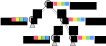
\includegraphics[width=.85\linewidth]{clv_fpa.pdf}
    \caption[Felsenstein pruning algorithm]{
        \textbf{Felsenstein pruning algorithm.}
        An exemplary tree topology with a (virtual) root {\sffamily R}, an inner node {\sffamily V},
        and three other nodes {\sffamily U}, {\sffamily L}, and {\sffamily M},
%         (which can be either tips or inner nodes),
        and branch lengths between nodes.
        Potential subtrees are marked by triangles below nodes.
%         For the recursive computation during Felsenstein's pruning,
%         Because of the recursive nature of the algorithm,
%         it is irrelevant whether the last three nodes are tips or have subtrees (marked here by triangles below them).
        \\
        Each node has a CLV assigned to it, which ``summarizes'' the subtree below it.
        A CLV stores a conditional likelihood for every alignment site and for every state.
        Here, for simplicity, we show the CLVs for one site and for four states,
        which for instance represent the likelihood of that site to be in either state of the four nucleobases.
        %\nucleobase{A}, \nucleobase{C}, \nucleobase{G}, and \nucleobase{T}.
%         Lastly, the branches of the tree have branch lengths assigned to them.
    }
    \label{fig:clv_fpa}
\end{figure}

After the tip CLVs have been initialized, the algorithm traverses up the tree, see \figref{fig:clv_fpa}.
This can be thought of as moving along the branches towards a parent node,
which induces the possibility of state transitions.
This step is thus where the model $M$ is employed (see \secref{ch:Foundations:sec:MLTreeInference:sub:ModelsOfSeqEvol}).
As we assumed a fixed evolutionary rate $r$,
we can infer the time $t$ between two nodes from the branch length $b$ between them: $t = r \cdot b$.
% Then, in order to compute the likelihood of state changes while moving from a child node to its parent,
% the model $M$ is employed, as explained in \secref{ch:Foundations:sec:MLTreeInference:sub:ModelsOfSeqEvol}.
% In particular,
Then, for a given branch, we can compute the probability $p_{ij}(t)$ of a transition
from state $i$ to state $j$ after moving along the branch, see \eqnref{ch:Foundations:sec:MLTreeInference:eq:P_matrix}.
Note that the probability $p_{ij}$ depends on the branch length,
meaning that for every branch (and every update in its branch length during optimization,
see \secref{ch:Foundations:sec:MLTreeInference:sub:BLO}),
a separate $P$-matrix has to be computed from the $Q$-matrix of the model.

At a parent node whose children have been computed, we can now apply the recursion step of the algorithm.
For instance, in the topology shown in \figref{fig:clv_fpa}, the CLV of an inner node {\sffamily V}
can be computed given its children {\sffamily L} and {\sffamily M}.
For the computation, the CLVs of the two child nodes,
as well as the transition probabilities $p_{ij}$ for the branch lengths $b_{LV}$ and $b_{MV}$
of the branches towards the parent are needed.
% and the respective branch lengths $b_{LV}$ and $b_{MV}$.
Then, a single entry of the CLV, that is,
the conditional likelihood of node {\sffamily V} to be in state $c$ at site $s$, is

\begin{equation}
    \label{ch:Foundations:sec:MLTreeInference:eq:CLV}
%     \mbox{CLV} =
    \mbox{CLV}^{(V)}_{s,c} =
    \left(~ \sum_{j \in N} p_{cj}(r \cdot b_{LV}) \cdot \mbox{CLV}^{(L)}_{s,j} \right)
    \left(~ \sum_{k \in N} p_{ck}(r \cdot b_{MV}) \cdot \mbox{CLV}^{(M)}_{s,k} \right)
\end{equation}

The equation can be interpreted as follows:
The product of transition probability and conditional likelihood represents a change from state $c$ to another state in $N$.
By summing this product for all states, all possible inner states are accounted for.
Finally, the product of the two sums is the new conditional likelihood of the node being in state $c$ at site $s$,
given the evolutionary history of its children and their subtrees.

By repeating the computation for every state $c \in N$ and every site $s$ of the alignment,
the complete CLV for node {\sffamily V} is computed.
The recursion is then applied to all nodes upwards the tree, until all CLVs are computed.

\paragraph{Likelihood Evaluation at the Root}
\label{ch:Foundations:sec:MLTreeInference:sub:LikelihoodComputations:par:RootLikelihood}

Once all CLVs are computed, the overall likelihood $\mathcal{L}$ can be computed from the CLV of the root node.
Given the root node {\sffamily R} as shown in \figref{fig:clv_fpa},
the total \emph{per-site likelihood} $\mathcal{L}_s$ of an alignment site $s$ is
accumulated from the conditional likelihoods of all states,
taking their respective base frequencies $\pi_i$ into account:

\begin{equation}
    \label{ch:Foundations:sec:MLTreeInference:eq:root_site_likelihood}
    \mathcal{L}_{s} = \sum_{i \in N} \pi_i \cdot \mbox{CLV}^{(R)}_{s,i}
\end{equation}

Due to the time reversibility of the model, for unrooted trees, a \emph{virtual} root can be used,
that is, an additional node that is presumed to be present on a branch of the tree.
% The calculation is invariant to the exact position of this node along the branch.
% which might coincide with an actual node of the tree
If for example the node {\sffamily R} in \figref{fig:clv_fpa} represents a virtual root,
the two branches between nodes {\sffamily U} and {\sffamily V}
are actually one branch with branch length $b_{UV} = b_{UR} + b_{VR}$.
Then, an alternative way of computing the per-site likelihood is what we here call the (per-site) \emph{edge likelihood}.
Instead of using the CLV at the virtual root {\sffamily R}, we can use the CLVs of {\sffamily U} and {\sffamily V},
and the corresponding branch length $b_{UV}$ for the computation.
In that case, state transitions along the branch have to be additionally accounted for in the computation.
The per-site edge likelihood of an alignment site $s$ can then be computed as

\begin{equation}
    \label{ch:Foundations:sec:MLTreeInference:eq:edge_likelihood}
    \mathcal{L}_{s} = \sum_{i \in N} \sum_{j \in N} \pi_i \cdot \mbox{CLV}^{(U)}_{s,i} \cdot
    p_{ij}(r \cdot b_{UV}) \cdot \mbox{CLV}^{(V)}_{s,j}
\end{equation}

This way of calculating the edge likelihood $\mathcal{L}_s$ works for any two adjacent nodes,
if their respective CLVs have been computed to represent the two subtrees induced by the branch between the nodes.

Finally, the overall likelihood $\mathcal{L}( \mbox{MSA} ~|~ T, \bar{b}, M, \bar{\theta} )$
for the entire MSA can be computed.
For mathematical simplicity, the sites are generally assumed to evolve independently,
although this is not expected to be the case from a biological perspective.
Then, for an alignment with $m$ sites, the overall likelihood is simply the product of the per-site or edge likelihoods:

\begin{equation}
    \label{ch:Foundations:sec:MLTreeInference:eq:root_likelihood}
    \mathcal{L} = \prod_{s=1}^{m} \mathcal{L}_s
\end{equation}

For computational reasons, and to avoid numerical underflow, in practice,
the logarithm of the likelihood (\emph{log-likelihood}) is typically used.
Furthermore, as identical sites yield exactly the same likelihood,
such sites are often compressed and the respective likelihood is multiplied with an according \emph{weight}.
% Lastly, we note that the derivatives of the above likelihood functions can be obtained analytically \cite{Yang2014},
% which is needed for optimizing the branch lengths,
% as explained in \secref{ch:Foundations:sec:MLTreeInference:sub:TreeSearch}.

% ======================================================================================================================
%     Branch Length Optimization
% ======================================================================================================================

\subsection{Branch Length Optimization}
\label{ch:Foundations:sec:MLTreeInference:sub:BLO}

Another important aspect of the tree search
is the optimization of the branch lengths of the tree.
That is, for a given tree topology $T$, and a fixed model $M$ with parameters $\bar{\theta}$,
we want to compute the branch lengths $\bar{b}$
that maximize the likelihood $\mathcal{L}( \mbox{MSA} ~|~ T, \bar{b}, M, \bar{\theta} )$.
This procedure is called \emph{branch length optimization} (BLO),
and typically uses the Newton-Raphson method \cite{Ypma1995},
as mentioned in \secref{ch:Foundations:sec:MLTreeInference:sub:TreeSearch}.

We consider to optimize a single branch length $b$.
In order to maximize $\mathcal{L}$, we need to find the root of the first derivative $\mathcal{L}'$.
The Newton-Raphson method takes an initial value for $b$ and then
iteratively approximates values that lead closer to the root:

\begin{equation}
    \label{ch:Foundations:sec:MLTreeInference:eq:BLO}
    b_{n+1} = b_n - \frac{ \mathcal{L}' }{ \mathcal{L}'' }
\end{equation}

Note that the derivatives $\mathcal{L}'$ and $\mathcal{L}''$ can be obtained analytically \cite{Yang2014},
and have to be computed in every iteration.
The algorithm stops when the change in $b$ between two iterations is below a threshold,
that is, when then optimization \emph{converges}.
This procedure is repeated for all branch lengths $\bar{b}$ in the tree.

% ######################################################################################################################
%         Phylogenetic Placement
% ######################################################################################################################

\section{Phylogenetic Placement}
\label{ch:Foundations:sec:PhylogeneticPlacement}

In studies of sequence data, one of the most common tasks is a phylogenetic analysis of the data,
that is, to infer the evolutionary context of the sequences.
However, since the amount of sequence data produced in typical metagenomic studies can be quite substantial,
computational challenges and bottlenecks arise \cite{Scholz2012}.
In particular, both calculating an MSA and inferring a phylogeny are NP-hard \cite{Just2001,Chor2005},
and thus impractical or infeasible for large datasets.
Furthermore, metagenomic reads are often short, and hence lack phylogenetic signal
to robustly infer a tree and to properly resolve their relationships.

Thus, \emph{phylogenetic placement}, also called \emph{evolutionary placement},
has been developed for conducting phylogenetic analyses of such data,
as implemented in tools such as
\toolname{pplacer} \cite{Matsen2010}, \toolname{RAxML-EPA} \cite{Berger2011}, and \toolname{EPA-ng} \cite{Barbera2018}.
% cited more than 630 times (as of 2018-07-01)
Instead of resolving the phylogeny of a set of metagenomic sequences,
phylogenetic placement treats each sequence, called a \emph{\acl{QS}}\acused{QS} (\acs{QS}), separately.
It evaluates how these \acp{QS} relate to an existing \emph{\acl{RT}}\acused{RT} (\acs{RT}) based on known reference sequences.
For each \ac{QS}, it computes the probabilities of \emph{placing} the sequence on the branches of the \ac{RT},
% In other words, it maps the \acp{QS} of interest onto the branches of an \ac{RT},
thereby classifying them into a phylogenetic context of related sequences,
without the need to resolve relationships between the \acp{QS}.

Phylogenetic placement can be carried out if the \acp{QS} can be aligned to the alignment of the reference sequences.
In the most common use case, the \acp{QS} are reads or amplicons from environmental samples.
Most often barcoding regions or marker genes such as 16S or 18S are used
(see \secref{ch:Foundations:sec:SequenceAnalysis:sub:Metagenomics}),
but there also exist studies that use different, or even a set of, maker genes \citep{Sunagawa2013a}.
Furthermore, other types of sequences such as \textsubscript{mi}tags \citep{Logares2014} can be used.

The \ac{RT} and the reference sequences it represents are typically assembled by the user
so that they capture the expected species diversity in the samples.
We however proposed an automated approach for assembling suitable sets of reference sequences \cite{Czech2018},
which we describe in \chpref{ch:AutomaticTrees}.
Distinct samples from one study are typically placed on the same underlying \ac{RT}
in order to facilitate comparisons between the samples,
see \secref{ch:Foundations:sec:PhylogeneticPlacement:sub:ExistingMethods}.
% Such a mapping also elucidates the evolutionary distance between the query and the reference sequences,
% see \secref{ch:Foundations:sec:PhylogeneticPlacementAnalysis:sub:Distances}.

% The result of phylogenetic placement is a mapping of the query sequences to the branches of the reference tree.
% In brief, phylogenetic placement calculates the most probable insertion branches for each given \acf{QS} on a \acf{RT}.

% In short, for a given \acf{QS}, phylogenetic placement computes a mapping of the \ac{QS}
% to the most closely related branches of a fixed \acf{RT} based on known reference sequences.
% Phylogenetic placement uses a fixed \acf{RT} based on known reference sequences to compute a mapping
% of \acfp{QS} to the branches of the tree that are most closely related to the \ac{QS}.
% This mapping classifies the \acp{QS} (e.g., sequences from a metagenomic study) into a phylogenetic context

% ======================================================================================================================
%     Pipeline and Computation
% ======================================================================================================================

\subsection{Pipeline and Computation}
\label{ch:Foundations:sec:PhylogeneticPlacement:sub:PipelineAndComputation}

% \todo{pipeline diagram, data flow, etc, reference to chapters?!}

% \paragraph{Preparation}
% \label{ch:Foundations:sec:PhylogeneticPlacement:sub::par:Preparation}

We here assume to have given a set of suitable reference sequences, their alignment, and an \ac{RT} inferred from them.
As phylogenetic placement used a maximum likelihood criterion, the \ac{RT} has to be strictly bifurcating.
Prior to the placement, the \acp{QS} need to be aligned against the reference alignment of the \ac{RT}
by programs such as \toolname{PaPaRa} \cite{Berger2011a,Berger2012} or \toolname{hmmalign} \cite{Eddy1998,Eddy2009},
see also \secref{ch:Foundations:sec:SequenceAnalysis:sub:SequenceAlignment}.
The input to phylogenetic placement are then the \acf{RT}, its underlying alignment, and the aligned \acfp{QS}.

\paragraph{Computation for one Query Sequence}
\label{ch:Foundations:sec:PhylogeneticPlacement:sub:PipelineAndComputation:par:ComputingQuerySequence}

% The placement is then conducted for each \ac{QS} separately
% by initially inserting a \ac{QS} as a new tip into a branch of the tree,
% then re-optimizing the branch lengths that are most affected by the insertion,
% and thereafter evaluating the resulting likelihood score of the tree.
% The \ac{QS} is then removed from the current branch and subsequently placed into all other branches of the \ac{RT}.

The placement is conducted for each \ac{QS} separately, always using the same fixed \ac{RT} as a starting point.
Each branch of the tree is evaluated as a potential \emph{placement location} of the \ac{QS},
which indicates how likely the branch is to be the ancestor of the \ac{QS}.
In \figref{fig:tiny_tree},
the procedure for one \ac{QS} and one branch (between nodes {\sffamily D} and {\sffamily P}) is shown:
The sequence is inserted as a new tip node {\sffamily Q} on the branch,
connected to it by a new \emph{pendant} branch and a new node {\sffamily C}.
This splits the original branch into two parts, called the \emph{distal} and the \emph{proximal} branch, respectively,
which are named according to the direction of the root of the tree.
Note that the tree can also be unrooted, in which case a top-level trifurcation is typically used as root.

\begin{figure}[pthb]
    \centering
    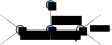
\includegraphics[width=.7\linewidth]{tiny_tree.pdf}
    \caption[Terminology of a phylogenetic placement]{
        \textbf{Terminology of a phylogenetic placement.}
        The nodes {\sffamily D} and {\sffamily P} belong to the reference tree (RT).
        When placing a query sequence (QS), the branch between them %{\sffamily D} and {\sffamily P}
        is split into two parts by a new node {\sffamily C},
        which serves as the attachment point for another new node {\sffamily Q} that represents the QS.
        The \emph{pendant} branch leads to {\sffamily Q}.
        The original branch is split into the \emph{proximal} branch, which leads towards the root of the RT,
        and the \emph{distal} branch, which leads away from the root.
    }
    \label{fig:tiny_tree}
\end{figure}

In the next step, the branch lengths of the tree are optimized,
as explained in \secref{ch:Foundations:sec:MLTreeInference:sub:BLO}.
After the optimization, the sum of the lengths of the distal and proximal branches is not necessarily equal
to the original branch length between {\sffamily D} and {\sffamily P}.
Thus, typically, the two lengths are proportionally rescaled to maintain this equality.

Lastly, the likelihood of the tree with the newly attached sequence is evaluated
as explained in \secref{ch:Foundations:sec:MLTreeInference:sub:LikelihoodComputation}.
Note that the likelihood computation uses the MSA (extended by the query sequence),
the tree topology and branch lengths, as well as the model and its parameters as before.
The model of nucleotide evolution should be the same that was used when inferring the tree,
see \secref{ch:Foundations:sec:MLTreeInference:sub:ModelsOfSeqEvol}.
% mention that epa ng can use all the model stuff explaine above: subst models, rate hetero, etc
After this, the newly created nodes on the branch are removed again, thus restoring the original reference tree.

The above procedure is repeated for every branch $i$ of the tree $T$,
yielding a set of likelihood scores $\mathcal{L}(i)$ for each possible placement location.
Thus, for each branch of the tree, the process yields a so-called \emph{placement} of the \ac{QS},
that is, an optimized position on the branch, along with a likelihood score for the whole tree.
The likelihood scores for a \ac{QS} are then transformed into probabilities,
which quantify the uncertainty of placing the sequence on the respective branch \cite{Strimmer2002,VonMering2007}.
The probability of placing a \ac{QS} on a branch $q$ is called the \emph{\acl{LWR}}\acused{LWR} (\acs{LWR}),
and is calculated relative to the other branches $i$ of the tree $T$ as

\begin{equation}
    \label{ch:Foundations:sec:PhylogeneticPlacement:eq:LWR}
    \mbox{LWR}(q) =  \frac{ \mathcal{L}( q )}{ \sum_{i \in T} \mathcal{L}( i )}
\end{equation}

By construction, the sum of the \acp{LWR} of all branches for a single \ac{QS} is $1.0$.
It can thus be interpreted as a probability distribution over the branches of the tree,
as shown in \figref{fig:tree_epa}.
For most use cases, the \acp{LWR} and the respective placement on the branches are the most important values,
while pendant lengths are rarely used in downstream analyses.
However, long pendant lengths can indicate that the \ac{RT} is missing sequences that are closely related to the \ac{QS}.

\begin{figure}[hpbt]
    \centering
    \includegraphics[width=.6\linewidth]{pppp/tree_epa.pdf}
    \caption[Phylogenetic Placement of a Query Sequence]{
        \textbf{Phylogenetic Placement of a Query Sequence.}
        Each branch of the reference tree is tested as a potential insertion position, called a \emph{placement}
        (blue dots; pendant lengths are ignored here).
        Note that placements have a specific position on their branch, due to the branch length optimization process.
        A probability of how likely it is that the sequence belongs to a specific branch is computed
        (numbers next to dots),
        which is called the \emph{likelihood weight ratio} (LWR).
%         based on the maximum likelihood score of the whole tree. %(that is, including the query sequence)
        The bold number (0.7) denotes the most probable placement of the sequence.
    }
    \label{fig:tree_epa}
\end{figure}

\paragraph{Accelerations}
\label{ch:Foundations:sec:PhylogeneticPlacement:sub:PipelineAndComputation:par:Accelerations}

The most expensive part of the placement computation are the branch lengths optimizations.
Thus, several techniques have been developed to accelerate the placement process \cite{Barbera2018}.

Firstly, above, all branches of the tree were optimized when evaluation a placement location,
which gives the most accurate results.
In practice however, it suffices to only optimize the three branches of the placement location
without losing too much accuracy.

Secondly, because the reference tree is fixed (except for the newly created nodes),
the CLVs of all possible subtrees can be precomputed,
which drastically accelerates the likelihood evaluation.
Using \figref{fig:tiny_tree} as an example,
with two CLVs of the nodes {\sffamily D} and {\sffamily P}, and one application of the Felsenstein Pruning Algorithm
(see \secref{ch:Foundations:sec:MLTreeInference:sub:LikelihoodComputations:par:FPA}),
the CLV of node {\sffamily C} can be computed.
Then, the final likelihood can be evaluated as the edge likelihood of the pendant edge,
using this CLV as well as the pseudo-CLV of node {\sffamily Q}.

Thirdly, further acceleration can be achieved with a \emph{pre-placement} heuristic:
A first approximate evaluation of a placement location can be conducted by using
distal and proximal lengths based on the respective original branch length of the tree, and a fixed default pendant length.
Then, only the most likely fraction of locations is thoroughly evaluated, that is, including branch length optimizations.
This way, millions or even billions of sequences can be placed within acceptable time \cite{Barbera2018}.
This is however a heuristic that might lead to suboptimal results by ignoring placement locations
whose \ac{LWR} is significantly improved by the branch length optimization process.
If the \ac{RT} is however well suited for the \acp{QS}, this situation is generally not expected to occur.

\paragraph{Placement Result}
\label{ch:Foundations:sec:PhylogeneticPlacement:sub:PipelineAndComputation:par:PlacementResults}

The placement process is repeated independently for every \ac{QS}.
That is, for each \ac{QS}, the algorithm starts calculating placements from scratch on the original \ac{RT}.
The result thus classifies each \ac{QS} in the phylogenetic context of the \ac{RT},
without resolving the evolutionary relationships between the \acp{QS}.

The data is usually stored in so-called \fileformat{jplace} files \cite{Matsen2012},
which is a standard based on the \fileformat{JSON} format \cite{JsonMemo,JsonStandard}.
It stores the \ac{RT} in \fileformat{Newick} format, including tip names and branch lengths,
and extended by a post-order numbering of the edges to be referenced by the placements.
The main part of the file is a list of lists:
For each \ac{QS}, its list of placements is stored.
A placement is described by its edge number (referencing the \ac{RT}),
the \ac{LWR}, the pendant length, and the distal length.
The proximal length is usually omitted, as it can be inferred from the branch length of the tree.
Furthermore, the format can summarize multiple identical \acp{QS}
by allowing several names for each list of placements,
where each name can also have a weight (called its \emph{multiplicity}).
Lastly, usually not all placement locations are stored in the file,
as the ones with low \ac{LWR} do not contribute much to post-analysis methods anyway.

% In summary, the result of a phylogenetic placement analysis is a mapping of the \acp{QS} in a sample
% to positions on the branches of the \ac{RT}.
% Each such position, along with the corresponding \ac{LWR}, is called a placement of the \ac{QS}.
% The result of phylogenetic placement is a mapping of each \ac{QS} (e.g., environmental reads)
% to positions on the branches of the \ac{RT}, amended by probabilities in form of their likelihood weight ratios.
% Each \ac{QS} is thus represented by its placement positions, which are also called its placements.
% along with the respective likelihood weight ratios.f

% Each such sample represents a geographical location, a body site, a point in time, etc.
% In the following, we represent a sample by the placement locations of its metagenomic \acp{QS},
% including the respective per-branch \acp{LWR}.
% Furthermore, for a specific analysis, we assume the standard use case,
% that is, all placements were computed on the same fixed \acf{RT} and \acl{RA}.

% ======================================================================================================================
%     Use Cases and Applications
% ======================================================================================================================

\subsection{Use Cases and Applications}
\label{ch:Foundations:sec:PhylogeneticPlacement:sub:UseCasesApplications}

Phylogenetic placement is a flexible tool that yields useful biological information \emph{per se},
but that also can be utilized for a variety of downstream analyses.

\paragraph{Comparison to Existing Methods}
\label{ch:Foundations:sec:PhylogeneticPlacement:sub:UseCasesApplications:par:Comparison}

A typical task in metagenomic studies is to identify and classify the environmental sequences with respect
to known reference sequences, either in a taxonomic or phylogenetic context,
as mentioned in \secref{ch:Foundations:sec:SequenceAnalysis:sub:Metagenomics}.
Conventional methods for this task, such as \toolname{BLAST} \cite{Altschul1990}, are based on sequence similarity.
Such methods are fast, but only attain satisfying accuracy levels
if the query sequences are sufficiently similar to the reference sequences.
Furthermore, the best \toolname{BLAST} hit does often \emph{not} represent the most closely related species \cite{Koski2001}.
This is particularly true for environments where available reference databases do not exhibit
sufficient taxon coverage \citep{Mahe2017}.
Moreover, as insufficient taxon coverage cannot be detected by methods that are based on sequence similarity,
they can potentially bias downstream analyses.

More recent methods can alleviate some of these issues, for instance by
using machine learning techniques to obtain a taxonomic classification of metagenomic sequences \cite{Vervier2015},
or by utilizing a phylogeny inferred from metagenomic OTUs to classify microbial communities \cite{Tanaseichuk2014}.
However, the common shortcoming of these methods is
that they lack a way of incorporating phylogenetic information of known sequences.

A phylogenetic placement analysis \emph{does} incorporate known phylogenetic relationships,
and hence provides a more accurate means for read identification and classification.
For example, the classification of query sequences
can be summarized by means of sequence abundances \cite{Pace1997,Hugenholtz1998},
or to obtain taxonomic assignments \cite{Kozlov2016}.

However, phylogenetic placement also allows for more elaborate downstream analyses.
Firstly, the reference tree usually offers a higher resolution than simple per-taxon abundance counts,
and the amount of mapped \acp{QS} per branch can be directly visualized on the \ac{RT} \citep{Mahe2017},
as shown in \secref{ch:Visualization:sec:Motivation}.
Secondly, established methods such as Edge PCA and Squash Clustering \citep{Matsen2011a},
which we introduce in \secref{ch:Foundations:sec:PhylogeneticPlacement:sub:ExistingMethods},
allow for identifying subtle differences between distinct samples,
thus enabling comparative studies directly based on phylogenetic placement.
Lastly, we proposed novel methods for visualizing and clustering phylogenetic placement data \citep{Czech2018a},
which we describe in \chpref{ch:Visualization} and \chpref{ch:Clustering}.
Another typical task in metagenomic studies is to discover novel diversity within the samples,
which can be conducted using phylogenetic placement, as outlined in \chpref{ch:ConclusionOutlook}.

\paragraph{Variants and Derived Tools}
\label{ch:Foundations:sec:PhylogeneticPlacement:sub:UseCasesApplications:par:DerivedTools}

There also exist variants of phylogenetic placement that use maximum parsimony \cite{Berger2011}
and minimum evolution \cite{Filipski2015} instead of maximum likelihood,
and variants that calculate Bayesian posterior probabilities \cite{Matsen2010}.
The boosting method \toolname{SEPP} has been proposed to improve the accuracy of the placements \cite{Mirarab2012}.
The recently proposed tool \toolname{RAPPAS} \cite{Linard2018} is an alignment-free approach
that is not based on ML, but yields comparable results to standard phylogenetic placement implementations.

Phylogenetic placement has further been used for a variety of applications and derived pipelines, such as
species delimitation as in \toolname{PTP} \cite{Zhang2013} and \toolname{mPTP} \cite{Kapli2017},
genome and metagenome analysis as in \toolname{PhyloSift} \cite{Darling2014},
taxonomic identification and phylogenetic profiling as in \toolname{TIPP} \cite{Nguyen2014}, and
identification and correction of taxonomically mislabeled sequences as in \toolname{Sativa} \cite{Kozlov2016}.

% these tools combine 1,010 more citations (as of 2018-07-01)

% ======================================================================================================================
%     Placement Processing
% ======================================================================================================================

\subsection{Placement Processing}
\label{ch:Foundations:sec:PhylogeneticPlacement:sub:PlacementProcessing}

% \paragraph{Normalization}
% \label{ch:Foundations:sec:PhylogeneticPlacement:sub:PlacementProcessing:par:Normalization}

When placing multiple environmental samples, for instance, from different geographical locations,
typically, the same \ac{RT} is used, in order to allow for comparisons of the phylogenetic composition of these samples.
In this context, it is important to consider how to properly normalize the samples.
Normalization is required as the sample size (often also called library size),
that is, the number of sequences per sample, can vary by several orders of magnitude,
due to efficiency variations in the sequencing process or biases introduced by the amplification process,
as explained in \secref{ch:Foundations:sec:SequenceAnalysis:sub:Metagenomics}.

Selecting an appropriate normalization strategy hence constitutes a common problem in many metagenomic studies.
The appropriateness depends on data characteristics \cite{Weiss2017}, but also on the biological question asked.
For example, estimating indices such as the species richness are often implemented
via so-called \emph{rarefaction} and rarefaction curves \cite{Gotelli2001}
by randomly re-drawing sequences from the set of sequences in a sample to obtain comparable sample sizes.
This however ignores a potentially large amount of the available valid data \cite{McMurdie2014}.
Furthermore, the specific type of input sequence data has to be taken into account for normalization:
Biases induced by the amplification process can potentially be avoided if, instead of amplicons,
data based on shotgun sequencing are used, such as \textsubscript{mi}tags \cite{Logares2014}.
Moreover, similar sequences can be clustered prior to phylogenetic placement analysis, for instance,
by constructing so-called \emph{operational taxonomic units} (OTUs) \cite{Edgar2010,Mahe2014,Mahe2015,Rognes2016}.
Analyses using OTUs focus on species diversity instead of simple abundances.
OTU clustering substantially reduces the number of sequences,
and hence greatly decreases the computational cost for placement analyses.
Lastly, one may completely ignore the abundances (which correspond to the \emph{multiplicities} of placements)
of the placed sequences, reads, or OTUs, and only be interested in their presence/absence when comparing samples.

Which of the above analysis strategies is deployed,
depends on the specific design of the study and the research question at hand.
The common challenge is that the number of sequences per sample differs, which affects most post-analysis methods.

In the following, we therefore explain how the necessary normalizations of sample sizes can be performed.
We also introduce established terminology,
and describe general techniques for interpreting and working with phylogenetic placement data.
These are not methods of their own, but they are tools and building blocks
that are necessary for the analysis methods explained and introduced later.

\paragraph{Edge Masses}
\label{ch:Foundations:sec:PhylogeneticPlacement:sub:PlacementProcessing:par:EdgeMasses}

Methods that compare samples directly based on their sequences,
such as the UniFrac distance \cite{Lozupone2005,Lozupone2007a},
can benefit from rarefaction \cite{Weiss2017}.
However, in the context of phylogenetic placement, rarefaction is not necessary.
Thus, more valid data can be kept.
To this end, it is convenient to think of the reference tree as a graph.
% (when exploiting graph properties of the tree, we refer to the branches of the tree as edges).
Then, the per-branch \acp{LWR} for a single \ac{QS}
can be interpreted as mass points distributed over the edges of the \ac{RT},
including their respective placement positions on the branches, as shown in \figref{fig:tree_epa}.
We call this the \emph{mass interpretation} of the placed \acp{QS},
and henceforth use mass and \ac{LWR} interchangeably.
For simplicity, we here ignore that typically not all placements are stored in \fileformat{jplace} files,
meaning that the mass per QS can also be $<1$.
Hence, each \ac{QS} is assumed to have a total accumulated mass of $1.0$ on the \ac{RT}.
The \emph{mass of an edge} or \emph{edge mass} refers to the sum of the \acp{LWR} on that edge for all \acp{QS} of a sample,
as shown in \figref{fig:imbalance:sub:ReferenceTree}.
The \emph{total mass} of a sample is then the sum over all edge masses,
which is identical to the number of \acp{QS} in the sample,

\begin{figure}[!ht]
    \centering
    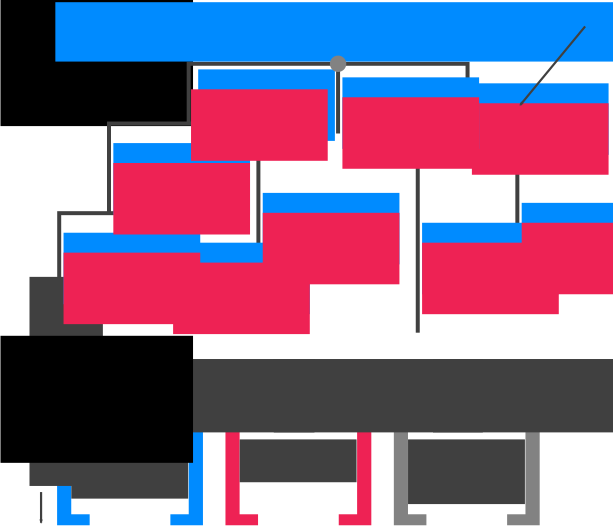
\includegraphics[width=0.8\linewidth]{imbalance.pdf}
    \begin{subfigure}{0pt}
        \phantomcaption
        \label{fig:imbalance:sub:ReferenceTree}
    \end{subfigure}
    \begin{subfigure}{0pt}
        \phantomcaption
        \label{fig:imbalance:sub:Matrices}
    \end{subfigure}
    \caption[Edge Masses and Imbalances]{
        \textbf{Edge Masses and Imbalances.}
        \subref{fig:imbalance:sub:ReferenceTree}
        Reference tree where each edge is annotated with the normalized mass (first value, blue) and
        imbalance (second value, red) of the placements in a sample.
        The imbalance is the sum of masses on the root side of the edge minus the sum of the masses on the non-root side.
        The depicted tree is unrooted, hence, its top-level trifurcation (gray dot) is used as ``root'' node.
        An exemplary calculation of the imbalance is given at the top.
        Because terminal edges only have a root side, their imbalance is not informative.
        \subref{fig:imbalance:sub:Matrices}
        The masses and imbalances for the edges of a sample constitute the rows of the first two matrices.
        The third matrix contains the available meta-data features for each sample.
        These matrices are used to calculate, for instance, the edge principal components or correlation coefficients.
    }
    \label{fig:imbalance}
\end{figure}

The key idea is to use the distribution of placement mass points over the edges of the \ac{RT} to characterize a sample.
This allows for normalizing samples of different size
by scaling the total sample mass to unit mass $1.0$.
In other words, absolute abundances are converted into relative abundances.
This way, rare species, which might have been removed by rarefaction, can be kept,
as they only contribute a negligible mass to the branches into which they have been placed.
This approach is analogous to using proportional values for methods based on OTU count tables,
that is, scaling each sample/column of the table by its sum of OTU counts \cite{Weiss2017}.
Most of the methods presented here use normalized samples, that is, they use relative abundances.
As relative abundances are compositional data, certain caveats occur \cite{Aitchison1986,Lovell2015,Gloor2016},
which we discuss where appropriate.

When working with large numbers of \acp{QS},
the mass interpretation allows to further simplify and reduce the data:
The masses on each edge of the tree can be quantized into $b$ discrete bins,
that is, each edge is divided into $b$ intervals (or bins) of the corresponding branch length.
All mass points on that edge are then accumulated into their respective nearest bin.
For example, by accumulating mass points at their nearest interval midpoint, masses are only minimally moved.
The parameter $b$ controls the resolution and accuracy of this approximation.
In the extreme case of $b:=1$, all masses on an edge are grouped into one single bin.
This \emph{branch binning} process drastically reduces the number of mass points
that need to be stored and analyzed in several methods we present,
while only inducing a negligible decrease in accuracy.
As shown in \tabref{tab:hmp_binning_error}.
branch binning can yield a speedup of up to 75\% for post-analysis run-times.

Furthermore, using masses allows to summarize a set of samples
by annotating the \ac{RT} with their average per-edge mass distribution.
This procedure, also called \emph{squashing} \cite{Matsen2011a}, sums over all sample masses per edge
and then normalizes them once more to obtain unit mass for this resulting average tree.
This normalized tree thereby summarizes the (sub-)set of samples it represents.

\paragraph{Edge Imbalances}
\label{ch:Foundations:sec:PhylogeneticPlacement:sub:PlacementProcessing:par:EdgeImbalances}

So far, we have only considered the per-edge masses.
Often, however, it is also of interest to ``summarize'' the mass of an entire clade, that is, to consider per-clade masses.
For example, sequences of the \ac{RT} that represent species or strains might not provide sufficient phylogenetic signal
for properly resolving the phylogenetic placement of short sequences \cite{Dunthorn2014}.
In these cases, the placement mass of a sequence can be spread across different edges representing the same genus or species,
thus blurring analyses based on per-edge masses.

Instead, a clade-based summary can yield clearer analysis results.
It can be computed by using the tree structure to appropriately transform the edge masses.
Each edge splits the tree into two parts
(bipartitions, see \secref{ch:Foundations:sec:TreeOfLife:sub:PhylogeneticTrees:par:TreeProperties}),
of which only one contains the root (or top-level trifurcation) of the tree.
For a given edge, its mass difference is then calculated by summing all masses in the root part of the tree
and subtracting all masses in the other part,
while ignoring the mass of the edge itself \cite{Matsen2011a}.
This difference is called the \emph{imbalance} of the edge.
It is usually normalized to represent unit total mass,
as the absolute (not normalized) imbalance otherwise propagates the effects of differing sample sizes all across the tree.
It is irrelevant where the root of the tree is,
as any re-rooting changes the sign of edge imbalance values consistently across different samples.

An example of the imbalance calculation is shown in \figref{fig:imbalance:sub:ReferenceTree}.
The edge imbalance relates the masses on the two sides of an edge to each other.
This implicitly captures the \ac{RT} topology and reveals information about its clades.
Furthermore, this transformation can also reveal differences in the placement mass distribution
of nearby branches of the tree.
This is in contrast to the KR distance
(see \secref{ch:Foundations:sec:PhylogeneticPlacement:sub:ExistingMethods:par:Distances}),
which yields low values for masses that are close to each other on the tree.
Note that for normalized samples with unit total mass,
the imbalance of a leaf edge is simply the total mass of the tree minus the mass of the edge.
It thus contains mostly irrelevant information and can often be left out.

\paragraph{Placement Data Matrices}
\label{ch:Foundations:sec:PhylogeneticPlacement:sub:PlacementProcessing:par:PlacementDataMatrices}

The edge masses and edge imbalances per sample can be summarized by two matrices,
which we use for all further downstream edge- and clade-related analyses, respectively.
In these matrices, each row corresponds to a sample, and each column to an edge of the \ac{RT}.
Note that these matrices can either store absolute or relative abundances,
depending on whether the placement mass was normalized.

Furthermore, many studies provide meta-data for their samples,
for instance, the pH value or temperature of the samples' environment.
Such meta-data features can also be summarized in a per-sample matrix, where each column corresponds to one feature.
The three matrices are shown in \figref{fig:imbalance:sub:Matrices}.
Quantitative meta-data features are the most suitable for computational purposes,
as they can be used to detect correlations with the placement mass distributions of samples.

% ======================================================================================================================
%     Existing Analysis Methods
% ======================================================================================================================

\subsection{Existing Analysis Methods}
\label{ch:Foundations:sec:PhylogeneticPlacement:sub:ExistingMethods}

\paragraph{Distance between Samples}
\label{ch:Foundations:sec:PhylogeneticPlacement:sub:ExistingMethods:par:Distances}

motivate: moving along the branches means distance between things.

kr distance. ref to nh distance?!
\cite{Evans2012}

\paragraph{Squash Clustering}
\label{ch:Foundations:sec:PhylogeneticPlacement:sub:ExistingMethods:par:SquashClustering}

squash clustering
\cite{Matsen2011a,Evans2012}


\paragraph{Edge PCA}
\label{ch:Foundations:sec:PhylogeneticPlacement:sub:ExistingMethods:par:EdgePCA}

For example, Edge principal components analysis (Edge PCA) \cite{Matsen2011a}
is a method that utilizes the imbalance matrix to detect and visualize edges
with a high heterogeneity of mass difference between samples.
Edge PCA further allows to annotate its plots with meta-data variables, for instance, by coloring,
thus establishing a connection between differences in samples and differences in their meta-data \cite{Srinivasan2012}.

edge pca
\cite{Matsen2011a,Evans2012}

we use these methods repeatedly to compare our novel methods to.

% ######################################################################################################################
%         PhAT
% ######################################################################################################################

\chapter{Phylogenetic Automatic (Reference) Trees}
\label{ch:AutomaticTrees}

\paperbox{
    This chapter is based on the peer-reviewed publication:
}{\paperart}{
    \textbf{Contributions:} Lucas Czech... Pierre Barbera... Alexandros Stamatakis... and...
}

% ######################################################################################################################
%     Motivation
% ######################################################################################################################

\section{Motivation}
\label{ch:AutomaticTrees:sec:Motivation}

Phylogenetic placement is particularly helpful for studying new, unexplored environments,
for which no closely related sequences exist in reference databases (e.g., \citealp{Mahe2017}).
However, the selection of suitable reference sequences for inferring the \ac{RT} constitutes
a challenge for studying such environments, as this typically is a manual process.
Furthermore, conducting phylogenetic placement requires a higher computational effort
with respect to the placement algorithms \emph{per se}, but also the pre- and post-processing,
than, for instance, similarity based methods.
Due to the continuous advances in molecular sequencing, existing placement methods
as well as respective pre- and post-processing tools have already reached their scalability limits.
% Another limitation is the selection process of reference sequences.

% Evolutionary Placement can be used for taxonomic assignment.
% In studies that specifically look for certain kinds of organisms,
% e.g, protists \citep{Mahe2017},
% it usually suffices to use a taxonomy covering the organisms of interest,
% potentially including outgroups from more distance species.
% As metagenomic analyses get cheaper,
% it is however to be expected that researchers want to target more than one group of organisms within one study.
% Thus, this limitation needs to be overcome.

Here, we introduce methods to overcome the aforementioned limitations, that is, to
(1) automatically obtain a high quality reference tree for phylogenetic placement,
(2) split up the placement process into two steps using smaller phylogenies,
and (3) accelerate the computation of placements via appropriate data pre-processing approaches.
% The implementation of these methods is available freely at gappa... no need to mention that here again!
All methods are implemented as part of our \toolname{gappa} tool,
which is freely available under GPLv3 at \url{http://github.com/lczech/gappa}.

Molecular environmental sequencing studies, particularly those that aim to conduct phylogenetic placement,
% Meta-barcoding studies
often rely on a set of manually selected and aligned reference sequences
to infer an \ac{RT} \cite{Tedersoo2014,DeVargas2015,Mahe2017,Thompson2017}. % references thanks to Micah!
% \cite{Stoeck2010,Srinivasan2012,Dunthorn2014,Mahe2017}.
%as a frame in which their data are analyzed and interpreted.
Creating and maintaining databases of such reference sequences constitutes a labor-intensive and potentially error-prone process.
Moreover, this approach is impractical for samples that contain diverse sequences from many clades of the taxonomy,
or samples obtained from unexplored environments.
%, where it is yet unknown which reference sequences are necessary.
Lastly, even if a large \ac{RT} is available,
the visualization of placements on such an \ac{RT} might be confusing and thus hard to interpret.

The \acf{RT} used for phylogenetic placement should ideally
(a) cover all major taxonomic groups that occur in the \acp{QS},
(b) use high-quality error-free reference sequences, and
(c) not be too large to allow for unambiguous visualization and interpretation.
These criteria can be met for small datasets by manually selecting curated sequences from databases.
% potentially informed by literature describing these sequences.
% In order to increase coverage, often additional sequences are selected
% based on their similarity to the already selected ones.
% ALEXI: HABE DDIE NÄCHSTEN ZWEI sätze auskommentiert, die sind redundant.
%For datasets that span many taxonomic groups,
%or for placing metagenomic sequences recovered from unexplored environments,
%the criteria however pose a challenge.
For large and taxonomically diverse samples one key challenge is that sequence databases such as
\toolname{Greengenes} \cite{DeSantis2006}, \toolname{Unite} \cite{Abarenkov2010}, \toolname{PR2} \cite{Guillou2012},
\toolname{EzTaxon} \cite{Kim2012}, \toolname{Silva} \cite{Quast2013}, and \toolname{RDP} \cite{Cole2014}
maintain reference collections of thousands to millions of taxonomically annotated sequences.
Therefore, one needs to appropriately sub-sample sequences such that the \ac{RT}
can be inferred in reasonable time {\em and} and sufficiently covers the diversity of the sample.

Previous approaches mainly relied on phylogenetic diversity
\cite{Faith1992,Pardi2005,Minh2006} and related methods \cite{Matsen2013}.
The major drawback is that they require a comprehensive phylogeny as input.
%While using the evolutionary information of a tree is generally reasonable,
%it might be impractical for selecting reference sequences.
% One has to select a set of comprehensive sequences, infer their phylogeny, and only then is able to select the actual ref seqs
Inferring such large comprehensive phylogenies with hundreds of thousands of taxa,
to subsequently reduce the taxon set again, is computationally inefficient and in certain cases infeasible.
% One first has to infer a phylogeny for a potentially large set of candidate sequences,
%which is not always feasible,
% if the list of candidate sequences is too large to build a comprehensive tree,
%only to then squeeze it down to the actual number of desired reference sequences.

% We present an approach that eliminates the need for a hand-crafted database of suitable reference sequences.
To this end, we present a computationally efficient approach
for obtaining sequences from large databases to infer an \ac{RT}.
This \ac{RT} is then used for conducting phylogenetic placement analyses.
The input of our method is a database of aligned sequences of known species including their taxonomic labels.
Our approach then identifies sets of sequences that are similar to each other based on their entropy.
It subsequently reduces the sequences in these sets to a predefined number of consensus sequences.
This set of sequences is the output of our method.
It represents the taxonomic clades and is then used to infer the \ac{RT}.

% ######################################################################################################################
%     Method
% ######################################################################################################################

\section{Method}
\label{ch:AutomaticTrees:sec:Method}

% ======================================================================================================================
%     Sequence Entropy
% ======================================================================================================================

\subsection{Sequence Entropy}
\label{ch:AutomaticTrees:sec:Method:sub:SequenceSimilarity}

Conventional methods for sequence similarity are often based on edit distance
and other pairwise comparison methods \cite{Needleman1970,Smith1981,Altschul1990}.
This however necessitates to transform the pairwise distances to some form of ensemble measure
that describes the similarity of all sequences to each other, for which there is no obvious approach \cite{Zhou2006}.
There also exist methods that describe genetic variation and
nucleotide diversity of sets of sequences \cite{Nei1979,Blaisdell1986} which could be used for this purpose.
We however decided to use entropy for measuring ensemble similarity of a set of sequences.

First, we define a measure to quantify the ensemble similarity of a set $s$ of sequences,
based on their entropy \cite{Shannon1951}.
% We use the per-site entropy of $s$ to calculate a similarity score for the whole set.
% In order to quantify the similarity of a set $s$ of aligned sequences, we use the per-site entropy of $s$.
Variants of sequence entropy have been used before in numerous biological and phylogenetic contexts,
for example, to asses the information content of sequences
% Can probably remove a few of those references... first, the full list, later, the most important ones
\cite{Schmitt1997,Vinga2003,Vinga2004,Li2005,Criscuolo2010,Comin2012,Vinga2014},
or to measure substitution saturation \cite{Xia2003}.
Here, we use entropy for alignment sites, that is, we define the entropy (uncertainty) $H$ at alignment site $i$ as
%shown in \eqnref{eq:entropy}.

\begin{equation*}
%     \label{eq:entropy}
    H_{i} ~=~ -\sum_c f_{c,i} \times \log_{2} f_{c,i}
\end{equation*}

where $c \in \left\{ \texttt{A}, \texttt{C}, \texttt{G}, \texttt{T}, \texttt{-} \right\}$ is the set of nucleotide states
including gaps, and $ f_{c,i} $ is the frequency of character $c$ at site $i$ of the alignment.
% The relative frequency is calculated using the characters of all sequences in the set.
Including gaps (\texttt{-}) in the summation reduces the contribution of sites that contain a large fraction of gaps.
Their contribution is weighed down as all standard phylogenetic inference tools model gaps as undetermined states,
that is, they do not contribute anything to the likelihood score.
The entropy is \num{0} for sites that only contain a single character.
It increases the more different characters an alignment site contains, {\em and} the more similar their frequencies are.
% low for sites with one dominant character, and high for sites with a similar distribution of more than one character.
Its maximum occurs if all characters appear with the same frequency (each of them \num{20}\%).
Note that we also treat ambiguous characters as gaps.
As only \num{0.008}\% of the non-gap characters in our test database (\toolname{Silva}) are ambiguous,
their influence is negligible.
Ambiguous characters could however be incorporated by using fractional character counts.

Finally, the total entropy of a set $s$ of aligned sequences is simply the sum over all per-site entropies:
$H(s) = \sum_i H_i$.
%It is also possible to normalize this value by dividing by the length of the alignment
%to get comparable values across alignments.
% , but this does not make a difference in our case, as we are always comparing sequences with the same alignment length.
% By dividing this value by the length of the alignment, the measure becomes comparable across alignments.
We use this entropy to quantify the ensemble similarity of a set of sequences.
This can be regarded as an information content estimate of the sequences.

% ======================================================================================================================
%     Sequence Grouping
% ======================================================================================================================

\subsection{Sequence Grouping}
\label{ch:AutomaticTrees:sec:Method:sub:SequenceGrouping}

The goal of this step is to group the sequences of a database into a given target number of groups/sets,
such that the groups reflect the diversity of the sequences in the database.
% At the same time, the number of sequences needs to be small enough
% such that a maximum likelihood \ac{RT} can be inferred in reasonable time.
% \nicetohave{ % need to change the beginning of following paragraph if this one is left out.
% A possible approach would be to use agglomerative clustering:
% In each step, the sequences that have the lowest entropy are clustered
% until the desired number of reference sequences is reached.
% A supposed advantage of this approach is that it does not rely on any taxonomic information.
% It is however computationally expensive, having a complexity in $\mathcal{O}(n^2\log n)$,
% and is thus not applicable to large databases.
% Furthermore, the resulting sequence clusters can not be assigned unambiguous taxonomic labels,
% which severely limits the types of useful post-analyses that can be executed.
% We did therefore not explore this approach.
% } % end of nice to have
We use the taxonomy to identify potential candidate groups of sequences that could be represented by a consensus sequence.
We interpret a taxonomy as a sequence labeling, where similar sequences have related labels.
Thus, a taxonomy represents a pre-classification of similar sequences that can be exploited to group them.
% However, this assumes that the taxonomic classification is correct for most sequences \cite{Kozlov2016}.
% The impact of taxonomic mislabels and spurious sequences is absorbed by using consensus sequences.

\begin{figure}[hpbt]
    \centering
    \includegraphics[width=0.8\linewidth]{art/tax_entropy.pdf}
    \caption[Entropy and consensus sequence of a taxonomic clade]{
        \textbf{Entropy and consensus sequence of a taxonomic clade.}
        The left hand side shows the exemplary clade \taxonname{Eimeriorina} in its taxonomic context,
        listing its super- and sub-clades with the normalized entropy of their respective sequences.
        The right hand side is an excerpt from the alignment
        of six sequences that belong to the \taxonname{Calyptosporidae} sub-clade.
        At its top, the per-site entropies for the alignment columns are shown.
        At the bottom, the majority rule consensus sequence is shown, which is used to represent the sub-clade.
    }
    \label{fig:tax_entropy}
\end{figure}

For a clade $t$ of the taxonomic tree, we denote by $H(t)$ the entropy of all sequences that belong to that clade,
including all sequences in its sub-clades, that is, its lower taxonomic ranks.
Clades with low entropy imply that they contain highly similar sequences that can in turn be represented
by a consensus sequence without sacrificing too much diversity.
Inversely, clades with high entropy contain diverse sequences,
implying that a consensus sequence is not likely to sufficiently capture the inherent sequence diversity.
It is thus better to expand these clades and construct separate consensus sequences for their respective sub-clades.
An example is shown in \figref{fig:tax_entropy}.
As the clade structure of a taxonomy forms a tree, this criterion can then be applied recursively,
as shown in \algref{algo:taxonomy_expansion}.

\begin{algorithm}
\caption{Taxonomy Expansion}\label{algo:taxonomy_expansion}
\begin{algorithmic}[1]
%     \State \textbf{Input:} $\text{Taxonomy } T$
%     \State \textbf{Input:} $TargetCount$
    \State $ \textit{Candidates}  \gets \text{list of highest ranking clades}$
    \State $ \textit{TaxaCount} \gets \text{size of } \textit{Candidates} $
    \While{ $ \textit{TaxaCount} < \textit{TargetCount} $ }
        \State $ \textit{MostDiverse} \gets \argmax_{~t \in \textit{Candidates}~} H(t) $
        \State remove $\textit{MostDiverse}$ from $\textit{Candidates}$
        \State add \text{sub-clades of }$\textit{MostDiverse}$ to $\textit{Candidates}$
        \State $\textit{TaxaCount} \gets \textit{TaxaCount} - 1 + \text{size of } \textit{MostDiverse}$
    \EndWhile
    \State \textbf{return} $\textit{Candidates}$
\end{algorithmic}
\end{algorithm}

The algorithm works as follows:
We initialize a list of candidate clades with the highest ranking clades that we want to consider.
In the most general case, these can be ``Archaea'',  ``Bacteria'', and ``Eukaryota''.
%but the narrower the clade, the more accurate the result.
We then select the most diverse candidate clade, that is,
the clade $t$ whose sequences exhibit the highest entropy $H(t)$.
This clade is then expanded,
and we do not consider it as a potential candidate for building a consensus sequence.
The high entropy clade is then removed from our list and its immediate sub-clades are added as new candidates to the list.
Finally, the current count of how many candidates we have already selected is updated accordingly.
By expanding clades with high entropy, we descend into the lower ranks of the taxonomy.
On average, this decreases the entropy,
because low ranking clades generally tend to contain more similar sequences.
% Thus, we obtain a list of candidate clades that have a low entropy, i.e., similar sequences.
This process is repeated until our list contains approximately as many candidate clades
as the desired target count of reference sequences, which is provided as input.
As the sizes of expanded clades can vary substantially, the target count cannot always be met exactly.
In our tests, the average deviation was \num{0.2}\%, as shown in \tabref{tab:TaxonomicComposition}.
% Because of differently sized clades, the algorithm can yield some more sequences than requested.

%Remark: Clades can have different sizes, that is, contain different number of sequences.
%It thus can happen that the algorithm yields some more sequences than requested.
%Furthermore, when calculating the entropy of a clade that contains large sub-clades with low entropy,
%the contribution of small sub-clades with high entropy can vanish.
%This effect can be minimized by using a larger target count.
% \todo{Do we need some extra evaluation of this? I think, the general accuracy numbers are sufficient,
% but maybe we find a way of quantifying this effect a bit more.}
% \todo{I'm not happy with the place of the above paragraph in the text. Maybe it should go somewhere else.}

%%An alternative stopping criterion is to use an entropy threshold,
%hat is, we expand as long as the sequence entropy is above this threshold.
%There is however no intuitive threshold value to use, thus the target count criterion is easier to work with.
%\todo{This paragraph can totally be left out.}

Given this list of clades from different taxonomic ranks, we can now compute the consensus sequences.
% As the clades were selected to have a low entropy, they contain sequences that are similar to each other.
For each clade, all sequences in that clade and its sub-clades are used to construct a consensus sequence,
which represents the clade diversity, and serves as the reference sequence for that clade.
%This has several advantages:
%If only a few sequences diverge from the majority of that clade,
%the entropy might underestimate the molecular diversity of a clade.
%The consensus sequence for such a clade however compensates for this.
%Using consensus sequences furthermore levels out spurious and erroneous sequences in the database.
A simple per-site majority rule consensus \cite{May1952,Day1992a} works well,
but we also assessed alternative methods;
see \figref{fig:consensi_backbone} and \figref{fig:single_seqs} for details.

Note that it would also be possible to directly use the relative character frequencies at each site
to obtain more accurate representations.
Maximum likelihood-based phylogenetic inference tools do, in principle, not require discrete input sequences.
The likelihood model allows to account for uncertainty in the input data \cite{Felsenstein2004},
although this is generally not implemented in the mainstream software packages.
%However, current implementations of the phylogenetic placement do not support this information yet.
The above process yields a set of consensus reference sequences which capture the diversity of distinct taxonomic clades.
% The algorithm can start at any rank of the taxonomy in order to only group sequences from specific clades.
% It is computationally cheap compared to pairwise sequence comparison,
% while still yielding reasonable representative sequences for large taxonomic clades.
% Note that the taxonomy is only used as a guide while grouping sequences,
% while the final reference tree is inferred using maximum likelihood, ...

% ======================================================================================================================
%     Inferring Reference Trees
% ======================================================================================================================

\subsection{Inferring a Reference Tree}
\label{ch:AutomaticTrees:sec:Method:sub:ReferenceTrees}

%Once the sequence grouping is completed, the taxonomy is not longer needed.
Once we have identified the consensus sequences, which are already aligned to each other,
we can use them to infer a maximum likelihood tree, which we call a \emph{Phylogenetic Automatic (Reference) Tree} (PhAT).
\acused{PhAT}
As each consensus sequence is associated with a taxonomic clade,
the corresponding taxonomic path can be used to label the tips of the tree.
Note that since clades with low entropy might not be expanded, the tip labels do not necessarily correspond to species or genera.
Also, the \ac{PhAT} will not necessarily be congruent to the taxonomy.

A \ac{PhAT} satisfies all criteria we listed:
(a) All taxonomic groups occurring in the \acp{QS} can be covered by using a suitable taxonomy as input.
(b) By using consensus sequences, potential sequencing errors can be alleviated.
(c) The size of the tree can be specified by the user.
However, the resolution of the trees is limited by the underlying taxonomy,
see \figref{fig:bv_comparison} and \figref{fig:cami_performance} for details.
Thus, one needs to verify that the resulting tree is appropriate for the dataset to be placed on it.
This also holds for manually selected reference sequences.
Furthermore, using consensus sequences may obscure the degree of sequence diversity in sub-clades,
which in turn can affect the accuracy of subsequent phylogenetic placements on that tree.
Our algorithm as described here can not fully compensate for this.
We present a method to address both issues (tree resolution and obscured diversity) in the next Section.
% The usage of these trees however has limitations.
% For a discussion, see Section~\ref{sec:DiscussionConclusion}.

% ######################################################################################################################
%         Multilevel Placement
% ######################################################################################################################

\section{Multilevel Placement}
\label{ch:AutomaticTrees:sec:MultilevelPlacement}

When conducting phylogenetic placement, the computationally limiting factors are
(i) the number of \acp{QS} to be placed (addressed in the next section) and
(ii) the size of the \ac{RT} (number of taxa) and corresponding alignment length (addressed below).
% This section addresses a way to work with large number of reference sequences,
% while the next section explains how to deal with large number of query sequences.
Using \acp{RT} with more taxa increases the phylogenetic resolution of the placements,
at the cost of increased computational effort for inferring the \ac{RT}, aligning the \acp{QS}, and placing the \acp{QS}.
Furthermore, longer reference alignments (if appropriate data is available)
are required to accurately infer large trees under the maximum likelihood criterion \citep{Yang1994},
% \citep{Moret2002} does not talk about ML...
thus further increasing the computational costs.
Lastly, placement on large trees that comprise reference sequences with high evolutionary distances
can reduce placement accuracy \citep{Mirarab2012}.
% It is hence impractical and unfavorable to employ reference trees with more than a few thousand taxa.
Thus, using a large number of reference sequences is not always desirable in practice.

One solution is to divide the tree and its alignment into more conquerable subsets, % pun intended
for example as implemented in \toolname{SAT\'{e}} \citep{Liu2009,Liu2012}.
% which is a method that simultaneously improves an alignment and the tree inferred from it.
This approach has also been extended to phylogenetic placement
in \toolname{SEPP} \citep{Mirarab2012} and \toolname{TIPP} \citep{Nguyen2014},
which divide the tree into disjoint subsets of taxa and conduct placement on each of them.
While yielding more accurate placements and taxonomic classifications in less computing time,
this method might still result in large reference trees, which are hard to inspect and visualize.

To address this issue, we present an approach called \emph{Multilevel} or \emph{Russian Doll} Placement,
which is summarized in \figref{fig:multilevel_placement}.
% It integrates well with the previously described Automatic Reference Tree method.
Instead of working with one large \ac{RT} comprising {\em all} taxa of interest,
we use a smaller, but taxonomically broad \ac{BT} for pre-classifying the \acp{QS} (first level),
and a set of refined \acp{CT} for the final, more accurate placements (second level).
These \acp{CT} comprise the reference sequences that are of interest for a particular study.
For example, if a study is concerned with \taxonname{Apicomplexa} and \taxonname{Cercozoa},
a broad \taxonname{Eukaryotes} \ac{BT} can be used for the first level,
and two respective \acp{CT} for the second level, similar to \citep{Mahe2017}.
% The decisions about which \acp{CT} are needed to represent the \acp{QS} of a study,
% which reference sequences to use for the \ac{BT} and \acp{CT},
% and which branches of the \ac{BT} represent a \ac{CT}
% are up to the design of the study.
Each \ac{CT} is associated with the set of branches of a specific \ac{BT} clade.

\begin{figure}[hpbt]
    \centering
    \includegraphics[width=0.75\linewidth]{art/multilevel_placement.pdf}
    \caption[Multilevel Placement]{
        \textbf{Multilevel Placement.}
        The left shows a backbone tree (BT); the right shows two clade trees (CTs) in orange and green.
        Branches in the BT that are associated with a CT are marked in its color.
        The trees ``overlap'' each other, meaning that each CT is represented by multiple branches in the BT.
        Three sequences {\sffamily A} , {\sffamily B} and {\sffamily C} are placed on the BT, which is the first level.
        {\sffamily A} and {\sffamily C} are placed on branches associated with a CT.
        Hence, their second level placement is conducted on the respective CT.
        {\sffamily B} is placed on a branch that is not associated with any CT,
        and thus not used in the second level.
    }
    \label{fig:multilevel_placement}
\end{figure}

The method then works in three steps:

\begin{enumerate}
    \item Align and place the \acp{QS} using the \ac{BT} (first level).
    \item For each \ac{CT}, collect the \acp{QS} that are placed on the \ac{BT} branches associated with the \ac{CT}.
    \item Align and place these \acp{QS} again, using their specific \acp{CT} (second level).
\end{enumerate}

While this approach requires some additional bookkeeping,
the total computational cost is reduced,
because the \acp{QS} do not have to be placed on all branches of all \acp{CT}.
The gain in speed depends on the sizes of the \ac{BT} and \acp{CT}
relative to the size of the (potentially imaginary) large comprehensive tree.
For example, by splitting a tree with \num{10 000} taxa into a \ac{BT} and \num{10} \acp{CT} with 1000 taxa each,
computational cost is reduced to 20\% of the original cost (two placement levels with 10\% of the cost each).
Furthermore, in each level, the amount of computer memory is limited to 10\% of what is necessary for the large tree.
Lastly, this method allows for fine-grained control over the clades of interest at both placement levels:

Firstly, the \ac{BT} provides a means for phylogenetically informed sequence filtering --
that is, to identify and remove ``spurious'' \acp{QS}.
Sequences with low similarity to known references are often removed in environmental sequencing studies \citep{Stoeck2010}.
However, using sequence similarity as a filter criterion can remove too many \acp{QS},
particularly when studying new, unexplored environments \citep{Mahe2017}.
By using phylogenetic placement as a filter instead, substantially more sequences can be retained for downstream analyses.
Only the \acp{QS} that are placed onto the inner branches of the \ac{BT},
that is, branches with no associated \ac{CT},
are omitted at the second placement level.

% Detail ideas, probably not needed:
% Such placements may indicate that suitable reference sequences are missing from the \ac{RT},
% or that the respective \acp{QS} represent novel species.
% Either way, as these \acp{QS} are not well represented by the \ac{RT},
% they are not informative for most downstream analyses and can thus be removed.
% See also Section \nameref{sec:Postprocessing:sub:Visualization}.
% This thus represents a phylogenetically informed sequence filtering method as an alternative to sequence similarity.
% We applied a similar approach before % (using manually selected reference sequences)
% in order to work with \acp{QS} which were not covered well in reference databases \citep{Mahe2017}.
% \todo{Damn, I keep on citing our paper over and over again... we already did everything in there!}
% \todo{Also, the sentence can also be left out -- the paper was already cited three sentences ago.}

Secondly, using specific clade trees for lower level taxonomic clades offers the phylogenetic resolution
that is necessary for downstream analyses and for biological reasoning.
It is, for example, possible to use manually curated ``expert'' trees for each clade of interest.
% \nicetohave{
% This approach is currently being tested in the context of the \toolname{UniEuk} project \citep{Berney2017}.
% } % end of nice to have

In this setup, the \ac{BT} is only used for pre-classification,
and can, for example, use our \ac{PhAT} method.
The aforementioned issue of obscured diversity in sub-clades can be circumvented
by ``overlapping'' the \acp{CT} with the \ac{BT}.
That is, a \ac{CT} can be associated with several branches of the \ac{BT},
so that placements on each of these \ac{BT} branches are collected and placed onto the same \ac{CT}.
See \figref{fig:multilevel_placement} and \figref{fig:clades} for examples.
We recommend to ensure that the branches of the \ac{BT} that are associated with one \ac{CT} are monophyletic,
meaning that there is one split that separates these branches from the rest of the \ac{BT}.
This can be achieved by inferring the \ac{BT} with a high-level constraint that maintains the monophyly of the \acp{CT}.
It ensures phylogenetic consistency between the \ac{BT} and the \acp{CT},
and improves the accuracy of the first placement level, as shown in \secref{sec:Results:sub:MultilevelPlacement}.
% It can be achieved by inferring the \ac{BT} with a high-level constraint.
% that is, constraining the reference sequences that map to a \ac{CT} to be monophyletic.
% This constraint is however not necessary.
Lastly, it is also possible to use more than two levels,
which might become necessary when working with \acp{RT} and datasets even larger than what is currently available.

% ######################################################################################################################
%         Data Preprocessing for Phylogenetic Placement
% ######################################################################################################################

\section{Data Preprocessing for Phylogenetic Placement}
\label{ch:AutomaticTrees:sec:DataPreprocessing}

Apart from the \ac{RT} size, handling the sheer number of \acp{QS}
also induces computational limitations for conducting phylogenetic placements.
Most metagenomic studies publish their data in unprocessed formats,
which are sometimes filtered to contain only reads from certain barcoding or marker regions.
For instance, they store the raw sequencing output in \fileformat{fasta} \citep{Pearson1988} or \fileformat{fastq} \citep{Cock2009} format.
Those data often contain duplicates of exactly identical sequences, both {\em within} and {\em across} samples.
% As identical sequences are treated exactly the same in phylogenetic placement,
% de-duplication can rigorously reduce the computational cost.
Identical sequences are however treated the same in phylogenetic placement algorithms
and therefore induce unnecessary computational overhead.
Furthermore, sample sizes, that is, the number of sequences per sample, can vary by several orders of magnitude.
% \nicetohave{
% For example, the ``HM16STR'' dataset of the \ac{HMP} \citep{Huttenhower2012,Methe2012},
% contains an outlier sample with \num{0} sequences and one with \num{403 211} sequences.
% } % end of nice to have
If the placement algorithm is parallelized over samples, this leads to an uneven load balance across compute nodes.
% \nicetohave{
% A potential solution is to initially cluster the sequences \citep{Edgar2010,Mahe2014,Mahe2015,Rognes2016},
% which however negates the accuracy benefit of using individually placed sequences.
% } % end of nice to have

In order to solve these issues, that is, reduce computational cost and achieve good load balancing,
one can pre-process the sequences with our \toolname{gappa} tool.
First, sequences are de-duplicated across all samples and fused into chunks of equal size.
The chunk size should be chosen to allow aligning and placing a chunk within wall time on the intended hardware;
we recommend chunk sizes of \num{50 000} or larger.
Our tool assigns an identifier to each unique sequence, and
computes a list of abundance counts for each sequence in a sample.
% This way, each strictly identical sequence is only processed once in the next steps.
Given an \ac{RT} and its underlying alignment, the \ac{QS} chunks are then aligned to the reference multiple sequence alignment,
using programs such as  \toolname{PaPaRa} \citep{Berger2012,Berger2011a}
or \toolname{hmmalign} \citep{Eddy1998,Eddy2009},
and subsequently placed on the \ac{RT},
for example by \toolname{pplacer}, \toolname{RAxML-EPA} or \toolname{EPA-ng} \citep{Matsen2010,Berger2011,Barbera2018}.
% \todo{all the above are already cited in the introduction. they take up space here, but omitting them is also not fitting...}
The resulting per-chunk placement result files in combination with the per-sample abundance counts
can then be parsed and analyzed by \toolname{gappa} to generate final per-sample placement files,
containing a placement for each sequence in the original sample.

The speedup that can be gained via this preprocessing is proportional to the ratio of total versus unique sequences;
the gain in parallel efficiency depends on the ratio of smallest to larges sample (in number of sequences).
This approach allows to analyze datasets that are orders of magnitude larger than in previous published studies.
For example, in 2012, an analysis of \acf{BV} data
placed a total of \num{426 612} sequences, thereof \num{15 060} unique,
on an \ac{RT} with \num{796} tips \citep{Srinivasan2012}.
Using a prototype of \toolname{gappa},
we were able to analyze a neotropical soils dataset with \num{50 118 536} total sequences, thereof \num{10 567 804} unique,
with an \ac{RT} comprising \num{512} taxa \citep{Mahe2017}.
To demonstrate the scalability of our methods for this paper,
we analyzed datasets with up to \num{116 520 289} total sequences, thereof \num{63 221 538} unique,
from the \ac{HMP} \citep{Huttenhower2012,Methe2012}, using \acp{RT} with up to \num{2 059} tips.
% a  =  63,221,538  *  2,059  =  130,173,146,742
% b  =      15,060  *    796  =       11,987,760
% a / b  =  10,859
This corresponds to %a factor of \num{10 859}
a computational effort that is four orders of magnitude greater than for the \ac{BV} study.
% See Section \nameref{sec:Evaluation} for details.

% ######################################################################################################################
%         Evaluation
% ######################################################################################################################

\section{Evaluation}
\label{ch:AutomaticTrees:sec:Evaluation}

% ======================================================================================================================
%     Automatic Trees
% ======================================================================================================================

% \subsection{Phylogenetic Automatic (Reference) Trees}
% \label{sec:Results:sub:AutomaticTrees}

To test the \acf{PhAT} method,
we used the ``SSU Ref NR 99'' sequences of the \toolname{Silva} database \citep{Quast2013} version 123.1
and the corresponding taxonomic framework \citep{Yilmaz2014}.
The database contains \num{598 470} aligned sequences from all three domains of life,
classified into \num{11 860} distinct taxonomic labels.
%We chose \toolname{Silva}, because we are familiar with it.
% We use the \toolname{Silva} alignment as-is, thus assuming that it is of sufficient quality for our purposes.

We constructed four sets of consensus sequences from the \toolname{Silva} database:
a \taxonname{General} set (``all of life''),
as well as separate sets for the domains \taxonname{Archaea}, \taxonname{Bacteria}, and \taxonname{Eukaryota}.
For each set except the \taxonname{Archaea}, the recursive expansion of taxonomic clades was applied to obtain
approximately \num{2 000} (\taxonname{General})
and \num{1800} (\taxonname{Bacteria}, \taxonname{Eukaryota}) consensus reference sequences.
This is large enough to cover the diversity well,
while still being computationally feasible for the subsequent steps.
The \taxonname{Archaea} taxonomy in \toolname{Silva} is smaller, containing \num{248} taxa at \taxonname{Genus} level,
which is the lowest level in their taxonomy. Hence, the \taxonname{Archaea} tree also comprises \num{248} taxa.
Furthermore, in the three domain-specific trees,
we included sequences at the \taxonname{Phylum} level of the respective two other domains,
to ensure that our methods also work with outgroups.
The assembly of these four data sets required in total
about \SI{30}{\minute} and \SI{10}{\giga\byte} of memory on a standard laptop computer.
An overview of the tree sizes is shown in \tabref{tab:TaxonomicComposition}.
% Moved to supplement:
% The construction of these four sequence sets required
% about \SI{30}{\minute} and \SI{10}{\giga\byte} of memory on a standard laptop computer.
We then inferred constrained and unconstrained maximum likelihood trees for the consensus sequences.
%The unconstrained trees comply with the phylogenetic signal of the sequences and have meaningful branch lengths,
%which is important for the phylogenetic placement to work properly.
The constrained trees comply with the \toolname{Silva} taxonomy,
and are used to assess how taxonomic constraints affect the phylogenetic placement and the subsequent analyses.
% Details on the data, tools, and processing are provided
Details are provided
in Supplementary \secref{sec:DetailsEvaluationReferenceTrees},
which also discusses differences between the constrained and unconstrained trees.
Details of the trees are shown in \tabref{tab:ReferenceTreesOverview};
\figref{fig:clades} shows the unconstrained \taxonname{Bacteria} tree as an example.

In total, our setup yields eight distinct \acp{RT} for evaluation:
the \taxonname{General} tree, the three domain trees, and the respective taxonomically constrained variants.

% ======================================================================================================================
%     Accuracy
% ======================================================================================================================

\subsection{Accuracy}
\label{sec:Results:sub:Accuracy}

Here, we assess how using our \ac{PhAT} affects phylogenetic placement accuracy.
Each terminal branch of our \acp{RT} represents a consensus sequence,
which is computed from species level sequences %in \toolname{Silva}
that share the same taxonomic label.
We evaluate an \ac{RT} by placing these species sequences onto the \ac{RT}:
Each species sequence is expected to be placed onto the branch
leading to the consensus sequence that represents this particular species sequence.
As the consensus sequences are derived from the taxonomy, all terminal branches of the tree have taxonomic labels.
These labels thus identify the expected placement position for each species sequence.
For example, sequences \texttt{S1-6} in \figref{fig:tax_entropy}
are represented by the consensus sequence for the \taxonname{Calyptosporidae} clade,
which is shown below the \num{6} sequences in the Figure.
They are thus expected to be placed onto the \taxonname{Calyptosporidae} branch in the \ac{RT}.

% \todo{I moved the paragraph about mislabeled and ``uncertain'' sequences to the supplement to save space. Okay?}

We placed the respective subset of the \toolname{Silva} database species sequences onto each of the eight \acp{RT}.
% The accuracy of one sequence placement is measured by the distance from the placement location to the correct branch.
We quantify placement accuracy for a sequence by the distance to its expected placement branch.
More precisely, we measured (a) the (discrete) number of branches between the actual placement and the expected branch,
and (b) the (continuous) distance in branch lengths units.
% The former is more important for phylogenetic placement,
% as often the placement branch of a sequence is more important for post-analysis than the exact location on that branch.
As a sequence can have multiple placement locations, the distances, are, in fact, weighted averages incorporating
the placement probabilities (likelihood weights).
% We do this in order to be conform with our other methods, which also use weighted masses.
% For sequences with a clear phylogenetic signlat, that is, one placement with a high \ac{LWR},
% the averaging does not change much.
% However, less clear sequences are measured more precisely this way.
The results for the four unconstrained trees are shown in \figref{fig:detail_majorities_backbone};
\figref{fig:constraints_backbone} depicts the results for the constrained trees.
% In \figref{fig:detail_majorities_backbone},
% \nicetohave{
% % This is also explained in the figure itself. No need for repetition here.
% The accuracy is reported as cumulative distances, that is,
% for a given distance, it shows how many sequences are placed
% within a radius of that distance from the expected branch.
% } % end of nice to have
% If we for example want to know how accurately 80\% of the sequences were placed,
% we follow the graph at 80\% down to the x-axis to find the wanted value.
Further details are provided in \tabref{tab:ReferenceTreesOverview}.

% \todo{I also have developed a measure for accuracy that takes the local branch lengths of the placements into account,
% that is, differences of BL units are considered to be worse if they happen on short branches.
% but this is probably too involved for here, and not much more useful than the simple ``number of branches'' measure...
% what do you think?}

\begin{figure}[hpbt]
    \centering
    \includegraphics[width=\linewidth]{art/detail_majorities_backbone.pdf}
%     \vspace*{-1em} %\todo{maybe not needed in the end}
    \begin{subfigure}{0pt}
        \phantomcaption
        \label{fig:detail_majorities_backbone:sub:num_br}
    \end{subfigure}
    \begin{subfigure}{0pt}
        \phantomcaption
        \label{fig:detail_majorities_backbone:sub:br_dist}
    \end{subfigure}
    \caption[Weighted distances to expected edges for unconstrained trees]{
        \textbf{Weighted distances to expected edges for unconstrained trees.}
        We evaluated the accuracy of our \acp{PhAT} by placing sequences
        and measuring the weighted distances to their respective expected placement branches.
        The Figure shows the cumulative frequencies of number of sequences versus distances,
        measured \subref{fig:detail_majorities_backbone:sub:num_br} in number of branches
        and \subref{fig:detail_majorities_backbone:sub:br_dist} in branch length units.
        In other words, it shows how many sequences are placed
        within a certain radius from their expected branches.
        For example, in \subref{fig:detail_majorities_backbone:sub:num_br},
        more than 85\% of the sequences of the \taxonname{Bacteria} (red) are placed
        within a radius of at most one branch from their expected branch,
        and in \subref{fig:detail_majorities_backbone:sub:br_dist}, more than 95\% of the Eukaryota (purple) are
        within a radius of 0.1 branch length units from their expected branches.
    }
    \label{fig:detail_majorities_backbone}
%     \vspace*{-1em} %\todo{maybe not needed in the end}
\end{figure}

% On average, the distances in number of branches are between \num{0.46} (\taxonname{Archaea}) and \num{1.13} (\taxonname{Bacteria}),
% while the average distances in branch length units are between \num{0.014} (\taxonname{Archaea}) and \num{0.034} (\taxonname{General}).
% For comparison, the average branch lengths of the \acp{RT} are between \num{0.067} (\taxonname{Bacteria}) and \num{0.084} (\taxonname{General}).

Considering the size of the trees, most sequences are placed in close vicinity to their expected branches.
This is corroborated by the short average distances reported in \tabref{tab:ReferenceTreesOverview}.
Furthermore, the average expected distance between placement locations \citep[EDPL,][]{Matsen2010} is low,
indicating that the placements of a specific sequence mostly cluster in a small neighborhood of the tree.
We observed that errors occur mostly in parts of the tree with short branches,
which might be explained by the inability of 16S SSU sequences to properly resolve certain clades \citep{Janda2007}.
Also, the placement likelihood differences are small between neighboring, short branches,
such that the placement signal is fuzzy.

With 77\% of the sequences placed exactly on their expected branch,
the accuracy is generally lowest for the \taxonname{Bacteria} tree.
This might be because the \taxonname{Bacteria} have the most sequences in \toolname{Silva}, and exhibit a high diversity.
In the other three trees, more than 90\% of the sequences are placed
at most one branch away from their respective expected branch.
The constrained trees (\figref{fig:constraints_backbone}) exhibit similar placement accuracy.
% indicating that the differences in the inner branches of the trees indeed do not substantially affect the placement accuracy.
% \nicetohave{
% Finally, we note that the results are reported without any manual corrections, and use overly broad \acp{RT}.
% Thus, in real world studies, where trees are often more specific for a clade of interest,
% better results are to be expected.
% } % end of nice to have
Particularly when using Multilevel Placement with overlapping \acp{RT},
placement differences of a few branches on the first level tree are acceptable,
as they do not change the second level tree on which the sequence is placed.
See Section~\todo{sec:Results:sub:MultilevelPlacement} for details.

As outlined in the method description, we represent clade diversity via majority rule consensus sequences.
To assess the impact of the consensus method, we repeated the above evaluation, using two alternative consensus methods,
but found little difference between the methods, see \figref{fig:consensi_backbone}.
Finally, we also tested an automated approach
that uses actual sequences (instead of consensus sequences) from the database
to represent the taxonomic clades, see \figref{fig:single_seqs}.
We found that this approach yields trees that are less accurate for phylogenetic placement.

% ======================================================================================================================
%     Empirical Datasets
% ======================================================================================================================

\subsection{Empirical Datasets}
\label{sec:Results:sub:EmpiricalDatasets}

\acp{PhAT} are intended for obtaining phylogenetic placements of environmental sequences.
As the true evolutionary history of such sequences is unknown,
we can not repeat the previous accuracy tests on empirical environmental datasets.
Instead, we assess if the \acp{PhAT} yield meaningful quantitative results for typical post-analysis methods.
To this end, we placed two empirical metagenomic amplicon barcoding datasets on our unconstrained \taxonname{Bacteria} tree.
To asses the placement results obtained from the \ac{PhAT},
we performed Squash Clustering and Edge PCA \citep{Matsen2011a} post-analyses on the placement results
(see \secref{ch:EmpiricalDatasets} and
\figref{fig:bv_comparison} and \figref{fig:hmp_mds_epca} for details).
The results reveal that the \ac{PhAT} reproduces results of previous studies
based on custom \acp{RT} with manually selected reference sequences.
Furthermore, the \ac{PhAT} is able to classify samples (e.g., healthy vs sick patients),
at least to the extend that is expected from its phylogenetic resolution.
That is, samples that only differ in placements at the species level
cannot be classified using a broad, high-level tree such as our \taxonname{Bacteria} tree.
In order to obtain finer taxonomic resolution, it is thus necessary to either use a \ac{PhAT} that contains more taxa,
or to use our multilevel approach instead (see next Section).

% ======================================================================================================================
%     Taxonomic Assignment and Profiling
% ======================================================================================================================

\subsection{Taxonomic Assignment and Profiling}
\label{sec:Results:sub:TaxonomicAssignmentProfiling}

Here, we assess how \acp{PhAT} perform when used for obtaining a taxonomic profile of a set of samples in conjunction with placement.
We emphasize though that taxonomic assignment and profiling are neither the focus of \acp{PhAT},
nor the intended standard applications of phylogenetic placement.
To perform the evaluation,
we used the \taxonname{mouse gut} data set of the 2nd \toolname{CAMI} Challenge \citep{Sczyrba2017,Bremges2018},
and phylogenetically placed the reads of the  16S locus (\num{\approx 0.08}\% of the total data)
on our constrained and unconstrained \taxonname{Bacteria} trees.
We then used this placement data to taxonomically assign the reads
based on the underlying \toolname{Silva} taxonomy of the trees,
in analogy to the method used by \toolname{Sativa} \citep{Kozlov2016}.
Unfortunately, the \toolname{CAMI} Challenge uses the \toolname{NCBI} taxonomy for the respective evaluation.
We thus had to compute a mapping between the two taxonomies, which introduces some incongruities \citep{Balvociute2017}.
The resulting per-read assignment was then used to generate a taxonomic profile of the data.

Despite only using a small fraction of the reads and despite having to use incongruent taxonomies,
our PhAT-based taxonomic profiling is in the mid-range of the tools evaluated by \toolname{CAMI}.
Therefore, our method yields reasonable accuracy for taxonomic assignment and profiling.
Note that the resolution of the assignment is limited by the taxonomy used when running the \ac{PhAT} method,
that is, we could not assign reads at \taxonname{Species} level.
Details of the process and its results are provided in \secref{sec:Results:sub:TaxonomicAssignmentProfilingDetails};
\figref{fig:cami_performance}, \figref{fig:alpha_diversity}, and \tabref{tab:cami_rankings} show the most important evaluation results.

% ======================================================================================================================
%     Taxonomic Assignment
% ======================================================================================================================

\section{Taxonomic Assignment and Profiling}
\label{sec:Results:sub:TaxonomicAssignmentProfilingDetails}

Taxonomic profiling is one potential application of phylogenetic placement.
Thus, we also tested how well our \acp{PhAT} are suited for this purpose.
% To this end, we conducted CAMI Challenge \citep{Sczyrba2017}
The CAMI Challenge \citep{Sczyrba2017} is a community-driven effort to assess taxonomic profiling methods
using a common set of benchmark data sets.
To assess the feasibility of using trees generated with \ac{PhAT} to perform taxonomic profiling of microbiome data,
we utilized the \taxonname{mouse gut} data set of the 2nd CAMI Challenge \citep{Bremges2018}.
For this data set, we performed read preprocessing, phylogenetic placement
against our constrained and unconstrained \taxonname{Bacterial} trees,
and subsequent taxonomic assignment.

More specifically, we used the unpaired HiSeq reads of the mouse gut data set from CAMI,
which comprises \num{64} samples of simulated reads.
The preprocessing involved read de-interleaving following \cite{DeinterleaveFastq},
paired-end read merging using \toolname{PEAR} \citep{Zhang2014},
as well as quality filtering and conversion to \texttt{fasta} using \toolname{VSEARCH2} \citep{Rognes2016}.
This yielded a total of \num{800 341 409} reads.
As our trees are based on small ribosomal subunit sequences,
we also performed read filtering to obtain reads from the 16S rDNA locus.
This filtering was performed using the protocol of \cite{Logares2014},
which relies on \toolname{HMMER} \citep{Eddy1998,Eddy2009}, and respective profiles for the 16S rDNA locus.
We performed a global identity based de-replication step on the resulting reads that yielded \num{616 405} query sequences.
We aligned these query sequences to our \taxonname{Bacteria} reference alignment
using \toolname{PaPaRa~2.0} \citep{Berger2011a,Berger2012}.
We then performed phylogenetic placement of the aligned query sequences onto the unconstrained and constrained reference trees,
respectively, using \toolname{EPA-ng} \citep{Barbera2018}.
We performed de-de-replication to obtain per-sample data again, %on the \texttt{jplace} file,
resulting in \num{64} \texttt{jplace} files (one per original sample) with placements of the 16S rDNA sequences,
for each of the two trees.

Finally, we performed taxonomic assignment and taxonomic profiling of the per-sample results
using the \texttt{assign} command implemented in \toolname{gappa},
which works analogously to the method used in \toolname{Sativa} \citep{Kozlov2016}.
Its basic steps are described in \secref{ch:PipelineImplementation}.
The CAMI challenge requires taxonomic assignments
that conform with the \toolname{NCBI} taxonomy \citep{Sayers2009,Benson2009}.
As our reference tree is however based on the \toolname{Silva} taxonomy \citep{Yilmaz2014},
we developed a dedicated mapping procedure to, in a best effort approach,
map our results to \toolname{NCBI} taxonomic names and IDs.
The mapping is based on the \textit{loose mapping} procedure by \cite{Balvociute2017}.
More specifically, we try to map taxonomic paths to their name, rank, and ID in the \toolname{NCBI} taxonomy,
if we find a name-based match between the two.
When this fails, the phylogenetic placement mass assigned to a taxonomic path by our approach
is instead added to the last successful mapping further up in the taxonomic hierarchy.
By initiating this procedure for each taxonomic path from its root downwards,
we ensure that all placement masses are taken into account.

This mapping is a major disadvantage of our approach when using a \toolname{Silva}-based reference,
as the \toolname{Silva} and \toolname{NCBI} taxonomies are far from being congruent \citep{Balvociute2017}.
Also note that our reference is limited to 16S rDNA locus. This substantially reduces the volume of data we can evaluate.
In this particular test, only \num{\approx 0.08}\% of the total data was identified as belonging to 16S.
This means that our taxonomic profiling only uses a small fraction of the available data.
% that is, for estimating relative fractions of the taxa present in the data.

Finally, we used the CAMI evaluation tool for taxonomic profilers, OPAL \citep{Sczyrba2017},
to compare our approach to competing software and the ``gold standard'' result for the data set.
Despite the aforementioned caveats of taxonomic profiling using phylogenetic placements in the CAMI setting,
we find that the performance of our approach is ``middle of the field''.
Note that this is a comparison to tools that are dedicated to taxonomic profiling,
which also typically can assign more of the available reads.

We show the most important OPAL results in \figref{fig:cami_performance}, \figref{fig:alpha_diversity},
as well as in \tabref{tab:cami_rankings}.
Furthermore, the full OPAL output can be accessed at \url{http://github.com/lczech/placement-methods-paper}.

% ======================================================================================================================
%     PhAT Details
% ======================================================================================================================

\subsection{Details about the Phylogenetic Automatic (Reference) Tree Evaluation}
\label{sec:DetailsEvaluationReferenceTrees}

To test the \acf{PhAT} method,
we used the ``SSU Ref NR 99'' sequences of the \toolname{Silva} database \citep{Quast2013} version 123.1
and the corresponding taxonomic framework \citep{Yilmaz2014}, which are available at \url{http://www.arb-silva.de}.
The database contains \num{598 470} aligned sequences from all three domains of life,
classified into \num{11 860} distinct taxonomic labels,
and mainly contains bacterial sequences.
In detail, there are
\begin{itemize}
    \item \num{ 22 913} sequences with \num{  347} taxonomic labels for the \taxonname{Archaea},
    \item \num{ 62 436} sequences with \num{7 441} taxonomic labels for the \taxonname{Eukaryota}, and
    \item \num{513 121} sequences with \num{4 072} taxonomic labels for the \taxonname{Bacteria}.
\end{itemize}
The overall number of taxonomic labels is counted here, that is, it includes higher level labels.

% Sequences per domain:
% lucas:~/Projects/data/silva> grep " Archaea;" SILVA_123.1_SSURef_Nr99_tax_silva.fasta | wc -l
% 22913
% lucas:~/Projects/data/silva> grep " Eukaryota;" SILVA_123.1_SSURef_Nr99_tax_silva.fasta | wc -l
% 62436
% lucas:~/Projects/data/silva> grep " Bacteria;" SILVA_123.1_SSURef_Nr99_tax_silva.fasta | wc -l
% 513121

% Taxa in the taxonomy per domain:
% lucas:~/Projects/data/silva> egrep "^Arch" tax_slv_ssu_123.1.txt | wc -l
% 347
% lucas:~/Projects/data/silva> egrep "^Euk" tax_slv_ssu_123.1.txt | wc -l
% 7441
% lucas:~/Projects/data/silva> egrep "^Bact" tax_slv_ssu_123.1.txt | wc -l
% 4072

As explained in the main text, we constructed four sets of consensus sequences from these data using our \ac{PhAT} method:
a \taxonname{General} set (``all of life''),
as well as separate sets for the domains \taxonname{Archaea}, \taxonname{Bacteria}, and \taxonname{Eukaryota}.
The assembly of the four data sets with our method required in total
about \SI{30}{\minute} and \SI{10}{\giga\byte} of memory on a standard laptop computer.
This includes counting alignment characters, calculating entropies and constructing consensus sequences.
The resulting data set sizes and the fraction of sequences from each domain the \acp{PhAT} contain
are shown in \tabref{tab:TaxonomicComposition}.

% Paragraph moved here from main text, was commented out before:
Our implementation of the method furthermore contains some details that are worth mentioning for reproducibility:
It is possible to constrain the maximal size of clades
in order to not build a consensus sequence for an overly large clade,
which might not be a good representative of that clade.
For the same reason, it is possible to first expand the highest ranks of the taxonomy into separate candidates.
We used conservative values for these two constraints
(a maximal clade size of \num{2 000} and an expansion of only the first two taxonomic ranks),
in order to give more weight to the sequence entropy.
Lastly, some clades contain only one sub-clade.
Those were immediately expanded, as they do not change the length of the candidate list during the algorithm.

We then inferred unconstrained and constrained maximum likelihood trees on the sequences,
running 50 independent tree searches for each tree and selecting the best-scoring tree.
Unconstrained trees were inferred using \toolname{RAxML~8.2.8} \citep{Stamatakis2014}.
Constrained trees were inferred with \toolname{Sativa~0.9-55} \citep{Kozlov2016},
which internally again relies on \toolname{RAxML},
and offers a convenient way to transform a taxonomy into a constraint tree.

The relative Robinson-Foulds distances \citep{Robinson1981}
between the four pairs of trees (constrained versus unconstrained) are between \num{45.8}\% and \num{49.7}\%.
% RAxML output of `-f r`:
% Archaea:    474 0.466535
% Bacteria:  1900 0.497122
% Eukaryota: 1916 0.465953
% General:   1826 0.457644
% Furthermore, the likelihood scores of all unconstrained trees are better than the scores of their constrained counterparts,
% with differences ranging between \num{1 259} (\taxonname{Archaea}) and \num{8 516} (\taxonname{Eukaryota}) log likelihood units.
% Archaea:   diff 1259
% Constr:    Tree 0 Likelihood -133016.825504 Tree-Length 42.451000
% Unconstr:  Tree 0 Likelihood -131757.875620 Tree-Length 45.535464
% Bacteria:  diff 7466
% Constr:    Tree 0 Likelihood -412175.184424 Tree-Length 144.037567
% Unconstr:  Tree 0 Likelihood -404708.849937 Tree-Length 136.544463
% Eukaryota: diff 8516
% Constr:    Tree 0 Likelihood -753404.093009 Tree-Length 257.345076
% Unconstr:  Tree 0 Likelihood -744887.794837 Tree-Length 244.180194
% General:   diff 6811
% Constr:    Tree 0 Likelihood -731474.698069 Tree-Length 329.511014
% Unconstr:  Tree 0 Likelihood -724663.943983 Tree-Length 324.660398
%
% I spend two hours writing the code to confirm this one line:
The differences between the trees however mostly concern inner branches.
% most probably due to the inability of SSU sequences to properly resolve those branches. % not really true...
As \acp{QS} generally tend to be placed more towards the terminal branches of the tree,
the differences in the inner branches thus are acceptable for our evaluation purposes.
Furthermore, we performed significance tests comparing the constrained trees to the unconstrained ones,
as shown in \tabref{tab:TreeTopologyTests}.
The tests show that in all cases, the unconstrained trees fit the data significantly better.

Given these eight \acp{PhAT}, the evaluation was conducted as explained in the main text.
As the sequences in \toolname{Silva} are already aligned to each other, no alignment step was necessary.
As they contain no phylogenetic signal, we removed sites consisting entirely of gaps from the alignment,
in order to reduce the memory footprint of downstream steps.
Phylogenetic placement was conducted using \toolname{EPA-ng} \citep{Barbera2018},
which is substantially faster and more scalable
than \toolname{RAxML-EPA} \citep{Berger2011} and \toolname{pplacer} \citep{Matsen2010}.

We evaluated the accuracy of the placements using the taxonomic labels of the sequences in \toolname{Silva}
as an indicator of the expected branch of each sequence.
Thus, we have to assume the taxonomic label of each sequence to be correct.
However, errors are expected due to incongruity between the taxonomy and the phylogeny \citep{Moreira2000},
as well as due to taxonomically mislabeled sequences \citep{Kozlov2016}.
For example, \toolname{Sativa} \citep{Kozlov2016},
% which evaluated the same version of the \toolname{Silva} database that we used,
found \num{9 934} mislabeled sequences in the \toolname{Silva} database.
Furthermore, \num{17 452} sequences contain one of ``incertae'', ``unclassified'' or ``unknown'' in their name,
indicating that those sequences might not be reliable.
In total, there are \num{25 910} (or \num{4.3}\%) such dubious sequences in version 123.1 of the \toolname{Silva} database.
Not all sequences are hence expected to be placed on their expected branches.
% sativa mislabels   9 934
% incertae          12 002
% unknown            5 446
% unclassified           4
% total blacklist   25 910
% total sequences  598 470
We also evaluated how these dubious sequences affect the accuracy of the trees.
To this end, we used the same four trees as before
(that is, they were constructed with all sequences, including the dubious sequences),
but for the evaluation step excluded the dubious sequences.
That is, those sequences were not placed on the trees,
and their distance to the expected branch was not used for the evaluation.
In most cases, this improved the results slightly (data not shown).
Therefore, we decided to only report the unfiltered results.

% Shorter version of above paragraph:
% Thus, we have to assume the taxonomic label of each sequence to be correct.
% However, errors are expected due to incongruence between the taxonomy and the phylogeny \citep{Moreira2000},
% as well as due to taxonomically mislabeled sequences \citep{Kozlov2016}.
% Furthermore, sequences containing ``incertae'', ``unclassified'' or ``unknown'' in their name
% indicate that those sequences might not be reliable.
% In total, there are \num{25 910} (or \num{4.3}\%) such dubious sequences in version 123.1 of the \toolname{Silva} database.
% Not all sequences are hence expected to be placed on their expected branches.
% We also ran the evaluation with those sequences excluded,
% which in most cases improved the results slightly (data not shown),
% but report the unfiltered results here.

% ======================================================================================================================
%     Multilevel Placement
% ======================================================================================================================

\subsection{Sub-clades and Multilevel Placement}
\label{sec:Results:sub:MultilevelPlacement}

We selected five bacterial clades to evaluate \ac{PhAT} accuracy on smaller clades,
as well as to assess some properties of the Multilevel Placement approach.
The same clades were already scrutinized in \toolname{Sativa} \citep{Kozlov2016}.
\figref{fig:clades} shows the \taxonname{Bacteria} tree with the five test clades highlighted.

First, using the sequences and taxonomies of these five clades, we built unconstrained and constrained \acp{PhAT}.
We then conducted the same accuracy analysis as explained before on these ten trees.
That is, we placed the \toolname{Silva} sequences of the five clades onto their respective \ac{PhAT}
and evaluated distances to expected branches.
Thereby, we evaluated the accuracy of these \acp{PhAT} when used as second level \aclp{CT}.
The results are shown in \figref{fig:multilevel}.
The placement accuracy is slightly worse for the clade trees than for the eight comprehensive \acp{PhAT} evaluated before.
This is again likely due to 16S SSU sequences being unable to properly resolve lower taxonomic levels \citep{Janda2007}.

Next, using the five clades, we evaluated the accuracy of the first placement level when conducting Multilevel Placement.
So far, our evaluation focused on the distance from a sequence placement to its expected placement branch.
For the first placement level on a \acf{BT}, it is however more important that a sequence is placed into the correct clade.
% so that it can subsequently be placed on the correct second level \acf{CT} tree.
Thus, we used the unconstrained \taxonname{Bacteria} \ac{BT} again,
and assessed how many sequences were placed in the clades shown in \figref{fig:clades}.
Of the \num{450 313} sequences in \toolname{Silva} in these clades, % that belong to one of these clades,
98.0\% were placed (most likely placement) into a branch of their corresponding clade.
Thus, for multilevel placement, they will be assigned to the correct second level \acf{CT}.
% This is expected, as these clades represent high taxonomic ranks. % everything else would mean that EPA is not doing anything reasonable at all...
More specifically, the \taxonname{Firmicutes} perform worst,
as only 94.7\% of the \taxonname{Firmicute} sequences are placed into the corresponding clade.
This can be explained by the high amount of paraphyletic branches of this clade, cf.~\figref{fig:multilevel},
which is a known issue \citep{Parks2018}. % found a fitting fresh preprint thanks to Alexey!
The sequences of the other four clades we tested achieve a clade identification accuracy exceeding 99\%.
% This shows that having a high overlap of the clades with with the \ac{BT} yields high accuracy.
% In other words, second level clade trees should be represented by multiple branches on the backbone tree.
% We already used this in \citep{Mahe2017}.

% how many sequences were placed in the expected clades?
% from /home/lucas/Projects/bacardi/11_consensus_seqs/06_subclades
% Bacteria_Actinobacteria_:   51035   /   51160   =   0.997557
% Bacteria_Firmicutes_:       131213  /   138517  =   0.94727
% Bacteria_Proteobacteria_:   199121  /   200083  =   0.995192
% Bacteria_Bacteroidetes_:    48788   /   49174   =   0.99215
% Bacteria_Cyanobacteria_:    11316   /   11379   =   0.994463
% total                      441473   /   450313  =   0.9803692099

As mentioned before, %in the method description,
a high-level taxonomic constraint can improve the accuracy of placing a sequence into the correct \ac{BT} clade.
To show this, we inferred the \taxonname{Bacteria} \ac{RT} again,
but used a \taxonname{Phylum} level constraint
% that separates the sequences of the five clades from each other and from the rest of the sequences.
that separates the five clades from each other and from the rest of the tree.
All branches within the clades were resolved using maximum likelihood.
The tree (not shown)  is similar to the tree in \figref{fig:clades}, but all five clades are now monophyletic.
Using this tree, 99.3\% of the sequences were placed into the correct clade.
Particularly the accuracy for \taxonname{Firmicutes} improved, yielding an accuracy of 99.5\%.

% 02_bact_clade_constraint/03_eval/eval.log
% Bacteria_Actinobacteria_:   50995   /   51160   =   0.996775
% Bacteria_Firmicutes_:   137839  /   138517  =   0.995105
% Bacteria_Proteobacteria_:   198320  /   200083  =   0.991189
% Bacteria_Bacteroidetes_:    48797   /   49174   =   0.992333
% Bacteria_Cyanobacteria_:    11196   /   11379   =   0.983918
% Total   447147      450313      0.9929693347

Overall, our experiments show that the first level placement is highly accurate,
even if an extremely diverse ``all bacteria'' \acl{BT} is used.
The accuracy on the second level is slightly worse when using \acp{PhAT} as \acp{CT}.

% \todo{I'm thinking of adding some results similar to the ones from the UniEuk experiments here that we did with Dora.
% That is, show that placing on a backbone tree and then extracting reads of a clade of interest works better
% than using a clade specific tree with an outgroup. I'm not sure whether I can just use those experiments
% (that is, can I refer to that data? it is not available yet anywhere. Would need to ask Colomban).
% What do you think? Is this worth it?}

% ######################################################################################################################
%         Conclusion and Outlook
% ######################################################################################################################

\section{Conclusion and Outlook}
\label{ch:AutomaticTrees:sec:ConclusionOutlook}

We presented algorithms and software tools to facilitate and accelerate
phylogenetic placement of large environmental sequencing studies. % sets of sequence samples.

The \acf{PhAT} method provides a means for automatically obtaining suitable reference trees
by using the taxonomy of large sequence databases.
Using the Silva database as a test case,
we showed that it can be applied for accurately (pre-)placing environmental sequences into taxonomic clades.
% In combination with our multilevel placement approach,
% even very broad \acp{PhAT} achieve high accuracy, particularly when using high-level clade constraints.
The method can also be used for rapid data exploration in environmental sequencing studies:
An \ac{PhAT} might be useful to obtain an overview of the taxa that are necessary to capture the diversity of a sequence dataset,
without the substantial human effort and potential bias of manually selecting reference sequences.
As we showed, \acp{PhAT} can also be used to obtain taxonomic assignments and profiles for a set of samples,
in conjunction with phylogenetic placement.
% If necessary, the selected sequences can then be refined by an expert.
% that is: use an ART, place, successively refine the selection of reference taxa in the regions needed for the dataset
% e.g.: in the neotrop project, we didn't expect marine sequences first...
To capture clade diversity with finer resolution, for example for a second placement level,
clade-specific \acp{PhAT} can be inferred.
If species-level resolution is required, we recommend that the sequences are inspected by an expert,
in order to make sure that the tree is suitable for the dataset to be placed on it.
Furthermore, as our automated approach inevitably suffers from errors in the database it is based on,
we recommend using \toolname{Sativa} \citep{Kozlov2016}
to identify potentially mislabeled sequences in the database.
% Representing whole clades by single consensus sequences furthermore
% might hide diversity in the clades and thus hinders to reason about results at deeper taxonomic levels.
% the above is already implicitly stated in previous sentences, so not needed again...
One should also keep in mind that phylogenetic placement
does not necessarily provide resolution at the \taxonname{species} level \citep{Dunthorn2014}.
%Another potential disadvantage of this approach is that it relies on aligned sequences
%with taxonomic labels, which might not be readily available in all sequence databases.

As we show, our multilevel placement method as well as the preprocessing pipeline
accelerate the placement process without sacrificing accuracy.
By first placing the query sequences on a broad \acf{BT}, as described in the method,
novel environments with sequences of unknown evolutionary origin can be classified
without having to process a large tree comprising all taxa of interest.
% The method offers the benefits of high resolution reference trees,
% without suffering the mentioned downsides that usually come with large alignments.
% while still being computationally feasible.
A second placement on a set of \acfp{CT} provides sufficient %taxonomic
resolution for biological interpretation.
Placement accuracy can be further improved by inferring the \ac{BT}
with a high-level constraint that separates the clades of the \acp{CT} from each other
% and thus ensures monophyly of the clades one intends to place reads in.
and thus ensures monophyly of these clades.
% more than 99\% correct clade placement!
% Furthermore, for the practical applicability and relevance of this approach, we refer to \citep{Mahe2017}.

% \nicetohave{
% Apart from exploring read data from unknown environments,
% we see online services as a potential application of our methods.
% A web service that offers phylogenetic placement of user-submitted sequences is confronted with two issues:
% Firstly, the potentially large number of query sequences, and secondly, their unknown provenance.
% Both can be solved by using a broad ``all-of-life'' backbone tree for pre-classification,
% and subsequently distributing the second-level placement to different compute nodes.
% } % end of nice to have

The methods presented here are implemented as part of our \toolname{gappa} tool,
which is freely available under GPLv3 at \url{http://github.com/lczech/gappa}
(see \secref{ch:PipelineImplementation} for an overview of the corresponding commands).
All scripts and data used for this paper are available at \url{http://github.com/lczech/placement-methods-paper}.

% --------------------------------------------------

% \nicetohave{
% some additional thoughts, that either might come up in the review process, or that we might want to address in the future.
% let me know what you think about this.
% }
%
% \todo{
% mention that ARTs are not meant for tax classification, at least not to the genus level.
% they were not developed for this, but maybe in the future can be further improved to be applicable for this, too.
% there are however already a lot of tools, also phylogenetic based, and we do not want to compete with them with ART.
% there are better tools, like
% *RDP*: \url{https://rdp.cme.msu.edu/classifier/classifier.jsp;jsessionid=15FA72446FEC73C3346F13778B95992B.radiant}
% *KRAKEN*: \url{https://genomebiology.biomedcentral.com/articles/10.1186/gb-2014-15-3-r46}
% *SINTAX*: \url{https://www.biorxiv.org/content/early/2016/09/09/074161}
% several methods implemented in *QIIME*: \url{http://qiime.org/scripts/assign_taxonomy.html}
% \url{http://onlinelibrary.wiley.com/doi/10.1111/1755-0998.12399/abstract}
% }

% \todo{
% Idea for comparing to SEPP:
% Let SEPP run on a ref aln that has the concatenation of our bact sequences with all five sub-clades in one big alignment.
% then, see how well it places all bact sequences on that.
%
% Some more details comparing to SEPP:
% When using an \ac{PhAT} as backbone, clades are grouped based on their entropy, that is, how different they are.
% In contrast, \toolname{SEPP} breaks the tree at the mid points of branches, which does not take clade diversity into account.
% % Both approaches allow to use the full resolution of a large phylogeny while keeping the computational effort manageable.
% }

% The following is not really needed. It is true that we do not have a fully automated pipeline for this,
% so some scripting is necessary to get the methods to work together. But this is almost unavoidable....
%
% Unfortunately, we currently only have an ad-hoc implementation of this method.
% This is because the input consists of several trees (\ac{BT} and \acp{CT}), their underlying alignments,
% the set of query sequences, as well as the association between the \acp{CT} and the branches of the \ac{BT},
% which is cumbersome to encapsulate into one program.
% We might implement a full pipeline for this in the future.
% \todo{c.f. Pierre. Also, there is a large overlap with the EPA+PTP pipeline.}

% ######################################################################################################################
%         Supplement
% ######################################################################################################################

% ######################################################################################################################
%         Tables
% ######################################################################################################################

% ======================================================================================================================
%     Taxonomic Composition
% ======================================================================================================================

\begin{table}[htb]
\caption[Taxonomic composition of the four \acp{PhAT}]{
\textbf{Taxonomic composition of the four \acp{PhAT}.}
The table lists the four trees and their sizes (in number of tips),
as well as how many of these tips originate from each of the three domains of life.
The target size of the \taxonname{General} tree was \num{2 000} taxa,
while the \taxonname{Bacteria} and \taxonname{Eukaryota} tree were targeting \num{1 800} domain-specific taxa,
which is approximately reached, but not exactly (underlined values).
This is because the sizes of sub-clades in the taxonomy vary.
Because each tip of the tree is a consensus sequence that represents the respective lowest taxonomic level,
the number of available taxa is smaller than the total number of taxonomic labels in the \toolname{Silva} database.
For example, the \taxonname{Archaea} have a total of  \num{347} taxonomic labels across all ranks,
but only \num{248} labels at \taxonname{Genus} level.
Thus, the \taxonname{Archaea} tree shown here
represents the \taxonname{Archaea} taxonomy resolved at the \taxonname{Genus} level.
In the three domain specific trees, we furthermore included consensus sequences at the \taxonname{Phylum} level
of the respective two remaining domains,
in order to make sure that the evaluation also works well if such ``outgroups'' are included.
}
\label{tab:TaxonomicComposition}
{
    \begin{center}
    \begin{tabular}{lrrrr}
    \toprule
                            &       & \multicolumn{3}{c}{Thereof number of} \\
    Tree                    & Size  & \taxonname{Archaea}   & \taxonname{Bacteria} & \taxonname{Eukaryota}      \\
    \midrule
    \taxonname{General}     & \underline{1998}  & 210       & 508       &  1280          \\
    \taxonname{Archaea}     & 511   & 248       & 205       &  58            \\
    \taxonname{Bacteria}    & 1914  & 59        & \underline{1797}      &  58            \\
    \taxonname{Eukaryota}   & 2059  & 59        & 205       &  \underline{1795}          \\
    \bottomrule
    \end{tabular}
    \end{center}
}
\end{table}

% latex decided to split these two tables onto two pages. screw this. we want them on one page!
% nope, not right now. if we want this again, uncomment the skip, and the \end{table} above,
% as well as the \begin{table} below. easy peasy lemon squeezy.
% \bigskip

% ======================================================================================================================
%     Tree Topology Tests
% ======================================================================================================================

\begin{table}[htb]
\caption[Tree Topology Significance Tests]{
\textbf{Tree Topology Significance Tests.}
Here, we report significance tests comparing
the four pairs of unconstrained (U) and constrained (C) trees used in our evaluation.
The tests were performed with \toolname{IQ-TREE v1.5.6} \citep{Nguyen2015a}
under the GTR+G model and \num{10 000} resamplings using the RELL method \citep{Kishino1990}.
The table shows that the unconstrained trees fit the data significantly better in all four cases and in all tests.
\\
Columns are as follows.
logL and deltaL: log likelihood and difference between constrained and unconstrained tree.
bp: bootstrap proportion using RELL method \citep{Kishino1990}.
p-(W)KH: p-value of the one sided and the weighted Kishino-Hasegawa test \citep{Kishino1989}.
p-(W)SH: p-value of the (weighted) Shimodaira-Hasegawa test \citep{Shimodaira1999}.
c-ELW: Expected Likelihood Weight \citep{Strimmer2002}.
p-AU: p-value of approximately unbiased (AU) test \citep{Shimodaira2002}.
\\
\todo{table size! set to small now, but maybe make the page landscape instead?!}
}
\label{tab:TreeTopologyTests}
{
    \begin{center}
    \small
    \begin{tabular}{lrrrrrrrrr}
    \toprule
    Tree                       & logL        & deltaL   & bp      & p-KH & p-WKH & p-SH & p-WSH & c-ELW & p-AU   \\
    \midrule
    \taxonname{General} (U)    & -725199.040 &          & 1.0     & 1.0  & 1.0  & 1.0   & 1.0   & 1.0   & 0.9987 \\
    \taxonname{General} (C)    & -731949.568 & 6750.528 & 0.0     & 0.0  & 0.0  & 0.0   & 0.0   & 0.0   & 0.0012 \\
    \taxonname{Archaea} (U)    & -131862.815 &          & 1.0     & 1.0  & 1.0  & 1.0   & 1.0   & 1.0   & 1.0000 \\
    \taxonname{Archaea} (C)    & -133110.463 & 1247.648 & 0.0     & 0.0  & 0.0  & 0.0   & 0.0   & 0.0   & 0.0000 \\
    \taxonname{Bacteria} (U)   & -405028.378 &          & 1.0     & 1.0  & 1.0  & 1.0   & 1.0   & 1.0   & 1.0000 \\
    \taxonname{Bacteria} (C)   & -412464.820 & 7436.442 & 0.0     & 0.0  & 0.0  & 0.0   & 0.0   & 0.0   & 0.0000 \\
    \taxonname{Eukaryota} (U)  & -745442.969 &          & 1.0     & 1.0  & 1.0  & 1.0   & 1.0   & 1.0   & 1.0000 \\
    \taxonname{Eukaryota} (C)  & -753944.998 & 8502.030 & 0.0     & 0.0  & 0.0  & 0.0   & 0.0   & 0.0   & 0.0000 \\
    \bottomrule
    \end{tabular}
    \end{center}
}
\end{table}

% ======================================================================================================================
%     PhAT Evaluation
% ======================================================================================================================

\begin{table}[htb]
\caption[Overview of the \acp{PhAT} and their evaluation statistics]{
\textbf{Overview of the \acp{PhAT} and their evaluation statistics.}
Details of four unconstrained (U) and four constrained (C) trees are shown.
``Size'' is the number of leaves of the tree, that is, the number of consensus sequences that the tree was inferred from.
``\% Seqs.'' the percentage of sequences from \toolname{Silva} placed on it.
The \taxonname{General} tree does not cover all sequences,
because there are some sequences labels in the database that could not be mapped to the taxonomy.
``$\varnothing$ Br. Len.'' is the average branch length in the tree.
The evaluation results are reported in the remaining columns:
Average distances of the sequences to their respective expected branch are listed
in numbers of branches (Discrete) and in branch length units (Continuous), as explained in the text.
Furthermore, ``Exp. Br. Hits'' shows how often the most probable placement was placed exactly on the expected branch.
Lastly, the average expected distance between placement locations (EDPL) is shown.
The EDPL is the sum of the distances between the placements of a sequences weighted by their probability \citep{Matsen2010}.
}
\label{tab:ReferenceTreesOverview}
{
    \newcommand{\mc}[3]{\multicolumn{#1}{#2}{#3}}
    \begin{center}
    \begin{tabular}{lrrrrrrr}
    \toprule
                                 &        &                &               & \multicolumn{2}{c}{Average Distance} &               &           \\
    Reference Tree               & Size   & \%\,Seqs.       & $\varnothing$\,Br.\,Len. & Discrete & Continuous       & Exp.\,Br.\,Hits & $\varnothing$\,EDPL \\
%     \hline
    \midrule
    \taxonname{General} (U)      &   1998 &    98.7\%      &         0.084 &          0.63 &                0.034 &     85.9\%    &   0.00058 \\
    \taxonname{General} (C)      &   1998 &    98.7\%      &         0.086 &          0.57 &                0.027 &     88.2\%    &   0.00046 \\
    \taxonname{Archaea} (U)      &    511 &     3.4\%      &         0.070 &          0.46 &                0.013 &     86.4\%    &   0.00038 \\
    \taxonname{Archaea} (C)      &    511 &     3.4\%      &         0.071 &          0.45 &                0.013 &     88.2\%    &   0.00041 \\
    \taxonname{Bacteria} (U)     &   1914 &    84.6\%      &         0.067 &          1.13 &                0.031 &     77.0\%    &   0.00095 \\
    \taxonname{Bacteria} (C)     &   1914 &    84.6\%      &         0.071 &          1.11 &                0.031 &     76.6\%    &   0.00091 \\
    \taxonname{Eukaryota} (U)    &   2059 &    10.0\%      &         0.080 &          0.79 &                0.022 &     84.9\%    &   0.00032 \\
    \taxonname{Eukaryota} (C)    &   2059 &    10.0\%      &         0.083 &          0.81 &                0.024 &     85.7\%    &   0.00031 \\
    \bottomrule
    \end{tabular}
    \end{center}
}
\end{table}

% ======================================================================================================================
%     CAMI Rankings
% ======================================================================================================================

% \begin{table}[htb]
% \caption{
% \textbf{CAMI Rankings.}
% The table shows the rankings of different tools evaluated with CAMI...
% }
% \label{tab:cami_rankings}
% {
%     \begin{center}
%     \begin{tabular}{lrlrlrlrlr}
%         \toprule
%         Sum of Scores & & Completeness (recall) & & Purity (precision) & & L1 Norm Error & & Weighted Unifrac Error \\
%         \midrule
%         Metaphlan   & 1605 & MetaPhyler  & 236  & Metaphlan     & 75   & MetaPhyler     & Metaphlan     & 37  \\
%         MetaPhyler  & 2561 & TIPP        & 788  & CommonKmers   & 406  & Metaphlan      & \PhAT         & 127 \\
%         CommonKmers & 2952 & Metaphlan   & 868  & mOTU          & 487  & TIPP           & CommonKmers   & 130 \\
%         \PhAT       & 3311 & \PhAT       & 1145 & \PhAT         & 970  & \PhAT          & MetaPhyler    & 195 \\
%         mOTU        & 3321 & CommonKmers & 1265 & FOCUS         & 1338 & mOTU           & mOTU          & 244 \\
%         TIPP        & 3667 & Quikr       & 1290 & MetaPhyler    & 1800 & CommonKmers    & TIPP          & 261 \\
%         FOCUS       & 5310 & mOTU        & 1501 & TIPP          & 1806 & FOCUS          & FOCUS         & 363 \\
%         Quikr       & 5945 & FOCUS       & 1840 & Quikr         & 2078 & Quikr          & Quikr         & 435 \\
%         \bottomrule
%     \end{tabular}
%     \end{center}
% }
% \end{table}

% Landscape table
% https://tex.stackexchange.com/a/19021
% \afterpage{%
% \clearpage% Flush earlier floats (otherwise order might not be correct)
% %     \thispagestyle{empty}% empty page style (?)
% \begin{landscape}% Landscape page
%     \centering % Center table
%     \begin{table}[htb]
%     \caption{
%     \textbf{CAMI Rankings.}
%     The table shows the rankings of different tools evaluated with CAMI...
%     }
%     \label{tab:cami_rankings}
%     {
%         \begin{center}
%         \begin{tabular}{lrlrlrlrlr}
%             \toprule
%             Sum of Scores & & Completeness (recall) & & Purity (precision) & & L1 Norm Error & & Weighted Unifrac Error \\
%             \midrule
%             Metaphlan      & 1605 & MetaPhyler     & 236  & Metaphlan        & 75   & MetaPhyler        & 303  & Metaphlan        & 37  \\
%             MetaPhyler     & 2561 & TIPP           & 788  & CommonKmers      & 406  & Metaphlan         & 625  & \textbf{\PhAT}   & 127 \\
%             CommonKmers    & 2952 & Metaphlan      & 868  & mOTU             & 487  & TIPP              & 812  & CommonKmers      & 130 \\
%             \textbf{\PhAT} & 3311 & \textbf{\PhAT} & 1145 & \textbf{\PhAT}   & 970  & \textbf{\PhAT}    & 1069 & MetaPhyler       & 195 \\
%             mOTU           & 3321 & CommonKmers    & 1265 & FOCUS            & 1338 & mOTU              & 1089 & mOTU             & 244 \\
%             TIPP           & 3667 & Quikr          & 1290 & MetaPhyler       & 1800 & CommonKmers       & 1151 & TIPP             & 261 \\
%             FOCUS          & 5310 & mOTU           & 1501 & TIPP             & 1806 & FOCUS             & 1769 & FOCUS            & 363 \\
%             Quikr          & 5945 & FOCUS          & 1840 & Quikr            & 2078 & Quikr             & 2142 & Quikr            & 435 \\
%             \bottomrule
%         \end{tabular}
%         \end{center}
%     }
%     \end{table}
% \end{landscape}
% \clearpage% Flush page
% }

\begin{table}[htb]
\caption[CAMI: Scores and Ranks]{
\textbf{CAMI: Scores and Ranks.}
The table shows the scores and ranks of different tools evaluated with data from, and following the protocol of,
the 2nd CAMI challenge \citep{Sczyrba2017,Bremges2018}.
Here, we compare the taxonomic assignment and profiling conducted with our \texttt{assign} command
to the tools that took part in the 2nd CAMI challenge.
For this, we used the unconstrained and constrained \taxonname{Bacterial} tree,
which are abbreviated in the table as ``PhAT (U)'' and ``PhAT (C)'', respectively.
See \secref{sec:Results:sub:TaxonomicAssignmentProfilingDetails} for details.
\\
Four metrics are used in CAMI for evaluating tools:
Recall (completeness), precision (purity), L1 norm error (abbreviated here as L1 NE),
and Weighted Unifrac Error (abbreviated here as WUE).
For each metric, the comparative scores of the tools are shown, as well as their rankings, relative to each other.
Also, the total sum of scores and the total rank are shown, which add up the values of the four metrics.
The procedure of the scoring and ranking is explained in detail in the Online Supplement of \cite{Sczyrba2017}.
\\
Despite the caveats and limitations that are explained in \secref{sec:Results:sub:TaxonomicAssignmentProfilingDetails},
using our \acp{PhAT} trees to obtain a taxonomic profile yields rankings in the middle of the field for all metrics.
}
\label{tab:cami_rankings}
{
    \begin{center}
    \begin{tabular}{lrrrrrrrrrr}
        \toprule
                       & \multicolumn{2}{c}{Total} & \multicolumn{2}{c}{Recall} & \multicolumn{2}{c}{Precision} & \multicolumn{2}{c}{L1 NE} & \multicolumn{2}{c}{WUE} \\
        Tool           & Sum & Rank & Score & Rank & Score & Rank & Score & Rank & Score & Rank \\
        \midrule
        Metaphlan           &   1814    &   1   &   958     &   3   &  75       &   1   &  731      &   2   & 50    &   1   \\
        MetaPhyler          &   2995    &   2   &   314     &   1   &  2119     &   7   &  322      &   1   & 240   &   5   \\
        CommonKmers         &   3333    &   3   &   1448    &   6   &  409      &   2   &  1318     &   7   & 158   &   3   \\
        mOTU                &   3751    &   4   &   1703    &   8   &  488      &   3   &  1260     &   5   & 300   &   6   \\
        \textbf{PhAT (C)}   &   3784    &   5   &   1202    &   4   &  1116     &   4   &  1280     &   6   & 186   &   4   \\
        \textbf{PhAT (U)}   &   3933    &   6   &   1436    &   5   &  1153     &   5   &  1208     &   4   & 136   &   2   \\
        TIPP                &   4263    &   7   &   892     &   2   &  2126     &   8   &  930      &   3   & 315   &   7   \\
        FOCUS               &   6153    &   8   &   2079    &   9   &  1636     &   6   &  2018     &   8   & 420   &   8   \\
        Quikr               &   6838    &   9   &   1488    &   7   &  2398     &   9   &  2453     &   9   & 499   &   9   \\
        \bottomrule
    \end{tabular}
    \end{center}
}
\end{table}

% ######################################################################################################################
%         Figures
% ######################################################################################################################

% ======================================================================================================================
%     Workflow
% ======================================================================================================================

% \begin{figure}[hpbt]
%     \centering
%     \includegraphics[width=0.8\linewidth]{img/workflow.pdf}
%     \begin{subfigure}{0pt}
%         \phantomcaption
%         \label{fig:workflow:sub:art}
%     \end{subfigure}
%     \begin{subfigure}{0pt}
%         \phantomcaption
%         \label{fig:workflow:sub:pipeline}
%     \end{subfigure}
%     \begin{subfigure}{0pt}
%         \phantomcaption
%         \label{fig:workflow:sub:multilevel}
%     \end{subfigure}
%     \begin{subfigure}{0pt}
%         \phantomcaption
%         \label{fig:workflow:sub:chunkify_unchunkify}
%     \end{subfigure}
%     \caption[Flowchart of our placement methods]{
%         \textbf{Flowchart of our placement methods.}
%         Here, we show the typical workflow for the file types and programs that we used.
%         Subfigures~\subref{fig:workflow:sub:art}
%         and \subref{fig:workflow:sub:pipeline} bla foo
%         Subfigures~\subref{fig:workflow:sub:multilevel}
%         and \subref{fig:workflow:sub:chunkify_unchunkify} bar baz.
%     }
%     \label{fig:workflow}
% \end{figure}

% ======================================================================================================================
%     Evaluation of the Backbone Tree
% ======================================================================================================================

% \section{Evaluation of the PhATs}
% \label{sec:EvaluationReferenceTrees}

\begin{figure}[hpbt]
    \centering
    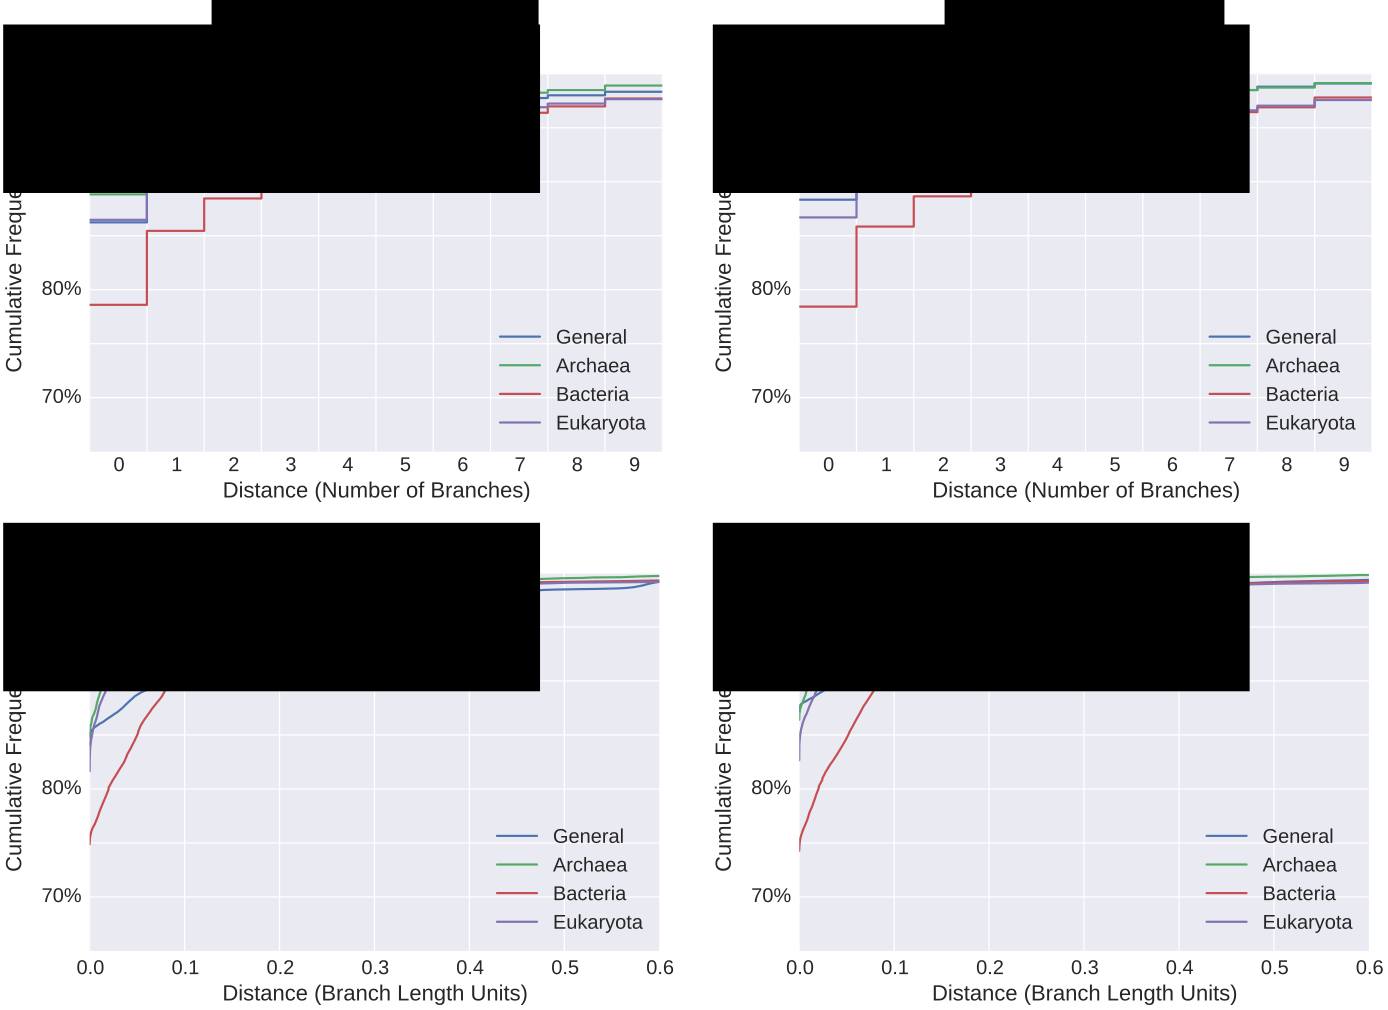
\includegraphics[width=\linewidth]{art/constraints_backbone.pdf}
    \begin{subfigure}{0pt}
        \phantomcaption
        \label{fig:constraints_backbone:sub:edge_unconstr}
    \end{subfigure}
    \begin{subfigure}{0pt}
        \phantomcaption
        \label{fig:constraints_backbone:sub:edge_constr}
    \end{subfigure}
    \begin{subfigure}{0pt}
        \phantomcaption
        \label{fig:constraints_backbone:sub:branch_unconstr}
    \end{subfigure}
    \begin{subfigure}{0pt}
        \phantomcaption
        \label{fig:constraints_backbone:sub:branch_constr}
    \end{subfigure}
    \caption[Accuracy comparison between unconstrained and constrained trees]{
        \textbf{Accuracy comparison between unconstrained and constrained trees.}
        Here, we compare how a taxonomic constraint changes the weighted distances to correct edges
        when placing our evaluation sequences on \acp{PhAT}.
        The evaluation method is explained in the main text.
        Subfigures~\subref{fig:constraints_backbone:sub:edge_unconstr}
        and \subref{fig:constraints_backbone:sub:branch_unconstr} are identical to
        \figref{fig:detail_majorities_backbone} of the main text and included here for ease of comparison.
        Subfigures~\subref{fig:constraints_backbone:sub:edge_constr}
        and \subref{fig:constraints_backbone:sub:branch_constr} show the results when using the
        \toolname{Silva} taxonomy as constraint for the tree inference.
        The relative Robinson-Foulds distances \citep{Robinson1981}
        between the four pairs of trees range between \num{45.8}\% and \num{49.7}\%.
        The differences probably occur because our trees span diverse clades,
        whose ancient branches are hard to resolve. % instead of ``branches'': evolutionary relationships?
        Also, single gene data might not be sufficient to resolve these clades.
        See \secref{sec:DetailsEvaluationReferenceTrees} and \tabref{tab:TreeTopologyTests}
        for a more detailed comparison of the constrained and unconstrained trees.
        However, the differences mostly concern inner branches.
        Most of the placements are however expected to be near the terminal branches,
        which are more stable across the trees.
%         our evaluation process is likely to be not much affected.
        \\
        This is confirmed by the fact that, overall,
        the results are similar between the unconstrained and constrained trees.
        A slight improvement can be observed for the constrained General tree (blue),
        which performs better according to both distance measures.
        However, when considering only the distance of the most likely placement (highest \ac{LWR}) to its correct edge
        instead of using average distances weighted by the \ac{LWR} per \ac{QS},
        the constrained trees consistently yield better results (data not shown).
        For example, the most significant change is observed for the Eukaryota tree,
        with 84\% correct placements for the unconstrained tree, but 89\% for the constrained one.
        We suspect that this is an artifact of our evaluation process,
        as we consider a sequence to be correctly placed if the placement branch belongs to the consensus sequence
        to which the sequence contributed.
        As the selection of sequences for each consensus sequence is guided by the taxonomy,
        using the same taxonomy as constraint for the tree thus might also improve the placement accuracy.
%         Furthermore, the average branch length in all four constrained trees is longer
%         than in their respective unconstrained trees.
%         While this is in accordance with their lower likelihoods (see main text),
%         this further helps in the placement process.
%         furthermore, the constr brings tips closer together, making their dist smaller,
%         in turn making the eval better for seqs that are close to those tips but not exact hits
    }
    \label{fig:constraints_backbone}
\end{figure}

% average branch lengths as mentioned above:
%
% constrained:
%
% arc  0.0717985
% bact 0.0709451
% euk  0.0830736
% gen  0.0859666
%
% avg  0.07794595
% min  0.0709451
% max  0.0859666
%
% unconstrained:
%
% arc  0.0697522
% bact 0.067082
% euk  0.0799271
% gen  0.084141
%
% avg  0.075225575
% min  0.067082
% max  0.084141

% we are not using the continuous histogram plots any more. still, here are some notes that were meant for them:
% things are weighted by the lwr, so half edge dists can exist.
% explain why there are still jumps in the exact plots!
% (because of discrete number of placements per sequence!)
% accumulated percentage of number of placements within a radius of x edges of the correct placement location.
% the distance is weighted by lwrs, that is, the weighted average distance of each pquery is used,
% so that sub-edge resolution of the histogram is possible.

% ======================================================================================================================
%     Consensus Sequences
% ======================================================================================================================

\begin{figure}[hpbt]
    \centering
    \includegraphics[width=\linewidth]{art/consensi_backbone.pdf}
    \begin{subfigure}{0pt}
        \phantomcaption
        \label{fig:consensi_backbone:sub:majorities}
    \end{subfigure}
    \begin{subfigure}{0pt}
        \phantomcaption
        \label{fig:consensi_backbone:sub:cavener}
    \end{subfigure}
    \begin{subfigure}{0pt}
        \phantomcaption
        \label{fig:consensi_backbone:sub:50_threshold}
    \end{subfigure}
%     \begin{subfigure}{0pt}
%         \phantomcaption
%         \label{fig:consensi_backbone:sub:70_threshold}
%     \end{subfigure}
    \begin{subfigure}{0pt}
        \phantomcaption
        \label{fig:consensi_backbone:sub:90_threshold}
    \end{subfigure}
%     \begin{subfigure}{0pt}
%         \phantomcaption
%         \label{fig:consensi_backbone:sub:95_threshold}
%     \end{subfigure}
    \caption[Effect of different consensus sequence methods on placement accuracy]{
        \textbf{Effect of different consensus sequence methods on placement accuracy.}
        In the main evaluation of our \ac{PhAT} method,
        we used a reference tree and alignment based on majority rule consensus sequences \citep{May1952,Day1992a}
        of the \toolname{Silva} database sequences.
        Here, we evaluate the effect of using other consensus sequence methods
        on phylogenetic placement accuracy.
        The evaluation method is described in the main text.
        In addition to \subref{fig:consensi_backbone:sub:majorities} majority rule consensus, we tested
        \subref{fig:consensi_backbone:sub:cavener} Cavener's method \citep{Cavener1987,Cavener1991a},
        as well as threshold consensus sequences \citep{Day1992a,Day1992}
        using thresholds of 50\%, 60\%, 70\%, 80\%, and 90\%, of which two are shown in
        \subref{fig:consensi_backbone:sub:50_threshold} and \subref{fig:consensi_backbone:sub:90_threshold}.
        The three remaining threshold methods exhibit accuracies almost exactly in between the shown plots,
        that is, accuracy decreases with increasing thresholds.
%         and thus are excluded here for simplicity.
        For comparison, we also included \figref{fig:detail_majorities_backbone:sub:num_br} of the main text again,
        here as Subfigure~\subref{fig:consensi_backbone:sub:majorities},
        using the same y-axis scaling as the other plots.
        We only show distances measured in number of branches here,
        because this is more relevant in the context of our methods (e.g., Multilevel Placement).
        % for evaluating phylogenetic placement.
        \\
        By using alternative consensus methods, the consensus sequences and thus the sites in the alignments change.
%         Furthermore, we used random initial starting trees for the tree inference.
        Hence, the obtained reference trees (not shown) differ substantially from each other.
        Across the corresponding trees of the consensus methods tested here,
        we observed an average relative RF distance of 49.5\%.
        This is similar to our findings depicted in in \figref{fig:constraints_backbone}.
        Here too, the accuracy of the constrained variants of these trees (data not shown)
        does not change much compared to the accuracy obtained for the unconstrained trees shown here.
        Thus, the differences in accuracy seen here are most likely due to
        the interplay of alignment and placed sequences (which is what we are interested in),
        and not due to differences in the trees (which are not of interest here).
        \\
        The first three plots \subref{fig:consensi_backbone:sub:majorities}-\subref{fig:consensi_backbone:sub:50_threshold}
        exhibit similar accuracies.
        On average, majority rule, Cavener's, and low threshold ($\leq$ 70\%) consensus methods
        place 82-83\% of the sequences on the expected branch.
        As a general trend, the \taxonname{Archaea}, being the smallest tree, tend to have the highest accuracy.
        On the other hand, the \taxonname{Bacteria}, having the most sequences in \toolname{Silva}, score worst.
        This changes for high consensus thresholds.
        At high thresholds, many sites contain ambiguity characters, thus blurring the phylogenetic signal.
        The \taxonname{General} tree, representing the highest diversity, is most affected by this.
%         as can be seen in the last two plots.
    }
    \label{fig:consensi_backbone}
\end{figure}

% ======================================================================================================================
%     Single Sequences
% ======================================================================================================================

\begin{figure}[hpbt]
    \centering
    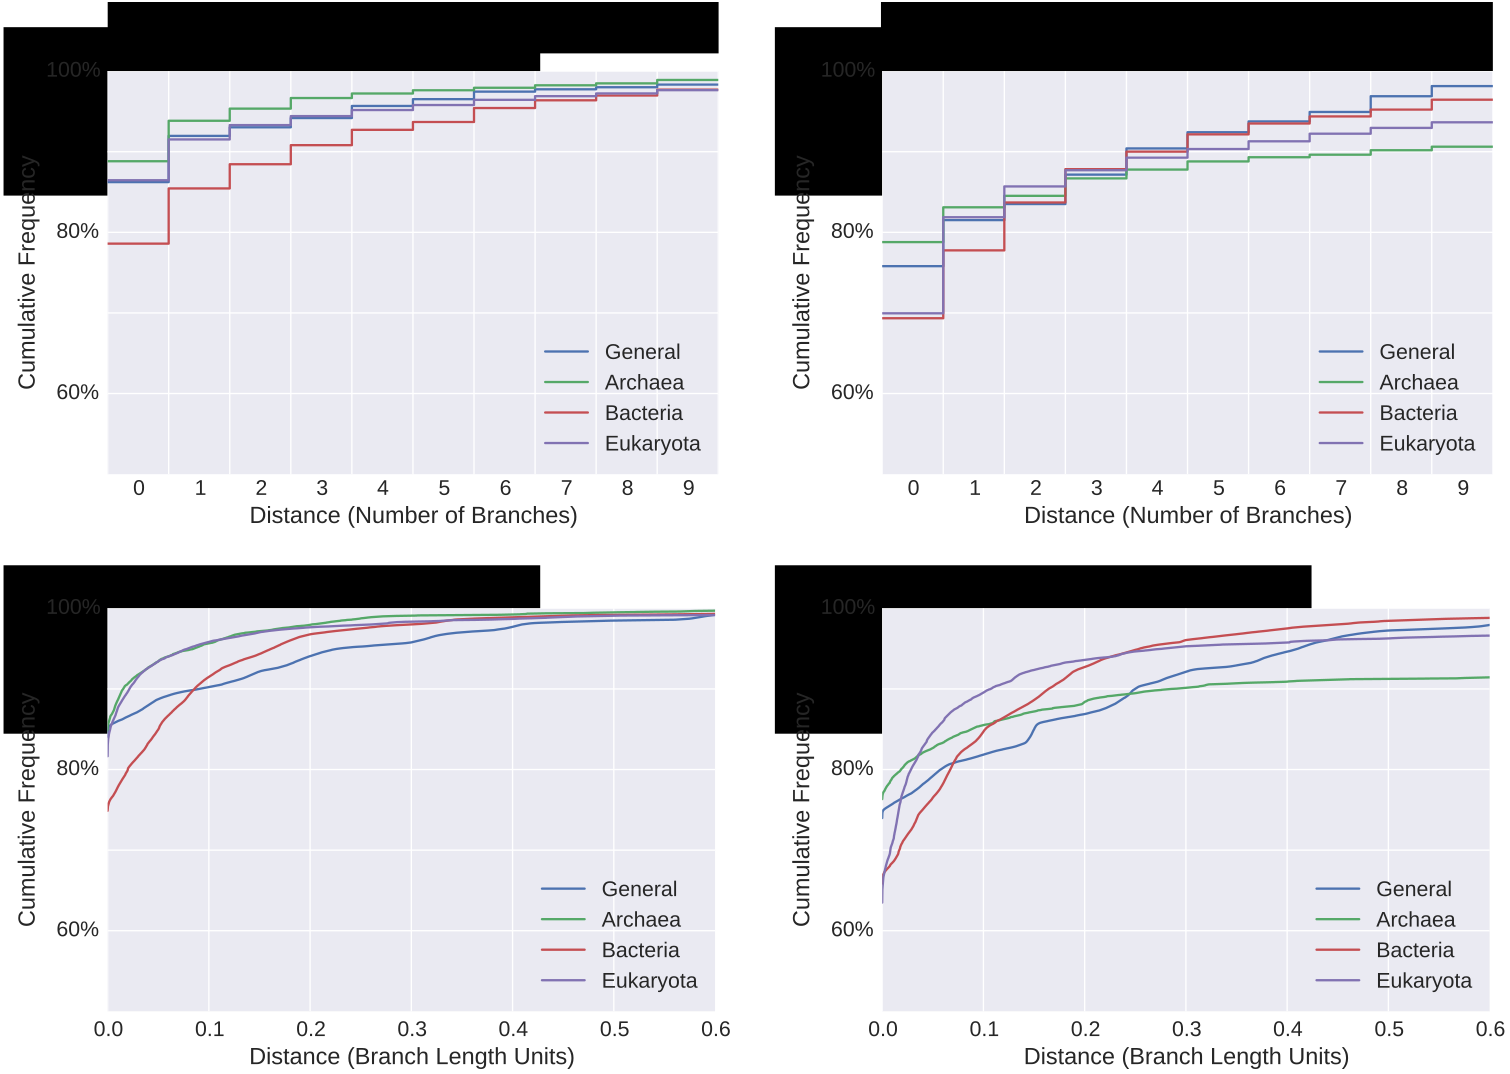
\includegraphics[width=\linewidth]{art/single_seqs.pdf}
    \begin{subfigure}{0pt}
        \phantomcaption
        \label{fig:single_seqs:sub:majorities_edge}
    \end{subfigure}
    \begin{subfigure}{0pt}
        \phantomcaption
        \label{fig:single_seqs:sub:single_seq_edge}
    \end{subfigure}
    \begin{subfigure}{0pt}
        \phantomcaption
        \label{fig:single_seqs:sub:majorities_branch}
    \end{subfigure}
    \begin{subfigure}{0pt}
        \phantomcaption
        \label{fig:single_seqs:sub:single_seq_branch}
    \end{subfigure}
    \caption[Effect of using actual sequences (instead of consensus sequences) on placement accuracy]{
        \textbf{Effect of using actual sequences (instead of consensus sequences) on placement accuracy.}
        For most of our evaluation of the \ac{PhAT} method,
        we used some form of consensus sequence representation for the clades of the taxonomy,
        see e.g., \figref{fig:constraints_backbone} and \figref{fig:consensi_backbone}.
        However, we also tested how the method behaves when using actual sequences instead,
        thus avoiding to unnecessarily blur the phylogenetic signal,
        and other potential drawback of consensus sequences.
        \\
        As manually selecting representative sequences from the database was not practical,
        we used the following automated approach.
        First, we took the 90\% threshold consensus sequences of the \ac{PhAT} method
        that were already evaluated in \figref{fig:consensi_backbone:sub:90_threshold}.
        By using a high threshold, most of the diversity of each clade is included.
        Then, for each such consensus sequence,
        we calculated a score for all sequences from the database that were used to construct this consensus sequence.
        This score is the number of different nucleotides between the consensus sequence and the database sequence.
        The sequence with the lowest score (that is, with most matching nucleotides)
        was then used as representative of the clade.
        Thereby, the taxonomic clades are represented by actual sequences from the database.
        However, as these sequences are close to the respective consensus sequence,
        they are still good representatives of the diversity of the clade.
%         They can hence be considered to be good representatives of the clades.
        Using this set of sequences, we then again inferred a tree and
        conducted the evaluation procedure by placing all sequences of the database on that tree,
        as described in the main text.
        \\
        Subfigures~\subref{fig:single_seqs:sub:majorities_edge}
        and \subref{fig:single_seqs:sub:majorities_branch} are identical to
        \figref{fig:detail_majorities_backbone} of the main text and included here for ease of comparison,
        however with the y-axis scaled to fit the remaining subfigures.
        That is, they show the evaluation of the majority rule consensus sequences.
        Subfigures~\subref{fig:single_seqs:sub:single_seq_edge} and \subref{fig:single_seqs:sub:single_seq_branch}
        show the evaluation of the approach as described here.
        The resulting accuracy is worse in all cases.
        That is, on average, the sequences were placed further from their respective expected branch.
        We suspect that this is because single sequences do not capture the diversity of their clade
        as well as consensus sequences, and because they do not incorporate as much biological information
        (e.g., in form of ambiguity characters).
    }
    \label{fig:single_seqs}
\end{figure}

% ======================================================================================================================
%     Bacteria Tree
% ======================================================================================================================

% \section{Evaluation of Multilevel Placement}
% \label{sec:EvaluationMultilevelPlacement}

\begin{figure}[hpbt]
    \centering
    \includegraphics[width=\linewidth]{art/clades.pdf}
    \caption[Unconstrained \taxonname{Bacteria} tree with five bacterial sub-clades]{
        \textbf{Unconstrained \taxonname{Bacteria} tree with five bacterial sub-clades.}
        This tree is the result of our \ac{PhAT} method
        applied to the \taxonname{Bacteria} sequences in \toolname{Silva}.
        The tree contains a total of 1914 taxa.
        Colorized are the five \taxonname{Phylum} level sub-clades that we used for testing multilevel placement:
        \taxonname{Proteobacteria} (505 taxa), \taxonname{Bacteroidetes} (362 taxa), \taxonname{Firmicutes} (360 taxa),
        \taxonname{Cyanobacteria} (39 taxa) and \taxonname{Actinobacteria} (53 taxa).
        The incongruence between taxonomy and phylogeny is visible here as non-monophyletic colored branches.
        We thus here define a clade to consist of all branches
        that are part of a monophyletic split of the tree with respect to the taxa in the clade.
        In other words, all branches on one side of a split are considered to belong to a clade, %(that is, are colored the same),
        if that side of the split only contains taxa from that clade.
        These branches then receive the same color here.
        Then, for multilevel placement, a sequence is considered to be part of a clade
        if its most probable placement falls into that clade.
        For example, a sequence that is placed onto one of the orange branches on this tree
        is subsequently placed in the \taxonname{Cyanobacteria} tree for the second level placement.
        Each of the five sub-clades is represented by multiple branches here,
        which we call the ``overlap'' with the \taxonname{Bacteria} tree.
    }
    \label{fig:clades}
\end{figure}

% \todo{add a table to the supplement that lists which of our five test clades contains how many seqs in the backbone
% and how many in the second level alignments.}
% \todo{list how many taxa the general tree has for each clade, and how big each clade tree is -- that is, list the number of overlapping taxa.}
% \todo{table of tree sizes? see supp fig}

% ======================================================================================================================
%     BV Comparison
% ======================================================================================================================

\begin{figure}[hpbt]
    \centering
    \includegraphics[width=\linewidth]{art/bv_comparison.pdf}
    \vspace*{-1em}
    \begin{subfigure}{0pt}
        \phantomcaption
        \label{fig:bv_comparison:sub:squash_art}
    \end{subfigure}
    \begin{subfigure}{0pt}
        \phantomcaption
        \label{fig:bv_comparison:sub:squash_orig}
    \end{subfigure}
    \begin{subfigure}{0pt}
        \phantomcaption
        \label{fig:bv_comparison:sub:edgepca_art}
    \end{subfigure}
    \begin{subfigure}{0pt}
        \phantomcaption
        \label{fig:bv_comparison:sub:edgepca_orig}
    \end{subfigure}
    \caption[Assessment of a \ac{PhAT} for conducting Squash Clustering and Edge PCA]{
        \small
        \todo{this is small. lets see if this needs to stay small!}
        \textbf{Assessment of a \ac{PhAT} for conducting Squash Clustering and Edge PCA.}
        Here, we test the behavior of the unconstrained \taxonname{Bacteria} tree obtained via our \ac{PhAT} method
        when used for standard post-analyses of phylogenetic placement results.
        For this, we used a sequence dataset of the vaginal microbiome of 220 women \citep{Srinivasan2012}.
        For details on the processing, see \secref{ch:EmpiricalDatasets}.
%         containing a total of \num{426 612} sequences.
        The original study showed associations between the presence of certain bacterial species
        and the diagnosis of \acf{BV}, a condition caused by changes in the vaginal microbiome.
        In the study, the Nugent score \citep{Nugent1991} was used as a clinical diagnostic criterion for \ac{BV},
        which ranges from \num{0} (healthy) to \num{10} (severe illness).
        We placed the sequences of the dataset on their original tree and on our \ac{PhAT},
        and reproduce some of the results from the original study
%         by performing Squash Clustering and Edge PCA on the data
        to assess differences induced by using distinct references trees.
%         Each colored dot in the figure represents one sample.
        \\
        Squash Clustering is a hierarchical clustering method for phylogenetic placement data \citep{Matsen2011a} % and Srinivasan2012
%         It is a generalization of the UniFrac distance \citep{Lozupone2005,Lozupone2007a},
%         and yields meaningful branch lengths of the cluster tree.
%         To this end, it
        that uses the phylogenetic Kantorovich-Rubinstein (KR) distance \citep{Evans2012} % and Matsen2011a
%         also known as the Wasserstein distance, Mallows distance,
%         or Earth Mover's distance \citep{Mallows1972,Rachev1985,Levina2001,Villani2008},
        to measure cluster similarity.
        The result of Squash Clustering is a cluster tree of samples,
        where samples that are similar according to the KR distance are closer to each other,
        with branch lengths according to that distance.
        The left side of the figure compares the cluster trees resulting from using
        \subref{fig:bv_comparison:sub:squash_art}  our tree and
        \subref{fig:bv_comparison:sub:squash_orig} the original reference tree.
        Subfigure \subref{fig:bv_comparison:sub:squash_orig} is a recalculation of Figure~1(A) of \citep{Srinivasan2012}.
        The tips, which correspond to samples, are colored by the Nugent score of each sample,
        and thus indicate which women are affected by \ac{BV}.
        The general features of the two cluster trees are comparable,
        indicating that our tree is able to distinguish between healthy and sick patients.
        However, there is a major difference in the lower half of the trees:
        While \subref{fig:bv_comparison:sub:squash_orig} shows some small branch lengths and even a separated sub-clade
        of samples with low Nugent score,
        these branches have a length of virtually zero in \subref{fig:bv_comparison:sub:squash_art}.
        As shown in \citep{Srinivasan2012}, the healthy patients are divided into two classes,
        based on the presence of two species of \taxonname{Lactobacillus}.
        The original reference tree contains sequences of those species, and can thus distinguish between them.
        Our broad \taxonname{Bacteria} tree however
        does not have this degree of species-level resolution and thus treats them the same,
        yielding a negligible KR distance between the samples.
        Although this finding is expected, it serves as an example for the limits of our method.
        \todo{missing text!!!!!!!!!!!!!!!!!!!!!!!!!!!!!!!!!!!!!!!!!!!!!!! dimensions too large!}
%         \\
%         This can also be seen in the right side of the figure, where we compare Edge PCA using
%         \subref{fig:bv_comparison:sub:edgepca_art} our \ac{PhAT} and
%         \subref{fig:bv_comparison:sub:edgepca_orig} the original reference tree.
%         Edge PCA \citep{Matsen2011a} is a dimensionality reduction method for phylogenetic placement data,
%         which can visualize differences between samples.
%         Subfigure \subref{fig:bv_comparison:sub:edgepca_orig} is a recalculation of Figure~3(A) of \citep{Srinivasan2012}.
%         While our tree is able to separate samples by Nugent score,
%         it does not exhibit the further separation of the two \taxonname{Lactobacillus} species
%         that is apparent when using the original tree.
%         Thus, the samples with low Nugent score form one blob in \subref{fig:bv_comparison:sub:edgepca_art}.
%         \\
%         This limitation can be overcome by either resolving the \ac{PhAT} down to species level,
%         or by using multilevel placement with a refined tree
%         that for example contains species sequences of the relevant \taxonname{Lactobacillus} clades.
%         We however generally note that similar issues of deficient resolution or missing species
%         can potentially also arise when hand-selecting reference sequences.
%         In the end, it is the responsibility of the researcher to make sure that the selection of reference sequences
%         is suitable for the dataset to be placed.
    }
    \label{fig:bv_comparison}
\end{figure}

% ======================================================================================================================
%     HMP Comparison
% ======================================================================================================================

\begin{figure}[hpbt]
    \centering
    \includegraphics[width=\linewidth]{art/mds_epca.pdf}
    \begin{subfigure}{0pt}
        \phantomcaption
        \label{fig:hmp_mds_epca:sub:mds}
    \end{subfigure}
    \begin{subfigure}{0pt}
        \phantomcaption
        \label{fig:hmp_mds_epca:sub:edge_pca}
    \end{subfigure}
    \caption[Assessment of a \ac{PhAT} for large dataset analyses]{
        \textbf{Assessment of a \ac{PhAT} for large dataset analyses.}
        Here, we test the unconstrained \taxonname{Bacteria} tree generated by our \ac{PhAT} method
        for placing and analyzing a large sequence dataset.
        For this, we use the Human Microbiome Project (HMP) \citep{Huttenhower2012,Methe2012} data,
        and selected \num{9192} samples from different body sites with a total of 117 million sequences.
        For details on the processing, see \secref{ch:EmpiricalDatasets}.
        We categorized the 19 original body site labels into 8 regions, in order to make the plot more readable.
        See \tabref{tab:hmp_data_overview} for the mapping between the original labels and the ones used here.
        The sequences were placed on the tree, and subsequently analyzed with two different methods.
        Both subfigures show that the tree, despite only representing higher taxonomic levels,
        suffices to separate different body site regions from each other.
%         Even different oral regions are mostly separated, although there seems to be quite some overlap.
        \\
        In subfigure \subref{fig:hmp_mds_epca:sub:mds}, we visualized the pairwise KR distances between all samples.
        The phylogenetic Kantorovich-Rubinstein (KR) distance \citep{Matsen2011a,Evans2012} between two samples,
        also known as the Earth Mover's distance,
        measures how much placement ``mass'' has to be moved by how much along the branches of the tree
        in order to transform one sample into the other.
        It is a generalization of the UniFrac distance \citep{Lozupone2005,Lozupone2007a}.
        The high-dimensional pairwise KR distance matrix was then embedded into the plot by performing \acf{MDS}.
        \ac{MDS} \citep{Mardia1978,Krzanowski1994,Everitt2010} is a dimensionality reduction technique that
        finds an embedding of a distance matrix into lower dimensions (in this case, \num{2} dimensions)
        preserving higher dimensional distances as well as possible.
        \\
        In subfigure \subref{fig:hmp_mds_epca:sub:edge_pca}, we also perform Edge PCA \citep{Matsen2011a}
        on the samples.
        The grouping of body sites is again clearly visible with this method.
%         See \figref{fig:bv_comparison} for a short explanation of this method.
        Similar to \figref{fig:bv_comparison:sub:edgepca_orig}, the plot forms a triangle of samples,
        roughly separated by body site regions.
    }
    \label{fig:hmp_mds_epca}
\end{figure}

% ======================================================================================================================
%     Multilevel Placement
% ======================================================================================================================

\begin{figure}[hpbt]
    \centering
    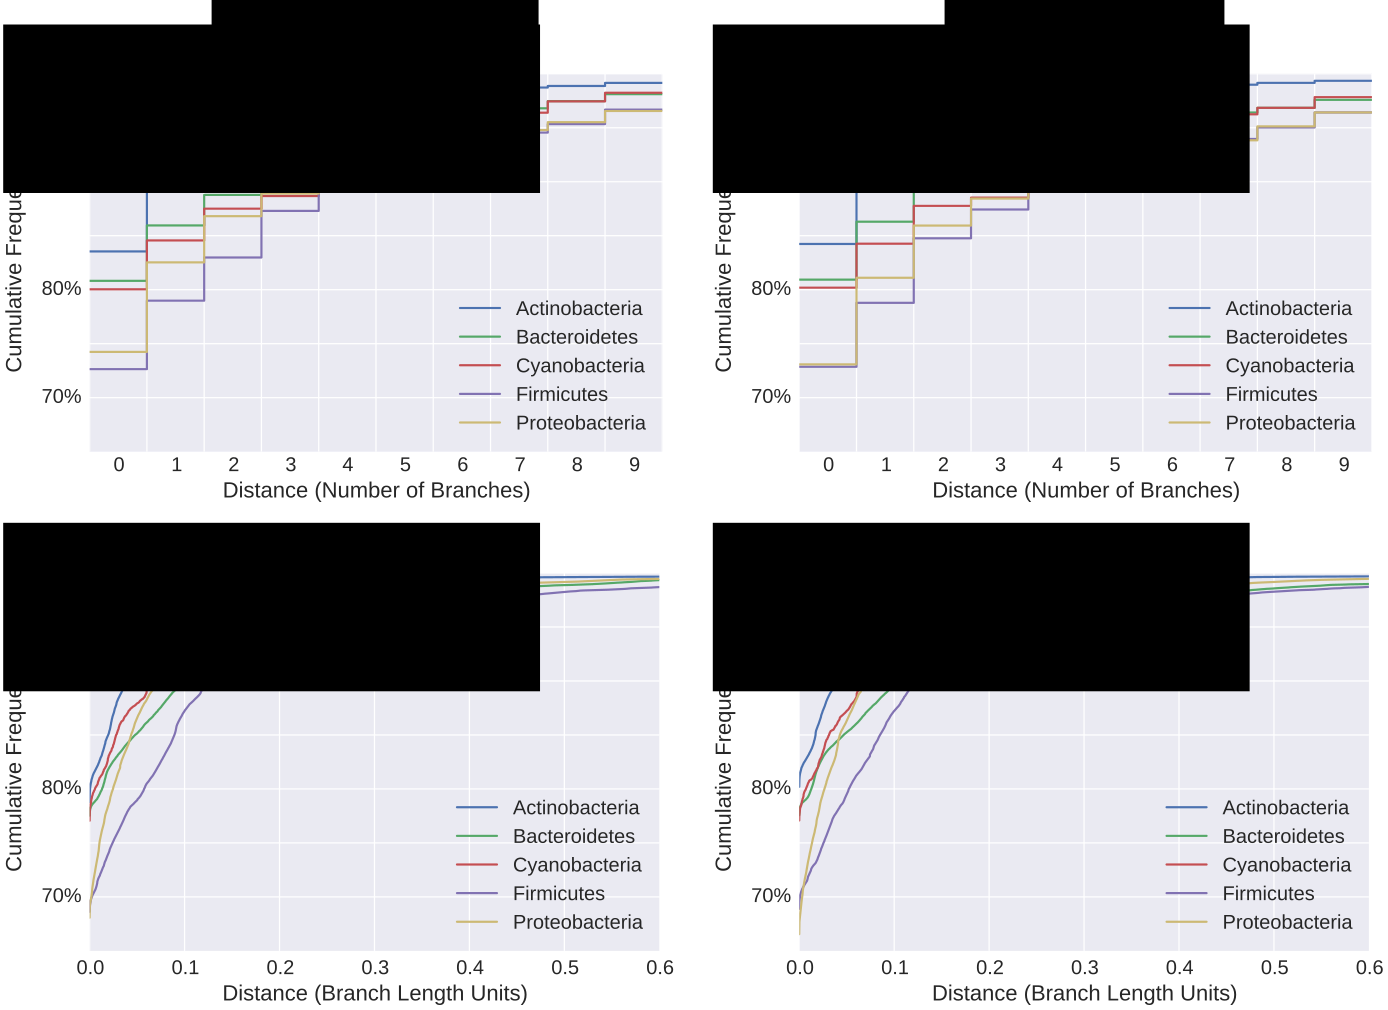
\includegraphics[width=\linewidth]{art/multilevel.pdf}
    \begin{subfigure}{0pt}
        \phantomcaption
        \label{fig:multilevel:sub:edge_unconstr}
    \end{subfigure}
    \begin{subfigure}{0pt}
        \phantomcaption
        \label{fig:multilevel:sub:edge_constr}
    \end{subfigure}
    \begin{subfigure}{0pt}
        \phantomcaption
        \label{fig:multilevel:sub:branch_unconstr}
    \end{subfigure}
    \begin{subfigure}{0pt}
        \phantomcaption
        \label{fig:multilevel:sub:branch_constr}
    \end{subfigure}
    \caption[Accuracy of the \acp{PhAT} of five bacterial sub-clades]{
        \textbf{Accuracy of the \acp{PhAT} of five bacterial sub-clades.}
        We used five sub-clades of the \taxonname{Bacteria} in \toolname{Silva},
        which were already scrutinized in \citep{Kozlov2016},
        to test how our \ac{PhAT} method works for less diverse sets of sequences.
        These five clades are also highlighted in \figref{fig:clades};
        see there for a description of the clades.
        The evaluation was conducted as explained in the main text;
        in short, we placed the \toolname{Silva} sequences of the clades on their respective tree,
        and measured how far each of them is away from the branch of the consensus sequence it is represented by.
%         The figure follows \figref{fig:constraints_backbone} in layout.
        \\
        The placement accuracy on these sub-clades is slightly worse compared to the broad \taxonname{Bacteria} tree,
        which can be seen by comparison to \figref{fig:constraints_backbone}.
        On average, 73.4\% of the sequences were placed exactly on their expected branch,
        dominated by \taxonname{Proteobacteria} and \taxonname{Firmicutes},
        which combined make up 75\% of the sequences in the five clades, and have an accuracy of 71\%.
        The \taxonname{Actinobacteria} have the highest accuracy,
        with 82\% of their sequences placed on the expected branch.
        \\
%         There are however also differences between the clades.
        The two smallest clades, \taxonname{Actinobacteria} and \taxonname{Cyanobacteria},
        exhibit the shortest distances in branch length units.
        In fact, the longest distance of any sequence from its expected branch in the \taxonname{Cyanobacteria} clade
        is around \num{0.4}, which is indicated by the end of the red line in the lower two plots.
        On the other hand, the \taxonname{Firmicutes} generally have the lowest accuracy here.
        In \figref{fig:clades}, which shows the unconstrained \taxonname{Bacteria} tree,
        the \taxonname{Firmicutes} clade exhibits many paraphyletic branches,
        which is a known issue \citep{Parks2018}.
        This indicates that there is a high incongruence
        between the \taxonname{Firmicutes} taxonomy and phylogeny in \toolname{Silva},
        which might explain why the \taxonname{Firmicutes} score worst here.
        \\
        These results are likely due to the inability of 16S SSU sequences to properly resolve lower taxonomic levels
        \citep{Mignard2006,Petti2007,Janda2007}.
        For example, Table 2 of \citep{Janda2007} lists \num{10} bacterial genera
        that are known to be hard to identify using 16S sequences.
        These genera account for \num{7.9}\% of the \num{2846} taxa
        that are represented by the five bacterial trees tested here.
        Furthermore, \num{95 553} of the \num{450 313} sequences that were placed on those trees (\num{21.2}\%)
        belong to one of these genera.
        This might explain the worse scores of these clade trees.
        Lastly, the consensus sequences at the tips of the trees represent the \taxonname{Genus} level.
        Thus, these have short branches, which increases the probability of misplacements.
%         the Cyanobacteria (red) ends, because there are no more placements further away from their correct edges than this.
%         this shows short branches etc. get avg branch lenghts of those trees!
%         number of taxa, number of sequences for each tree!
%
%         and to give an example of how multilevel placement works.
%         we do not trust species level placement anyway. see main text
    }
    \label{fig:multilevel}
\end{figure}

% from top eval in /home/lucas/Projects/bacardi/02\_multilevel/05\_accuracy\_viz
% Actinobacteria  Correct pqueries 0: 41590 / 50700 = 0.820316
% Cyanobacteria   Correct pqueries 0: 8901 / 11180 = 0.796154
% Proteobacteria  Correct pqueries 0: 138944 / 195517 = 0.710649
% Firmicutes      Correct pqueries 0: 98417 / 138460 = 0.710797
% Bacteroidetes   Correct pqueries 0: 38924 / 49144 = 0.79204
% total                               326776      445001      0.7343264397

% for mean genera listing, see  02_multilevel/06_mean_genera

% Subtree Phyla
% ==========================
%
% Cyanobacteria
% 94 taxa
% 11,379 sequences
%
% Proteobacteria
% 1,569 taxa
% 200,083 sequences
%
% Firmicutes
% 652 taxa
% 138,636 sequences
%
% Bacteroidetes
% 440 taxa
% 49,214 sequences
%
% Actinobacteria
% 494 taxa
% 51,160 sequence

% ======================================================================================================================
%     CAMI Performance
% ======================================================================================================================

\begin{figure*}[hpbt]
    \centering
    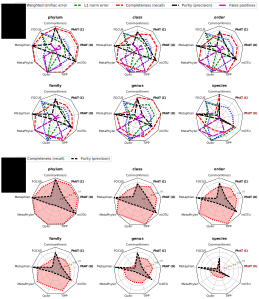
\includegraphics[width=0.94\linewidth]{art/cami_performance.pdf}
    \begin{subfigure}{0pt}
        \phantomcaption
        \label{fig:cami_performance:sub:relative}
    \end{subfigure}
    \begin{subfigure}{0pt}
        \phantomcaption
        \label{fig:cami_performance:sub:absolute}
    \end{subfigure}
    \caption[CAMI: Profiling Results]{
        \textbf{CAMI: Profiling Results.}
        The figure shows the profiling results of different tools evaluated with data from, and following the protocol of,
        the 2nd CAMI challenge \citep{Sczyrba2017,Bremges2018}.
        Here, we compare the taxonomic assignment and profiling conducted with our \texttt{assign} command
        to the tools that took part in the 2nd CAMI challenge.
        For this, we used the unconstrained and constrained \taxonname{Bacterial} tree,
        which are abbreviated here as ``PhAT (U)'' and ``PhAT (C)'', respectively.
        See \secref{sec:Results:sub:TaxonomicAssignmentProfilingDetails} for details on our evaluation,
        and see \cite{Sczyrba2017} for details on CAMI and their metrics.
        \\
        Subfigure \subref{fig:cami_performance:sub:relative} shows the relative performance of the tools
        for different taxonomic ranks by displaying the error metrics used by CAMI:
        Weighted Unifrac error, L1 norm error, recall (completeness), precision (purity) and false positives.
        The error metrics were divided by their respective maximal value to allow viewing them on the same scale
        and to allow relative performance comparisons.
%         \\
        Subfigure \subref{fig:cami_performance:sub:absolute} shows the absolute recall (completeness) and precision (purity)
        for each tool across the taxonomic ranks.
%         \\
        In both subfigures, the red text for our PhAT evaluations indicates
        that no predictions at the corresponding taxonomic rank were returned.
        This is because our \toolname{Silva}-based tree does not have \taxonname{species} resolution
        and does hence not allow for taxonomic profiling at this level.
    }
    \label{fig:cami_performance}
\end{figure*}

% % ======================================================================================================================
% %     CAMI Relative Performance
% % ======================================================================================================================
%
% \begin{figure*}[hpbt]
%     \centering
%     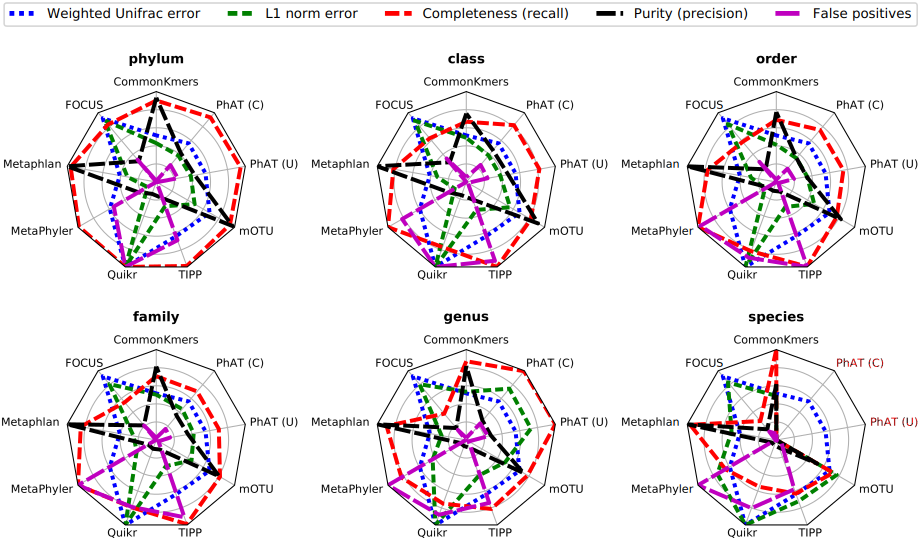
\includegraphics[width=\linewidth]{img/spider_plot.pdf}
%     \vspace{1em}
%     \caption{
%         \textbf{CAMI: Relative Performance.}
%         bla bla
%     }
%     \label{fig:spider_plot}
% \end{figure*}
%
% % ======================================================================================================================
% %     CAMI Absolute Performance
% % ======================================================================================================================
%
% \begin{figure*}[hpbt]
%     \centering
%     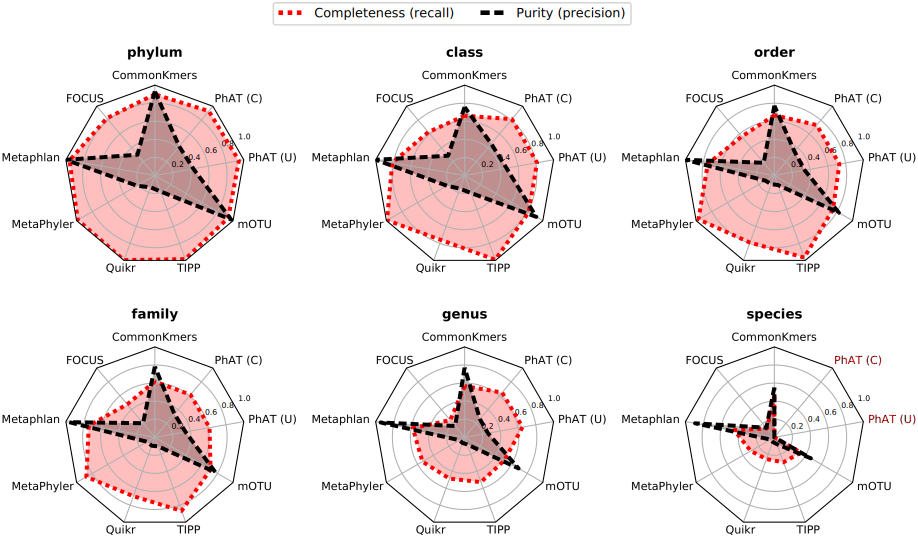
\includegraphics[width=\linewidth]{img/spider_plot_recall_precision.pdf}
%     \vspace{1em}
%     \caption{
%         \textbf{CAMI: Absolute Performance.}
%         bla bla
%     }
%     \label{fig:spider_plot_recall_precision}
% \end{figure*}

% ======================================================================================================================
%     CAMI Alpha Diversity
% ======================================================================================================================

\begin{figure}[hpbt]
    \centering
    \includegraphics[width=\linewidth]{art/alpha_diversity.pdf}
    \begin{subfigure}{0pt}
        \phantomcaption
        \label{fig:alpha_diversity:sub:total}
    \end{subfigure}
    \begin{subfigure}{0pt}
        \phantomcaption
        \label{fig:alpha_diversity:sub:difference}
    \end{subfigure}
    \caption[CAMI: Alpha Diversity]{
        \textbf{CAMI: Alpha Diversity.}
        The figure shows the alpha diversity as estimated by different tools evaluated
        with data from, and following the protocol of, the 2nd CAMI challenge \citep{Sczyrba2017,Bremges2018}.
        Here, we compare the taxonomic assignment and profiling conducted with our \texttt{assign} command
        to the tools that took part in the 2nd CAMI challenge.
        For this, we used the unconstrained and constrained \taxonname{Bacterial} tree,
        which are abbreviated here as ``PhAT (U)'' and ``PhAT (C)'', respectively.
%         See Supplementary Section~\ref{sec:TaxonomicAssignment} for details.
%         \\
        \todo{add some more text here}
    }
    \label{fig:alpha_diversity}
\end{figure}

% ######################################################################################################################
%         Visualization
% ######################################################################################################################

\chapter{Visualization}
\label{ch:Visualization}

\paperbox{
    This chapter is based on the peer-reviewed publication:
}{\paperpppp}{
    \textbf{Contributions:} Lucas Czech... Alexandros Stamatakis...
}

% ######################################################################################################################
%         Motivation
% ######################################################################################################################

\section{Motivation}
\label{ch:Visualization:sec:Motivation}

A first step in analyzing phylogenetic placement data is often to visualize them.
For small samples, it is possible to mark individual placement locations on the \ac{RT},
as offered for example by \toolname{iTOL} \cite{Letunic2016},
or even to create a tree where the most probable placement per \ac{QS} is attached as a new branch,
as implemented in the \toolname{guppy} tool from the \toolname{pplacer} suite \cite{Matsen2010},
\toolname{RAxML-EPA} \cite{Berger2011,Stamatakis2014}, and our tool \toolname{gappa}.
For larger samples, one can alternatively display the per-edge placement mass,
either by adjusting the line widths of the edges according to their mass, or by using a color scale,
as offered in \toolname{ggtree} \cite{Yu2017}, \toolname{guppy}, and \toolname{gappa}.
Using per-edge colors corresponds to binning all placement of an edge into one bin.
%it is thinkable to use multiple bins instead, too, resulting in edges split into segments with different colors.
For large datasets, the per-edge masses can vary by several orders of magnitude.
In these cases, it is often preferable to use a logarithmic scaling, as shown in \cite{Mahe2017}.
%In addition to visualizing each sample separately, the average mass distribution gives an overview of a set of samples.

These simple visualizations directly depict the placement masses on the tree.
When visualizing the accumulated masses of multiple samples at once,
it is important to chose the appropriate normalization strategy for the task at hand.
For example, if samples represent different locations, one might prefer to use normalized masses,
as comparing relative abundances is common for this type of data.
On the other hand, if samples from the same location are combined
(e.g., from different points in time, or different size fractions),
it might be preferable to use absolute abundances instead,
so that the total number of sequences per sample can be visualized.

The visualizations provide an overview of the species abundances over the tree.
They can be regarded as a more detailed version of classic abundance pie charts.
When placing OTUs, or ignoring sequence abundances, the resulting visualizations depict species diversity.
% Those two figures can even be combined into one by adding brackets with abundances
% around the clades of the tree when drawing it.
% When drawing the tree, abundances can also be annotated around its clades,
% effectively combining those two figures into one.
Moreover, these visualizations can be used to assess the quality of the \ac{RT}.
% No ``zone'' here? Micah will be disappointed...
% The inner edges of the \ac{RT} form a zone of older evolutionary relationships.
% Placements into that zone may indicate that appropriate reference sequences
For example, placements into inner branches of the \ac{RT} may indicate that appropriate reference sequences
(i) have not been included or (ii) are simply not yet available.
%This complements the sequence filtering that relies on so-called backbone trees
% as described in \nameref{sec:Preprocessing::sub:MultilevelPlacement}.
%that we recently introduced \cite{Czech2018}.

Here, we introduce visualization methods that highlight
(i) regions of the tree with a high variance in their placement distribution (called \emph{Edge Dispersion}),
and (ii) regions with a high correlation to meta-data features (called \emph{Edge Correlation}).

% ######################################################################################################################
%         Edge Dispersion
% ######################################################################################################################

\section{Edge Dispersion}
\label{ch:Visualization:sec:EdgeDispersion}

The Edge Dispersion is derived from the edge masses or edge imbalances matrix by
calculating a measure of dispersion for each of the matrix columns, for example the standard deviation $\sigma$.
Because each column corresponds to an edge, this information can be mapped back to the tree,
and visualized, for instance, via color coding.
% Edges with a high variance indicate parts of the tree with...
This allows to examine which edges exhibit a high heterogeneity of placement masses across samples,
% vary in terms of their placements,
and indicates which edges discriminate samples.
As edge mass values can span many orders of magnitude,
it might be necessary to scale the variance logarithmically. %, % as shown in Figure~\ref{fig:var_cor:sub:em_varl},
%or to use some other form of normalization.
Often, one is more interested in the branches with high placement mass.
In these cases, using the standard deviation or variance is appropriate,
as they also indicate the mean mass per edge.
On the other hand, by calculating the per-edge Index of Dispersion \cite{Everitt2010},
that is, the variance-mean-ratio $\sfrac{\sigma^2}{\mu}$,
differences on edges with little mass also become visible.
As Edge Dispersion relates placement masses from different samples to each other,
the choice of the normalization strategy {\em is} important.
When using normalized masses, the magnitude of dispersion values needs to be cautiously interpreted \cite{Lovell2015}.
% \todo{maybe we should mention here that this is valid because masses are a zero-based dimension?!}
% \todo{furthermore, Index of Dispersion is often used to compare to a Poisson distribution,
% which we however do not expect from masses. maybe this is still interesting}
The Edge Dispersion can also be calculated for edge imbalances.
As edge imbalances are usually normalized to $[ -1.0, 1.0 ]$,
their dispersion can be visualized directly without any further normalization steps.
% Because imbalances can be negative, the Index of Dispersion is not applicable to them.
An example for an Edge Dispersion visualization is shown in \figref{fig:var_cor:sub:em_varl},
and discussed in Section \nameref{ch:Visualization:sec:Results}.

\begin{figure}[!ht]
    \centering
%     \includegraphics[width=\linewidth]{img/var_cor.pdf}
    \begin{subfigure}{0pt}
        \phantomcaption
        \label{fig:var_cor:sub:em_varl}
    \end{subfigure}
    \begin{subfigure}{0pt}
        \phantomcaption
        \label{fig:var_cor:sub:ei_var}
    \end{subfigure}
    \caption[Examples of Edge Dispersion and Edge Correlation]{
        \textbf{Examples of Edge Dispersion and Edge Correlation.}
        We applied our novel visualization methods to the \ac{BV} dataset
        to compare them to the existing examinations of the data.
%         See \cite{Srinivasan2012} for details of the dataset and its interpretation.
        \subref{fig:var_cor:sub:em_varl}
        Edge Dispersion, measured as the standard deviation of the edge masses across samples, logarithmically scaled.
        \subref{fig:var_cor:sub:ei_var}
        Edge Correlation, in form of Spearman's Rank Correlation Coefficient
        between the edge imbalances and the Nugent score.
        Tip edges are gray, because they do not have a meaningful imbalance.
        This example also shows the characteristics of edge masses and edge imbalances:
        The former highlights individual edges, the latter paths to clades.
%         Note that in this case, both methods highlight similar parts of the tree.
    }
    \label{fig:var_cor}
\end{figure}

% ######################################################################################################################
%         Edge Correlation
% ######################################################################################################################

\section{Edge Correlation}
\label{ch:Visualization:sec:EdgeCorrelation}

In addition to the per-edge masses, the Edge Correlation further
takes a specific meta-data feature into account, that is, a column of the meta-data matrix.
The Edge Correlation is calculated as the correlation between each edge column and the feature column,
for example by using the Pearson Correlation Coefficient or Spearman's Rank Correlation Coefficient \cite{Everitt2010}.
This yields a per-edge correlation of the placement masses or imbalances with the meta-data feature,
and can again be visualized via color coding of the edges.
It is inexpensive to calculate and hence scales well to large datasets.
As typical correlation coefficients are within $[ -1.0, 1.0 ]$, there is again no need for further normalization.
This yields a tree where edges or clades with either a high linear or monotonic correlation
with the selected meta-data feature are highlighted.
\figref{fig:var_cor:sub:ei_var} shows an example of this method.
In contrast to Edge PCA \cite{Matsen2011a} that can use meta-data features to annotate samples in its scatter plots,
our Edge Correlation method directly represents the influence of a feature on the branches or clades of the tree.
It can thus, for example, help to identify and visualize dependencies
between species abundances and environmental factors such as temperature or nutrient levels.
Again, the choice of normalization strategy is important to draw meaningful conclusions.
However, the correlation is \emph{not} calculated between samples or sequence abundances.
% the masses are not put into correlation with each other
Hence, even when using normalized samples, %that is, working with compositional data,
the pitfalls regarding correlations of compositional data \cite{Lovell2015} do not apply here.

% correlation: not correlating masses to each other, so the caveat does not apply.
% not setting compositional values in correlation with each other, so the pitfall schnappt nicht zu
% we simply say: relatively more on that branch, if higher metadata value

% ######################################################################################################################
%         Results
% ######################################################################################################################

\section{Results}
\label{ch:Visualization:sec:Results}

% ----------------------------------------------------------------------------------------------------------------------
%     BV Dataset
% ----------------------------------------------------------------------------------------------------------------------

\subsection{BV Dataset}
\label{ch:Visualization:sec:Results:sub:BVDataset}

We re-analyzed the \ac{BV} dataset by inferring a tree from the original reference sequence set
and conducting phylogenetic placement of the \num{220} samples.
The characteristics of this dataset were already explored in \cite{Srinivasan2012} and \cite{Matsen2011a}.
We use it here to give exemplary interpretations of our Edge Dispersion and Edge Correlation methods,
and to evaluate them in comparison to existing methods.

\figref{fig:var_cor} shows our novel visualizations of the \ac{BV} dataset.
Edge Dispersion is shown in \figref{fig:var_cor:sub:em_varl},
% using the standard deviation of the edge masses, logarithmically scaled.
while \figref{fig:var_cor:sub:ei_var} shows Edge Correlation with the so-called Nugent score. % with the edge imbalances.
The Nugent score \cite{Nugent1991} is a clinical standard for the diagnosis of Bacterial Vaginosis,
ranging from \num{0} (healthy) to \num{10} (severe illness).
The connection between the Nugent score and the abundance of placements on particular edges
was already explored in \cite{Matsen2011a}, but only visualized indirectly (i.e., not on the \ac{RT} itself).
For example, Figure~6 of the original study plots the first two Edge PCA components colorized by the Nugent score.
We recalculated this figure for comparison in \figref{fig:kmeans_all:sub:epca_ns}.
In contrast, our Edge Correlation measure directly reveals the connection between Nugent score and placements on the reference tree:
The clade on the left hand side of the tree, to which the red and orange branches lead to,
are \taxonname{Lactobacillus iners} and \taxonname{Lactobacillus crispatus}, respectively,
which were identified in \cite{Srinivasan2012} to be associated with a healthy vaginal microbiome.
Thus, their presence in a sample is anti-correlated with the Nugent score, which is lower for healthy subjects.
The branches leading to this clade are hence colored in red.
On the other hand, there are several other clades that exhibit a positive correlation with the Nugent score,
that is, were green and blue paths lead to in the figure,
again a finding already reported in \cite{Srinivasan2012}.

Both trees in \figref{fig:var_cor} highlight the same parts of the tree:
The dark branches with high deviation in \figref{fig:var_cor:sub:em_varl} represent clades
attached to either highly correlated (blue) or anti-correlated (red) paths \figref{fig:var_cor:sub:ei_var}.
This indicates that edges that have a high dispersion
also vary between samples of different Nugent score.
% This indicates that both methods reveal the clades that are relevant for discriminating samples of this dataset.

We further compared our methods to the visualization of Edge PCA components on the reference tree.
To this end, we recalculated Figures 4 and 5 of \cite{Matsen2011a},
and visualized them with our color scheme in \figref{fig:epca} for ease of comparison.
They show the first two components of Edge PCA, mapped back to the \ac{RT}.
The first component %, \figref{fig:epca:sub:comp1},
reveals that the \taxonname{Lactobacillus} clade represents the axis with the highest heterogeneity across samples,
while the second component%, \figref{fig:epca:sub:comp2},
further distinguishes between the two aforementioned clades within \taxonname{Lactobacillus}.
Edge Correlation also highlights the \taxonname{Lactobacillus} clade as shown in \figref{fig:var_cor:sub:ei_var},
but does not distinguish further between its sub-clades.
This is because a high Nugent score is associated
with a high abundance of placements in either of the two relevant \taxonname{Lactobacillus} clades.
% In other words, Edge Correlation only reveals information that is associated with the used meta-data feature.

Further examples of variants of Edge Dispersion and Edge Correlation on this dataset
are shown in \figref{fig:all_dispersions} and \figref{fig:all_nugent}.
We also conducted Edge Correlation using Amsel's criteria \cite{Amsel1983} and the vaginal pH value as shown in \figref{fig:amsel_ph},
both of which were used in \cite{Srinivasan2012} as additional indicators of Bacterial Vaginosis.
We again found similar correlations compared to the Nugent score.

% ----------------------------------------------------------------------------------------------------------------------
%     Tara Dataset
% ----------------------------------------------------------------------------------------------------------------------

\subsection{Tara Oceans Dataset}
\label{ch:Visualization:sec:Results:sub:TaraDataset}

We analyzed the \ac{TO} dataset to provide further exemplary use cases for our visualization methods.
To this end, we used the unconstrained \taxonname{Eukaryota} \ac{RT} with \num{2059} taxa
as provided by our Automatic Reference Tree method \cite{Czech2018}.
The meta-data features of this dataset that best lend themselves to our methods are the sensor values for
chlorophyll, nitrate, and oxygen concentration, as well as the salinity and temperature of the water samples.
Other available meta-data features such as longitude and latitude are available,
but would require more involved methods.
This is because geographical coordinates yield pairwise distances between samples,
whose integration into our correlation analysis methods is challenging.
The Edge Correlation of the \num{370} samples with the nitrate concentration, the salinity, the chlorophyll concentration,
and the water temperature are shown in \figref{fig:tara_correlation}.

We selected the diatoms and the animals as two exemplary clades for closer examination of the results.
In particular, the diatoms show a high correlation with the nitrate concentration,
as well as an anti-correlation with salinity, which represent well-known relationships \cite{Lozupone2007,Potapova2011}.
See \figref{fig:tara_correlation} for details.
These findings indicate that the method is able to identify known relationships.
It will therefore also be useful to investigate or discover
insights of novel relationships between sequence abundances and environmental parameters.

% In both cases, the \taxonname{Diatoms} exhibit the most obvious correlation with those meta-data features.
% Diatoms are mainly photosynthetic, and thus rely on nitrogen,
% which explains the high correlating of their clade as shown in \figref{fig:tara_correlation:sub:nitrate}.
% On the other hand, they prefer environments with low salt concentrations,
% which is indicated by the anti-correlation in \figref{fig:tara_correlation:sub:salinity}.

% ----------------------------------------------------------------------------------------------------------------------
%     Performance
% ----------------------------------------------------------------------------------------------------------------------

\subsection{Performance}
\label{ch:Visualization:sec:Results:sub:Performance}

Both methods (Edge Dispersion and Edge Correlation) are computationally inexpensive, and thus applicable to large datasets.
The calculation of the above visualizations took about \SI{30}{\second} each,
which were mainly required for reading in the data.
% In summary, Edge Dispersion is a simple first exploratory tool for visualizing heterogeneity of placements across samples,
% while Edge Correlation is able to directly visualize meta-data features on the \acl{RT}.
Furthermore, in order to scale to large datasets, we reimplemented Edge PCA,
which was originally implemented as a command in the \toolname{guppy} program \cite{Matsen2010}.
For the \ac{BV} dataset with \num{220} samples,
\toolname{guppy} required \SI{9}{\minute} and used \SI{2.2}{\giga\byte} of memory,
while our implementation only required \SI{33}{\second} on a single core, using less than \SI{600}{\mega\byte} of main memory.
For the \ac{HMP} dataset, as it is only single-threaded, \toolname{guppy} took \num{11} days and \SI{75.1}{\giga\byte} memory,
while our implementation needed \SI{7.5}{\minute} on \num{16} cores and used \SI{43.5}{\giga\byte} memory.

% guppy memory timeline
% 10min: 2.0 GB
% 20min: 2.7 GB
% 30min: 3.3 GB
% projection from reading speed: 102.8 GB in a few days

% bv dataset: 440mb. hmp dataset: 20gb
% projection from bv dataset: 100 GB, 8 hours

% speed and mem of our implementation of edge pca vs guppy:
% guppy single core
%     Elapsed (wall clock) time (h:mm:ss or m:ss): 9:01.12
%     Maximum resident set size (kbytes): 2,233,512
% genesis single core
%     Elapsed (wall clock) time (h:mm:ss or m:ss): 0:33.61
%     Maximum resident set size (kbytes): 574,284
% genesis 4 cores
%     Elapsed (wall clock) time (h:mm:ss or m:ss): 0:23.25
%     Maximum resident set size (kbytes): 603,264
%
% single core: 16.1 times faster, 0.26 times memory

% ######################################################################################################################
%         Conclusion and Outlook
% ######################################################################################################################

\section{Conclusion and Outlook}
\label{ch:Visualization:sec:ConclusionOutlook}

Edge Dispersion highlights branches of the phylogenetic tree that exhibit variations in the number of placements,
and thus allows to identify regions of the tree with a high placement heterogeneity.
Edge Correlation additionally takes meta-data features into account,
and identifies branches of the tree that correlate with quantitative features,
such as the temperature or the pH value of the environmental samples.
These methods complement existing methods such as Edge PCA,
and are data exploration tools that can help unravel new patterns in phylogenetic placement data.
The variants of the methods presented here are hence best used in combination with each other.

% ######################################################################################################################
%         Supplement
% ######################################################################################################################

% ======================================================================================================================
%     Edge Dispersion
% ======================================================================================================================

\begin{figure}[!ht]
    \centering
%     \includegraphics[width=\linewidth]{img/all_dispersions.pdf}
    \begin{subfigure}{0pt}
        \phantomcaption
        \label{fig:all_dispersions:sub:em_var}
    \end{subfigure}
    \begin{subfigure}{0pt}
        \phantomcaption
        \label{fig:all_dispersions:sub:em_varc}
    \end{subfigure}
    \begin{subfigure}{0pt}
        \phantomcaption
        \label{fig:all_dispersions:sub:em_iod}
    \end{subfigure}
    \begin{subfigure}{0pt}
        \phantomcaption
        \label{fig:all_dispersions:sub:ei_var}
    \end{subfigure}
    \caption[Examples of variants of Edge Dispersion]{
        \textbf{Examples of variants of Edge Dispersion.}
        We re-analyzed the \ac{BV} dataset to show variants of our Edge Dispersion method.
        All subfigures highlight the same branches and clades as found by other methods such as Edge PCA.
        The method is useful as a first exploratory tool to detect placement heterogeneity across samples.
        In contrast to Edge Correlation, it can however not explain the reasons of heterogeneity.
        % Sub (A)
        Subfigure~\subref{fig:all_dispersions:sub:em_var}
        shows the standard deviation of the absolute edge masses, without any further processing.
        It is striking that one outlier, marked with an arrow, is dominating,
        thus hiding the values on less variable edges.
        This outlier occurs at the species \taxonname{Prevotella bivia} in one of the \num{220} samples,
        where \num{2 781} out of \num{2 782} sequences in the sample have placement mass on that branch.
        Upon close examination, this outlier can also be seen in Figure 1D of \cite{Srinivasan2012},
        but is less apparent there.
        % Sub (B)
        Subfigure~\subref{fig:all_dispersions:sub:em_varc}
        is identical to \figref{fig:var_cor:sub:em_varl} of the main text
        and shows the standard deviation again, but this time using logarithmic scaling,
        thus revealing more details on the edges with lower placement mass variance.
        Furthermore, when comparing it to \figref{fig:all_nugent:sub:srcc_em},
        we see that the same clades that exhibit a high correlation or anti-correlation with meta-data there
        are also highlighted here.
        There are only few medium values, which indicates that there are two classes of edges:
        Those which distinguish patients and those who have almost no placement on them at all.
        % Sub (C)
        Subfigure~\subref{fig:all_dispersions:sub:em_iod}
        shows the Index of Dispersion of the edge masses, that is, the variance normalized by the mean.
        Hence, edges with a higher number of placements are also allowed to have a higher variance.
        We again use a logarithmic scale because of the outlier.
        The figure reveals more details on the edges with lower variance, highlighted in medium green colors.
        % Sub (D)
        Subfigure~\subref{fig:all_dispersions:sub:ei_var}
        shows the standard deviation of edge imbalances.
        Because we used imbalances of unit mass samples, the values are already normalized.
        The path to the \taxonname{Lactobacillus} clade is again clearly visible,
        indicating that the placement mass in this clade has a high variance across samples.
        Note that imbalances can be negative; thus, the Index of Dispersion is not applicable to them.
    }
    \label{fig:all_dispersions}
\end{figure}

% the outlier in \ref{fig:all_dispersions:sub:em_var} is:
% taxon 258b-16, branch id 786, species Prevotella bivia.
%
% command to count the occurence of this per samples:
% cd /home/lucas/Projects/bacardi/03_bv/03_epa/orig_queries_jplace_clean
% grep -n " 786," * | cut -c 1-10 | uniq -c > ../count_258b-16_786.txt
%
% outlier sample is p4z1r15.jplace with 2781 of 2782 pqueries that have a placement on that branch!

% ======================================================================================================================
%     Edge Correlation
% ======================================================================================================================

\begin{figure}[hpbt]
    \centering
%     \includegraphics[width=\linewidth]{img/all_nugent.pdf}
    \begin{subfigure}{0pt}
        \phantomcaption
        \label{fig:all_nugent:sub:pcc_em}
    \end{subfigure}
    \begin{subfigure}{0pt}
        \phantomcaption
        \label{fig:all_nugent:sub:pcc_ei}
    \end{subfigure}
    \begin{subfigure}{0pt}
        \phantomcaption
        \label{fig:all_nugent:sub:srcc_em}
    \end{subfigure}
    \begin{subfigure}{0pt}
        \phantomcaption
        \label{fig:all_nugent:sub:srcc_ei}
    \end{subfigure}
    \caption[Examples of variants of Edge Correlation]{
        \textbf{Examples of variants of Edge Correlation.}
        We again use the \ac{BV} dataset, and show the correlation of edge masses and imbalances with the Nugent score.
        The Nugent score measures the severeness of Bacterial Vaginosis,
        and ranges from \num{0} for healthy subjects to \num{10} for heavily affected patients.
        Subfigures \subref{fig:all_nugent:sub:pcc_em} and \subref{fig:all_nugent:sub:pcc_ei} use the
        Pearson Correlation Coefficient, that is, they show the linear correlation with the meta-data feature,
        while subfigures \subref{fig:all_nugent:sub:srcc_em} and \subref{fig:all_nugent:sub:srcc_ei} use
        Spearman's Rank Correlation Coefficient and thus show monotonic correlations.
        Subfigure~\subref{fig:all_nugent:sub:srcc_ei} is identical to \figref{fig:var_cor:sub:ei_var} of the main text.
        All subfigures show red edges or red paths at the \taxonname{Lactobacillus} clade.
        This indicates that presence of placements in this clade is anti-correlated with the Nugent score,
        which is consistent with the findings of \cite{Srinivasan2012} and \cite{Matsen2011a}.
        In other words, presence of \taxonname{Lactobacillus} correlates with a healthy vaginal microbiome.
        On the other hand, blue and green edges, which indicate positive correlation,
        are indicative of edges that correlate to Bacterial Vaginosis.
        The extent of correlation is larger for Spearman's Coefficient,
        indicating that the correlation is monotonic, but not strictly linear.
    }
    \label{fig:all_nugent}
\end{figure}

% ======================================================================================================================
%     Amsel and pH
% ======================================================================================================================

\begin{figure}[hpbt]
    \centering
%     \includegraphics[width=\linewidth]{img/amsel_ph.pdf}
    \begin{subfigure}{0pt}
        \phantomcaption
        \label{fig:amsel_ph:sub:amsel_em}
    \end{subfigure}
    \begin{subfigure}{0pt}
        \phantomcaption
        \label{fig:amsel_ph:sub:amsel_ei}
    \end{subfigure}
    \begin{subfigure}{0pt}
        \phantomcaption
        \label{fig:amsel_ph:sub:ph_em}
    \end{subfigure}
    \begin{subfigure}{0pt}
        \phantomcaption
        \label{fig:amsel_ph:sub:ph_ei}
    \end{subfigure}
    \caption[Edge Correlation with more meta-data features]{
        \textbf{Edge Correlation with more meta-data features.}
        Here, we use additional meta-data features of the \ac{BV} dataset
        to show that Edge Correlation yields consistent results with existing methods.
        In particular, we caltucated Spearman's Coefficient with Amsel's criteria \cite{Amsel1983}
        in subfigures \subref{fig:amsel_ph:sub:amsel_em} and \subref{fig:amsel_ph:sub:amsel_ei},
        as well as with the vaginal pH value
        in subfigures \subref{fig:amsel_ph:sub:ph_em} and \subref{fig:amsel_ph:sub:ph_ei}.
        Both features were also used in \cite{Srinivasan2012} as indicators of Bacterial Vaginosis.
        The figures are almost identical to the ones shown in \figref{fig:all_nugent};
        that is, they yield results that are consistent with the previously used Nugent score,
        as well as consistent with existing methods.
    }
    \label{fig:amsel_ph}
\end{figure}

% ======================================================================================================================
%     Edge PCA
% ======================================================================================================================

\begin{figure}[hpbt]
    \centering
%     \includegraphics[width=\linewidth]{img/epca.pdf}
    \begin{subfigure}{0pt}
        \phantomcaption
        \label{fig:epca:sub:comp1}
    \end{subfigure}
    \begin{subfigure}{0pt}
        \phantomcaption
        \label{fig:epca:sub:comp2}
    \end{subfigure}
    \caption[Recalculation of the Edge PCA tree visualization]{
        \textbf{Recalculation of the Edge PCA tree visualization.}
        Subfigures~\subref{fig:epca:sub:comp1} and \subref{fig:epca:sub:comp2} are recalculations
        of Figures 4 and 5 of \cite{Matsen2011a}, respectively.
        However, we show them here in our coloring scheme in order to facilitate comparison with other figures.
        The original publication instead uses two colors for a positive and a negative sign of the principal components,
        and branch width to show their magnitude.
        Note that the actual sign is arbitrary, as it is derived from principal components.
        \\
        The figure shows the first two Edge PCA components, visualized on the reference tree.
        This form of visualization is useful to interpret results such as the Edge PCA projection plot
        as shown in \figref{fig:cluster_kmeans:sub:edgepca} of the main text.
        It reveals which edges are mainly responsible for separating the samples into the PCA dimensions.
        Here, the first principal component in \subref{fig:epca:sub:comp1} indicates that the main PCA axis
        separates samples based on the presence of placements in the \taxonname{Lactobacillus} clade,
        which is what the blue and green path leads to.
        The second component in \subref{fig:epca:sub:comp2} then further distinguishes between two species
        in this clade, namely \taxonname{Lactobacillus iners} and \taxonname{Lactobacillus crispatus}.
    }
    \label{fig:epca}
\end{figure}

% ======================================================================================================================
%     Tara Correlation
% ======================================================================================================================

\begin{figure}[hpbt]
    \centering
%     \includegraphics[width=\linewidth]{img/tara_correlation.pdf}
    \begin{subfigure}{0pt}
        \phantomcaption
        \label{fig:tara_correlation:sub:nitrate}
    \end{subfigure}
    \begin{subfigure}{0pt}
        \phantomcaption
        \label{fig:tara_correlation:sub:salinity}
    \end{subfigure}
    \begin{subfigure}{0pt}
        \phantomcaption
        \label{fig:tara_correlation:sub:chlorophyll}
    \end{subfigure}
    \begin{subfigure}{0pt}
        \phantomcaption
        \label{fig:tara_correlation:sub:temperature}
    \end{subfigure}
    \caption[Examples of Edge Correlation using Tara Oceans samples]{
        \textbf{Examples of Edge Correlation using Tara Oceans samples.}
        The figure shows the correlation of Tara Oceans sequence placements with
        \subref{fig:tara_correlation:sub:nitrate} the nitrate,
        \subref{fig:tara_correlation:sub:salinity} the salinity,
        \subref{fig:tara_correlation:sub:chlorophyll} the chlorophyll, and
        \subref{fig:tara_correlation:sub:temperature} the temperature sensor data of each sample.
        The sensor values range from \SI{-2.2}{} to \SI[per-mode=symbol]{33.1}{\micro\mole\per\litre} (nitrate),
        from \SI{33.2}{} to \SI{40.2}{psu} (salt),
        from \SI{-0.02}{} to \SI[per-mode=symbol]{1.55}{\milli\gram\per\cubic\metre} (chlorophyll), and
        from \SI{-0.8}{} to \SI{30.5}{\celsius} (temperature), respectively.
        The negative nitrate and chlorophyll concentrations are
        values below the detection limit of the measurement method (pers.~comm.~with L.~Guidi),
        and hence simply denote low concentrations.
        We used Spearman's Rank Correlation Coefficient,
        and examine two exemplary clades, namely the \taxonname{Animals} and the \taxonname{Diatoms}.
        \\
        Diatoms are mainly photosynthetic, and thus depend on nitrates as key nutrients,
        which is clearly visible by the high correlation of the clade in \subref{fig:tara_correlation:sub:nitrate}.
        Furthermore, the diatoms exhibit positive correlation
        with the chlorophyll concentration \subref{fig:tara_correlation:sub:chlorophyll},
        which again is indicative of their photosynthetic behavior.
        On the other hand, they show a high anti-correlation
        with the salt content \subref{fig:tara_correlation:sub:salinity}.
        Salinity is a strong environmental factor which heavily affects community structures
        and species abundances \cite{Lozupone2007}, particularly diatoms \cite{Potapova2011}.
        \\
        The correlations of the animal clade are less pronounced.
        They exhibit a negative correlation with nitrate \subref{fig:tara_correlation:sub:nitrate},
        as well as an increase in absolute abundance with higher temperatures \subref{fig:tara_correlation:sub:temperature}.
        While these findings are not surprising,
        they show that the method is able to find meaningful relationships in the data.
    }
    \label{fig:tara_correlation}
\end{figure}

% ######################################################################################################################
%         Clustering
% ######################################################################################################################

\chapter{Clustering}
\label{ch:Clustering}

\paperbox{
    This chapter is based on the peer-reviewed publication:
}{\paperpppp}{
    \textbf{Contributions:} Lucas Czech... Alexandros Stamatakis...
}

% \todo{distance measures, nhd, simulations, mantel test}

% ######################################################################################################################
%         Background and Motivation
% ######################################################################################################################

\section{Background and Motivation}
\label{ch:Clustering:sec:Motivation}

Given a set of metagenomic sequence samples (see \secref{ch:Foundations:sec:SequenceAnalysis:sub:Metagenomics}),
and a distance measure between them (\secref{ch:Foundations:sec:PhylogeneticPlacement:sub:Distances}),
a fundamental task consists in clustering samples that are similar to each other.
For example, Squash Clustering performs agglomerative hierarchical clustering of samples,
as introduced in \secref{ch:Foundations:sec:PhylogeneticPlacement:sub:ExistingMethods:par:SquashClustering}.
It is based on the phylogenetic placement of the \acfp{QS} of the samples on a \acf{RT},
and employs the KR distance to assess sample similarity.
An example of the resulting clustering tree is shown in \figref{fig:squash_edgepca:sub:squash}.

For large datasets, producing a clustering tree can however considered to be a downside of Squash Clustering,
as the number of tips in this tree is equal to the number $n$ of samples that are being clustered.
Thus, for datasets with more than a few hundred samples,
the clustering result becomes hard to inspect and interpret visually.

\begin{figure}[!htb]
    \centering
    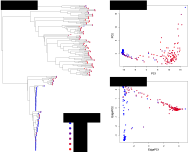
\includegraphics[width=\linewidth]{squash_edgepca.pdf}
    \begin{subfigure}{0pt}
        \phantomcaption
        \label{fig:squash_edgepca:sub:squash}
    \end{subfigure}
    \begin{subfigure}{0pt}
        \phantomcaption
        \label{fig:squash_edgepca:sub:pca}
    \end{subfigure}
    \begin{subfigure}{0pt}
        \phantomcaption
        \label{fig:squash_edgepca:sub:epca}
    \end{subfigure}
    \caption[Existing analysis methods on the BV dataset]{
        \textbf{Existing analysis methods on the BV dataset.}
        We applied \subref{fig:squash_edgepca:sub:squash} Squash Clustering,
        \subref{fig:squash_edgepca:sub:pca} PCA on the pairwise KR distance matrix between samples,
        and \subref{fig:squash_edgepca:sub:epca} Edge PCA,
        using the \acf{BV} dataset \cite{Srinivasan2012}.
        The Subfigures are recalculations of Figure~1(A) of \cite{Srinivasan2012},
        and Figures~4 and 3 of \cite{Matsen2011b}, respectively.
        All Subfigures represent samples as colored dots according to their respective Nugent score,
        which indicates the severeness of the \ac{BV} infection of the samples/patients.
%         In \subref{fig:squash_edgepca:sub:squash}, we added coloring to the samples (tips) of the cluster tree for convenience.
        See \secref{ch:Foundations:sec:PhylogeneticPlacement:sub:ExistingMethods} for a description of the methods,
        and \appref{supp:sec:DetailsEmpiricalDatasets:sub:BV} for details on the dataset.
    }
    \label{fig:squash_edgepca}
\end{figure}

Furthermore, depending on the data and research question at hand,
the KR distance is not always the best measure of sample similarity.
As explained in \secref{ch:Foundations:sec:PhylogeneticPlacement:sub:PlacementProcessing},
edge imbalances can often reveal more subtle differences between samples than edge masses.
Thus, for some datasets, it might make sense to use a distance based on edge imbalances instead.

To further illustrate this, \figref{fig:squash_edgepca:sub:pca} shows
the result of a standard principal component analysis (PCA) \cite{Pearson1901,Jolliffe2002}
on the pairwise KR distance matrix of the \acf{BV} dataset \cite{Srinivasan2012} that we used before.
On the left hand side of the figure, the blue samples,
representing healthy women with a low Nugent score, form a dense cluster.
Towards the right hand side however, the red samples, which belong to sick patients, are spread over the rest of the graph.
As Squash Clustering also uses the KR distance, the same pattern can be observed in its resulting clustering tree,
as shown in \figref{fig:squash_edgepca:sub:squash}:
The bottom half of the clustering tree, containing mainly healthy (blue) samples, has short branches,
which correspond to the dense blue region in \figref{fig:squash_edgepca:sub:pca}.
At the same time, the top half, with mostly samples from sick (red) patients, has many long branches,
corresponding to the scattered red region in \figref{fig:squash_edgepca:sub:pca}.
Thus, Squash Clustering represents equivalent information to a standard PCA on this dataset.
It thus ``suffers'' from the same shortcomings that Edge PCA is solving by using mass imbalance instead
(see \secref{ch:Foundations:sec:PhylogeneticPlacement:sub:ExistingMethods:par:EdgePCA}).
This can be seen in \figref{fig:squash_edgepca:sub:epca}, which shows the result of Edge PCA on the dataset.
There, the healthy (blue) samples clearly separate
into two groups for the two dominant \taxonname{Lactobacillus} clades in healthy patients,
which is due to the edge imbalances resolving smaller differences between the placements on nearby clades in this dataset.
Hence, for this dataset, instead of using a distance based on edge masses such as the KR distance,
edge imbalances should be used to measure distances between samples.

% ######################################################################################################################
%         Methods and Implementation
% ######################################################################################################################

\section{Methods and Implementation}
\label{ch:Clustering:sec:Methods}

We here propose two variants of $k$-means clustering \cite{Steinhaus1956,Macqueen1967},
which we call \emph{Phylogenetic $k$-means}, and \emph{Imbalance $k$-means}, respectively.
They are clustering methods for phylogenetic placement of a set of metagenomic sequence samples,
and address the issues described above.
Note that these methods are clustering samples, and not single sequences \cite{Kelley2010}.
Both methods produce a predefined number of clusters, and hence are able to work with arbitrarily large datasets.
Phylogenetic $k$-means uses the KR distance to assess sample similarity, that is, it uses edge masses,
while Imbalance $k$-means uses edge imbalances instead.

The methods take as input a set of $n$ samples, each consisting of their \acfp{QS} placed on a fixed \acf{RT}.
They then assign the samples to $k$ clusters, each represented by a cluster \emph{centroid}
that describes the average placement mass distribution of the samples assigned to it.
We later also discuss how to chose a reasonable value for $k$.

% ======================================================================================================================
%     Phylogenetic k-means
% ======================================================================================================================

% PDF bookmarks do not accept the $k$ math mode, so make it use the letter instead.
\subsection{Phylogenetic \texorpdfstring{$k$-means}{k-means}}
\label{ch:Clustering:sec:Methods:sub:PhylogeneticKmeans}

Phylogenetic $k$-means employs the KR distance (see \secref{ch:Foundations:sec:PhylogeneticPlacement:sub:Distances:par:KR})
and hence yields results that are consistent with the clustering tree of Squash Clustering.
% but it yields a predefined number of $k$ clusters.

% ----------------------------------------------------------------------------------------------------------------------
%     Algorithm
% ----------------------------------------------------------------------------------------------------------------------

\paragraph{Algorithm}
\label{ch:Clustering:sec:Methods:sub:PhylogeneticKmeans:par:Algorithm}

% The underlying idea is to assign each of the $n$ samples to one of $k$ cluster centroids,
% where each centroid represents the average mass distribution of all samples assigned to it.

The input samples and the cluster centroids are of the same data type,
namely, they are mass distributions on a fixed \ac{RT}.
It is thus possible to calculate the KR distances between samples and centroids,
and to calculate their average mass distributions by \emph{squashing},
as described in \secref{ch:Foundations:sec:PhylogeneticPlacement:sub:PlacementProcessing:par:EdgeMasses}.

The objective is then to find an assignment of the $n$ samples into $k$ clusters
that minimizes the total distance between each sample and the cluster centroid it is assigned to,
measured as the KR distance between them.
That is, for $k$ clusters, each represented by a set $A_k$ of samples assigned to it, and its centroid $C_k$,
the objective is to find

\begin{equation}
    \label{ch:Clustering:eq:KmeansObjective}
    \hat{A} ~=~ \argmin_A \sum_{i=1}^{k} \sum_{s \in A_i} \mbox{KR}( s, C_i )
\end{equation}

% Keep in mind that each sample in the assignments $A_k$ and each centroid $C_k$
% are placement mass distributions on the \ac{RT}, between which the KR distance can be calculated.
The optimal solution $\hat{A}$ for the assignment of samples to clusters can be found via a brute-force search.
However, the number of possible assignments of $n$ samples to $k$ clusters
is given by the Stirling partition number $S(n,k)$ \cite{Graham1989a},
which is too large for any realistic dataset.

Hence, our implementation follows the Lloyd-Forgy algorithm \cite{Lloyd1982,Forgy1965},
which is the standard heuristical method to solve the $k$-means problem.
It iteratively improves the assignments $A$ and the centroids $C$ in two alternating steps,
as shown in \algref{algo:kmeans}.

% \todo{maybe remove space later again:}
% \vspace*{1em}
\begin{algorithm}
\caption{Phylogenetic $k$-means}\label{algo:kmeans}
\begin{algorithmic}[1]
    \State initialize $k$ \textit{Centroids}
    \While{not converged}
        \State assign each \textit{Sample} to nearest \textit{Centroid} ($A$)
        \State update \textit{Centroids} as mass averages of their \textit{Samples} ($C$)
    \EndWhile
    \State \textbf{return} \textit{Assignments} $A$ and \textit{Centroids} $C$
\end{algorithmic}
\end{algorithm}

By default, we use the $k$-means++ initialization algorithm \cite{Arthur2007} to obtain an initial set of $k$ centroids.
It works by subsequent random selection of samples to be used as initial centroids,
until $k$ centroids have been selected.
In each step, the probability of selecting a sample is
proportional to its squared distance to the nearest already selected sample.
Hence, centroids are preferably selected that are far away from each other.
An alternative initialization is to select samples as initial clusters entirely at random.
This is however more likely to yield sub-optimal clusterings \cite{Kanungo2003}.

Then, each sample is assigned to its nearest centroid, using the KR distance. %for example the KR or NH distance.
Lastly, the centroids are updated to represent
the average mass distribution of all samples that are currently assigned to them.
This iterative process alternates between improving the assignments and the centroids.
Thus, the main difference to normal $k$-means in the $\mathbb{R}^d$ is the use of phylogenetic information:
Instead of euclidean distances on vectors, we use the KR distance,
and instead of averaging vectors to obtain centroids, we use the average mass distribution.

The process is repeated until it converges,
that is, the cluster assignments do not change any more between subsequent iterations,
or until a maximum number of iterations have been executed.
% The second stopping criterion makes sure that the algorithm terminates even with non-convergent datasets.
This second stopping criterion is added to avoid the super-polynomial worst case running time of $k$-means,
which however almost never occurs in practice \cite{Bottou1995,Arthur2006}.

The result of the algorithm is an assignment of each sample to one of the $k$ clusters.
As the algorithm relies on the KR distance, it clusters samples with similar relative abundances.
The cluster centroids can be visualized as trees with a mass distribution,
analogous to how Squash Clustering visualizes inner nodes of the clustering tree.
That is, each centroid can be represented as the average mass distribution of the samples that were assigned to it.
This allows to inspect the centroids and thus to interpret how the samples were clustered.
% For instance, the diversity and taxonomic assignment of the centroids represents the corresponding sets of samples.
Examples of this are shown in \figref{fig:centroids}.

% ----------------------------------------------------------------------------------------------------------------------
%     Algorithmic Improvements
% ----------------------------------------------------------------------------------------------------------------------

\paragraph{Algorithmic Improvements}
\label{ch:Clustering:sec:Methods:sub:PhylogeneticKmeans:par:AlgorithmicImprovements}

In each assignment step of the algorithm, distances from all samples to all centroids are calculated,
which has a time complexity of $\mathcal{O}(n \cdot k)$.
In order to accelerate this step, we can apply branch binning
as introduced in \secref{ch:Foundations:sec:PhylogeneticPlacement:sub:PlacementProcessing:par:EdgeMasses}.
For the \ac{BV} dataset, we found that even using just \num{2} bins per edge does not alter the cluster assignments.
Branch binning reduces the number of mass points that have to be accessed in memory during KR distance calculations;
however, the costs for tree traversals remain.
Thus, we observed a maximal speedup of 75\% when using one bin per branch,
see \tabref{tab:hmp_binning_error} for details.
Intermediate binning strategies are also possible:
instead of binning all masses of the input samples, just the centroid masses can be binned.

% even binning to \num{1} bin,
% that is, combining all placement masses on a branch into one point,
% changes the cluster assignment of only \num{2} of {220} samples
% -- both of which were near the border between two clusters.
% The main bottleneck in the computation however seems to be
% the random memory access to the edges and per-edge masses induced by the tree traversals
% so that binning does not yield substantial speedups.
% In our tests, summarizing all masses in one bin per branch resulted in a speedup of around 75\%,

Furthermore, during the execution of the algorithm, empty clusters can occur,
for example, if $k$ is greater than the number of natural clusters in the data.
Although this problem did not occur in our tests, we implemented the following solution:
First, find the cluster with the highest variance.
Then, choose the sample of that cluster that is furthest from its centroid,
and assign it to the empty cluster instead.
This process is repeated if multiple empty clusters occur at once.

% ======================================================================================================================
%         Imbalance k-means
% ======================================================================================================================

% PDF bookmarks do not accept the $k$ math mode, so make it use the letter instead.
\subsection{Imbalance \texorpdfstring{$k$-means}{k-means}}
\label{ch:Clustering:sec:Methods:sub:ImbalanceKmeans}

We further propose \emph{Imbalance $k$-means},
which is a variant of $k$-means that makes use of the edge imbalance transformation
(see \secref{ch:Foundations:sec:PhylogeneticPlacement:sub:PlacementProcessing:par:EdgeImbalances}),
and thus takes the clades of the reference tree into account.
In order to quantify the difference in imbalances between two samples,
we use the euclidean distance between their imbalance vectors (that is, rows of the imbalance matrix).
This is a suitable distance measure,
as the imbalances implicitly capture the tree topology as well as the placement mass distributions.
As a consequence, the expensive tree traversals required for Phylogenetic $k$-means are not necessary for the calculations.
The algorithm takes the edge imbalance matrix of normalized samples as input,
% as shown in \figref{fig:imbalance:sub:Matrices},
and performs a standard euclidean $k$-means clustering following the Lloyd-Forgy algorithm \cite{Lloyd1982,Forgy1965}.
% As there is no apparent phylogenetically informative distance measure between imbalance vectors,
% we use euclidean distance instead.
% This also allows to calculated centroids as simple vector averages.

This variant of $k$-means tends to find clusters that are consistent with the results of Edge PCA,
as both use the same input data and both operate in euclidean space. %as well as the same distance measure.
Furthermore, as the method does not need to calculate KR distances,
and thus neither involves tree traversals nor needs to consider each placement location (or bins of those) separately,
it is several orders of magnitude faster than Phylogenetic $k$-means.
For example, on the \ac{HMP} dataset (see \appref{supp:sec:DetailsEmpiricalDatasets:sub:HMP}),
it runs in mere seconds, instead of several hours needed for Phylogenetic $k$-means;
see Section \secref{ch:Clustering:sec:Results:sub:Performance} for details.

% ======================================================================================================================
%     Finding k
% ======================================================================================================================

\subsection{Finding appropriate values for \texorpdfstring{$k$}{k}}
\label{ch:Clustering:sec:Methods:sub:FindingK}

A commonly criticized downside of $k$-means clustering in general is
that the number of clusters $k$ is an input parameter to the algorithm.
Hence, a key question is how to select an appropriate $k$
that reflects the number of ``natural'' clusters in the data.
There exist various suggestions in the literature
\cite{Thorndike1953,Rousseeuw1987,Bischof1999,Pelleg2000,Tibshirani2001,Hamerly2004}.
% See also: https://stackoverflow.com/a/1793572/4184258 and
% http://www.sthda.com/english/articles/29-cluster-validation-essentials/96-determining-the-optimal-number-of-clusters-3-must-know-methods/

We evaluated the Elbow method \cite{Thorndike1953},
which is a straight forward method that yielded reasonable results for our test datasets.
It works by plotting the cluster variance,
that is, the average squared distance of the samples to their assigned cluster centroids,
for different values of $k$.
On the one hand, for low values of $k$, many samples exhibit a large distance to their assigned centroid,
% the distances from samples to their assigned centroids are relatively
inducing a high variance.
On the other hand, higher values of $k$ further split the clusters and hence reduce the variance.
% and slightly reduce this distance by further splitting clusters.
Thus, at a given point, increasing $k$ only yields a marginal change in variance.
If the data has a natural number of clusters, the corresponding $k$ at this point produces an angle in the plot,
called the \emph{elbow}.
Thus, the presence of an elbow in the variance plot indicates reasonable values for $k$.

Additionally, for a quantitative evaluation of the clusterings,
we used the $k$ that arose from the number of distinct categories or labels based on the available meta-data for the data.
% that is, the number of distinct categories our data is known to belong to.
For example, the samples of the \ac{HMP} dataset are labeled with \num{18} distinct body sites,
describing where each sample was taken from, c.f.~\figref{fig:hmp_kmeans_all_18}.

% ######################################################################################################################
%         Results
% ######################################################################################################################

\section{Evaluation and Results}
\label{ch:Clustering:sec:Results}

We here evaluate the two $k$-means variants in terms of their clustering accuracy and performance.
We used the \acf{BV} dataset (see \appref{supp:sec:DetailsEmpiricalDatasets:sub:BV} for details)
as an example of a small dataset to which methods such as Squash Clustering \cite{Matsen2011a}
are still applicable for comparison,
and the \acf{HMP} dataset (see \appref{supp:sec:DetailsEmpiricalDatasets:sub:HMP})
to showcase that our methods scale to datasets that are too large for existing methods.

% ======================================================================================================================
%     BV Dataset
% ======================================================================================================================

\subsection{BV Dataset}
\label{ch:Clustering:sec:Results:sub:BVDataset}

We placed the samples of the \ac{BV} dataset \cite{Srinivasan2012}
on the re-inferred reference tree of their original reference sequences
to test whether our methods work as expected.
To this end, we ran both Phylogenetic $k$-means and Imbalance $k$-means on the \ac{BV} dataset,
and compare the results to the existing analysis of the data in \cite{Srinivasan2012} and \cite{Matsen2011a}.
We chose $k:=3$, inspired by the findings of \cite{Srinivasan2012}.
There, they distinguish between subjects affected by Bacterial Vaginosis and healthy subjects,
and further separate the healthy ones into two categories depending on the dominating clade in the vaginal microbiome,
which is either \taxonname{Lactobacillus iners} or \taxonname{Lactobacillus crispatus}.
Any choice of $k > 3$ would simply result in smaller, more fine-grained clusters,
but not change the general findings of these experiments.
The number of clusters is also evaluated using the Elbow method later in \secref{ch:Clustering:sec:Results:sub:ElbowMethod}.

For each of the \num{220} samples of the dataset, we hence obtained two cluster assignments:
First, by using Phylogenetic $k$-means, we obtained the cluster assignment \emph{PKM}.
Second, by using Imbalance $k$-means, we obtained assignment \emph{IKM}.
In the following figures, the samples are represented by colored circles:
red, green, and blue show the cluster assignments \emph{PKM},
while purple, orange, and gray show the cluster assignments \emph{IKM}.
We use two different color sets for the two methods, in order to make them distinguishable at first glance.
Note that the mapping of colors to clusters is arbitrary and depends on the random initialization of the algorithm.

We then conducted Squash Clustering and Edge PCA (\secref{ch:Foundations:sec:PhylogeneticPlacement:sub:ExistingMethods})
on the dataset, thereby reproducing results of previous studies,
as well as two alternative dimensionality reduction methods.
This allows for a direct comparison between our novel and the existing methods.

% The figure shows the results of Squash Clustering, Edge PCA, and two alternative dimensionality reduction methods,
% colorized by the cluster assignments \emph{PKM} of Phylogenetic $k$-means (in red, green, and blue)
% and \emph{IKM} of the Imbalance $k$-means (in purple, orange, and gray), respectively.

% ----------------------------------------------------------------------------------------------------------------------
%     Squash Clustering
% ----------------------------------------------------------------------------------------------------------------------

\paragraph{Comparison to Squash Clustering}
\label{ch:Clustering:sec:Results:sub:BVDataset:par:SquashClustering}

\begin{figure}[p]
    \centering
    \includegraphics[width=\linewidth]{cluster_kmeans_trees.pdf}
    \begin{subfigure}{0pt}
        \phantomcaption
        \label{fig:cluster_kmeans_trees:sub:mass_tree}
    \end{subfigure}
    \begin{subfigure}{0pt}
        \phantomcaption
        \label{fig:cluster_kmeans_trees:sub:imbalance_tree}
    \end{subfigure}
    \caption[Comparison of $k$-means clustering to Squash Clustering]{
        \textbf{Comparison of $k$-means clustering to Squash Clustering.}
        We applied Squash Clustering to the \ac{BV} dataset \cite{Srinivasan2012},
        to compare it to the assignments obtained from our $k$-means variants.
        % in order to compare them to existing methods.
%         See \cite{Srinivasan2012} for details of the dataset and its interpretation.
%         We chose $k:=3$, as this best fits the features of the dataset.
        % Sub (A)
        \subref{fig:cluster_kmeans_trees:sub:mass_tree}
        Hierarchical cluster tree of the samples, using Squash Clustering.
        The tree is a recalculation of Figure~1(A) of \cite{Srinivasan2012}.
        Each leaf represents a sample; branch lengths are KR distances.
        We added color coding for the samples, using \emph{PKM}.
        The lower half of red samples are mostly healthy subjects,
        while the green and blue upper half are patients affected by Bacterial Vaginosis.
        % Sub (B)
        \subref{fig:cluster_kmeans_trees:sub:imbalance_tree}
        The same tree, but annotated by \emph{IKM}.
        The tree is flipped horizontally for ease of comparison.
        The healthy subjects are split into two sub-classes,
        discriminated by the dominating species in their vaginal microbiome:
        orange and purple represent samples were \taxonname{Lactobacillus iners} and \taxonname{Lactobacillus crispatus}
        dominate the microbiome, respectively.
        The patients mostly affected by BV are clustered in gray.
    }
    \label{fig:cluster_kmeans_trees}
\end{figure}

The comparison of our $k$-means clustering assignments to Squash Clustering is shown in \figref{fig:cluster_kmeans_trees}.
As can be seen in \figref{fig:cluster_kmeans_trees:sub:mass_tree}, Squash Clustering as well as
Phylogenetic $k$-means can distinguish healthy subjects from those affected by Bacterial Vaginosis.
Healthy subjects constitute the lower part of the cluster tree.
They have shorter branches between each other, indicating the smaller KR distance between them,
which is a result of the dominance of \taxonname{Lactobacillus} in healthy subjects.
The same clusters are found by Phylogenetic $k$-means:
As it uses the KR distance, it assigns all healthy subjects to one cluster (shown in red),
which is consistent with the short cluster tree branches in \figref{fig:cluster_kmeans_trees:sub:mass_tree}.
The green and blue clusters are mostly the subjects affected by the disease.

In \figref{fig:cluster_kmeans_trees:sub:imbalance_tree}, we compare Squash Clustering to Imbalance $k$-means.
Here, the distinction between the two \taxonname{Lactobacillus} clades
can be seen by the purple and orange cluster assignments.
The cluster tree also separates those clusters into two clades.
The separate small group of orange samples above the purple clade is an artifact of the tree visualization (ladderization),
and actually is close to the other orange samples below.
The diseased subjects are all assigned to the gray cluster, represented by the upper half of the cluster tree.
It is apparent that both methods separate the same samples from each other.

% ----------------------------------------------------------------------------------------------------------------------
%     Edge PCA
% ----------------------------------------------------------------------------------------------------------------------

\paragraph{Comparison to Edge PCA}
\label{ch:Clustering:sec:Results:sub:BVDataset:par:EdgePCA}

\begin{figure}[p]
    \centering
    \includegraphics[width=\linewidth]{kmeans_all.pdf}
    \begin{subfigure}{0pt}
        \phantomcaption
        \label{fig:kmeans_all:sub:mds_em}
    \end{subfigure}
    \begin{subfigure}{0pt}
        \phantomcaption
        \label{fig:kmeans_all:sub:mds_ei}
    \end{subfigure}
    \begin{subfigure}{0pt}
        \phantomcaption
        \label{fig:kmeans_all:sub:mds_ns}
    \end{subfigure}
    \begin{subfigure}{0pt}
        \phantomcaption
        \label{fig:kmeans_all:sub:pca_em}
    \end{subfigure}
    \begin{subfigure}{0pt}
        \phantomcaption
        \label{fig:kmeans_all:sub:pca_ei}
    \end{subfigure}
    \begin{subfigure}{0pt}
        \phantomcaption
        \label{fig:kmeans_all:sub:pca_ns}
    \end{subfigure}
    \begin{subfigure}{0pt}
        \phantomcaption
        \label{fig:kmeans_all:sub:epca_em}
    \end{subfigure}
    \begin{subfigure}{0pt}
        \phantomcaption
        \label{fig:kmeans_all:sub:epca_ei}
    \end{subfigure}
    \begin{subfigure}{0pt}
        \phantomcaption
        \label{fig:kmeans_all:sub:epca_ns}
    \end{subfigure}
    \caption[Comparison of $k$-means clustering to MDS, PCA, and Edge PCA]{
        \textbf{Comparison of $k$-means clustering to MDS, PCA, and Edge PCA.}
        Here, we show the dimensionality reduction methods MDS, PCA, and Edge PCA (one per row) on the \ac{BV} dataset.
        MDS and PCA were calculated on the pairwise KR distance matrix of the samples,
        Edge PCA was calculated using the placements on the re-inferred \ac{RT} of the original publication \cite{Srinivasan2012}.
        The plots are colored by the cluster assignments \emph{PKM} and \emph{IKM}
        as found by our $k$-means variants (first two columns), and by the Nugent score of the samples (third column).
        The Nugent score is included to allow comparison of the health status of patients with the clustering results.
        \subref{fig:kmeans_all:sub:pca_ns} and \subref{fig:kmeans_all:sub:epca_ns} are recalculations of
        Figures~4 and 3 of \cite{Matsen2011b}, respectively.
    }
    \label{fig:kmeans_all}
\end{figure}

In \figref{fig:kmeans_all}, we compare the assignments obtained from our $k$-means variants
to several dimensionality reduction methods, such as Edge PCA.
The figure reveals additional details about how the $k$-means method works,
that is, which samples are assigned to the same cluster.

The first row of \figref{fig:kmeans_all} shows the result of
\acf{MDS} of the pairwise KR distance matrix between the samples.
\ac{MDS} \cite{Mardia1978,Krzanowski1994,Everitt2010} is a dimensionality reduction method that
can be used for visualizing levels of similarity between data points.
Given a pairwise distance matrix, it finds an embedding into lower dimensions (in this case, \num{2} dimensions)
that preserves higher dimensional distances as well as possible.

The distinguishing features between the green and the blue cluster
are not apparent in the Squash cluster tree in \figref{fig:cluster_kmeans_trees:sub:mass_tree}.
This can however be seen in \figref{fig:kmeans_all:sub:mds_em}, which shows the \ac{MDS} plot colored by \emph{PKM}.
Here, the red cluster forms a dense region, which is in agreement with the short branch lengths
in the cluster tree of \figref{fig:cluster_kmeans_trees:sub:mass_tree}.
At the same time, the green and blue cluster are separated in the \ac{MDS} plot,
but form a coherent region of low density,
indicating that $k:=3$ might be too large when applying Phylogenetic $k$-means to this dataset.
That is, the actual clustering just distinguishes healthy from sick patients (c.\,f.~\figref{fig:elbows}),
meaning that \num{2} dimensions might also suffice here.
% which, albeit not well separated from each other, indicate groups of samples with lower KR distance between each other.
Although the separation between green and blue samples is smooth,
it shows that Phylogenetic $k$-means finds clusters based on KR distance between samples,
and thus yields results consistent with Squash Clustering and \ac{MDS}.

A similar visualization of the pairwise KR distances is shown in the second row of \figref{fig:kmeans_all},
where we applied standard \acf{PCA} \cite{Krzanowski1994,Everitt2010} to the pairwise KR distance matrix
by interpreting it as a data matrix.
Although it is mathematically sound, the direct application of \ac{PCA} to a distance matrix lacks a simple interpretation,
which was previously used to motivate Edge PCA
(c.\,f.~\secref{ch:Foundations:sec:PhylogeneticPlacement:sub:ExistingMethods:par:EdgePCA}).
Still, this can be seen as a visualization of the distances that helps understanding our methods.

For example, in \figref{fig:kmeans_all:sub:pca_em},
% It is a recalculation of Figure~4 in the preprint \cite{Matsen2011b},
% which did not appear in the final published version \cite{Matsen2011a}.
% It is a recalculation of Figure~4 of \cite{Matsen2011b}.
% but can also be found at \cite{MatsenEdgePCA}.
which shows the PCA plot colored by \emph{PKM}, the red cluster again is clearly separated from the rest.
This time however, the distinction between the green and the blue cluster
is not as apparent as in \figref{fig:kmeans_all:sub:mds_em}.

Furthermore, \figref{fig:kmeans_all:sub:mds_ei} and \subref{fig:kmeans_all:sub:pca_ei} show the MDS and the PCA plot,
respectively, this time colored by \emph{IKM}.
Here, the purple cluster found by Imbalance $k$-means forms a dense cluster of close-by samples on the left of the plots,
which is in accordance with the short branch lengths
of this cluster as shown in the clustering tree in \figref{fig:cluster_kmeans_trees:sub:imbalance_tree}.
The orange cluster is slightly more spread out in the plots,
which again can be seen by the longer branch lengths in \figref{fig:cluster_kmeans_trees:sub:imbalance_tree}.

Finally, we applied Edge PCA to the samples, as shown in the last row of \figref{fig:kmeans_all}.
In particular, \figref{fig:kmeans_all:sub:epca_ei} compares Imbalance $k$-means to Edge PCA
by coloring the plot using \emph{IKM}.
% The plot is a recalculation of Figure~3 of \cite{Matsen2011b}, which also appeared in Figure~6 in \cite{Matsen2011a}
% and Figure~3 in \cite{Srinivasan2012},
Because both methods work on edge imbalances, they group the data in the same way, and are thus consistent with each other.
That is, they clearly separate the two healthy groups and the diseased one from each other.
Edge PCA forms a plot with three corners, which are colored by the three Imbalance $k$-means cluster assignments.

% ----------------------------------------------------------------------------------------------------------------------
%     Cluster Centroids
% ----------------------------------------------------------------------------------------------------------------------

\paragraph{Cluster Centroids}
\label{ch:Clustering:sec:Results:sub:BVDataset:par:ClusterCentroids}

As mentioned before, an advantage of using phylogenetic placements as input to our $k$-means clustering methods
is the ability to visualize cluster centroids by showing the average mass distribution
of the samples assigned to them on the underlying \acf{RT}.
In Phylogenetic $k$-means, the mass distributions of the centroids are already part of the algorithm,
as they are needed for calculating the KR distances between samples and centroids.
In Imbalance $k$-means however, the placement data is used in form of edge imbalances instead of masses.
Still, after convergence of the algorithm, the per-centroid average mass can be calculated from the input samples
and again visualized on the \ac{RT}.

\begin{figure}[!tb]
    \centering
    \includegraphics[width=\linewidth]{centroids.pdf}
    \begin{subfigure}{0pt}
        \phantomcaption
        \label{fig:centroids:sub:red}
    \end{subfigure}
    \begin{subfigure}{0pt}
        \phantomcaption
        \label{fig:centroids:sub:green}
    \end{subfigure}
    \begin{subfigure}{0pt}
        \phantomcaption
        \label{fig:centroids:sub:blue}
    \end{subfigure}
    \begin{subfigure}{0pt}
        \phantomcaption
        \label{fig:centroids:sub:purple}
    \end{subfigure}
    \begin{subfigure}{0pt}
        \phantomcaption
        \label{fig:centroids:sub:orange}
    \end{subfigure}
    \begin{subfigure}{0pt}
        \phantomcaption
        \label{fig:centroids:sub:gray}
    \end{subfigure}
    \caption[Example of $k$-means cluster centroids visualization]{
        % In this figure, I assume that the reader is already familiar with the characteristics of the dataset.
        % No need to repeat everything over again...
        \textbf{Example of $k$-means cluster centroids visualization.}
        Here we show the cluster centroids as found by our $k$-means variants using the \ac{BV} dataset,
        visualized on the reference tree via color coding.
        The cluster assignments are the same as in \figref{fig:cluster_kmeans_trees} and \figref{fig:kmeans_all};
        the first row show the three clusters found by Phylogenetic $k$-means,
        the second row the clusters found by Imbalance $k$-means.
        Each tree represents one centroid around which the samples were clustered,
        that is, it shows the combined masses of the samples that were assigned to that cluster.
        The edges are colored relative to each other, using a linear scaling of
        light blue (no mass), purple (half of the maximal mass) and black (maximal mass).
        The two \taxonname{Lactobacillus} clades are marked with black arcs on the left of the trees.
    }
    \label{fig:centroids}
\end{figure}

Examples of this are shown in \figref{fig:centroids},
for both sample assignments \emph{PKM} (first row) and \emph{IKM} (second row) of the \ac{BV} dataset.
As explained above, the samples can be split into three groups:
The diseased subjects, which have placement mass in various parts of the tree,
as well as two groups of healthy subjects, with placement mass in one of two \taxonname{Lactobacillus} clades,
marked with black arcs in \figref{fig:centroids}.
This grouping is also clearly visible in the trees.
The red cluster in \subref{fig:centroids:sub:red} for example represents all healthy subjects;
thus, most of its mass is located in the two \taxonname{Lactobacillus} clades.
The purple and orange clusters in \subref{fig:centroids:sub:purple} and \subref{fig:centroids:sub:orange}
on the other hand show a difference in placement mass between those clades.
Furthermore, the placement mass of the gray cluster in \subref{fig:centroids:sub:gray} is mostly
a combination of the masses of the green and blue cluster in \subref{fig:centroids:sub:green} and \subref{fig:centroids:sub:blue},
all of which represent diseased subjects.
These observations are in accordance with the previous findings above,
and further support that our methods yield results that are in agreement with existing methods.
% In summary, our novel $k$-means variants find clusters that are in agreement with existing methods.

% ======================================================================================================================
%     HMP Dataset
% ======================================================================================================================

\subsection{HMP Dataset}
\label{ch:Clustering:sec:Results:sub:HMPDataset}

The \acf{HMP} dataset \cite{Huttenhower2012,Methe2012} (see \appref{supp:sec:DetailsEmpiricalDatasets:sub:HMP} for details)
is used here as an example to show that our method scales to large datasets.
To this end, we used the unconstrained \taxonname{Bacteria} \ac{RT} with \num{1 914} taxa
obtained from our \ac{PhAT} method, see \secref{ch:AutomaticTrees:sec:Evaluation:sub:ReferenceTreeSetup} for details.
% as provided by our Automatic Reference Tree method \cite{Czech2018}.
The tree represents a broad taxonomic range of \taxonname{Bacteria},
that is, the sequences were \emph{not} explicitly selected for the \ac{HMP} dataset,
in order to test the robustness of our clustering methods.
We then placed the \num{9 192} samples of the \ac{HMP} dataset with a total of \num{118 701 818} sequences on that tree,
and calculated Phylogenetic and Imbalance $k$-means on the samples.

The freely available meta-data for the \ac{HMP} dataset labels each sample by the body site were it was taken from.
As there are \num{18} different body site labels, we used $k:=18$.
The resulting clustering assignments are shown in \figref{fig:hmp_kmeans_all_18}.
Furthermore, in \figref{fig:hmp_kmeans_all_8},
we show a clustering of this dataset into $k:=8$ broader body site groups
to exemplify the effect of using different values of $k$.
See \tabref{tab:hmp_data_overview} for the grouping of the original body site labels.
The effect of $k$ on the clustering results is further explored by using the Elbow method,
as described later in \secref{ch:Clustering:sec:Results:sub:ElbowMethod}.
% that is, using the constrained Bacterial tree as well as Imbalance $k$-means.

\begin{figure}[hpbt]
    \centering
    \includegraphics[width=\linewidth]{hmp_kmeans_all_18.pdf}
    \begin{subfigure}{0pt}
        \phantomcaption
        \label{fig:hmp_kmeans_all_18:sub:em_unconstr}
    \end{subfigure}
    \begin{subfigure}{0pt}
        \phantomcaption
        \label{fig:hmp_kmeans_all_18:sub:ei_unconstr}
    \end{subfigure}
    \caption[$k$-means cluster assignments of the \acs{HMP} dataset with $k:=18$]{
        \textbf{$k$-means cluster assignments of the \acs{HMP} dataset with $k:=18$.}
        Here, we show the cluster assignments as yielded by
        \subref{fig:hmp_kmeans_all_18:sub:em_unconstr} Phylogenetic $k$-means and
        \subref{fig:hmp_kmeans_all_18:sub:ei_unconstr} Imbalance $k$-means on the \ac{HMP} dataset.
        We used $k:=18$, which is the number of body site labels in the dataset,
        in order to compare the clusterings to this ``ground truth''.
        Each row represents a body site; each column one of the 18 clusters found by the algorithm.
        We also show a translation of the body site labels into the corresponding body regions.
        The color values indicate how many samples of a body site are assigned to each cluster.
        Similar body sites are clearly grouped together in coherent blocks, indicated by darker colors.
        For example, the stool samples are split into two clusters (topmost row),
        while the three vaginal sites are all put into one cluster (rightmost column).
        However, the algorithm cannot always distinguish between nearby body sites,
        as can be seen from the fuzziness of the clusters of oral samples.
%         Lastly, the figure also lists how the body site labels were aggregated into coarse regions
%         as used in \figref{fig:hmp_kmeans_all_8}.
    }
    \label{fig:hmp_kmeans_all_18}
\end{figure}

\begin{figure}[hpbt]
    \centering
    \includegraphics[width=0.6\linewidth]{hmp_kmeans_all_8.pdf}
    \begin{subfigure}{0pt}
        \phantomcaption
        \label{fig:hmp_kmeans_all_8:sub:em_unconstr}
    \end{subfigure}
    \begin{subfigure}{0pt}
        \phantomcaption
        \label{fig:hmp_kmeans_all_8:sub:ei_unconstr}
    \end{subfigure}
    \caption[$k$-means cluster assignments of the \acs{HMP} dataset with $k:=8$]{
        \textbf{$k$-means cluster assignments of the \acs{HMP} dataset with $k:=8$.}
        Here, we again show the cluster assignments as yielded by
        \subref{fig:hmp_kmeans_all_8:sub:em_unconstr} Phylogenetic $k$-means and
        \subref{fig:hmp_kmeans_all_8:sub:ei_unconstr} Imbalance $k$-means on the \ac{HMP} dataset,
        but with $k$ being set to 8, instead of $k:=18$ as in \figref{fig:hmp_kmeans_all_18}.
        These \num{8} clusters are based on an aggregation of the original body site labels into groups,
        as shown in \tabref{tab:hmp_data_overview}.
%         for the list of how the original body site labels were aggregated.
        %for the cluster assignment where $k$ is set to the original number of labels;
        Each row represents a body group; each column one of the \num{8} clusters found by the algorithm.
%         The color values indicate how many samples of a body site were assigned to each cluster.
        Some of the body sites are again clearly separated,
        while particularly the samples from the oral region are distributed over different clusters.
%         This might be due to %the broad reference tree not being able to resolve the fine details between these samples,
%         but might also indicate a
%         homogeneity of the oral samples.
    }
    \label{fig:hmp_kmeans_all_8}
\end{figure}

% Ideally, each cluster would contain only samples from the same body site.
Ideally, all samples from one body site would be assigned to the same cluster,
hence forming a diagonal in the plots of \figref{fig:hmp_kmeans_all_18} and \figref{fig:hmp_kmeans_all_8}.
However, as there are several nearby body sites, which share a large fraction of their microbiome \cite{Huttenhower2012},
we do not expect a perfect clustering.
Furthermore, we used a broad reference tree that might not be able to resolve details in some clades.
% which was originally meant only for a first classification of sequences (see above).
% Thus, the tree does not particularly suit the dataset well.
Nonetheless, the clustering is reasonable, which indicates a robustness against the exact choice of reference taxa.
% and can thus be used for distinguishing among samples.

The plots of the two $k$-means variants generally exhibit similar characteristics in \figref{fig:hmp_kmeans_all_18}.
Most prominently, the stool and vaginal samples are clearly clustered into coherent blocks in both variants.
There are however also some differences.
For example, the samples from the body surface (arm, nose, and ear)
form two relatively dense clusters (columns) in \figref{fig:hmp_kmeans_all_18:sub:em_unconstr},
whereas those sites are spread across four or five clusters in \figref{fig:hmp_kmeans_all_18:sub:ei_unconstr}.
% In general however, these samples form two blocks of cluster columns in both plots.
On the other hand, the mouth samples are more densely clustered in \figref{fig:hmp_kmeans_all_18:sub:ei_unconstr}.

It is remarkable that the oral samples are mostly split into two blocks,
corresponding to the front of the mouth and its back, in both variants of $k$-means in \figref{fig:hmp_kmeans_all_18}.
This indicates that the clustering is sensitive to such subtle differences.
However, within these blocks, there is some fuzziness in the clustering.
This might be caused by our broad reference tree,
and could potentially be resolved by using a tree more specialized for the data/region.
It could however also simply be an artifact of the homogeneity of samples
taken from the close-by oral regions of the human body.

Lastly, using the two \taxonname{General} trees of our \ac{PhAT} method
as described in \secref{ch:AutomaticTrees:sec:Evaluation:sub:ReferenceTreeSetup},
we again evaluated the cluster assignments on the \ac{HMP} datasets (data not shown).
Using this even less specific set of reference taxa yielded cluster assignments
which are almost identical to the ones shown above, except for slightly more fuzziness.
We thus expect that the clustering improves when using an \ac{RT}
containing taxa specifically chosen for the type of sequences in the dataset.
% This however remains future work.

% ======================================================================================================================
%     k-means Elbow Plots
% ======================================================================================================================

\subsection{Elbow Method}
\label{ch:Clustering:sec:Results:sub:ElbowMethod}

As explained in \secref{ch:Clustering:sec:Methods:sub:FindingK},
plots of the cluster variance can be used for the Elbow method
in order to find an appropriate number of clusters in a dataset \cite{Thorndike1953}.
\figref{fig:elbows} shows these plots for our two test datasets.

\begin{figure}[hpbt!]
    \centering
    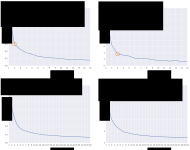
\includegraphics[width=\linewidth]{elbows.pdf}
    \begin{subfigure}{0pt}
        \phantomcaption
        \label{fig:elbows:sub:bv_phylo}
    \end{subfigure}
    \begin{subfigure}{0pt}
        \phantomcaption
        \label{fig:elbows:sub:bv_imb}
    \end{subfigure}
    \begin{subfigure}{0pt}
        \phantomcaption
        \label{fig:elbows:sub:hmp_phylo}
    \end{subfigure}
    \begin{subfigure}{0pt}
        \phantomcaption
        \label{fig:elbows:sub:hmp_imb}
    \end{subfigure}
    \caption[Variances of $k$-means clusters in our test datasets]{
        \textbf{Variances of $k$-means clusters in our test datasets.}
        The figures show the cluster variance for different values of $k$.
        The first row are clusterings of the BV dataset, the second row of the HMP dataset.
        They were clustered using Phylogenetic $k$-means (first column),
        and Imbalance $k$-means (second column), respectively.
        Accordingly, \subref{fig:elbows:sub:bv_phylo} and \subref{fig:elbows:sub:hmp_phylo} use the KR distance,
        while \subref{fig:elbows:sub:bv_imb} and \subref{fig:elbows:sub:hmp_imb} use the euclidean distance
        to measure the variance.
        Orange circles mark potential elbow points.
    }
    \label{fig:elbows}
\end{figure}

The plots for the \ac{BV} dataset in \figref{fig:elbows:sub:bv_phylo} and \subref{fig:elbows:sub:bv_imb}
exhibit the elbow at $k:=2$ and $3$, respectively, which are marked with orange circles.
% exhibit clear elbow points candidates for $k$
These values are consistent with previous findings, c.\,f. \figref{fig:cluster_kmeans_trees} and \figref{fig:kmeans_all}.
On the one hand, Phylogenetic $k$-means splits the samples into a distinct red cluster,
separated from the green and blue clusters,
effectively forming two clusters, which represent the health status of the patients.
On the other hand, Imbalance $k$-means yields three separate clusters in purple, orange, and gray,
which correspond to two clusters for the dominant \taxonname{Lactobacillus} clades,
as well as a cluster for the patients affected by \ac{BV}.

In the plots for the \ac{HMP} dataset, the elbow is less pronounced.
We suspect that this is due to two reasons, as explained in \secref{ch:Clustering:sec:Results:sub:HMPDataset}:
(i) the broad reference tree might not being able to adequately resolve fine-grained differences between samples,
and (ii) nearby body sites might simply be too homogeneous in their metagenomic composition for a clear separation into clusters.
Likely candidates for $k$ are \num{4}--\num{6} for Phylogenetic $k$-means in \figref{fig:elbows:sub:hmp_phylo}
and around \num{7} for Imbalance $k$-means in \figref{fig:elbows:sub:hmp_imb}.
These values are consistent with the number of coherent ``blocks'' of clusters,
as shown in \figref{fig:hmp_kmeans_all_18}.
Clearer results for this dataset might be obtained with other methods for finding ``good'' values for $k$,
although we did not test them here.

% ======================================================================================================================
%     Performance
% ======================================================================================================================

\subsection{Performance}
\label{ch:Clustering:sec:Results:sub:Performance}

The complexity of Phylogenetic $k$-means is in $\mathcal{O}(k \cdot i \cdot n \cdot e)$,
with $k$ clusters, $i$ iterations, and $n$ samples, and $e$ being the number of tree edges,
which corresponds to the number of dimensions in standard euclidean $k$-means.
As the centroids are randomly initialized, the number of iterations can vary;
in our tests, it was mostly below \num{100}.
For the \ac{BV} dataset with \num{220} samples and a reference tree with \num{1 590} edges, using $k:=3$,
our implementation ran \num{9} iterations, needing \SI{35}{\second} and \SI{730}{\mega\byte} of main memory on a single core.
For the \ac{HMP} dataset with \num{9 192} samples and \num{3 824} edges, we used $k:=18$,
which took \num{46} iterations and ran in \SI{2.7}{\hour} on \num{16} cores, using \SI{48}{\giga\byte} memory.

In contrast to this, Imbalance $k$-means neither needs to conduct any expensive tree traversals,
nor take single placement locations into account,
but instead operates on compact vectors, using euclidean distances.
It is hence several orders of magnitude faster than Phylogenetic $k$-means.
For example, using again $k:=18$ for the \ac{HMP} dataset,
the algorithm executed \num{75} iterations in \SI{2}{\second}.
It is thus also applicable to extremely large datasets.

Furthermore, %as the KR distance is used in Phylogenetic $k$-means, %as well as other methods such as Squash Clustering,
our implementation of the KR distance calculation is highly optimized and
outperforms the existing implementation in \toolname{guppy} \cite{Matsen2010} by orders of magnitude.
The KR distance between two samples has a linear computational complexity in both the number of \acp{QS} and the tree size.
As a test case, we computed the pairwise distance matrix between sets of samples.
Calculating this matrix is quadratic in the number of samples,
and is thus expensive for large datasets.
For example, in order to calculate the matrix for the \ac{BV} dataset with \num{220} samples,
\toolname{guppy} can only use a single core and required \SI{86}{\minute}.
Our KR distance implementation \todo{ref to implementation/genesis?} is faster and also supports multiple cores.
It only needed \SI{90}{\second} on a single core; almost half of this time is used for reading input files.
When using \num{32} cores, the matrix calculation itself only took \SI{8}{\second}.
This allows to process larger datasets:
The distance matrix of the \ac{HMP} dataset with \num{9 192} samples placed on a tree with \num{3 824} branches
for instance took less than \SI{10}{\hour} to calculate using \num{16} cores \todo{ref to implementation/genesis?}.
In contrast, \toolname{guppy} needed \num{43} days for this dataset.
As the KR distance is used in Squash Clustering, our re-implementation of this method
is also orders of magnitude faster than the original \toolname{guppy} implementation.

Lastly, in order to achieve additional speedup for even bigger datasets, the mass binning method can be used,
as explained in \secref{ch:Foundations:sec:PhylogeneticPlacement:sub:PlacementProcessing:par:EdgeMasses}.
The performance and the effects of binning on the distance values are shown in \tabref{tab:hmp_binning_error}.

\begin{table}[htb]
\caption[Effect of Branch Binning on the KR Distance of the HMP Dataset]{
    \textbf{Effect of Branch Binning on the KR Distance of the HMP Dataset.}
    Here we show the effect of per-branch placement binning
    on the run-time and on the resulting relative error when calculating the pairwise KR distance matrix between samples,
    by example of the Human Microbiome Project (HMP) \cite{Huttenhower2012,Methe2012} dataset
    (see \appref{supp:sec:DetailsEmpiricalDatasets:sub:HMP} for details).
    Because of the size of the dataset (\num{9192} samples) and reference tree (\num{1914} taxa),
    we executed this evaluation in parallel on \num{16} cores.
    The first row shows the baseline performance, that is, without binning.
}
\label{tab:hmp_binning_error}
{
    \begin{center}
    \begin{tabular}{rrrr}
        \toprule
        Bins    &  Time\,(h:mm) &  Speedup  &  Relative\,$\Delta$ \\
        \midrule
        -     & 9:46   & 1.00   & 0.000000 \\
        256   & 6:58   & 1.40   & 0.000008 \\
        128   & 6:39   & 1.47   & 0.000015 \\
        64    & 6:30   & 1.50   & 0.000035 \\
        32    & 6:25   & 1.52   & 0.000124 \\
        16    & 6:13   & 1.57   & 0.000272 \\
        8     & 6:08   & 1.59   & 0.000669 \\
        4     & 6:07   & 1.60   & 0.002747 \\
        2     & 6:04   & 1.61   & 0.004284 \\
        1     & 5:35   & 1.75   & 0.011585 \\
        \bottomrule
    \end{tabular}
    \end{center}
}
\end{table}

The first row represents the baseline case of using no binning,
where each placement location of the \num{118} million sequences
is taken into account in the computation of the KR distance.
Hence, even binning the masses on each of the \num{3 824} branches of the tree into \num{256} intervals
already yields a substantial speedup.
When using fewer bins per branch, the run-time further decreases,
at the cost of slightly increasing the average relative error.
Still, even when compressing the placement masses into only one bin per branch (that is, just using per-branch masses),
the average relative error of the KR distances is around 1\%, which is acceptable for most applications.
However, considering that the run-time savings are not substantially better for a low number of bins,
we recommend using a relatively large number of bins, e.g., \num{32} or more.
This is because run-times of KR distance calculations also depend on other effects
such as the necessary repeated tree traversals.
We also conducted these tests on the \ac{BV} dataset, were the relative error is even smaller.
However, because of the comparatively small size of this dataset, the run-times are too short for accurate measurements,
and thus not shown here.

% ######################################################################################################################
%         Conclusion and Outlook
% ######################################################################################################################

\section{Conclusion and Outlook}
\label{ch:Clustering:sec:ConclusionOutlook}

In this chapter, we presented two adapted variants of the $k$-means method,
which exploit the structure of phylogenetic placement data to identify clusters of environmental samples.
The methods builds upon ideas such as Squash Clustering and can be applied to substantially larger datasets,
as they construct a pre-defined number of clusters.
They are thus useful to identify similarities between large sets of metagenomic samples.

Phylogenetic $k$-means uses the KR distance to assess sample similarity,
and hence yields cluster assignments that are consistent with Squash Clustering.
Imbalance $k$-means on the other hand is based on edge imbalances,
and thus yields assignments that are consistent with Edge PCA, which also uses edge imbalances.
Furthermore, Imbalance $k$-means operates in the euclidean space instead of mass distributions on trees,
and is therefore several orders of magnitude faster than Phylogenetic $k$-means
and can be applied to very large datasets.

The choice of a reasonable value for $k$ is a general issue in $k$-means clustering.
It might hence be worth to trying more sensitive methods for estimating $k$ than the Elbow method evaluated here.
For future exploration however, other forms of cluster analyses offer more potential.
For example, methods such as soft $k$-means clustering \cite{Dunn1973,Bezdek1981} or density-based methods \cite{Kriegel2011}
could be explored for clustering metagenomic sequence samples.
% by extending them to work on phylogenetic placement data.

The main challenge when adopting such methods to phylogenetic placement data consists in making them phylogeny-aware.
That is, they have to be extended to this type of data by
using mass distributions on trees instead of operating on $\mathbb{R}^d$ vectors in the euclidean space,
%as the underlying space in which the data is modeled.
and using appropriate distances measures such as the KR distance to assess sample similarity.
% The necessary adaptations in the clustering algorithms are not always \todo{what?}
In case of using edge imbalances (instead of edge masses),
the adaptation of existing clustering methods is more straight forward
and might work by plugging in the edge imbalance matrix into existing implementations.

% \todo{cluster centroid diversity ist interessant. plus tax assignment counts a la pierre pro centroid.}

% ######################################################################################################################
%         Balances
% ######################################################################################################################

\chapter{Balances}
\label{ch:Balances}

\paperbox{
    This chapter is based on the peer-reviewed publication:
}{\paperpppp}{
    \textbf{Contributions:} Lucas Czech... Alexandros Stamatakis...
    \todo{}
}

% \todo{distance measures, nhd, simulations, mantel test}

% ######################################################################################################################
%         Background and Motivation
% ######################################################################################################################

\section{Background and Motivation}
\label{ch:Balances:sec:Motivation}


% \subsection*{Phylogenetic ILR transform and Phylofactorization}
% \label{sec:MaterialsMethods:sub:Balances}

The concepts and methods presented in the previous Chapters~\ref{ch:Visualization} and \ref{ch:Clustering}
resemble two recent approaches for analyzing phylogenetic data:
the Phylogenetic Isometric Log-Ratio (\emph{PhILR}) transformation and balances \cite{Silverman2017},
as well as Phylogenetic Factorization (\emph{Phylofactorization}) \cite{Washburne2017a}.
These methods use a tree inferred from the OTU sequences of the samples (instead of a fixed reference tree),
and annotate the abundances of OTUs per sample on the tips of this tree (instead of placement masses on the branches).
The methods use these data to draw conclusions about compositional changes in clades of the tree in different samples,
as well as relationships of per-clade OTU abundances with environmental meta-data variables.
See \secref{ch:Foundations:sec:SequenceAnalysis:sub:OTUs} for details on OTU clustering of metagenomic samples.

% The PhILR transform computes a \emph{balance} between the OTU abundances
% in the two subtrees below a given inner node of the tree...
% two disjoint sets of tips (for example, the two subtrees below a given inner node of the tree).

In both of these approaches, a \emph{balance} between OTU abundances in two subtrees of the underlying tree is computed.
This is a measure of contrast that expresses which of the two subtrees comprises more OTUs.
In the PhILR transform  \cite{Silverman2017}, these balances are computed
for the two subtrees below each inner node of a rooted binary tree,
while ignoring abundances in the respective remainder of the tree.
In Phylofactorization however, these balances are computed
for the two subtrees that are induced by the edges of the tree \cite{Washburne2017a}.
This is highly similar to the concept of edge imbalances 
that we introduced in \secref{ch:Foundations:sec:PhylogeneticPlacement:sub:PlacementProcessing:par:EdgeImbalances}.
Note that despite sharing a similar name and exhibiting conceptual similarities,
balances and edge imbalances are distinct approaches that should not be confused.
We later discuss respective similarities and differences in more detail.

Furthermore, we remark that the \emph{Balance Trees} method \cite{Morton2017} employs analogous concepts
by calculating the balance of nodes using the isometric log-ratio of OTU abundances.
However, instead of using a phylogenetic tree, it assumes any binary partitioning of the OTUs,
e.\,g., obtained from a UPGMA clustering \cite{Legendre1998} of the OTUs based on a meta-data feature.
These nodes thus correspond to specific meta-data values,
again allowing for statements about the changes in OTU abundances that occur with changing environmental variables.
%value thresholds that separate distinct samples.
% As this is not directly applicable to phylogenetic placements,
As we already have a binary partitioning in form of the reference tree,
we do not further consider the Balance Trees approach here.

In this and the following chapter, we present adaptations of the PhILR transform (balances)
and of Phylofactorization to phylogenetic placement data.
The main adaptation step consists in placing masses on the branches of our (fixed) reference tree,
instead of only considering masses (abundances) at the tips of the OTU tree.
Here, we focus on balances that contrast the subtrees induced by edges of the tree,
as used by Phylofactorization \cite{Washburne2017a},
because this is more natural in the context of phylogenetic placement data.
The same concepts could however also be employed for subtrees below nodes,
as used by the PhILR transform \cite{Silverman2017}.

% Outdated:
% The two main differences between balances and the edge imbalances described here are as follows.
% Edge imbalances are calculated per edge instead of per node, and do not need a rooted tree.
% They directly compare the two sides of an edge and thus take all of the tree into account.
% This further implies that a change in the underlying mass distribution affects the imbalance of all edges in the tree,
% which is not the case for node balances.
% Secondly, balances are based on a tree that connects the OTUs that are present in a set of samples.
% Such trees need to be inferred or built for each set of OTUs anew, hindering comparisons across studies.
% Edge imbalances use a fixed reference tree that provides additional phylogenetic information,
% and that can be used in a production setting were novel sequences arrive after building the tree.

% From diss conclusion (needs to be adapted there later!):
%
% A further approach to contend with the compositional nature of metagenomic data are
% the node-based balances using the isometric log-ratio of OTU abundances \cite{Silverman2017,Washburne2017a}
% that we discussed in %\secref{ch:Foundations:sec:PhylogeneticPlacement:sub:PlacementProcessing:par:EdgeImbalances}.
% % methods related to edge imbalances
% For future research, these methods could be adapted to phylogenetic placement data.
% To this end, they need to be extended from abundances ``placed'' on the tips of the OTU tree
% to masses placed along the branches of a reference tree.
% As balances are a transformation that yields orthogonal components (one for each node of the tree),
% issues like the normalization of compositional data do not arise.
% Applying these methods to placements instead of OTUs allows for more detailed analyses.
% Furthermore, using a fixed reference tree instead of one inferred from the OTUs present in a set of samples
% allows comparative studies across datasets.
% With samples being represented as a vector of balances,
% many standard tools for visualization, ordination, and clustering of data in the euclidean space
% could be readily applied to phylogenetic placement data.
% Lastly, visualizations similar to our Edge Correlation (%\secref{ch:Visualization:sec:Methods:sub:EdgeCorrelation})
% could be achieved with such data, by relating the balance per node with meta-data features.
% Such a visualization would highlight nodes that exhibit a strong correlation
% between changes in the balance of their subtree with environmental variables,
% while solving many of the issues of compositional data that our approach might suffer from.

% ######################################################################################################################
%         Methods and Implementation
% ######################################################################################################################

\section{Methods and Implementation}
\label{ch:Balances:sec:Methods}

In \secref{ch:Foundations:sec:PhylogeneticPlacement:sub:PlacementProcessing:par:Normalization}, 
we briefly outlined the inherently compositional nature of metagenomic sequence data \cite{Gloor2017}.
For a thorough discussion of the implications of this, see \citeay{Silverman2017}.
One solution is to transform the data into an unconstrained space that is not compositional.
This can, for example, be achieved via the Isometric Log-Ratio (ILR) transform \cite{Egozcue2003},
which, given a compositional space, creates a new coordinate system with an orthonormal basis \cite{Egozcue2005}.
The ILR transform requires a sequential binary partitioning of the underlying original space \cite{Pawlowsky-Glahn2015}.
As suggested in \citeay{Silverman2017},
a bifurcating phylogenetic tree (e.\,g., our \ac{RT}) represents such a partitioning,
which also provides a meaningful way of interpreting the resulting coordinates.
This so-called \emph{Phylogenetic ILR} (PhILR) transform yields an ILR coordinate system
that captures the evolutionary relationships of the phylogeny \cite{Silverman2017}.
The resulting coordinates are called \emph{balances} \cite{Egozcue2003,Egozcue2005}.
The balances obtained from an ILR transform represent the log-ratio of the geometric means of the data in the two subtrees.
Hence, they can be interpreted as a contrast (log-ratio) between two aggregates (geometric means) of data.
% which facilitates to use them for phylofactorization.
Furthermore, due to the orthogonality of the ILR basis vectors,
the balances can be used by conventional statistical tools without suffering from compositional artifacts.

% ----------------------------------------------------------------------------------------------------------------------
%     ILR Transform
% ----------------------------------------------------------------------------------------------------------------------

\subsection{Phylogenetic ILR Transform for Placements}
% \subsection{Phylogenetic ILR Transform for Phylogenetic Placements}
\label{ch:Balances:sec:Methods:sub:ILRTransform}

% \todo{Maybe add a figure here? Not sure which one, but might think of something that shows how balances contrast two subtrees.}

In the following, we present an adaptation of the PhILR transform and balances to placement data,
based on the work of \citeay{Silverman2017}.
See there for more details on the method and the underlying mathematical concepts,
such as the connection between the ILR transform and the centered log-ratio (CLR) transform.
We describe the computation of the Phylogenetic ILR transform,
along with the changes needed for phylogenetic placement data.
We focus on the computation for a single sample;
for multiple samples, the process is simply repeated.
We assume that a fixed \acf{RT} (a sequential binary partitioning)
along with the per-branch placements of the sequences in the sample are given.

The per-edge placements of the sample are represented by a vector $\bm{c}$ of size $m$, 
containing the absolute (not normalized) edge masses, where $m$ is the number of edges in the tree.
In other words, our input is a single row (one sample)
of the edge masses matrix, as shown in \figref{fig:masses_imbalances:sub:Matrices}.
% as well as an $m \times n$ data matrix $X$ for $m$ edges of the tree and $n$ samples,
% containing the absolute per-edge masses of the placed sequences in each sample,
The absolute masses are transformed into relative abundances as described in %Section \nameref{sec:Introduction:sub:Masses}:
\secref{ch:Foundations:sec:PhylogeneticPlacement:sub:PlacementProcessing:par:EdgeMasses}:
Each element of $\bm{c}$ is divided by the sum of all elements,
yielding the relative masses vector $\bm{x}$ for the given sample.
In compositional data analysis, this operation is known as the \emph{closure} of the data \cite{Aitchison1986}, and computed as:

\begin{equation}
    \label{ch:Balances:sec:Methods:eq:Closure}
    \bm{x} = \left[~ \frac{c_1}{\sum_m c_m}, \dots, \frac{c_m}{\sum_m c_m} ~\right]
\end{equation}

The original PhILR furthermore allows to use per-taxon weights $\bm{p}$
in order to down-weigh the impact of low abundant taxa/OTUs \cite{Egozcue2016,Silverman2017}.
In our adaptation, this weighting scheme is accordingly changed to \emph{per edge} weights $\bm{p}$ of the \ac{RT}.
Unfortunately, the nomenclature of existing publications
(namely, \citeay{Matsen2011a} and \citeay{Silverman2017}) creates a conflict here:
These weights are not to be confused with our terminology of likelihood weights and edge masses.

The default case of edge weights $\bm{p} = ( 1, \ldots, 1 )$ represents no weighting,
where each edge equally contributes to the balance,
while any $\bm{p} \neq ( 1, \ldots, 1 )$ is a generalized form of the ILR transform \cite{Silverman2017}.
We later describe an appropriate choice of weights
% in Section \nameref{sec:MaterialsMethods:sub:Balances:sub:EdgeWeights}.
in \secref{ch:Balances:sec:Methods:sub:EdgeWeights}.
These weights are applied to the relative masses $\bm{x}$ to obtain the shifted composition $\bm{y} = \bm{x} / \bm{p}$,
using element-wise division \cite{Egozcue2016}.

In the original PhILR, balances are calculated for the two subtrees below a given node of the tree \cite{Silverman2017}.
In the context of Phylofactorization, this has been generalized
to balances between any two disjoint sets $R$ and $S$ of taxa (tips of the tree) \cite{Washburne2017a}.
We here build on the latter, but again change $R$ and $S$ to refer to disjoint sets of edges of our reference tree.
We use the notation $\bm{y}_R$ and $\bm{p}_R$ to refer
to the subsets of masses and weights of the given sample at the edges in $R$.
Then, the balance $y^*$ between the sets $R$ and $S$ is computed as:

\begin{equation}
    \label{ch:Balances:sec:Methods:eq:Balance}
%     y_i^* = \sqrt{ \frac{ n_i^+ \cdot n_i^- }{ n_i^+ + n_i^- }} ~\cdot~ \log \frac{g_p( \bm{y}_i^+ ) }{ g_p( \bm{y}_i^- ) }
%     y^*( R, S ) ~=~ \sqrt{ \frac{ w_R \cdot w_S }{ w_R + w_S }} ~\cdot~
%     y^*( R, S ) ~=~ \sqrt{ \frac{ \sum \bm{p}_R \cdot \sum \bm{p}_S }{ \sum \bm{p}_R + \sum \bm{p}_S }} ~\cdot\,
%                 \log \frac{ \operatorname{gm}( \bm{y}_R, \bm{p}_{R} ) }{ \operatorname{gm}( \bm{y}_S, \bm{p}_{S} ) }
    y^*( R, S ) ~=~ \sqrt{ \frac{ \nu_R \cdot \nu_S }{ \nu_R + \nu_S }} ~\cdot\,
                \log \frac{ \operatorname{gm}( \bm{y}_R, \bm{p}_{R} ) }{ \operatorname{gm}( \bm{y}_S, \bm{p}_{S} ) }
\end{equation}
% \begin{equation}
%     \operatorname{balance}( R, S ) ~=~ \lambda ~\cdot~
%                 \log \frac{ \operatorname{gm}( R ) }{ \operatorname{gm}( S ) }
% \end{equation}
% where $\bm{y}_R$ and $\bm{y}_S$ are the subsets of masses on the edges of $R$ and $S$, respectively,
% $\bm{p}_R$ and $\bm{p}_S$ the corresponding subsets of edge weights, and

The first term is a scaling term that, for a given edge, is constant across all samples.
It ensures unit length of the ILR basis elements, and uses the sums of weights in $\bm{p}$:

\begin{equation}
    \label{ch:Balances:sec:Methods:eq:WeightSums}
    \nu_R = \sum_{r \in R} p_r  ~~~\mbox{and}~~~  \nu_S = \sum_{s \in S} p_s
\end{equation}

The second term is the log-ratio of geometric means, where $\operatorname{gm}( \bm{y}_R, \bm{p}_R )$
is the weighted geometric mean of the values in $\bm{y}_R$ with weights $\bm{p}_R$:

\begin{equation}
    \label{ch:Balances:sec:Methods:eq:GeometricMean}
%     g_p( \bm{y}_i^\pm ) = \exp \left( \frac{ \sum_{( \theta_{ij} = \pm 1 )} p_j \log y_j }{ \sum_{( \theta_{ij} = \pm 1 )} p_j } \right)
    \operatorname{gm}( \bm{y}_R, \bm{p}_R )
%     = \left( \prod_{r \in R} y_r ^ {p_r} \right) ^ { \sfrac{1}{ \sum_{r \in R} \, p_r } }
    = \left(~ \prod_{r \in R} y_r ^ {~p_r} \right) ^ { \frac{1}{ \nu_R } }
%     = \left(~ \prod_{r \in R} y_r ^ {~p_r} \right) ^ { \nu_R ^{-1} }
    = \exp \left( \frac{ \sum_{r \in R} \, p_r \cdot \log y_r }{ \sum_{r \in R} \, p_r } \right)
\end{equation}

Note that if $\bm{p} = ( 1, \ldots, 1 )$, % we get $Y = C$ and $\nu_R = |\, \bm{y}_R \,|$,
\eqnref{ch:Balances:sec:Methods:eq:Balance}
represents the original ILR transform without a weighting scheme \cite{Egozcue2003},
\eqnref{ch:Balances:sec:Methods:eq:WeightSums} equals the number of edges in $R$ and $S$, respectively,
and \eqnref{ch:Balances:sec:Methods:eq:GeometricMean} is the standard (unweighted) geometric mean.
We show an example of the balance computation in \figref{fig:balances}.

\begin{figure}[!htb]
    \centering
    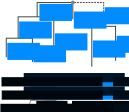
\includegraphics[width=1\linewidth]{pdf/balances.pdf}
    \begin{subfigure}{0pt}
        \phantomcaption
        \label{fig:balances:sub:masses}
    \end{subfigure}
    \begin{subfigure}{0pt}
        \phantomcaption
        \label{fig:balances:sub:tree}
    \end{subfigure}
    \begin{subfigure}{0pt}
        \phantomcaption
        \label{fig:balances:sub:calculation}
    \end{subfigure}
    \begin{subfigure}{0pt}
        \phantomcaption
        \label{fig:balances:sub:balances}
    \end{subfigure}
    \caption[Example computation of the balances between two subtrees]{
        \textbf{Example computation of the balances between two subtrees.}
        \subref{fig:balances:sub:masses}
        The basis of the computation are the per-branch masses of the samples, 
        which are here summarized in the mass matrix, c.\,f. \figref{fig:masses_imbalances:sub:Matrices}.
        \subref{fig:balances:sub:tree}
        We here show the computation of the balance for the two subtrees induced by the dashed edge of the tree,
        for one sample.
        Numbers next to edges are the accumulated per-edge placement masses of the sequences in the sample,
        that is, one row of the matrix.
        We call the left hand side of the tree R, and the right hand side S, as seen from the dashed edge.
        For simplicity, we do not use weighting here; that is, we assume $\bm{p} = ( 1, \ldots, 1 )$.
        \subref{fig:balances:sub:calculation}
        First, the geometric means for both subtrees are calculated, then, their balance.
        The balance is positive, indicating that subtree R contains more placement mass on (geometric) average.
        \subref{fig:balances:sub:balances}
        The compuation is repeated for all edges and for all samples, yielding the \emph{balance matrix} shown here.
    }
    \label{fig:balances}
\end{figure}

% balance can be computed for nodes, subtrees, or -- similar to imbalances, for two sides of an edge.
Balances as defined here can be computed as a measure of \emph{contrast} between any disjoint sets $R$ and $S$ of edges.
Interchanging $S$ and $R$ flips the sign of the balance;
this is irrelevant for the subsequent steps presented here, as long as the interchange is applied consistently.
% We decided for the convention of using the subtree that contains the root for the numerator,
% in accordance with edge imbalances.
When computing the balance between the edges in the two subtrees induced by some given edge $e$,
the conceptual similarity with the previously described edge imbalances 
(\secref{ch:Foundations:sec:PhylogeneticPlacement:sub:PlacementProcessing:par:EdgeImbalances}) becomes apparent:
Imbalances use the difference of sums for contrasting and aggregating,
while balances use the ratio of means for the same purpose.
Hence, balances represent a similar transformation of the placement data,
that can also be used to conduct analyses, such as the Phylofactorization, as presented in \chpref{ch:Factorization}.

We however remark that using (unweighted) balances in our previously presented methods,
such as Edge Correlation (\secref{ch:Visualization:sec:Methods:sub:EdgeCorrelation})
and $k$-means clustering (\secref{ch:Clustering:sec:Methods:sub:PhylogeneticKmeans}),
might lead to spurious results, due to the insensitivity of the geometric mean to singular large values.
That is, individual branches that accumulate a large fraction of the placement mass (sequence abundances)
might only insignificantly change the geometric mean of their clade.
However, such branches are typically the interesting ones,
and hence should exert more influence on the transformation, which is exactly the purpose of the taxon weighting scheme.
This further implies that balances are not indifferent to splittings of reference taxa into multiple representatives
(pers.~comm. with A.~Washburne on 2018-11-23).
%the distribution of placement masses across several branches of related species
% yields different balances compared to having a single representative taxa in the \ac{RT};
We discuss the implications of this in more detail in the evaluation of the method (\secref{ch:Balances:sec:Results}).

% Hence, balances can also be employed for our other methods presented above, such as
% \nameref{sec:MaterialsMethods:sub:Visualization:sub:Correlation} and
% \nameref{sec:MaterialsMethods:sub:Clustering:sub:kmeans}.

% Comparing the per-node balance across samples allows to find nodes that change with respect to the balance,
% indicating ``factors'' that explain differences between the samples in terms of the phylogeny.
% The transformation into balances yields orthogonal components, which are not compositional any more,
% and can hence be used with many standard analysis methods.

% ----------------------------------------------------------------------------------------------------------------------
%     Edge Weights
% ----------------------------------------------------------------------------------------------------------------------

\subsection{Taxon Weighting Scheme}
\label{ch:Balances:sec:Methods:sub:EdgeWeights}

The PhILR also allows for incorporating two distinct weighting schemes for the balances,
one based on taxon abundances, and one based on the branch lengths of the underlying phylogeny \cite{Silverman2017}.
As mentioned above, we implemented the former, while leaving the latter as future work.

We here describe how to adapt the taxon weights of \cite{Silverman2017} to our placement-based approach,
that is, how an appropriate vector $\bm{p}$ of edge weights can be constructed.
Originally, this taxon weighting scheme down-weighs the influence of low abundant taxa \cite{Silverman2017},
which are known to be less reliable and more variable \cite{Good1956}.
Here, we accordingly down weigh edges with low placement mass, for the same reasons.
We follow the approach of \cite{Silverman2017}, and construct the edge weights by multiplicatively combining two terms:

\begin{enumerate}
    \item A measure for the central tendency of the absolute edge masses, for example, their mean across all samples.
          This is the main component of the weight that yields low values for edges with low mass and vice versa.
    \item A vector norm of the relative edge masses across the samples.
          This term additionally weighs edges by their specificity.
\end{enumerate}

Our implementation allows to use the median, the arithmetic mean, and the geometric mean,
as well as different $\ell_p$-norms (such as the Manhattan, Euclidean, and maximum norm),
and the Aitchison norm \cite{Pawlowsky-Glahn2015}.
We follow the advice of \cite{Silverman2017}, and by default use the geometric mean
(with pseudo-counts added to the masses to avoid skew from edges without any placement mass) and the Euclidean norm.
In that case, the weights for edge $j$ are computed as follows:

\begin{equation}
    \label{ch:Balances:sec:Methods:eq:EdgeWeights}
%     p_j = \sqrt[n]{ ( c_{j1} + 1 ) \cdot \ldots \cdot ( c_{jn} + 1 ) } \cdot \| x_j \|
%     p_j ~=~ \sqrt[n]{ \prod_{i=1}^{n} ( \tilde{c}_{ji} + 1 ) }  ~\cdot~  \| \tilde{x}_j \|_2
    p_j ~=~ \sqrt[n]{ \prod_{i=1}^{n} ( \tilde{c}_{ji} + 1 ) }  ~~\cdot~  \sqrt{ \sum_{i=1}^{n} \tilde{x}_{ji}^2 }
\end{equation}

Here, $n$ is the number of samples, $\tilde{c}_j$ is the vector of absolute masses at edge $j$ across all samples,
and $\tilde{x}_j$ the vector of relative masses at edge $j$ across all samples, both of length $n$.
That is, these measures use the masses of all $n$ samples;
consequently, we here use columns instead of rows of the edge masses matrix of \figref{fig:masses_imbalances:sub:Matrices},
where each column is used for the weights of the corresponding edge.
The resulting edge weights $\bm{p}$ are then fixed and used across the balance computation of all samples.

% this corresponds to taxon weights of \cite{Silverman2017}.
% as we consider masses on edges instead of abundances at the tips of the tree, we use the term edge weights instead of taxon weights here.
% note that these weights are meant as a weighting mechanism to reduce the influence of low abundance taxa / edges with low mass.
% the terms weight and mass should not be confused here!

% ######################################################################################################################
%         Evaluation and Results
% ######################################################################################################################

\section{Evaluation and Results}
\label{ch:Balances:sec:Results}

As a first test of our adaptation of balances to placement data, we apply it to the \ac{BV} dataset \cite{Srinivasan2012}.
Further assessment of balances for placement data, also with the \ac{HMP} dataset \cite{Huttenhower2012,Methe2012},
is implicitly conducted by the evaluation of Placement-Factorization in \secref{ch:Factorization:sec:Evaluation},
which uses balances for aggregation and contrasting of subtrees.
% We hence refrain here from further tests.
See \appref{supp:sec:DetailsEmpiricalDatasets:sub:BV} and \appref{supp:sec:DetailsEmpiricalDatasets:sub:HMP}
for descriptions of the datasets.

% ----------------------------------------------------------------------------------------------------------------------
%     Principal Components
% ----------------------------------------------------------------------------------------------------------------------

\subsection{Principal Components}
\label{ch:Balances:sec:Results:sub:PrincipalComponents}

As balances are conceptually similar to edge imbalances, we perform analogous evaluations.
To this end, we computed the per-edge balance for all edges of the \ac{BV} reference tree, across all \num{220} samples.
That is, for each edge, we computed the balance between the two subtrees induced by the edge.
This yields a matrix that we call \emph{balance matrix}, as shown in \figref{fig:balances:sub:balances},
which corresponds to the imbalance matrix used for Edge PCA, c.\,f. \figref{fig:masses_imbalances:sub:Matrices}.
Hence, a natural first visualization of the balances is to analyze their principal components,
that is, to compute the PCA of the balance matrix.
The first two components of the \ac{BV} balances are shown in \figref{fig:bv_place_edge_balances_pca_scatter},
for both variants of the balance computation (with and without taxon weighting).
% The principal components exhibit a separation of the samples by Nugent score,
% showing that they yield results comparable to Edge PCA.
% In order to interpret what the axes of these principal components mean,
Furthermore,
we can again employ the visualization of PCA eigenvectors on the reference tree as used in Edge PCA \cite{Matsen2011a}.
% c.\,f., \figref{fig:epca}.
We show the results for %PCA on the balances of 
the \ac{BV} dataset in \figref{fig:bv_place_edge_balances_pca_trees},
where we visualize the first two principal components of the balances with and without taxon weighting on the tree.
% The figure shows the edges that are responsible for the splits seen in \figref{fig:bv_place_edge_balances_pca_scatter}.

\begin{figure}[!htb]
    \centering
    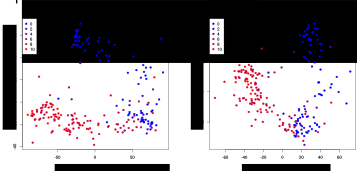
\includegraphics[width=\linewidth]{pdf/bv_place_edge_balances_pca_scatter.pdf}
    \begin{subfigure}{0pt}
        \phantomcaption
        \label{fig:bv_place_edge_balances_pca_scatter:sub:with_taxon_weighting}
    \end{subfigure}
    \begin{subfigure}{0pt}
        \phantomcaption
        \label{fig:bv_place_edge_balances_pca_scatter:sub:without_taxon_weighting}
    \end{subfigure}
    \caption[Projection of edge balance PCA components of the \acs{BV} dataset]{
        \textbf{Projection of edge balance PCA components of the \ac{BV} dataset.}
        The plots show the first two principal components of a PCA on the per-edge balances,
        calculated on placements of the data on reference tree of the \ac{BV} dataset.
        That is, for each edge of the tree, we calculated the balance (log-ratio of geometric means)
        of the placement masses of the \ac{BV} samples between the two sides of the tree induced by the edge.
        Then, we computed a PCA on the resulting balance matrix.
        \subref{fig:bv_place_edge_balances_pca_scatter:sub:with_taxon_weighting} shows the result when
        using taxon weighting \cite{Silverman2017} in the balances calculation,
        while \subref{fig:bv_place_edge_balances_pca_scatter:sub:without_taxon_weighting} shows the result
        without taxon weighting.
        Each item represents a sample, colored by its Nugent score (0 means healthy, 10 means severe illness);
        the Nugent score had no influence on the PCA calculations.
    }
    \label{fig:bv_place_edge_balances_pca_scatter}
\end{figure}

\begin{figure}[!phtb]
    \centering
    \includegraphics[width=\linewidth]{pdf/bv_place_edge_balances_pca_trees.pdf}
    \begin{subfigure}{0pt}
        \phantomcaption
        \label{fig:bv_place_edge_balances_pca_trees:sub:tw_pc1}
    \end{subfigure}
    \begin{subfigure}{0pt}
        \phantomcaption
        \label{fig:bv_place_edge_balances_pca_trees:sub:tw_pc2}
    \end{subfigure}
    \begin{subfigure}{0pt}
        \phantomcaption
        \label{fig:bv_place_edge_balances_pca_trees:sub:no_tw_pc1}
    \end{subfigure}
    \begin{subfigure}{0pt}
        \phantomcaption
        \label{fig:bv_place_edge_balances_pca_trees:sub:no_tw_pc2}
    \end{subfigure}
    \caption[Eigenvectors of edge balance PCA of the \acs{BV} dataset]{
        \textbf{Eigenvectors of edge balance PCA of the \ac{BV} dataset.}
        The figure shows the eigenvectors of the first two principal components of PCA
        on the per-edge balances with and without taxon weighting,
        visualized on the reference tree of the \ac{BV} dataset.
%         See \figref{fig:bv_place_edge_balances_pca_scatter} for details on the balances calculation.
        The visualization of the components on the reference tree is analogous
        to the Edge PCA tree visualization as for example shown in \figref{fig:epca}.
        As the data that is considered in the PCA corresponds to the edges of the tree,
        the resulting eigenvectors can be mapped back onto the tree, which is shown here.
        Each edge is colored according to the corresponding value of the first principal component
        in \subref{fig:bv_place_edge_balances_pca_trees:sub:tw_pc1}
        and \subref{fig:bv_place_edge_balances_pca_trees:sub:no_tw_pc1},
        and the second principal component
        in \subref{fig:bv_place_edge_balances_pca_trees:sub:tw_pc2}
        and \subref{fig:bv_place_edge_balances_pca_trees:sub:no_tw_pc2}, respectively.
        In \subref{fig:bv_place_edge_balances_pca_trees:sub:tw_pc1}
        and \subref{fig:bv_place_edge_balances_pca_trees:sub:no_tw_pc1},
        we marked the \taxonname{Lactobacillus crispatus} clade with a black arc at the left of the tree.
    }
    \label{fig:bv_place_edge_balances_pca_trees}
\end{figure}

\figref{fig:bv_place_edge_balances_pca_trees} hence indicates how the axes of the principal components
in the PCA scatter plots of \figref{fig:bv_place_edge_balances_pca_scatter} can be interpreted:
The first component leads to the \taxonname{Lactobacillus} clade,
while the second one splits this clade into \taxonname{Lactobacillus iners} and \taxonname{Lactobacillus crispatus}.
Both plots of \figref{fig:bv_place_edge_balances_pca_scatter} separate the healthy from the sick patients.
However, in contrast to Edge PCA, the first component of
\figref{fig:bv_place_edge_balances_pca_scatter:sub:with_taxon_weighting}
does not fully distinguish between the healthy (blue) and diseased (red) samples.
For yet to explore reasons, the component only takes \taxonname{Lactobacillus iners} into account,
while mostly ignoring \taxonname{Lactobacillus crispatus}.
This can be seen in \figref{fig:bv_place_edge_balances_pca_trees:sub:tw_pc1},
which shows the eigenvectors of this component visualized on the reference tree.
There, the path leading to the \taxonname{Lactobacillus} clade
does not include the branches of \taxonname{Lactobacillus crispatus}, which is marked with a black arc.
Including the second component however, which distinguishes between the two types of \taxonname{Lactobacillus},
as shown in \figref{fig:bv_place_edge_balances_pca_trees:sub:tw_pc2},
yields a clear separation of the samples.
On the other hand, \figref{fig:bv_place_edge_balances_pca_scatter:sub:without_taxon_weighting}
exhibits closer similarities to the Edge PCA plot shown in \figref{fig:kmeans_all:sub:epca_ns},
in that the first component separates healthy from sick,
and the second component further splits the healthy individuals apart.
% In fact, the only difference to Edge PCA is the use of balances instead of imbalances for the PCA.

Hence, the results obtained from this analysis are consistent with our previous findings, in particular with Edge PCA.
% c.\,f., \figref{fig:epca} and \cite{Srinivasan2012}.
% in order to show that balances without taxon weighting do not include this clade in the first component.
The principal components separate the samples by Nugent score,
with the first component mostly separating \taxonname{Lactobacillus} from the rest of the tree,
and the second component further distinguishing
between \taxonname{Lactobacillus crispatus} and \taxonname{Lactobacillus iners}.

% showing that they yield results comparable to Edge PCA.
% As with Edge PCA, the principal components correspond to the \taxonname{Lactobacillus} clade,

% ----------------------------------------------------------------------------------------------------------------------
%     Edge Correlation
% ----------------------------------------------------------------------------------------------------------------------

\subsection{Edge Correlation}
\label{ch:Balances:sec:Results:sub:EdgeCorrelation}

As mentioned in the method description (\secref{ch:Balances:sec:Methods:sub:ILRTransform}),
balances could in principle be used as input to our previously presented methods,
such as Edge Correlation and $k$-means clustering (which adequately might be called Balance $k$-means),
in the same manner that we used imbalances in these methods.
To provide an example of using balances with these methods, 
we show the correlation of the Nugent score with balances in \figref{fig:bv_place_edge_balances_correlation}.

\begin{figure}[!htb]
    \centering
    \includegraphics[width=\linewidth]{pdf/bv_place_edge_balances_correlation.pdf}
    \begin{subfigure}{0pt}
        \phantomcaption
        \label{fig:bv_place_edge_balances_correlation:sub:with_taxon_weighting}
    \end{subfigure}
    \begin{subfigure}{0pt}
        \phantomcaption
        \label{fig:bv_place_edge_balances_correlation:sub:without_taxon_weighting}
    \end{subfigure}
    \caption[Correlation of the edge balances of the \acs{BV} dataset with Nugent score]{
        \textbf{Correlation of the edge balances of the \ac{BV} dataset with Nugent score.}
        The Edge Correlation method as presented in \secref{ch:Visualization:sec:Methods:sub:EdgeCorrelation},
        and for example shown in \figref{fig:all_nugent},
        can also be conducted using balances (instead of masses or imbalances).
        We here show Edge Correlation using Spearman's Rank Correlation Coefficient,
        calculated on the per-edge balances and the Nugent score, based on the placement of the \ac{BV} dataset.
        That is, for each edge of the tree, we calculated the balance (log-ratio of geometric means)
        of the placement masses of the \ac{BV} samples between the two sides of the tree induced by the edge.
        Then, we calculated the correlation with the Nugent score of each sample, and visualized it on the tree.
        \subref{fig:bv_place_edge_balances_correlation:sub:with_taxon_weighting} shows the result when
        using taxon weighting \cite{Silverman2017} in the balances calculation,
        while \subref{fig:bv_place_edge_balances_correlation:sub:without_taxon_weighting} shows the result
        without taxon weighting.
    }
    \label{fig:bv_place_edge_balances_correlation}
\end{figure}

The result of this balance-based Edge Correlation with taxon weighting,
shown in \figref{fig:bv_place_edge_balances_correlation:sub:with_taxon_weighting},
is similar to the correlation with imbalances in \figref{fig:all_nugent:sub:srcc_ei}:
An anti-correlation with the \taxonname{Lactobacillus} clade is again visible
(less placement mass in this clade means higher Nugent score, that is, indicates a more severe illness),
while several other clades exhibit a positive correlation with Nugent score.
Hence, balance-based Edge Correlation \emph{with} taxon weighting is consistent with our previous findings,
and with the imbalance-based variant of this method.

However, artifacts might arise from the underlying mathematical framework of balances,
in particular the usage of the geometric mean \emph{without} taxon weighting:
The geometric mean is \emph{not} sensitive to singular large values,
such as the high amount of placement mass on one of the \taxonname{Lactobacillus} branches.
It only significantly increases if multiple high values are present,
such as the multitude of bacterial taxa with high abundance in diseased patients of the \ac{BV} dataset \cite{Srinivasan2012}.
This can lead to spurious results, as shown in
\figref{fig:bv_place_edge_balances_correlation:sub:without_taxon_weighting},
where the correlation of the unweighted balances %without taxon weighting
with the Nugent score yields unrealistically high negative correlations
for almost all branches that have little placement mass on them (red branches).

%         However, as mentioned in the main text, without taxon weighting, spurious results can occur.
% The most striking difference to the previous Edge Correlation trees in \figref{fig:all_nugent}
% is however the majority of spuriously anti-correlated (red) edges in the tree \emph{without} taxon weighting
% in \figref{fig:bv_place_edge_balances_correlation:sub:without_taxon_weighting}.
% As mentioned in the method description in \secref, this is due to the insensitivity of the geometric mean
% to the presence of singular large values:
The reason that the insensitivity of the geometric mean to the presence of singular large values
leads to the majority of spuriously anti-correlated edges is as follows:
If most values are small, so will be their geometric mean, even if a few very large values are also present.
As can be seen in \figref{fig:heat_tree} and \figref{fig:all_dispersions},
the clades that exhibit a high anti-correlation here (red) have low placement mass with a low variance.
Hence, the geometric mean of the masses in these clades is consistently low across samples,
which means that the numerator of the log-ratio in the balances computation has little effect on the correlation.
This implies that the denominator, which represents the rest of the tree, drives the anti-correlations seen here.
Women affected by \ac{BV} show a presence of several different bacterial clades,
while healthy women without \ac{BV} almost exclusively have high presence
of one of two types of \taxonname{Lactobacillus} \cite{Srinivasan2012}.
Hence, in samples with \ac{BV} (high Nugent score), there are several distinct edges that have an elevated mass,
which is enough to change the geometric mean,
while in samples without \ac{BV} (low Nugent score),
most of the mass is concentrated on a single edge of the \taxonname{Lactobacillus} clade,
which is not enough to significantly change the geometric mean.
In consequence, the denominator of the balance at the spurious edges is consistently larger
for samples with \ac{BV} compared to those without \ac{BV}.
Thus, the balance is smaller for samples with a high Nugent score,
which finally explains the observed anti-correlations.
Note that despite this, there are still edges that exhibit positive correlation (blue and green),
which is where the actual patterns in the data outweigh the insensitivity of the geometric mean.

Lastly, this property of insensitivity of the geometric mean implies that it \emph{is} sensitive to taxa splitting,
that is, to the number of reference sequences that a taxon or species is represented by in the reference tree
(pers.~comm. with A.~Washburne on 2018-11-23):
For example, in the context of balances of phylogenetic placements,
it \emph{does} make a difference whether masses are focused on a single branch,
or distributed across several representatives of the same species.
Hence, in summary,
we do not recommend to use (unweighted) balances for computations such as correlations or $k$-means clustering.

% ######################################################################################################################
%         Summary and Outlook
% ######################################################################################################################

\section{Summary and Outlook}
\label{ch:Balances:sec:SummaryOutlook}

In this chapter, we introduced an adaptation of the Phylogenetic ILR transform and balances \cite{Silverman2017}
to phylogenetic placements.
Balances are conceptually similar to edge imbalances, exhibit similar properties, 
and can be used for similar types of analyses.
% hence combining previously existing concepts from different 
% of OTU-based balances with placement-based edge imbalances.
Hence, with this adaptation, we helped to bridge the methodological gap 
between OTU-based and placement-based approaches to analysing metagenomic data.
This might lead to future development of novel methods and adaptations,
with the intention of obtaining a better, more complete picture of metagenomic data,
by combining the strengths of both the OTU-based and the placement-based approaches.

As balances are a transformation that yields orthogonal components (one for each node or branch of the tree),
issues pertaining to the normalization of compositional data do not arise.
With samples being represented as a vector of balances,
numerous standard tools for data visualization, ordination, and clustering in the euclidean space
can be readily applied to phylogenetic placement data.
Applying these methods to placements instead of OTUs allows for more detailed analyses,
as the entire original sequence data can be used.
Furthermore, using a fixed reference tree instead of one inferred from the OTUs present in a set of samples
enables comparative studies across datasets.

In the context of this work, balances are used as an intermediary tool
in order to describe a set of samples in the context of a reference tree.
In this chapter, we evaluated some basic analysis and visualization techniques in order to show
that balances yield consistent results on empirical data sets compared to concepts such as edge imbalances.
In the following chapter, we introduce Placement-Factorization,
which uses balances as a description of clades of the reference tree.

% ######################################################################################################################
%         Placement-Factorization
% ######################################################################################################################

\chapter{Placement-Factorization}
\label{ch:Factorization}

\paperbox{
    This chapter is based on the peer-reviewed publication:
}{\paperpppp}{
    \textbf{Contributions:} Lucas Czech... Alexandros Stamatakis...
    \todo{}
}

% \todo{distance measures, nhd, simulations, mantel test}

% ######################################################################################################################
%         Background and Motivation
% ######################################################################################################################

\section{Background and Motivation}
\label{ch:Factorization:sec:Motivation}

Phylofactorization is a method to identify edges in a phylogenetic tree
that drive patterns in the composition of microbial communities \cite{Washburne2017a}.
An edge constitutes a separation or split of groups of taxa into the two subtrees induced by the edge.
In an evolutionary context, an edge denotes a difference in (putative) traits that may have arisen along the edge.
That is, an edge might describe characteristics and traits
that are only present in the set of taxa on one side of the edge, but not in the set on the other side.
The goal of Phylofactorization is to identify edges that are related to differences in per-sample meta-data features.
% That is, it finds groups of taxa for which a change in abundances is reflected in changes in environmental variables.
To this end, it aggregates and contrasts the abundances in the subtrees (groups of taxa) induced by an edge,
and evaluates how changes in environmental variables across samples are reflected in abundance changes.

The original method \cite{Washburne2017a} uses a tree inferred from the OTUs that are present in the set of samples,
% and represents each sample by its OTU abundances at the tips of the tree.
% Each edge splits the tree, and thus induces clades that correspond to sets of OTUs,
% which are called \emph{binned phylogenetic units} (BPUs) in this context.
and iteratively identifies edges that split the tree into nested subtrees
which exhibit the largest predictable differences between the taxa in these subtrees.
Each such edge can be interpreted as a \emph{phylogenetic factor} (or short, \emph{phylofactor}) for splitting the tree:
Once an edge has been selected in one iteration, its induced subtrees are then considered separately in subsequent iterations.
The resulting factors are hence independent of each other, which ensures orthogonality of the factors.
In other words, each factor describes a different dimension in which samples differ. %, analogous to Edge PCA.
Furthermore, by iteratively considering subtrees of decreasing size, nested factors can be found,
which correspond to relationships within a subtree that only affect the taxa in the subtree itself.
The algorithm stops after a predefined number of iterations/factors, %(that is, until a certain number of edges have been found),
or until a stopping criterion is met.

In a typical use case, each environmental sample is represented by its OTU abundances at the tips of the tree,
that is, by counts of how often each OTU is present in the sample; 
see \secref{ch:Foundations:sec:SequenceAnalysis:sub:OTUs} for details on OTUs of metagenomic samples.
Given a per-sample meta-data feature such as the pH-value,
Phylofactorization can then be employed to find edges where a change of the pH-value between samples
predicts a change in OTU abundances in the two subtrees induced by the edge.
For example, an increasing ph-value might indicate
a relative increase in the OTU abundances in one subtree compared to another subtree.
The resulting factorization can serve as a dimensionality-reduction mechanism, as an ordination and visualization tool,
and as an inferential tool that can identify edges corresponding to changes in functional ecological traits \cite{Washburne2017a}.
We later showcase some of these applications in \secref{ch:Factorization:sec:Evaluation}.

% ######################################################################################################################
%         Methods and Implementation
% ######################################################################################################################

\section{Methods and Implementation}
\label{ch:Factorization:sec:Methods}

We here present an adaptation of Phylofactorization to phylogenetic placements, which we call \emph{Placement-Factorization}.
We explain our adaptation following the description of the Generalized Phylogenetic Factorization (GPF) \cite{Washburne2018,Washburne2019}.
The GPF is a recent generalization of Phylofactorization
that also allows for types of input data other than relative OTU abundances, for example, presence/absence data.
It is hence suited for a wider range of community ecological data \cite{Washburne2019}.
Conceptually and algorithmically, Phylofactorization, GPF, and our Placement-Factorization, work the same;
we here use the mathematical notation of GPF as a scaffold to explain our adaptation.
In the following, we briefly introduce the original method, outline the necessary adaptations,
and explain how to use the balances obtained from (our adaptation of)
the PhILR transform (as explained in \chpref{ch:Balances}) in the context of Placement-Factorization.

% ======================================================================================================================
%     Placement Factorization
% ======================================================================================================================

\subsection{Placement-Factorization}
\label{ch:Factorization:sec:Methods:sub:Phylofactor}

Phylofactorization can be understood as an iterative greedy graph-partitioning algorithm for a tree $T$ \cite{Washburne2018}.
In each iteration, a \emph{winning edge} $e^*$ is identified
that splits edges of the tree into two disjoint groups $R$ and $S$.
To determine the winning edge, an \emph{objective function} is maximized
that expresses the intensity of the relationship between abundances and meta-data variables.
We later discuss this objective function in more detail in \secref{ch:Factorization:sec:Methods:sub:ObjectiveFunction}.

% ------------------------------------------------
%     Input
% ------------------------------------------------

\paragraph{Input}
\label{ch:Factorization:sec:Methods:sub:Phylofactor:par:Input}

The input to the original Phylofactorization is an $n \times m$ data matrix $X$,
containing $j = 1, \ldots, n$ samples, and $i = 1, \ldots, m$ species (corresponding to the OTUs at the tips of the tree).
The values of the matrix can represent abundances, presence/absence data, 
or other data related to the species in the tree \cite{Washburne2019}.

In our adaptation, we use the per-edge masses from the phylogenetic placement of the samples.
% (disregarding that the matrix is transposed here compared to the notation used there).
That is, instead of $m$ species representing the tips of the tree,
we use an $n \times m$ data matrix $X$ where the $m$ columns correspond to the edges of our reference tree
(for consistency of notation, we re-use and re-purpose the index $m$ here,
and transpose $X$ compared to the original notation).
This is again the mass matrix that we used in the previous methods (\chpref{ch:Visualization} and \chpref{ch:Clustering}),
and which we showed before in \figref{fig:masses_imbalances:sub:Matrices} and \figref{fig:balances:sub:masses}.

Lastly, Phylofactorization uses an $n \times p$ meta-data matrix $Z$ for the $n$ samples
and $p$ per-sample meta-data variables.
This is the same meta-data matrix that we used for example in Edge Correlation
(\secref{ch:Visualization:sec:Methods:sub:EdgeCorrelation}) and showed in \figref{fig:masses_imbalances:sub:Matrices}.

% ------------------------------------------------
%     Algorithm
% ------------------------------------------------

\paragraph{Algorithm}
\label{ch:Factorization:sec:Methods:sub:Phylofactor:par:Algorithm}

In analogy to the Generalized Phylofactorization \cite{Washburne2018,Washburne2019},
our adapted algorithm requires three functions:

\begin{enumerate}
    \item An \emph{aggregation function} $A_R = A( X_{j,R}, ~T )$,
          which aggregates (summarizes) a subset $R$ of edges for a sample $j$.
    \item A \emph{contrast function} $C_{R,S} = C( A_R, ~A_S, ~T, ~e )$, which contrasts (compares)
          the aggregates of two disjoint subsets $R$ and $S$ of edges on the two sides induced by an edge $e$.
          % C( A( X_{j,R}, T ), A( x_{j,S}, T ), T, e )
    \item An \emph{objective function} $\omega(C, ~Z)$ that evaluates a contrast for all samples
%          (for example, the contrast between groups $R$ and $S$ induced by a given edge)
          in the context of the per-sample meta-data, in order to determine the winning edge.
\end{enumerate}

We later discuss appropriate choices for these functions.
For now, we assume that we are given functions that allow identifying edges
whose induced subtrees exhibit predictable differences in the edge masses $X$
driven by changes in the meta-data $Z$ of different samples.
The algorithm starts by considering the entire tree $T$ as one large ``subtree''.
Then, in each iteration, Phylofactorization and Placement-Factorization work as follows:

\begin{enumerate}
    \item For each edge $e$ that separates disjoint groups $R_e$ and $S_e$ of edges within the subtree that contains $e$:
          \begin{enumerate}
              \item Compute the aggregates $A_{R_e} = A( X_{j,R_e}, ~T )$ and $A_{S_e} = A( X_{j,S_e}, ~T )$.
              \item Compute their contrast $C_e = C( A_{R_e}, ~A_{S_e}, ~T, ~e )$. %$C_{R_e, S_e}$.
              \item Compute the objective value $\omega_e = \omega(C_e, ~Z)$.
          \end{enumerate}
          The aggregates $A_{R_e}$ and $A_{S_e}$, as well as the contrast $C_e$ are computed separately for every sample.
          The value $\omega_e$ of the objective function then expresses the relationship of the contrasts of all samples
          with their respective meta-data values in $Z$.
    \item Select the winning edge $e^* = \argmax_e ( \omega_e )$ that maximizes the value of the objective function.
    \item Partition the subtree that contains the winning edge $e^*$ into two disjoint subtrees, separated by $e^*$.
    \item Repeat until a stopping criterion is met.
\end{enumerate}

This closely follows the description of the algorithm in \cite{Washburne2018,Washburne2019}, see there for details.
The difference between the algorithms is that the groups $R$ and $S$ in our case consist of reference tree edges,
instead of species at the tips of the OTU tree.
Because of this, the aggregates of edges that lead to tip nodes are empty,
meaning that we do not consider those edges as candidates in the algorithm.
This is analogous to ``tip edges'' not having a meaningful edge imbalance, 
as described in \secref{ch:Foundations:sec:PhylogeneticPlacement:sub:PlacementProcessing:par:EdgeImbalances}.
An example of the first two iterations of the algorithm is shown in \figref{fig:phylofactor}.

\begin{figure}[!htbp]
    \centering
    \includegraphics[width=\linewidth]{pdf/phylofactor.pdf}
    \begin{subfigure}{0pt}
        \phantomcaption
        \label{fig:phylofactor:sub:heat_tree}
    \end{subfigure}
    \begin{subfigure}{0pt}
        \phantomcaption
        \label{fig:phylofactor:sub:first}
    \end{subfigure}
    \begin{subfigure}{0pt}
        \phantomcaption
        \label{fig:phylofactor:sub:second}
    \end{subfigure}
    \caption[Input data and first two iterations of Placement-Factorization]{
        \textbf{Input data and first two iterations of Placement-Factorization.}
        The figure resembles Figure~2 of \citeay{Washburne2017a}.
        It shows the adaptation of concepts from Phylofactorization to phylogenetic placement data.
        \\
        \subref{fig:phylofactor:sub:heat_tree}
        The input data is a set of samples with placement masses on each edge of the tree.
        The tree is colorized by the total mass across all samples, that is, by the row sums of the heat map.
        The heat map then shows the detailed mass per edge (rows) and per sample (columns),
        and hence is an example of the mass matrix of \figref{fig:masses_imbalances:sub:Matrices}.
        Note that the heat map also contains rows for each inner edge of the tree,
        as phylogenetic placement also considers these edges.
        This is different from OTU abundance heat maps that only have entries for the tips of the tree.
        We show a further example of this visualization for empirical data in \figref{fig:heat_tree}.
        \\
        \subref{fig:phylofactor:sub:first} In the first iteration,
        the objective function for all inner edges is evaluated.
        Here, edge $e_1$ is the winning edge that maximizes the objective function,
        which separates the clade ({\sffamily A}, {\sffamily B}, {\sffamily C}, {\sffamily D}) from the rest of the tree.
        \\
        \subref{fig:phylofactor:sub:second} In the second iteration,
        only the contrasts within the two subtrees %(orange and black)
        are calculated,
        but not across the winning edges of previous iterations (here, $e_1$).
        That is, the winning edge $e_2$ maximizes the objective function that contrasts clade ({\sffamily F}, {\sffamily G})
        with clade ({\sffamily E}, {\sffamily H}, {\sffamily I}),
        but does not consider the edges in the subtree ({\sffamily A}, {\sffamily B}, {\sffamily C}, {\sffamily D}).
        Note that in our adaption, edges that lead to a tree tip are not considered as potential factors.
    }
    \label{fig:phylofactor}
\end{figure}

Each iteration further splits a subtree at the respective winning edge,
so that after $i$ iterations, $i+1$ subtrees are produced.
It is important to note that the winning edges of previous iterations split the tree into \emph{disjoint} subtrees,
and that in later iterations,
the aggregates and contrasts induced by an edge are only computed \emph{within} their respective subtrees.
This ensures the previously mentioned orthogonality of the phylogenetic factors (winning edges),
meaning that systematic dependencies between the contrasts of any two factors are eliminated,
and that instead, nested relationships can be identified.

The original publication proposes a stopping criterion using a Kolmogorov-Smirnov (KS) test \cite{Massey1951}
based on % (significance levels of)
test statistics of the identified phylofactors \cite{Washburne2017a,Washburne2019}.
Although these could be implemented for Placement-Factorization, we leave this as future work;
our implementation currently runs for a given number $i$ of iterations, and hence computes $i$ phylofactors.
% We leave elaborate stopping criteria as future work.
% based on a Kolmogorov-Smirnov (KS) test of the distribution of P-values from analyses of variance of the regressions on candidate ILR coordinates.

So far, we have assumed to be given the three functions required for Phylofactorization.
The choice of these functions depends on the data $X$, the data $Z$, and the research question at hand.
In order to be consistent and comparable with the original implementation \cite{Washburne2017a},
in our evaluation we used the same set of functions,
namely the balances of the ILR transformation as explained in \chpref{ch:Balances} for aggregating and contrasting subtrees,
and an objective function based on \acfp{GLM}, 
which we explain in the following, 
see \secref{ch:Factorization:sec:Methods:sub:ObjectiveFunction} and \secref{ch:Factorization:sec:Methods:sub:GLMs}.

% ------------------------------------------------
%     Output
% ------------------------------------------------

\paragraph{Output}
\label{ch:Factorization:sec:Methods:sub:Phylofactor:par:Output}

The main output of the algorithm is the list of winning edges, that is, 
of the phylogenetic factors that have been identified.
% These can for example be visualized directly as coloured clades on the tree.
Furthermore, one can store detailled tables with the balances per sample for all factors,
the values of the objective function at each edge for all factors,
as well as much more intermediary data of the algorithm.
We later show examples of how these outputs can be used for analysis and visualization purposes
in \secref{ch:Factorization:sec:Evaluation}.

% Not relevant any more:
% For our adaptation, %of Phylofactorization to phylogenetic placement data,
% a straight-forward choice could for instance be the following:
% To aggregate a group of edges, their per-edge placement mass is summed up;
% to contrast two aggregates, their difference is taken;
% to evaluate a contrast (objective function), the correlation with per-sample meta-data is calculated.
% This choice of functions would basically be identical to using \nameref{sec:Introduction:sub:Imbalances}
% and \nameref{sec:MaterialsMethods:sub:Visualization:sub:Correlation} constrained to the subtrees of the factors,
% and would yield phylofactors that are consistent with these approaches.
% % \todo{should we also eval this? probably yes... will see if there is time.}
% % \todo{this might have downsides that should be explored fist, and we should test it, etc...
% % but at least mention that this is not the best choice, and why GLMs are better}
% However, in order to be consistent and comparable with the original implementation \cite{Washburne2017a},
% in our evaluation we used the same set of functions,
% namely the balances of the ILR transformation as explained above for aggregating and contrasting subtrees,
% and an objective function based on \acfp{GLM}, which we explain in the following.
% % In the following,

% Back from when the order of sections was different:
% In the following sections, we describe alternative choices for these functions,
% based on the suggestions of \cite{Silverman2017} and \cite{Washburne2017a}:
% First, we introduce the ILR Transform and balances, which can be used for aggregation and contrasting.
% We further consider a weighting scheme for taxa/edges with low abundance/mass.
% We then discuss the choice of the objective function in more detail,
% and explain how Generalized Linear Models can be employed to this end.
% In each section, we also explain the changes that are necessary
% in order to adapt these approaches to phylogenetic placements.
% Finally, we bring these concepts together by explaining how to use them
% for Phylofactorization in the context of phylogenetic placement.
% and elaborate on their advantages compared to other choices of functions.

% ======================================================================================================================
%     Objective Function
% ======================================================================================================================

\subsection{Objective Function}
\label{ch:Factorization:sec:Methods:sub:ObjectiveFunction}

% Phylofactorization requires an objective function $\omega(C, ~Z)$ that selects the winning edge $e^*$ of each iteration
% based on (i) the contrasts $C$ between the two subtrees induced by all edges, and (b) the meta-data variables in $Z$.
% The choice of objective function depends on the research question at hand;
% see \cite{Washburne2017a} and \cite{Washburne2018} for a thorough discussion.
% Typically, an appropriate objective function quantifies some form of relationship between $C$ and $Z$,
% for example, the variation in $C$ explained by regression on $Z$, or some other measure of correlation between the two.

Phylofactorization requires an objective function $\omega(C_e, ~Z)$
that quantifies the relationship between $C_e$ and $Z$ for a given edge $e$,
where $C_e$ are the contrasts between the two subtrees induced by $e$ for all samples (for example, the balances),
and $Z$ are the per-sample meta-data variables.
That is, both $C_e$ and $Z$ have size $n$, the number of samples,
with $Z$ potentially containing multiple columns (one for each meta-data feature).
In order to identify the winning edge $e^*$ of an iteration (the \emph{phylofactor}),
the function is evaluated for all edges, and the edge maximizing $\omega$ is selected.
The choice of the objective function depends on the research question at hand;
see \citeay{Washburne2017a} and \citeay{Washburne2018} for a thorough discussion.

Our implementation is as general as the original Phylofactorization \cite{Washburne2017a},
in that it allows for an arbitrary objective function.
For simplicity, and in line with the original publication,
we here focus on functions that treat the meta-data variables $Z$ as independent variables
and the contrasts $C_e$ as dependent variables whose relationship with $Z$ is assessed, for instance, via a predictive model.
Then, the selected phylogenetic factors correspond to edges
where a change in $Z$ most strongly predicts a change in $C_e$ across the samples,
that is, where the effect of the (independent) meta-data variables
on the (dependent) underlying data (e.g., per-clade abundances) is most pronounced.
We show an example in \figref{fig:balance_factors}.

\begin{figure}[!htbp]
    \centering
    \includegraphics[width=\linewidth]{pdf/balance_factors.pdf}
    \begin{subfigure}{0pt}
        \phantomcaption
        \label{fig:balance_factors:sub:bad}
    \end{subfigure}
    \begin{subfigure}{0pt}
        \phantomcaption
        \label{fig:balance_factors:sub:good}
    \end{subfigure}
    \caption[Examples of relationships between independent and dependent variables]{
        \textbf{Examples of relationships between independent and dependent variables.}
        The figure shows simulated examples of the relationship between the latitude
        where some (hypothetical) oceanic samples were taken from
        and the balance of two edges of a reference tree for these samples.
        In \subref{fig:balance_factors:sub:bad}, there is no apparent relationship
        between the balances at this edge and the latitudes.
        This means that the clades of the tree that are split by the edge do not separate samples by latitude,
        and hence contain species whose abundances are not affected by latidute.
%         that are formed by the corresponding edge across which the balance was calculated
        In \subref{fig:balance_factors:sub:good} on the other hand, the balance of each sample
        exhibits a strong linear relationship with its latidute.
        This indicates that the corresponding edge across which the balance was calculated
        is a good candidate for a factor.
    }
    \label{fig:balance_factors}
\end{figure}

% A simple starting point is to use the magnitude of correlation between $C_e$ and $Z$ as objective function.
% This is easy to compute and yields phylofactors that are consistent with our previously described in
% \nameref{sec:MaterialsMethods:sub:Visualization:sub:Correlation},
% and can reveal correlations at deeper, nested levels of the underlying tree.
% \todo{maybe refer to results/supplement for this, if we make any of this.}
% This however only allows for a single column (one meta-data feature) in $Z$,
% and does not work well with balances, as we show in our evaluation
% \todo{rephrase: and entails certain issues}
% \todo{maybe remove this part}.
% Furthermore, because the magnitude of the correlation has to be used
% in order for the maximization of the objective function to work,
% the direction of the correlation is lost.

% ------------------------------------------------
%     Generalized Linear Models
% ------------------------------------------------

\paragraph{Generalized Linear Models}
\label{ch:Factorization:sec:Methods:sub:ObjectiveFunction:par:GLMs}

A powerful approach is to model the relationship between $C_e$ and $Z$ via linear regression,
that is, we assess how well $Z$ can predict $C_e$.
In the simple one-dimensional case, this can be thought of as fitting a line through a scatter plot
of the meta-data feature on the $x$-axis and the contrasts on the $y$-axis, where each point represents one sample,
c.\,f. \figref{fig:balance_factors}.
This concept is generalized via the \acf{GLM} \cite{Nelder1972,McCullagh1989,Agresti2018}.
% We here provide a brief intuition about \acp{GLM}; for details see \cite{McCullagh1989} and \cite{Agresti2018}.
% We provide a brief introduction to \acp{GLM} in S3~Text; for details see \cite{McCullagh1989} and \cite{Agresti2018}.
% \todo{Will have to see whether I can finish this in time. If not, remove the above. The explanation here should be enough for now.}

We introduce \acp{GLM} in more detail in \secref{ch:Factorization:sec:Methods:sub:GLMs}.
In short, \acp{GLM} allow to predict a single (response) variable using multiple input (explanatory) variables.
Typically, the response variable is assumed to follow any distribution from the exponential family
(normal, exponential, Poisson, Binomial, etc.), which is given for balances as used here.
In contrast to this, the explanatory variables (the meta-data features)
are assumed to have a linear relationship with the response.
%, while the explanatory variables are assumed to be linear --> but transformation allows to use any input really.
Note that this mathematical restriction of the model does not mean
that only meta-data features can be used that behave linearly;
transformations and interactions of the features basically allow for arbitrary types of data.
For example, categorical variables such as the body site where a sample was taken from can be transformed
into so-called dummy variables that fulfill the requirements.
% We later use this for the \ac{HMP} dataset, see \secref{sec:Results:sub:Phylofactor:sub:HMPDataset}.

Once the model parameters of the \ac{GLM} have been estimated,
that is, once it has been fit to the data via some optimization algorithm,
% The most commonly used is the iteratively reweighted least squares (IRLS) method \cite{Burrus2012},
% which yields a maximum likelihood estimation of the model parameters, and which is what we use in our implementation.
we need to evaluate the \ac{GLM} for the purposes of Phylofactorization.
We are interested in a value for $\omega$ that expresses how well the meta-data variables explain the balances.
To this end, Phylofactorization and our adaptation thereof use the difference between the null deviance of the balances
and the deviance obtained from the \ac{GLM}.
% The null deviance can be understood as the deviation from the mean value of the balances.
This difference %between null deviance and deviance of the model
expresses how much better the model explains the balances than just predicting them from their mean.
For details on the usage of \acp{GLM} for Phylofactorization, see \cite{Washburne2017a}.

% In S3~Text, we also describe %how to assess how well a \ac{GLM} fits/predicts the data,
% how to evaluate a \ac{GLM} for our purposes here, that is, how to use it to obtain a value for $\omega$.

% ------------------------------------------------
%     Usage in Phylofactorization
% ------------------------------------------------

\paragraph{Usage in Phylofactorization}
\label{ch:Factorization:sec:Methods:sub:ObjectiveFunction:par:Usage}

Predictive models such as the \ac{GLM} expect the response variable (that is, the predicted values; here, the contrasts)
to have certain statistical properties.
In particular, linear models assume the deviation of response from the predicted value to be normally distributed.
The ILR transform for compositional data has been proven to behave asymptotically normal \cite{Egozcue2003,Pawlowsky-Glahn2011a},
which allows their application within standard multivariate methods,
and within \acp{GLM} as presented here.
% and to Phylofactorization and Placement-Factorization as presented here.

Lastly, we note that depending on the research question, other objective functions can be used,
see \cite{Washburne2017a,Washburne2018} for some examples.
For instance, simple test statistics such as the variation in $C_e$ explained by regression on $Z$ can be used.
Furthermore, instead of predicting contrasts from meta-data, one could be interested in the opposite,
that is, predicting a meta-data variable given the per-sample contrasts.
In this case, the maximization of the objective function yields edges that best predict a certain feature of the data;
this is suitable for identifying clades that can serve as a bio-indicator.
Using \acp{GLM} for this allows to model any type of meta-data variable;
for example, the binary information encoded in presence/absence data can be predicted using logistic regression.
While our implementation supports all those use cases,
they have been explored and discussed before \cite{Washburne2017a,Washburne2019}.
For the sake of simplicity, we focus on linear (gaussian) modeling of $C_e \sim Z$,
that is, predicting balances from meta-data.

% ======================================================================================================================
%     Generalized Linear Models
% ======================================================================================================================

\subsection{Generalized Linear Models}
\label{ch:Factorization:sec:Methods:sub:GLMs}

% Sources:
% https://en.wikipedia.org/wiki/Generalized_linear_model
% https://newonlinecourses.science.psu.edu/stat504/node/216/
% http://www.stat.cmu.edu/~ryantibs/advmethods/notes/glm.pdf
%
% https://www.sagepub.com/sites/default/files/upm-binaries/21121_Chapter_15.pdf
% https://bookdown.org/egarpor/SSS2-UC3M/logreg-deviance.html
% https://www.stat.berkeley.edu/~blfang/STAT151A/STAT151A_lab11.html

We now take a short digression to introduce the \acf{GLM} \cite{Nelder1972,McCullagh1989};
% This concept is generalized even further by a \acf{GLM} \cite{Nelder1972,McCullagh1989}.
% We provide a brief intuition about \acp{GLM} for the interested reader;
for a more detailled explanation see \citeay{McCullagh1989} and \citeay{Agresti2018}.
Note that the abbriviation GLM is sometimes also used for the \emph{general linear model},
as opposed to the \emph{generalized} linear model that we discuss here, which are distinct concepts.
Hence, sometimes, the latter is abbriviated as GLIM instead \cite{McCullagh1989}.
The \ac{GLM} is a generalization of linear regression that allows
% \acp{GLM} generalize from linear regression by allowing
(a) for the response variable to have an arbitrary error distribution model
(instead of a normal distribution, which is implicitly assumed in linear regression),
and (b) for an arbitrary function of the response variable---called the \emph{link function}---%
to vary linearly with the predicted values (instead of the response variable itself varying linearly).
In the context of the \ac{GLM},
the independent variables (e.\,g., $Z$) are called the \emph{predictor variables} or \emph{explanatory variables},
while the dependent variable (e.\,g., $C_e$) is called the \emph{response variable}.
The goal is then to best predict the (single) response variable from the (multiple) explanatory variables.

%  by allowing the magnitude of the variance of each measurement to be a function of its predicted value
% we here briefly describe the gaussian 1d case in order to provide some intuition about linear models
% here, we describe the simple linear case of using metadata to predict contrasts (which can for example be balances, as described above)
% The \ac{GLM} is a generalization of linear regression
% that allows for response variables that have error distribution models other than a normal distribution.

% ------------------------------------------------
%     Model Components
% ------------------------------------------------

\paragraph{Model Components}
\label{ch:Factorization:sec:Methods:sub:GLMs:par:Overview}

We here use the standard notation of $X$ being the predictor of size $n \times p$ and $Y$ being the response of size $n$,
with $n$ the number of data points (e.\,g., samples)
and $p$ the number of individual predictor variables (e.\,g., meta-data features).
Then, a \ac{GLM} is described by three components \cite{McCullagh1989}:
a \emph{random component}, a \emph{systematic component}, and a \emph{link component}.

The random component specifies the probability distribution of $Y$ (conditioned on $X$);
it is also called the \emph{error} or \emph{noise model}.
For example, in linear regression, we assume $Y$ to deviate from the prediction by a normally distributed error,
while in logistic regression, the deviation is assumed to be binomially distributed.

The systematic component specifies the linear combination $\eta$ of the predictors $X$
using the (unknown) parameters $\beta$:

\begin{equation}
% \label{ch:MaterialsMethods:sec:BalancesPhyloFactors:eq:eta}
\label{ch:Factorization:sub:GLM:eq:eta}
    \eta ~:=~ \beta^\intercal X ~=~ \beta_0 + \beta_1 X_1 + \dots + \beta_p X_p
\end{equation}

This is the ``linear'' part of the model, which is analogous to normal linear regression.
Note that, for conciseness, in the matrix notation $\beta^\intercal X$ we assue $X$ to have
an implicit column of $1$'s to accommodate the intercept parameter $\beta_0$.

The link component connects the random and the systematic component via a smooth and invertible \emph{link function} $g$.
In particular, the link function provides a connection between the expected value $\mathbb{E}$ of $Y$
and the linear combination $\eta$ of $X$:

\begin{equation}
% \label{ch:MaterialsMethods:sec:BalancesPhyloFactors:eq:link}
\label{ch:Factorization:sub:GLM:eq:link}
    % g(\mu) ~=~ \eta
    g(\mathbb{E}(Y|X)) ~=~ \eta
\end{equation}

That is, instead of directly predicting (the expected values of) $Y$ from $X$,
the link function transforms the expectation of the response variable to the linear predictor.
A \ac{GLM} can hence be thought of as a non-linear regression model for the response variable.
If the distribution of $Y$ (the random component) is assumed
to be a member of the exponential family of distributions (normal, exponential, Poisson, Binomial, etc.),
there is a \emph{canonical} link function for each member of the family.
For example, for the normal distribution, $g$ is the identity function,
while for a binomial distribution, $g$ is often set to the logit (log-odds) function.

The expected value of $Y$ is usually estimated as the mean value of $Y$, meaning that $\mathbb{E}(Y|X) = \mu$.
The full model is then given by:

\begin{equation}
%     \label{ch:MaterialsMethods:sec:BalancesPhyloFactors:eq:GLM}
    \label{ch:Factorization:sub:GLM:eq:GLM}
%     \mathbb{E}(Y|X) ~=~ \mu ~=~ g^{-1}(\eta) ~=~ g^{-1}( \beta_0 + \beta_1 X_1 + \dots + \beta_p X_p )
    \mathbb{E}(Y|X) ~=~ \mu ~=~ g^{-1}(\eta) ~=~ g^{-1}( \beta^\intercal X )
\end{equation}
% \begin{align}
%     \label{ch:MaterialsMethods:sec:BalancesPhyloFactors:eq:GLM-exp}
%     \mathbb{E}(Y) ~&=~ \mu \\
%     \label{ch:MaterialsMethods:sec:BalancesPhyloFactors:eq:GLM-link}
%     g(\mu) ~&=~ \beta_0 + \beta_1 X_1 + \dots + \beta_p X_p
% \end{align}

The choice of distribution and link is typically informed by the type of data $Y$ being modelled:
For example, if $Y$ are continuous data (that are assumed to respond linearly to changes in $\eta$),
the normal distribution and the identity link are well suited;
if $Y$ are categorical data or counts (``yes''/``no'' choices), a binomial distribution and a logit link can be used;
and if $Y$ are counts of occurrences in a fixed amount of time, the Poisson distribution and a log link are typical choices.

In short, a \ac{GLM} uses a transformed (via the link function) linear combination of the explanatory variables $X$
(the systematic component) to predict the response variable $Y$, assuming some model of error (the random component).

% ------------------------------------------------
%     Different Types of Data
% ------------------------------------------------

\paragraph{Different Types of Data}
\label{ch:Factorization:sec:Methods:sub:GLMs:par:Data}

As described above, the \ac{GLM} uses the link function to allow for non-linear behaviour of the response variable $Y$.
However, as evident from \eqnref{ch:Factorization:sub:GLM:eq:eta},
the predictor variables are linearily combined to form $\eta$.
Note that this does not necessarily impose a linear relationship with $Y$:
% Note that this does not mean that their relationship with $Y$ has to be linear as well:
The predictor variables can be arbitrarily transformed prior to their usage in the \ac{GLM},
for example, by taking their logarithm, or using their reciprocal values.
By (multiplicatively) combining variables, it is also possible to encode \emph{interactions} of variables.
In fact, it is possible (and common) to use multiple transformations and interactions
of the same underlying predictor variables simulationsly in a \ac{GLM}.

Furthermore, the predictor variables do not have to be numerical.
For instance, binary variables (e.\,g., the presence/absence of species)
or categorical variables (e.\,g., the body site that a sample was taken from) can be transformed into dummy variables
that encode different outcomes or categories as a vector of $0$'s and $1$'s.
Such variables are also often called \emph{factor} variables.

This flexibility allows to use \acp{GLM} to model many types of relationships
between a given response variable and multiple explanatory variables.

% ------------------------------------------------
%     Fitting the Model
% ------------------------------------------------

\paragraph{Fitting the Model}
\label{ch:Factorization:sec:Methods:sub:GLMs:par:Fitting}

% In order to estimate the parameters $\beta$ for some given data $X$ and $Y$,
% the residuals need to be minimized.
For given data $X$ and $Y$, and a link function $g$, the model is fit to the data by estimating the parameters $\beta$.
This optimization is typically conducted via a maximum likelhood estimation,
using for example the Iterative Reweighted Least Squares (IRLS) method \cite{Burrus2012}.
The IRLS method is an instance of Newton's method \cite{Ypma1995}
and minimizes the squared differences $\delta^2$ between the values of the response variable $Y$
and the \emph{predicted values} $\hat{Y}$:
% and the predicted values $\hat{Y} = g^{-1}(\beta^\intercal X)$.

% For given data $X$ and $Y$, and a given \ac{GLM} with link function $g$ and parameters $\beta$,
% the \emph{predicted values} $\hat{Y}$ of the model are calcualted as:

\begin{equation}
    \label{ch:Factorization:sub:GLM:eq:predicted}
    \hat{Y} = g^{-1}(\beta^\intercal X)
\end{equation}

% To this end, the \ac{GLM} is first fitted to the data, that is, the parameters $\beta$ are optimized.
% Then, the predicted values $\hat{Y} = g^{-1}(\beta^\intercal X)$ can be computed.
The differences between the values of the response variable $Y$ and the predicted values $\hat{Y}$
are called the \emph{residuals} $\delta$ of the regression for each data point $i$:

\begin{equation}
    \label{ch:Factorization:sub:GLM:eq:residuals}
    \delta = y - \hat{y}
\end{equation}

As the \ac{GLM} is optimized to minimize the (squared) difference of these values,
both the sum and the mean of the residuals are equal to zero.
This procedure is analogous to minimzing the sum of squares in standard linear regression models.

% the mean of squared differences from mean,
% which in case of a linear regression model is the variance $\sigma^2$

% ------------------------------------------------
%     Assessing the Fitness of the Model
% ------------------------------------------------

\paragraph{Assessing the Fitness of the Model}
\label{ch:Factorization:sec:Methods:sub:GLMs:par:Fitness}

In the context of Phylofactorization and Placement-Factorization,
the \ac{GLM} is mostly used as a intermediary tool:
We are not so much interested in using it to actually predict response values from a given set of predictor values,
but instead want to know how predictable the data is in general.
In other words, we want to assess \emph{how well} the model is able fit the data.

% To this end, the \emph{residuals} of the response variable can be used,
% that is, the difference between the response value $y$ and the predicted value $\hat{y}$.
% Model fit: R 2, residual analysis, F-statistic

The fitness of a model $m$ can be assessed by comparing it to the \emph{saturated model} and the \emph{null model}.
On the one hand, the saturated model is an abstract model that has as many estimated parameters as data points $n$,
and hence (by definition) obtains a perfect fit of the data.
On the other hand, the null model only has one free parameter $\beta_0$, the \emph{intercept},
which is optimized by simply predicting the mean $\beta_0 = \bar{Y}$ for all values.
We exemplify and summarize these concepts in \figref{fig:logistic_regression}.
Note that a comparison of these models is valid, as they are nested.

\begin{figure}[!htb]
    \centering
    \includegraphics[width=\linewidth]{pdf/logistic_regression.pdf}
    \caption[Example of logistic regression]{
        \textbf{Example of logistic regression.}
        The data represents a continous predictor (explanatory) variable and a binary response variable;
        for example, the number of days a student spent learning for an exam,
        and whether the student passed (1) or failed (0) the exam.
        The null model only has a single parameter $\beta_0$ to predict the outcome;
        the optimum is hence to always predict the mean of the data.
        The saturated model on the other hand is able to predict each datum correctly,
        at the expense of model simplicity.
        Because of the binary response variable, a binomial logistic regression is a good model for the data:
        it attempts to fit the data using two parameters $\beta_0$ and $\beta_1$.
    }
    \label{fig:logistic_regression}
\end{figure}

% null deviance: LL of sat minus LL of null model.
% the objective function for finding phylo factors:
% we use the same as the paper, that is, null deviance minus residual deviance.
% for glm, this is the difference in log likelihoods between the models.

% from https://bookdown.org/egarpor/SSS2-UC3M/logreg-deviance.html
% Since the likelihood of the saturated model is exactly one32, then the deviance is simply another expression of the likelihood: \[ D=-2\log\text{lik}(\hat{\boldsymbol{\beta}}). \] As a consequence, the deviance is always larger or equal than zero, being zero only if the fit is perfect.

We can then calcuate the \emph{(residual) deviance} $D_m$ of the model $m$ using
the log-likelihood $\mathcal{L}^*_s$ of the saturated model
and the log-likelihood $\mathcal{L}^*_m$ of the fitted model $m$.
By definition, the likelihood of the saturated model is exactly $1$
(and hence, its log-likelihood is $0$).
Hence, the deviance of a model is simply an expression of its likelihood:

\begin{equation}
    \label{ch:Factorization:sub:GLM:eq:deviance}
    D_m ~:=~ 2 \cdot ( \mathcal{L}^*_s - \mathcal{L}^*_m ) ~=~ -2 \cdot \mathcal{L}^*_m
\end{equation}

% As a consequence, the deviance is always larger or equal than zero, being zero only if the fit is perfect.
Consequently, the residual deviance is always larger than or equal to zero, being zero only for a perfect fit.
% from 21121_Chapter_15.pdf
% The residual deviance is analogous to (and, indeed, is a generalization of) the residual sum of squares for a linear model.
The deviance of a model is an analogous generalization of the residual sum of squares for a linear model.
That is, in the case of linear regression, which assumes normally distributed errors with constant variance,
the residual deviance is calculated as: %equal to the residual sum of squares: %sum of squared residuals:
% that is, the differences of the prediction from the regression line:

\begin{equation}
    \label{ch:Factorization:sub:GLM:eq:regression}
    D_m ~=~ \sum_{i=1}^{n} \delta_i^2 ~=~ \sum_{i=1}^{n} \left( y_i - \hat{y}_i \right)^2
%     D_m ~=~ \frac{1}{n} \sum_{i=1}^{n} \left( y_i - \hat{y}_i \right)^2
\end{equation}

% from https://bookdown.org/egarpor/SSS2-UC3M/logreg-deviance.html
% A benchmark for evaluating the magnitude of the deviance is the null deviance, \[ D_0=-2\log\text{lik}(\hat{\beta}_0), \] which is the deviance of the worst model, the one fitted without any predictor, to the perfect model: \[ Y|(X_1=x_1,\ldots,X_k=x_k)\sim \mathrm{Ber}(\mathrm{logistic}(\beta_0)). \] In this case, \(\hat\beta_0=\mathrm{logit}(\frac{m}{n})=\log\frac{\frac{m}{n}}{1-\frac{m}{n}}\) where \(m\) is the number of \(1\)’s in \(Y_1,\ldots,Y_n\) (see Figure 4.10).
% The null deviance serves for comparing how much the model has improved by adding the predictors \(X_1,\ldots,X_k\).

In order to evaluate the magnitude of the deviance, it can be compared to the \emph{null deviance} $D_n$,
that is, the residual deviance of the null model.
The null model can be understood as the worst model, being fitted without any predictors.
The null deviance hence serves as a benchmark of how much the model $m$ in question
improves the fitness by taking the predictors $X$ into account.
The null model only uses the intercept $\beta_0$ to predict the values $y$. %$\hat{y}$,
Hence, in linear regression, the residuals of the null model are the differences from the mean $\bar{y}$,
and its deviance is equivalent to the total sum of squares of the data $Y$:

\begin{equation}
    \label{ch:Factorization:sub:GLM:eq:null_deviance}
    D_n ~=~ \sum_{i=1}^{n} \left( y_i - \bar{y} \right)^2
\end{equation}

Often, the model comparison is done via the $R^2$ statistic,
which is a generalization of the determination coefficient in linear regression,
and calculated as $R^2 ~:=~ 1 - \frac{D_m}{D_n}$.
However, we here follow \citeay{Washburne2017a} and use the differences of deviances for the comparison instead.
That is, for our purposes, we define the fitness $\omega$ of a model $m$ as:
% by comparing the null deviance $D_n$ to the deviance $D_m$ of the model:

\begin{equation}
    \label{ch:Factorization:sub:GLM:eq:deviancedifference}
%     \omega ~=~ 2 \cdot ( \mathcal{L}^*_s - \mathcal{L}^*_n ) - 2 \cdot ( \mathcal{L}^*_s - \mathcal{L}^*_m )
    \omega ~:=~ D_n - D_m
\end{equation}

% The deviance of a model is the log-likelihood $\mathcal{L}_s$ of the satured model
% minus the log-likelihood $\mathcal{L}_m$ of the model itself.
% As stated above, our Placement-Factorization uses the same objective function as Phylofactorization,
% which assesses the fitness of the model as the difference between the deviance of the null model
% and the (residual) deviance of the fitted model,
% meaning that the log-likelhood of the satured model cancels out:

For the \ac{GLM}, the difference in deviances is equivalent to the difference in log-likelihood
between the null model and the fitted model.
As the null model is nested in the model $m$, its likelihood is less or equal to the likelihood of $m$,
and hence its deviance greater or equal to the deviance of $m$.
Consequently, $\omega \geq 0$, with $\omega = 0$ only if the model $m$ is equivalent to the null model.
%did not improve the prediction at all compared to the null model.
Intuitively, $\omega$ measures how much better the model $m$ is for predicting the response variable $Y$
using the explanatory variables $X$, than just predicting the mean value $\bar{Y}$.
This value hence serves as our measure of ``how well'' the model is able to predict the data,
and is the objective function that is used in Phylofactorization and in Placement-Factorization.

For example, again, for linear regression with normally distributed errors and constant variance,
this can be computed by summing squared differences:
% For instance, the null deviance is the mean of squared differences from mean,
% and the residual deviance is the mean of squared differences from the regression line:

\begin{equation}
    \label{ch:Factorization:sub:GLM:eq:ObjectiveFunction}
%     \operatorname{VAR}(y) &= \frac{1}{n} \sum_{i=1}^{n} \left( y_i - \bar{y}_i \right)^2 \\
%     \operatorname{MSE}(y) &= \frac{1}{n} \sum_{i=1}^{n} \left( y_i - \hat{y}_i \right)^2
    \omega %~=~ D_n - D_m %\sigma^2(y) - \delta^2(y)
    ~=~ \sum_{i=1}^{n} \left( y_i - \bar{y} \right)^2
    ~-~ \sum_{i=1}^{n} \left( y_i - \hat{y}_i \right)^2
%     \omega &= \operatorname{VAR}(y) - \operatorname{MSE}(y) \\ \\
%       &= \frac{1}{n} \sum_{i=1}^{n} \left( y_i - \bar{y} \right)^2
%        - \frac{1}{n} \sum_{i=1}^{n} \left( y_i - \hat{y}_i \right)^2
\end{equation}

with $\bar{y}$ being the mean, and $\hat{y}_i$ being the predicted values.
In practice, these terms can be divided by the number of samples $n$
without altering their suitability as an objective function to be maximized in Placement-Factorization.
In that case, the objective function becomes equal to the difference of the variance of the data
and the mean squared error of the prediction.
This suggests an alternative interpretation of $\omega$ as being a measure
that expresses how much of the variance in the data can be explained by the predictor variables.

% \todo{go on about what that is, and how gaussian residuals with fixed variance are assumed, and density function, etc...}
% in our simple linear regression, this simplifies to the difference between the variance of the balances
% and the mean squared error obtain from the linear model:

% from \url{http://www.imm.dtu.dk/~hmad/GLM/slides/lect06.df}
% For the normal distribution with $\Sigma = I$, the deviance is just the residual sum of squares (RSS).

% ------------------------------------------------
%     Usage of Balances in GLMs
% ------------------------------------------------

\paragraph{Usage of GLMs with Balances and in Placement-Factorization}
\label{ch:Factorization:sec:Methods:sub:GLMs:par:Balances}

As stated before, the ILR transform for compositional data,
and hence balances as defined in \secref{ch:Balances:sec:Methods:sub:ILRTransform},
behave asymptotically normal \cite{Egozcue2003,Pawlowsky-Glahn2011a}.
This allows to use them as the response variable in a \ac{GLM},
using a normal (Gaussian) error distribution with an identiy link function.
In Placement-Factorization, we predict balances using the per-sample meta-data as explanatory variables.
That is, a \ac{GLM} is estimated separately for each edge of the tree,
predicting the respective balances of all samples at that edge.
By maximizing the objective function $\omega$ across all edges, we hence express the following:
We are looking for the edge where the balances are most predictable when taking the meta-data into account,
compared to simply using their mean as a predictor.
% not well explained by their mean,
% but by a model that takes the meta-data into account.
As we assume a normal distribution for the balances,
\eqnref{ch:Factorization:sub:GLM:eq:ObjectiveFunction} describes the compuation that we use to evaluate the objective function.

In \secref{ch:Balances:sec:Results:sub:EdgeCorrelation}, we described several pitfalls of balances
that are due to the mathematical properties of geometric means.
This prohibits for example to use balances \emph{without} taxon weighting
as input for our Edge Correlation (\secref{ch:Visualization:sec:Methods:sub:EdgeCorrelation}).
However, when used in \acp{GLM} as described here, these issues do not arise:
The winning edge is chosen to maximize the difference between the null deviance and the deviance of the model.
That difference is small for clades with almost no mass (such as the ones affected by the geometric mean issues),
so that the value of the objective function for such edges is lower than for edges with more mass.
Hence, the factorization does not incorrectly identify these low-abundance clades as potential factors.

% Note that when used with \acp{GLM}, such as in Phylofactorization (see \chpref{ch:Factorization}), these issues do not arise:
% The usage of balances in Placement-Factorization is further explored in the next section.

% It is however important to note that this issue does not affect phylogenetic factorization
% when using \acp{GLM} as the objective function:
% The \ac{GLM} is evaluated as the difference between null deviance
% the red branches here have almost constantly low balances (only differing in a way that correlates with nugent score,
% as described above) [-3 to 0], while for example the winning edge has balances in a much wider range [-3 to 25].
% hence, the null model in glm describes the red values kind of well already
% in the sense that the absoulte deviation is small, due to the small numbers.
% in the winning edge however, the absolute difference are larger, so that the gain (null dev minus dev) yields
% larger values, and thus better ``fits''.
% \todo{use this to motivate glms, and to mention again that glms can be better used instead of our edge correlation...}

% maximizing the difference of deviances:
% this can be interpreted as follows: the null model is given by the variance of the balances around their mean,
% which simply fits the intercept (mean) to the values, and can hence be seen as ``the data has that much dispersion''.
% the mean squared error of the fitted linear model on the other hand tries to better explain the balances,
% and is always less or equal to the variance, as the null model is a linear model with slope $0$.
% this also means that these models are nested, and their (log) likelihoods can thus be compared,
% which is what the difference between them expresses: high variance but low mse means: the data is not well explained
% by its mean, but by the linear model. hence, maximizing this quantity in order to find the next phylo factor means:
% we are looking for an edge that is best explained by a (linear) function of the meta-data.

% might already have been said above:
% this can be thought of as fitting a line through a plot of the the meta-data feature on the x-axis and the balance on the y-axis,
% where each point represents one sample.
% this is done for every edge of the tree
% the objective is then to find the edge where the model (a simple linear model in our case) best explains the data,
% that is, where the balances can be best predicted from the meta-data.
% in the original publication [cite], they use GLMs and hence optimize an objective function that maximizes
% the difference between null deviance and model deviance.

% ======================================================================================================================
%     Method Comparison
%     Phylogenetic Factorization for Phylogenetic Placements
% ======================================================================================================================

\subsection{Method Comparison}
\label{ch:Factorization:sec:Methods:sub:MethodComparison}
% \subsection{Phylofactorization for Phylogenetic Placements}
% \label{ch:Factorization:sec:Methods:sub:PhylofactorPlacements}

In summary, Phylofactorization and our adaptation Placement-Factorization
identify edges of the phylogeny that exhibit a predictable relationship between changes in meta-data variables and
abundance changes in the subtrees induced by these edges.
% some contrast between parts of the tree
% use an objective function to assess the relationship between meta data and some contrast between parts of the tree
% to identify edges are related with the meta data.
Our adaptation can be understood as a generalization of the original method \cite{Washburne2017a,Washburne2019},
where masses/counts can be placed along the edges of the tree, instead of just at its tips.
% Note however that when using balances for the aggregation and contrasting steps,
% we omit edges that leading to a leaf nodes.
% As the masses are placed on the edges themselves, tip edges do not have an ``outside'' clade,
% and hence no meaningful balance, which is in accordance to edge imbalances as presented earlier.

While the original method uses abundances of taxa/OTUs per sample on a tree inferred from the OTU sequences,
we use the placement masses on a fixed \acf{RT}.
For many use cases, this has several advantages:
The \ac{RT} can be inferred from reference sequences that are longer
than typical metagenomic reads used for OTU-based analysis, such as the whole 16S or 18S regions of the genome;
hence, phylogenetic inference will be more reliable.
Furthermore, the size of the \ac{RT} can be chosen as needed,
for example via our \acf{PhAT} method as presented in \chpref{ch:AutomaticTrees},
instead of having to use the number of OTUs that result from the clustering and preprocessing steps.
This also eliminates the need for the (mostly arbitrary) OTU cutoff step that is common to many metagenomic analyses,
where OTUs with low abundance or low spread across samples are filtered out in order to keep the number of OTUs manageable.
That is, with our approach, all sequences in a dataset can be placed and analyzed.

Another advantage of a fixed \ac{RT} is the availability of taxonomic annotation for the reference sequences.
Often, in metabarcoding studies, the environmental sequences are anonymous
and might not be closely related to any known species \cite{Karsenti2011,Sunagawa2015,Mahe2017},
which can hinder common taxonomic assignment methods \cite{Koski2001}.
Placing the sequences onto an \ac{RT} with known taxonomic labels %of its taxa
allows to easily interpret results within a given taxonomic framework.
Using a taxonomically constrained \ac{RT} can further improve interpretability.
% also, this avoids similar otus (strains) that pollute the data without introducing useful information (as happened with our BV otus).
% Moreover, using our Placement-Factorization yields results
% that are consistent with other placement-based analysis methods such as the ones presented above.
% Moreover, Placement-Factorization can be used in combination with other placement-based analysis methods
% such as Squash Clustering, Edge PCA \cite{Matsen2011a}, or the ones presented above,
% to gain an additional understanding of the data.
% That is, the results of each method can be interpreted in light of each other,
% and reveal underlying patterns in the environmental data, as we show later.
Lastly, using a fixed reference tree better allows to conduct cross- or meta-studies
that compare samples from different sources, or to easily run analyses for samples that were added to the dataset later on.
Using a fixed tree means that the context of interpretation remains unaltered.
This is not easily possible with trees inferred from OTUs, as those change depending on the input sequences.

For further details on Phylofactorization, in particular the mathematical properties of the method,
we refer to \citeay{Washburne2019},
which also covers different objective functions, elaborates on stopping criteria,
and compares the method to other phylogenetic methods for analyzing ecological data.
Compared to other tools and methods that use the phylogeny as a guide or scaffold for analyzing microbial data,
both, the original Phylofactorization as well as our adaptation allow for a direct interpretation of the results
in terms of the edges of the tree, while avoiding nested dependencies between overlapping subtrees
and circumventing issues associated with the compositional nature of the data.

% ######################################################################################################################
%         Evaluation and Results
% ######################################################################################################################

\section{Evaluation and Results}
\label{ch:Factorization:sec:Evaluation}

We here present results from \emph{Placement-Factorization}. %which is our adaptation of Phylofactorization to placement data,
We compare these to the results from our other methods (as described in previous chapters), as well as to the original Phylofactorization.
For comparability with the original method, we solely use balances for aggregating and contrasting,
and an objective function that maximizes the difference between the null deviance and the deviance obtained by a \acf{GLM}.
Other choices of functions for Phylofactorization have been explored in \citeay{Washburne2017a} and \citeay{Washburne2019},
see there for details.
The exploration of their effect on Placement-Factorization is left as future work,
although based on the consistency of our results with the original method,
we conjecture that they behave according to the findings of the original publications.

Furthermore, we note that our implementation supports taxon weighting
as proposed in the Phylogenetic ILR transform \cite{Silverman2017} and described in \secref{ch:Balances:sec:Methods:sub:EdgeWeights}.
Taxon weighting is however not (yet) supported by the original Phylofactorization \cite{Washburne2017a}.
We found this weighting scheme to be a natural and valuable addition in the balances computation
that yields results closer to those obtained with edge imbalances.
We suspect that this is because the weighting scheme can alleviate the issues of the geometric mean
that we observed in \secref{ch:Balances:sec:Results:sub:EdgeCorrelation}.
%although a thorough mathematical comparison of balances and imbalances is left as future work.

% while not using taxon weighting in the factorization yields results closer to the original Phylofactorization.

% ----------------------------------------------------------------------------------------------------------------------
%     BV Dataset
% ----------------------------------------------------------------------------------------------------------------------

\subsection{BV dataset}
\label{ch:Factorization:sec:Evaluation:sub:BVDataset}

We analyzed the \ac{BV} dataset \cite{Srinivasan2012} with our Placement-Factorization with and without taxon weighting,
using balances for aggregating and contrasting, and \acp{GLM} for the objective function.
See \appref{supp:sec:DetailsEmpiricalDatasets:sub:BV} for details on the dataset.
As \acp{GLM} support multiple predictors at the same time,
we used all three available meta-data features of the dataset simultaneously for the regression,
that is, Nugent score \cite{Nugent1991}, Amsel's criteria \cite{Amsel1983}, and the pH-value of the samples.
We also tested with only the Nugent score to be consistent with our previous analyses,
and to asses the robustness of the method with respect to the specific choice of meta-data features.
We observe only minor differences in the ordering of the identified factors,
that is, which clades were ``winning'' in which iteration.
Hence, we focus on the results obtained with all three meta-data features taken into account.

% ------------------------------------------------
%     Comparison to Phylofactorization
% ------------------------------------------------

\paragraph{Comparison to Phylofactorization}
\label{ch:Factorization:sec:Evaluation:sub:BVDataset:par:Comparison}

For comparison with the original method, we clustered the dataset into OTUs using two different OTU clustering methods,
\toolname{vsearch} \cite{Rognes2016} and \toolname{swarm} \cite{Mahe2014,Mahe2015},
and inferred two trees from these OTU clusterings.
We used two distinct OTU clustering methods to asses how they affect factorization;
see \appref{supp:sec:DetailsEmpiricalDatasets:sub:BV} for details on these preprocessing steps.
We then conducted an analysis of both trees with the original Phylofactorization,
again using balances and \acp{GLM}.
We compare the results of Placement-Factorization to our previous analyses of the data
as well as to the original Phylofactorization on the two alternative OTU trees.

In \tabref{tab:bv_phylofactor_clades}, we compare the clades found by the two Phylofactorization variants
(with \toolname{vsearch} and with \toolname{swarm})
to the clades found by Placement-Factorization \emph{without} taxon weighting.
% The latter are also visualized on the \ac{BV} reference tree in \figref{fig:factors_tree}.
As shown in \figref{fig:heat_tree} and in the original study of the dataset \cite{Srinivasan2012},
there are multiple different taxa that are associated with \acl{BV}.
That is, there are several clades or branches of our reference tree
where the placement mass differs between healthy and sick patients.
It is thus expected that a phylo-factorization of these data exhibits some variation in the exact clade found,
depending on the preprocessing and exact settings being used.
Still, \tabref{tab:bv_phylofactor_clades} shows that---apart from ordering---the factored clades
are mostly consistent across variants, and consistent with previous findings.
All of the taxa found by the \toolname{swarm}-based Phylofactorization and by our Placement-Factorization,
as well as all taxa except some of the \taxonname{Streptococcus}
found as part of the first factor of the \toolname{vsearch}-based Phylofactorization,
were already shown to play important roles for this dataset \cite{Srinivasan2012}.
The inclusion of \taxonname{Streptococcus} in the \toolname{vsearch} variant is due to
an inner edge that has a slightly higher value of the objective function
than the actually more relevant edges leading to the \taxonname{Lactobacillus} clade.
We observed a similar behavior of large clades being split with our implementation when using taxon weights,
as shown later in \figref{fig:pf_bv_place_tw_ovs}.
Lastly, the normalized mutual information \cite{Vinh2010} between the three variants ranges between
71\% and 81\%, further showing that they mostly find the same clades.

\begin{table}[!tbp]
\caption[First ten factors of the \ac{BV} dataset found by Phylofactorization]{
% \caption{
\textbf{First ten factors of the \ac{BV} dataset found by Phylofactorization.}
In this table, we compare our Placement-Factorization of the \ac{BV} dataset
to the results from the original Phylofactorization.
The table lists the taxa in the clades that were split by the first \num{10} factors in each variant,
using \toolname{vsearch} and \toolname{swarm} for the OTU clustering of the data.
% namely \toolname{vsearch} \cite{Rognes2016} and \toolname{swarm} \cite{Mahe2014,Mahe2015}.
As the original implementation does not support taxon weighting, we also do not use it here.
% The table shows the clades split by the first \num{10} factors found by each variant.
See also \figref{fig:factors_tree} for a visualization of the clades found by our adaptation (right-most column).
%
% minor sub clade differences Prevotella Lactobacillus
% the bvab (Bacterial Vaginosis-Associated Bacterium)
% are picked by our implementation in the next two factors (11th and 12th factors).
% vseach list: first, all lacto and some closely related taxa.
% second factor immediately splits crispatus away, one of the two major clades within the lacto.
}
\label{tab:bv_phylofactor_clades}
{
%     \newcommand{\rb}{\cellcolor{black!12}}
%     \definecolor{mygray}{HTML}{DDDDDD}
%     \newcommand{\rc}{\rowcolor{mygray}}
    \newcommand{\rc}{\rowcolor{black!12}}
    \small
    \begin{center}
    \begin{tabular}{rlll}
        \toprule
%         Factor    &  Original (swarm)  & Original (vsearch)           & Adaptation   \\
%              &  Phylofactorization (vsearch)          & Phylofactorization (swarm)        & Placement-Factorization   \\
             &  Original (vsearch)          & Original (swarm)        & Placement-Factorization   \\
        \midrule
\rc{}   1    & Lactobacillus crispatus,     & Sneathia sanguinegens,  & Lactobacillus crispatus,   \\
\rc{}        & Lactobacillus jensenii,      & Leptotrichia amnionii   & Lactobacillus jensenii,    \\
\rc{}        & Lactobacillus iners,         &                         & Lactobacillus kalixensis   \\
\rc{}        & Lactobacillus coleohominis,  &                         &     \\
\rc{}        & Lactobacillus gasseri,       &                         &     \\
\rc{}        & Lactobacillus vaginalis,     &                         &     \\
\rc{}        & Streptococcus agalactiae,    &                         &     \\
\rc{}        & Streptococcus anginosus,     &                         &     \\
\rc{}        & Streptococcus gallolyticus,  &                         &     \\
\rc{}        & Streptococcus oralis,        &                         &     \\
\rc{}        & Aerococcus christensenii     &                         &     \\
        2    & Lactobacillus crispatus      & Lactobacillus crispatus & Sneathia sanguinegens,     \\
             &                              &                         & Leptotrichia amnionii      \\
\rc{}   3    & Gardnerella vaginalis        & Gardnerella vaginalis   & Gardnerella vaginalis      \\
        4    & Leptotrichia amnionii        & Atopobium vaginae       & Megasphaera                \\
\rc{}   5    & Megasphaera                  & Megasphaera             & Lactobacillus crispatus    \\
        6    & Atopobium vaginae            & Eggerthella             & Eggerthella                \\
\rc{}   7    & Eggerthella                  & Prevotella bivia,       & Prevotella timonensis,     \\
\rc{}        &                              & Prevotella amnii        & Prevotella buccalis        \\
        8    & Sneathia sanguinegens        & Prevotella timonensis   & Prevotella bivia,          \\
             &                              &                         & Prevotella amnii           \\
\rc{}   9    & Prevotella timonensis        & BVAB2                   & Atopobium vaginae          \\
       10    & Lactobacillus jensenii       & Lactobacillus jensenii  & Lactobacillus iners        \\
        \bottomrule
    \end{tabular}
    \end{center}
}
\end{table}

Moreover, we visualize the clades found by Placement-Factorization in \figref{fig:factors_tree},
which correspond to the clades listed in \tabref{tab:bv_phylofactor_clades}.
The clades are consistent with the findings of the original study of the dataset \cite{Srinivasan2012}:
Healthy women without \ac{BV} exhibit high abundances of \taxonname{Lactobacillus},
while women affected by \ac{BV} have a more diverse vaginal microbiome,
containing multiple different bacterial taxa.
Hence, the first factor represents the most prominent split of the data into healthy vs. diseased,
based on the presence of \taxonname{Lactobacillus}.
Differences within the healthy samples are then further distinguished in factors five and ten,
which further split parts of the \taxonname{Lactobacillus} clade.
The remaining factors split away clades that further separate the diseased samples from each other,
based on several distinct bacterial taxa.
All clades that are found by these factors
where shown in the original study to be associated with \ac{BV} \cite{Srinivasan2012},
meaning that Placement-Factorization on this dataset yields results that are consistent with previous analyses.

\begin{figure}[!tbp]
    \centering
     \includegraphics[width=\linewidth]{pdf/factors_tree.pdf}
    \caption[Visualization of the first ten factors of the \acs{BV} dataset]{
        \textbf{Visualization of the first ten factors of the \ac{BV} dataset.}
        Here, we show the first ten factors found by Placement-Factorization without taxon weighting on the \ac{BV} dataset.
        The black edges are the winning edges of each iteration, which split the tree into several subtrees.
        For simplicity, we only colored the clades leading away from the (arbitrarily placed) root,
        while leaving the paraphyletic ``remainder'' clade in gray.
        Note that factor 5 is nested in factor 1, that is, it further splits the branches within the first factor,
        thus separating \taxonname{Lactobacillus crispatus}
        from \taxonname{Lactobacillus jensenii} and \taxonname{Lactobacillus kalixensis}.
        See \tabref{tab:bv_phylofactor_clades} for a comparison of the clades separated by each factor
        to the factors found by the original Phylofactorization.
        Furthermore, see \figref{fig:pf_bv_place_ilr_ordination:sub:without_taxon_weighting} for an ordination
        of the first two factors, showing how these factors separate the samples in the dataset.
    }
    \label{fig:factors_tree}
\end{figure}

These outcomes show that our results are consistent with the existing Phylofactorization,
in that similar clades are split from the tree,
albeit with some variation in the order by which clades are selected. % in which factor/iteration.
The clades being split are also consistent with previous analyses of the dataset \cite{Srinivasan2012},
as all taxa found by the first ten factors of Placement-Factorization
were also found to be relevant in the context of \acl{BV} in \cite{Srinivasan2012}.
% However, our method as well as the \toolname{swarm}-based Phylofactorization did not
% except for the \toolname{vsearch}-based Phylofactorization, the
However, the \toolname{vsearch}-based Phylofactorization is the only evaluated variant
that split the \taxonname{Lactobacillus} clade in the first factor
and further \taxonname{Lactobacillus crispatus} from \taxonname{Lactobacillus iners} in the second factor.
The \toolname{swarm}-based variant and our Placement-Factorization without taxon weighting also identified these clades,
but not in the first two iterations.

% ------------------------------------------------
%     Visualization of the Objective Function
% ------------------------------------------------

\paragraph{Visualization of the Objective Function}
\label{ch:Factorization:sec:Evaluation:sub:BVDataset:par:VizObjective}

Above, we have compared Placement-Factorizaiton \emph{without} taxon weighting to the original Phylofactorization,
which currently does not support any taxon weighting schemes.
When using taxon weighting on the other hand,
Placement-Factorization also finds the two \taxonname{Lactobacillus} clades in the first two factors,
and is hence more consistent with existing analyses of the dataset.
However, due to small differences in the value of the objective function,
the winning edge of the first iteration
is chosen to be relatively basal in the tree, meaning that a large clade is factored out.
We observed a similar behavior with the \toolname{vsearch}-based Phylofactorization;
as can be seen by the long list of taxa of the first factor in \tabref{tab:bv_phylofactor_clades}.
In order to identify the provenance of this effect and to correctly interpret the factors,
we developed a novel visualization of the results:
In \figref{fig:pf_bv_place_tw_ovs}, we show the reference tree,
% In \figref{fig:pf_bv_place_tw_ovs} and in \figref{fig:pf_bv_place_no_tw_ovs}, we show the reference tree,
where each edge is colored by the value of the objective function at that edge.

\begin{figure}[btp!]
    \centering
    \includegraphics[width=\linewidth]{pdf/pf_bv_place_tw_ovs.pdf}
    \begin{subfigure}{0pt}
        \phantomcaption
        \label{fig:pf_bv_place_tw_ovs:sub:first}
    \end{subfigure}
    \begin{subfigure}{0pt}
        \phantomcaption
        \label{fig:pf_bv_place_tw_ovs:sub:second}
    \end{subfigure}
    \caption[Objective values of Placement-Factorization with taxon weighting of the \acs{BV} dataset]{
        \textbf{Objective values of Placement-Factorization with taxon weighting of the \ac{BV} dataset.}
        Here, we show the values of the objective function for each inner edge,
        for the first two factors found by Placement-Factorization \emph{with} taxon weights of the \ac{BV} dataset.
        The winning edge of each iteration is marked by a black arrow.
        See also \figref{fig:pf_bv_place_no_tw_ovs} for the version of this visualization \emph{without} taxon weights.
    }
    \label{fig:pf_bv_place_tw_ovs}
\end{figure}

This novel type of visualization helps to assess the uncertainty
involved in identifying the winning edge of a specific iteration:
The objective function of the first iteration in \figref{fig:pf_bv_place_tw_ovs:sub:first} for instance
yields high values for the path towards the \taxonname{Lactobacillus} clade, consistent with previous findings.
Random variability however leads to the first iteration splitting a larger clade
than expected when using taxon weighting, marked with an arrow.
% By observing the whole set taxa of this clade, it would not be obvious that this factor is mostly concerning
This obfuscates the fact that this factor is mostly concerning the \taxonname{Lactobacillus} clade,
and not so much the remaining taxa in that clade.
The clade includes many branches and taxa with a low value of the objective function (yellow branches),
% This indicates that these taxa are not relevant for this factor.
which are branches with low placement mass that do not contribute much to this factor.
There is however a path of comparably high values of the objective function (dark branches)
that leads down to the \taxonname{Lactobacillus} clade.
This indicates that there are several `good' candidate edges for distinguishing patients by their health status,
and that the smaller \taxonname{Lactobacillus} clade is the actual clade of interest in this factor.
The winning edge just happened to have a slightly higher value than other edges on this path.
The visualization thus aids interpretation of the factors,
helps to understand why a particular edge was chosen in an iteration,
and allows to identify the parts of a factored clade that are most relevant to the factor.

To address this issue of random variability, a proper statistical test of the significance of each winning edge
compared to the other edges evaluated in the iteration could be employed.
This is connected to the idea of \emph{confidence regions} of each factor on the tree,
as presented in \cite{Washburne2019}, which we discuss later.
%, but leave this as future work.
Note that in the second iteration in \figref{fig:pf_bv_place_tw_ovs:sub:second},
the tree clearly shows the distinction between the two relevant clades of \taxonname{Lactobacillus} again,
consistent with previous findings.
Hence, even with the first factor splitting a relatively large clade,
the second factor correctly identified the relevant edges within this large clade.

Lastly, we show the same type of visualization for Placement-Factorization \emph{without} taxon weighting
in \figref{fig:pf_bv_place_no_tw_ovs}.
The figure hence again corresponds to the analyses presented above
in \tabref{tab:bv_phylofactor_clades} and \figref{fig:factors_tree}.

\begin{figure}[!htb]
    \centering
     \includegraphics[width=\linewidth]{pdf/pf_bv_place_no_tw_ovs.pdf}
    \begin{subfigure}{0pt}
        \phantomcaption
        \label{fig:pf_bv_place_no_tw_ovs:sub:factor_1}
    \end{subfigure}
    \begin{subfigure}{0pt}
        \phantomcaption
        \label{fig:pf_bv_place_no_tw_ovs:sub:factor_2}
    \end{subfigure}
    \begin{subfigure}{0pt}
        \phantomcaption
        \label{fig:pf_bv_place_no_tw_ovs:sub:factor_3}
    \end{subfigure}
    \begin{subfigure}{0pt}
        \phantomcaption
        \label{fig:pf_bv_place_no_tw_ovs:sub:factor_4}
    \end{subfigure}
    \begin{subfigure}{0pt}
        \phantomcaption
        \label{fig:pf_bv_place_no_tw_ovs:sub:factor_5}
    \end{subfigure}
    \begin{subfigure}{0pt}
        \phantomcaption
        \label{fig:pf_bv_place_no_tw_ovs:sub:factor_6}
    \end{subfigure}
    \caption[Objective function values for the first six factors of the \acs{BV} dataset without taxon weighting]{
        \textbf{Objective function values for the first six factors of the \ac{BV} dataset without taxon weighting.}
%         In each iteration of Phylofactorization and Placement-Factorization, the objective function is evaluated
%         for each edge of the tree (except for edges that were winning previous iterations).
        The figure visualizes the value of the objective function for the first six iterations of
        Placement-Factorization of the \ac{BV} dataset, \emph{without} taxon weighting.
        Darker edges represent higher values;
        the highest value of each iteration (the winning edge) is marked with a black arrow.
        Gray arrows further mark the winning edge of the respective previous iteration,
        which allows to examine the effect of ``factoring out'' an edge.
%         The clades of the winning edges shown here can also be seen in \figref{fig:factors_tree},
%         and are listed in \tabref{tab:bv_phylofactor_clades}.
        See also \figref{fig:pf_bv_place_tw_ovs} for the according visualization \emph{with} taxon weights.
%         Some of the edges with high OFVs in \subref{fig:pf_bv_place_no_tw_ovs:sub:factor_6} are subsequently
%         picked in later iterations of the factorization, as can be seen in \figref{fig:factors_tree}.
    }
    \label{fig:pf_bv_place_no_tw_ovs}
\end{figure}

Apart from the guidance for interpreting the factors, the figure also reveals another aspect of Phylofactorization:
By comparing the values of the objective function on the tree between subsequent iterations,
one can observe the effect of ``factoring out'' an edge.
Due to the nature of comparing the two sides induced by an edge,
high values of the objective function usually propagate across several connected edges,
e.\,g., the region of dark branches around the marked edge in \figref{fig:pf_bv_place_no_tw_ovs:sub:factor_1}.
Once a factor has been split from the tree, the values for the whole path drop,
which can be seen by comparing \figref{fig:pf_bv_place_no_tw_ovs:sub:factor_1}
and \subref{fig:pf_bv_place_no_tw_ovs:sub:factor_2},
where the region around the gray arrow has much lower values of the objective function.
This behavior can consistently be observed in the other subfigures as well.
% This corresponds to the effect of
% which allows to examine the effect of
% The gray arrows in \figref{fig:pf_bv_place_no_tw_ovs} mark the winning edge of the respective previous iteration.
The figure hence shows that factoring out an edge actually removes nested depenendices between factors, as expected.

% ------------------------------------------------
%     Further Assessment
% ------------------------------------------------

\paragraph{Further Assessment}
\label{ch:Factorization:sec:Evaluation:sub:BVDataset:par:FurtherAssessment}

To further assess how the samples are split by individual factors,
we used the balances at each iteration/factor as an ordination of the data, as suggested in \citeay{Washburne2017a},
which we show in \figref{fig:pf_bv_place_ilr_ordination}.
These plots reveal that the splitting into healthy vs.~diseased patients works both with and without taxon weighting,
albeit the differences in the respective plot shapes are pronounced.

\begin{figure}[!htb]
    \centering
     \includegraphics[width=\linewidth]{pdf/pf_bv_place_ilr_ordination.pdf}
    \begin{subfigure}{0pt}
        \phantomcaption
        \label{fig:pf_bv_place_ilr_ordination:sub:with_taxon_weighting}
    \end{subfigure}
    \begin{subfigure}{0pt}
        \phantomcaption
        \label{fig:pf_bv_place_ilr_ordination:sub:without_taxon_weighting}
    \end{subfigure}
    \caption[Ordination of the first two factors of the \acs{BV} dataset]{
        \textbf{Ordination of the first two factors of the \ac{BV} dataset.}
        The figure shows ordination-visualization plots of the ILR coordinates (balances) of the first two factors
        found by Placement-Factorization of the \ac{BV} dataset,
        \subref{fig:pf_bv_place_ilr_ordination:sub:with_taxon_weighting} with and
        \subref{fig:pf_bv_place_ilr_ordination:sub:without_taxon_weighting} without taxon weighting.
        That is, the axes correspond to the splits induced by the first two factors,
        while values along the axes are the balances of each sample calculated on the sets of edges of each split.
        Samples are again colored by their Nugent score, with \num{0} being the healthy patients,
        and \num{10} being the patients with severe \ac{BV}.
        See \figref{fig:pf_bv_place_tw_ovs} for the (winning) edges that correspond to the axes
        in \subref{fig:pf_bv_place_ilr_ordination:sub:with_taxon_weighting} (with taxon weighting),
        and see \figref{fig:factors_tree} and \tabref{tab:bv_phylofactor_clades}
        for the edges corresponding to the axes in \subref{fig:pf_bv_place_ilr_ordination:sub:without_taxon_weighting}
        (without taxon weighting).
%         explain signs and magnitudes along the axes: denominator, small clades
%         auto const balances = mass_balance( data, p_indices, s_indices );
    }
    \label{fig:pf_bv_place_ilr_ordination}
\end{figure}

On the one hand, Placement-Factorization \emph{with} taxon weighting
in \figref{fig:pf_bv_place_ilr_ordination:sub:with_taxon_weighting}
is highly similar to PCA on the balances
as shown in \figref{fig:bv_place_edge_balances_pca_scatter:sub:with_taxon_weighting},
despite the fact that PCA does not take the meta-data into account.
We suspect that is is due to the nature of the dataset,
were the abundances in the \taxonname{Lactobacillus} clade almost solely dictate the health status of each individual,
and roughly half the samples belong to either the healthy or the sick group of patients.
Hence, the \taxonname{Lactobacillus} clade naturally is a major driver of differences between samples,
and is thus identified by PCA as the most important component/axis.
%         As shown in \figref{fig:pf_bv_place_tw_ovs}, the first factor of the taxon-weighted Placement-Factorization
%         splits a rather large clade from the tree.
%         Hence, there are

On the other hand, Placement-Factorization \emph{without} taxon weighting
in \figref{fig:pf_bv_place_ilr_ordination:sub:without_taxon_weighting} yields an ordination
that separates healthy from sick patients in the first factor,
and further splits the sick patients in the second factor.
The reason for this can be seen in the clades that each factor splits away from the tree,
as shown in \figref{fig:factors_tree}:
The first factor separates part of the \taxonname{Lactobacillus} clades,
which explains why it distinguishes samples based on heath status.
The second factor separates a clade containing \taxonname{Sneathia sanguinegens} and \taxonname{Leptotrichia amnioni},
which is an important clade among several clades that are associated with \ac{BV} \cite{Srinivasan2012}.
This can also be seen in \figref{fig:heat_tree},
where the healthy patients with low Nugent score
almost exclusively exhibit high abundances of \taxonname{Lactobacillus},
while the diseased patients with high Nugent score show abundances in several clades all over the tree.

\figref{fig:pf_bv_place_ilr_ordination} hence serves as a caveat for Phylofactorization and Placement-Factori\-zation,
and as an example of the limitations of this type of plot.
These plots were suggested in \citeay{Washburne2017a} as an additional way of depicting
how the factors separate samples according to meta-data features, see their Figure~5(a).
Note that such visualizations can only reasonably visualize the first two or three factors,
which is why they are now discontinued in the original Phylofactorization
(pers.~comm. with A.~Washburne on 2019-01-16).

In the case of the \ac{BV} dataset, %\subref{fig:pf_bv_place_ilr_ordination:sub:without_taxon_weighting},
two axes/factors are sufficient to separate the samples by Nugent score.
% that is, to separate healthy from diseased patients,
% but they do not explain the multitude of clades that are associated with \ac{BV}.
That is, the \ac{BV} dataset does indeed have two important features concerning the \emph{healthy} patients,
namely the \taxonname{Lactobacillus} clade, and the further distinction
into \taxonname{Lactobacillus crispatus} and \taxonname{Lactobacillus iners}.
However, as discussed above and visible in \figref{fig:heat_tree},
the \emph{diseased} patients exhibit high abundances in a multitude of other clades,
which cannot be expressed by just two or three factors.

It is hence crucial to compute all significant factors---otherwise,
important aspects of the data get lost and results are incomplete.
We also developed a novel way of visualizing the balances of further factors,
as for example shown later for the \ac{HMP} dataset in \figref{fig:hmp_pf_of_600_factor_ordination},
which alleviates this issue.

% Although for the \ac{BV} dataset, two factors suffice to show the major features,
%   As scatter plots of balances can only reasonably reveal the first two or three factors,
% \figref{fig:pf_bv_place_ilr_ordination} hence serves as a caveat for the limitations of this type of visualization:

% We later show a novel way for visualizing balances in the \ac{HMP} dataset that can help to understand
% the balances of all factors in \secref{ch:Factorization:sec:Evaluation:sub:HMPDataset:par:FullDataset}.
%In the absence of additional meta-data other than health status of the \ac{BV} dataset however,
%these novel visualization would not yield any further helpful information here, which is why we introduce them later.

% ----------------------------------------------------------------------------------------------------------------------
%     Tara Dataset
% ----------------------------------------------------------------------------------------------------------------------

% \subsubsection*{Tara Oceans dataset}
% \label{sec:Results:sub:Phylofactor:sub:TaraDataset}

% Nothing nice to report yet... Will need more time for this.

% ----------------------------------------------------------------------------------------------------------------------
%     HMP Dataset
% ----------------------------------------------------------------------------------------------------------------------

\subsection{Oral/Fecal Subset of the HMP dataset}
\label{ch:Factorization:sec:Evaluation:sub:OralFecalHMPDataset}

We here show the analysis of a subset of the \acf{HMP} dataset \cite{Huttenhower2012,Methe2012},
in order to compare Placement-Factorization to findings of the original Phylofactorization
on a similar dataset \cite{Washburne2017a}.
See \appref{supp:sec:DetailsEmpiricalDatasets:sub:HMP} for details on the dataset and its preprocessing.

The original publication of Phylofactorization used a dataset comprising oral and fecal samples from the human microbiome
as one of their case studies \cite{Caporaso2011}, see Figure~4 and Supplementary Figures S3--S8 of \citeay{Washburne2017a}.
For our comparison, we selected a suitable subset of the \ac{HMP} dataset: % \cite{Huttenhower2012,Methe2012}:
In particular, we selected all \num{600} stool samples of the dataset,
as well as \num{600} randomly chosen samples from the mouth region,
that is, from the samples labeled ``Mouth (back)'' and ``Mouth (front)'' in \tabref{tab:hmp_data_overview}.
We again used the placement of these samples on the unconstrained \taxonname{Bacteria} tree
of our \acf{PhAT} method to conduct Placement-Factorization.
The tree contains \num{1 914} taxa, as explained in \secref{ch:AutomaticTrees:sec:Evaluation}.
We henceforth assume that the oral/fecal dataset of \citeay{Caporaso2011}
and our oral/fecal subset of the \ac{HMP} dataset exhibit comparable sequence compositions.
Furthermore, as the tree used for Phylofactorization in \citeay{Washburne2017a} is based on the OTUs of the sequences,
it only contains taxa that are sufficiently abundant in the input.
It thus differs from the more general \taxonname{Bacteria} reference tree used for our evaluation here.
Therefore, we had to map the taxa found by Phylofactorization
to the underlying \toolname{Silva} taxonomy \cite{Quast2013,Yilmaz2014} that was used for constructing our reference tree.
% To this end, we mapped the taxa of the latter to the \toolname{Silva} taxonomy \cite{Quast2013,Yilmaz2014}
% that was used for constructing the reference tree shown here \cite{Czech2018}.

% ------------------------------------------------
%     Comparison to Phylofactorization
% ------------------------------------------------

\paragraph{Comparison to Phylofactorization}
\label{ch:Factorization:sec:Evaluation:sub:OralFecalHMPDataset:par:Comparison}

Despite these differences, Placement-Factorization yielded factors that are similar to the ones found by Phylofactorization.
We again used Placement-Factorization \emph{with} and \emph{without} taxon weighting,
and compare the taxa identified by the first \num{10} factors
to the the first \num{10} factors found in the original oral/fecal dataset with Phylofactorization \cite{Washburne2017a}.
We visualized the clades found by all three variants in \figref{fig:multi_factors_tree}.

\afterpage{
\begin{landscape}
\begin{figure}[!htbp]
    \centering
     \includegraphics[width=0.828\linewidth]{pdf/multi_factors_tree.pdf}
    \caption[Comparison of factors found in the oral/fecal subset of the \acs{HMP} dataset]{
        \textbf{Comparison of factors found in the oral/fecal subset of the \ac{HMP} dataset.}
        Here, we compare the first \num{10} factors found by Placement-Factorization with and without taxon weighting
        on an oral/fecal subset of the \ac{HMP} dataset
        to the first \num{10} factors found by Phylofactorization on their oral/fecal test dataset \cite{Caporaso2011,Washburne2017a}.
        The clades of the tree are colored so that green, blue, and red mark branches that only appear in one of the variants,
%         (Placement-Factorization with and without taxon weighting, and Phylofactorization, respectively),
        cyan, yellow, and purple for branches that occurred in two variants,
        and dark gray for branches that were found by all three variants.
        For simplicity, we here neglect the order and nesting of factors.
        That is, if a branch is part of the non-root side of any one of the first ten factors, it is colorized here.
%         without considering in which iteration it was found.
    }
    \label{fig:multi_factors_tree}
\end{figure}
\end{landscape}
} %afterpage

For simplicity, we only compare the clades on the non-root side of the (arbitrarily rooted) reference tree;
the paraphyletic ``remainder'' clade is not taken into account.
Furthermore, we do not consider the order of the factors here.
Similar to the findings of the \ac{BV} dataset above,
Placement-Factorization \emph{with} taxon weighting yielded larger clades than \emph{without} taxon weighting,
which again yielded larger clades than the OTU-based Phylofactorization.
The latter is a consequence of the OTU tree containing fewer taxa than our broad \taxonname{Bacteria} tree.
We found that 84\% of the taxa identified by Phylofactorization were also part of the factors of our variants,
with the major difference being a set of \taxonname{Proteobacteria}
that were part of the split in the first factor of Phylofactorization \cite{Washburne2017a}, but not by our variants.
This is most likely an artifact of the differing trees being used in the factorization.
Furthermore, 95\% of the taxa found by Placement-Factorization \emph{without} taxon weighting
were also part of the clades \emph{with} taxon weighting.

In particular, the larger clades found by variant with taxon weights
are shown as green edges in \figref{fig:multi_factors_tree}.
% finds larger clades than the other two.
% We already observed a similar behavior with the \ac{BV} dataset. %, as explained in \figref{fig:pf_bv_place_tw_ovs}.
The values of the objective function however indicate that the focus of the factor is in fact much smaller
and more in agreement with the other two variants compared here.
Again, this behavior is similar to the \ac{BV} data with taxon weighting;
see \figref{fig:pf_bv_place_tw_ovs} for details.
Furthermore, Phylofactorization found several small clades and single branches,
which are shown as red edges in \figref{fig:multi_factors_tree}.
% Furthermore, the several small clades and single branches found by Phylofactorization (red edges in \figref{fig:multi_factors_tree})
These branches are part of the \taxonname{Actinobacteria} as well as the \mbox{\taxonname{Alpha-},} \mbox{\taxonname{Beta-},}
\mbox{\taxonname{Gamma-},} and \taxonname{Deltaproteobacteria}, and are actually all part of the first factor.
They are marked with asterisks (*) in \figref{fig:multi_factors_tree}.
Due to their OTU tree only having few \taxonname{Proteobacteria},
these were monophyletic in their tree \cite{Washburne2017a}.
They are polyphyletic here, as our tree has more reference taxa from that group.
%a mismatching topology between the original OTU tree of the oral/fecal dataset of \cite{Washburne2017a} and our reference tree shown here.

Most of the remaining factors found by Phylofactorization are part of the gray branches
of the two large clades in \figref{fig:multi_factors_tree},
which are the clades that were found by all three variants.
% that were not picked by our variants.
Similarly, our variants found many nested factors (factors that further split a factor of a previous iteration):
The two large clades are in fact split into seven nested clades by both variants,
with the remaining three factors spread across the rest of the tree
(e.\,g., the green and blue branches of \figref{fig:multi_factors_tree}).
% We suspect that this is due to
% Lastly, note the gray branches, which mark clades that were found by all three variants:
In particular, the \taxonname{Prevotellaceae} and parts of the \taxonname{Firmicutes}
were described in \citeay{Washburne2017a} as important clades for the distinction between oral and fecal samples,
all of which were found by all three variants here.

% Most of the factors found by the three variants agree with each other,
% however with differences in the size of the clades.
% Despite the differences in the factors between Placement-Factorization and the original Phylofactorization,
% the clades found by our variants are well suited for separating oral from fecal samples,

In total, despite the mismatching trees, most of the found clades agree in all three variants,
with their disagreement mostly concerning the clade sizes.
More importantly, despite their differences,
all variants produce factors that are well suited for separating oral from fecal samples,
as further shown in the next section below. %later in \figref{fig:hmp_pf_of_600_factor_ordination}.

The actual differences in taxa (such as the \taxonname{Proteobacteria} not found by our variants)
serve as a caveat for the importance of the underlying reference tree:
Differences in topology will inevitably be reflected in different factors,
which might in turn suggest a different interpretation of results.
In an ideal world with a known phylogeny of all of life, alternative OTU clusterings and alternative trees
would simply collapse nodes at different depths (pers.~comm. with A.~Washburne on 2019-03-01).
Unfortunately, real world data, and particularly different OTU clustering methods and tree inference methods,
will yield discordant trees.
The influence of uncertainty in the phylogeny is further discussed in \citeay{Washburne2019}.

% no vs tw 0.954954954955
% tw vs no 0.649572649573
% no vs pf 0.418918918919
% pf vs no 0.8410041841
% tw vs pf 0.273504273504
% pf vs tw 0.845188284519

% ------------------------------------------------
%     Factor Ordination
% ------------------------------------------------

\paragraph{Factor Ordination}
\label{ch:Factorization:sec:Evaluation:sub:OralFecalHMPDataset:par:Ordination}

Next, we investigated how well the factors found by Placement-Factorization separate oral from fecal samples.
To this end, we again employed the balances of the winning edge of each factor for an ordination visualization \cite{Washburne2017a},
which we show in \figref{fig:hmp_pf_of_600_factor_ordination:sub:2d_with_taxon_weighting}
and \subref{fig:hmp_pf_of_600_factor_ordination:sub:2d_without_taxon_weighting}.
The ordination clearly separates the samples, both with and without taxon weighting.
Again, ordination scatter plots can only reveal up to three dimensions/factors.
In order to evaluate the separation of samples at later factors,
we use a visualization of the factor balances, which we call \emph{balance swarm plots},
and which are similar to the per-factor ordination plots used in \citeay{Washburne2019}.
These plots can show the ordination of arbitrarily many factors at the same time,
as shown in \figref{fig:hmp_pf_of_600_factor_ordination:sub:10d_with_taxon_weighting}
and \subref{fig:hmp_pf_of_600_factor_ordination:sub:10d_without_taxon_weighting}.

\begin{figure}[!htbp]
    \centering
     \includegraphics[width=\linewidth]{pdf/hmp_pf_of_600_factor_ordination.pdf}
    \begin{subfigure}{0pt}
        \phantomcaption
        \label{fig:hmp_pf_of_600_factor_ordination:sub:2d_with_taxon_weighting}
    \end{subfigure}
    \begin{subfigure}{0pt}
        \phantomcaption
        \label{fig:hmp_pf_of_600_factor_ordination:sub:2d_without_taxon_weighting}
    \end{subfigure}
    \begin{subfigure}{0pt}
        \phantomcaption
        \label{fig:hmp_pf_of_600_factor_ordination:sub:10d_with_taxon_weighting}
    \end{subfigure}
    \begin{subfigure}{0pt}
        \phantomcaption
        \label{fig:hmp_pf_of_600_factor_ordination:sub:10d_without_taxon_weighting}
    \end{subfigure}
    \caption[Ordination of an oral/fecal subset of the \acs{HMP} dataset]{
        \textbf{Ordination of an oral/fecal subset of the \ac{HMP} dataset.}
        The figure shows the ordination-visualization of factors found by Placement-Factorization
        on our oral/fecal subset of the \ac{HMP} dataset.
        In \subref{fig:hmp_pf_of_600_factor_ordination:sub:2d_with_taxon_weighting}
        and \subref{fig:hmp_pf_of_600_factor_ordination:sub:2d_without_taxon_weighting},
        we show the balances at the winning edges of the first two factors, colorized by the body site of each sample,
        with and without taxon weighting.
        \\
        Moreover, in order to examine how well further factors of later iterations split the data,
        we here employ a visualization of phylofactors, which we call \emph{balance swarm plots},
        by plotting the balances of each factor individually.
        This type of per-factor visualization is similar to, e.\,g., Figure~4 of \cite{Washburne2019}.
        Subfigures \subref{fig:hmp_pf_of_600_factor_ordination:sub:10d_with_taxon_weighting} and
        \subref{fig:hmp_pf_of_600_factor_ordination:sub:10d_without_taxon_weighting} show the first ten factors
        (PF1--PF10), again with and without taxon weighting, respectively.
        These can be understood as multi-dimensional scatter plots, where each dimension is shown separately:
        Each column corresponds to a factor, with the vertical axis being the balances,
        and horizontal space within each column used to spread samples at nearby positions,
        revealing their distribution density.
        That is, the first two columns of
        \subref{fig:hmp_pf_of_600_factor_ordination:sub:10d_with_taxon_weighting} and
        \subref{fig:hmp_pf_of_600_factor_ordination:sub:10d_without_taxon_weighting}
        correspond to the scatter plots of
        \subref{fig:hmp_pf_of_600_factor_ordination:sub:2d_with_taxon_weighting}
        and \subref{fig:hmp_pf_of_600_factor_ordination:sub:2d_without_taxon_weighting}, respectively.
%         the balances were scaled by $ \max(~ |\min|, |\max| ~) $ to bring them into the $[ -1.0, 1.0 ]$ interval,
%         without losing the centering around \num{0}, to for comparability
        The balances were scaled to bring them into the $[ -1.0, 1.0 ]$ interval for better comparability across factors,
        while keeping the centering at \num{0}.
%         Subfigure \subref{fig:hmp_pf_of_600_factor_ordination:sub:10d_with_taxon_weighting}
% %         is identical to \figref{fig:hmp_pf:sub:of_600_swarm} of the main text, and 
%         shows that almost all factors individually suffice to separate the data by body site;
%         in \subref{fig:hmp_pf_of_600_factor_ordination:sub:10d_without_taxon_weighting},
%         the separation is still present, but not as distinguished.
%         \\
%         \todo{See also ref to table listing our and their split taxa}
%         \todo{make it more clear which factor corresponds to which clade}
    }
    \label{fig:hmp_pf_of_600_factor_ordination}
\end{figure}

\figref{fig:hmp_pf_of_600_factor_ordination} indicates that most factors found by our Placement-Factorization
are indeed capable of separating body sites from each other.
In particular, \figref{fig:hmp_pf_of_600_factor_ordination:sub:2d_with_taxon_weighting}
exhibits a clear separation of the two body sites, similar to Figure~S3 of \citeay{Washburne2017a}.
Furthermore, \figref{fig:hmp_pf_of_600_factor_ordination:sub:10d_with_taxon_weighting}
shows that almost all factors individually suffice to separate the data by body site:
eight out of the first ten factors found by Placement-Factorization \emph{with} taxon weighting
clearly separate the oral from the fecal samples.
The remaining two factors (PF7 and PF9) separate most of the samples,
but also have an interval of balances that contains samples from both body sites.
Placement-Factorization \emph{without} taxon weighting also separates samples based on their body site,
as shown in \figref{fig:hmp_pf_of_600_factor_ordination:sub:10d_without_taxon_weighting},
but with a less clear distinction.
This is also obvious from the ordination scatter plots
shown in \figref{fig:hmp_pf_of_600_factor_ordination:sub:2d_without_taxon_weighting}.

% in \figref{fig:hmp_pf_of_600_factor_ordination:sub:10d_without_taxon_weighting},
% the separation is still present, but not as distinguished.

% \begin{figure}[hbtp!]
%     \centering
% %      \includegraphics[width=\linewidth]{pdf/hmp_pf.pdf}
%     \begin{subfigure}{0pt}
%         \phantomcaption
%         \label{fig:hmp_pf:sub:of_600_swarm}
%     \end{subfigure}
%     \begin{subfigure}{0pt}
%         \phantomcaption
%         \label{fig:hmp_pf:sub:all_violin}
%     \end{subfigure}
%     \caption[Ordination of Placement-Factorization of the \acs{HMP} dataset]{
%         \textbf{Ordination of Placement-Factorization of the \ac{HMP} dataset.}
%         In this visualization of phylogenetic factors,
%         we show the balances of the winning edge at different factors for all samples.
%         \\
%         Subfigure \subref{fig:hmp_pf:sub:of_600_swarm} shows the first \num{10} factors
%         found by Placement-Factorization with taxon weighting on the oral/fecal subset of the \ac{HMP} dataset.
%         We call this a \emph{balance swarm plot}.
%         It can be understood as multi-dimensional scatter plot, where each dimension is shown separately:
%         Each column corresponds to a factor (PF1--PF10), with the vertical axis being the balances,
%         and horizontal space within each column used to spread samples at nearby positions,
%         revealing their distribution density.
%         The balances were scaled to the $[-1.0, 1.0]$ interval for better comparability across factors,
%         while keeping the centering at \num{0}.
%         \\
%         Subfigure \subref{fig:hmp_pf:sub:all_violin} shows the first factor of Placement-Factorization with taxon weighting
%         on the full \ac{HMP} dataset.
%         The violin plots in \subref{fig:hmp_pf:sub:all_violin} extend on the idea of balance swarm plots
%         by separating different groups of samples, based on their body site.
%         This allows to clearly see the distribution of balances at the factor for all groups of samples.
%         \\
%         The exhaustive versions of these plots, with and without taxon weighting, and for more factors,
%         are shown in the context of the typical two- and three-dimensional scatter plots in
%         \figref{fig:hmp_pf_of_600_factor_ordination}, \figref{fig:hmp_pf_all_ordination}, and
%         \figref{fig:hmp_pf_all_violins}.
%         See there for more details.
%     }
%     \label{fig:hmp_pf}
% \end{figure}

% ----------------------------------------------------------------------------------------------------------------------
%     HMP Dataset
% ----------------------------------------------------------------------------------------------------------------------

\subsection{Full HMP dataset}
\label{ch:Factorization:sec:Evaluation:sub:FullHMPDataset}

% ------------------------------------------------
%     Full Dataset
% ------------------------------------------------

% \paragraph{Full Dataset}
% \label{ch:Factorization:sec:Evaluation:sub:FullHMPDataset:par:FullDataset}

% We moreover used the full \ac{HMP} dataset to conduct some in-depth analyses of our adaptation,
% and to showcase some novel types of visualizations.

Finally, we conducted Placement-Factorization on the whole \ac{HMP} dataset with all \num{9192} samples,
instead of just the oral/fecal subset,
in order to evaluate how the method performs on large datasets with more than two categories (body sites) to distinguish.
See \tabref{tab:hmp_data_overview} for an overview of the samples, as well as a list of the eight body site labels
that we used for classifying the samples.
We here do not discuss the taxa that were split by each factor,
as such an in-depth biological discussion is beyond the scope of this work.
Instead, we evaluate how well different body sites were separated by the factors.
To this end, we show ordination plots of the first two and three factors in \figref{fig:hmp_pf_all_ordination}.

\begin{figure}[!htbp]
    \centering
     \includegraphics[width=\linewidth]{pdf/hmp_pf_all_ordination.pdf}
    \begin{subfigure}{0pt}
        \phantomcaption
        \label{fig:hmp_pf_all_ordination:sub:2d_with_taxon_weighting}
    \end{subfigure}
    \begin{subfigure}{0pt}
        \phantomcaption
        \label{fig:hmp_pf_all_ordination:sub:2d_without_taxon_weighting}
    \end{subfigure}
    \begin{subfigure}{0pt}
        \phantomcaption
        \label{fig:hmp_pf_all_ordination:sub:3d_with_taxon_weighting}
    \end{subfigure}
    \begin{subfigure}{0pt}
        \phantomcaption
        \label{fig:hmp_pf_all_ordination:sub:3d_without_taxon_weighting}
    \end{subfigure}
    \caption[Ordination of Placement-Factorization of the full \acs{HMP} dataset]{
        \textbf{Ordination of Placement-Factorization of the full \ac{HMP} dataset.}
%         In \figref{fig:hmp_pf_of_600_factor_ordination},
%         we use an oral/fecal subset of the \ac{HMP} dataset \cite{Huttenhower2012,Methe2012}
%         to compare Placement-Factorization to a case study of the original Phylofactorization.
%         Here, we instead used the whole \ac{HMP} dataset,
        Here, we use the whole \ac{HMP} dataset,
        labeled by \num{8} body site regions as listed in \tabref{tab:hmp_data_overview},
        to asses how well Placement-Factorization with a \ac{GLM} objective function
        can separate samples based on their body site label.
%         Labels are encoded as factor levels, creating dummy variables, using GLM.
        The figure again shows the balances of the winning edges of the first two and three factors, respectively,
        with and without taxon weighting.
    }
    \label{fig:hmp_pf_all_ordination}
\end{figure}

These plots already reveal that Placement-Factorization indeed separates samples from each other based on their body site.
However, given the eight body site labels that we used, these plots are overloaded and hard to read.
Hence, we extended on the idea of balance swarm plots (as introduced above for the oral/fecal subset)
by separating them into individual plots per factor,
each showing the balance distribution of groups of samples based on their respective body site.
This allows to clearly see the distribution of balances at the factor for all groups of samples.
An example for the first four factors is shown in \figref{fig:hmp_pf_all_violins}.

\begin{figure}[!htpb]
    \centering
     \includegraphics[width=\linewidth]{pdf/hmp_pf_all_violins.pdf}
    \begin{subfigure}{0pt}
        \phantomcaption
        \label{fig:hmp_pf_all_violins:sub:factor_1}
    \end{subfigure}
    \begin{subfigure}{0pt}
        \phantomcaption
        \label{fig:hmp_pf_all_violins:sub:factor_2}
    \end{subfigure}
    \begin{subfigure}{0pt}
        \phantomcaption
        \label{fig:hmp_pf_all_violins:sub:factor_3}
    \end{subfigure}
    \begin{subfigure}{0pt}
        \phantomcaption
        \label{fig:hmp_pf_all_violins:sub:factor_4}
    \end{subfigure}
    \caption[Ordination of the first four factors of the \acs{HMP} dataset]{
        \textbf{Ordination of the first four factors of the \ac{HMP} dataset.}
        The balance swarm plots as shown in
        \figref{fig:hmp_pf_of_600_factor_ordination:sub:10d_with_taxon_weighting} and
        \figref{fig:hmp_pf_of_600_factor_ordination:sub:10d_without_taxon_weighting}
        allow for a more detailed understanding of how each factor separates the samples.
        They can be colored by either continuous meta-data variables, similar to Figure~5(a) of \citeay{Washburne2017a},
        or a categorical variable with a limited number of categories, as shown in \figref{fig:hmp_pf_of_600_factor_ordination}.
        However, for the eight body regions that we use for the \ac{HMP} data,
        this type of visualization becomes hard to inspect visually.
        Hence, we here extend on the idea of balance swarm plots,
        and show the distribution of balances for each factor and for each body sites separately.
        \\
        The data shown here is the result of Placement-Factorization with taxon weighting on the full \ac{HMP} dataset.
        Each subfigure here shows the balances of the winning edge of a factor,
        grouped by the categorical meta-data variable body site.
        That is, the subfigures correspond to the scatter plots of the first two and three factors
        shown in \figref{fig:hmp_pf_all_ordination}.
        In other words, each subfigure here represents a disentangled column of a balance swarm plot,
%         e.\,g., \figref{fig:hmp_pf_of_600_factor_ordination:sub:10d_with_taxon_weighting},
%         with eight instead of just two body sites,
        where each body site is displayed separately by its own violin. %in order to better distinguish between them.
%         Subfigure \subref{fig:hmp_pf_all_violins:sub:factor_1} is identical to \figref{fig:hmp_pf:sub:all_violin}
%         of the main text, and included here for comparability.
    }
    \label{fig:hmp_pf_all_violins}
\end{figure}

The visualizations shown in \figref{fig:hmp_pf_all_ordination} and \figref{fig:hmp_pf_all_violins}
indicate that Placement-Factorization separates samples mainly based on the distinction oral vs.~remaining body sites,
with a further separation of plaque samples in the oral region.
This can, for example, be seen in \figref{fig:hmp_pf_all_violins:sub:factor_1},
where the first three groups ``Mouth (back)'', ``Mouth (front)'', and ``Saliva'' exhibit balances above \num{0},
while all other groups have balances below \num{0}.
Further factors then separate vaginal samples and skin and airways samples from the rest of the samples,
as shown in \figref{fig:hmp_pf_all_violins:sub:factor_2}--\subref{fig:hmp_pf_all_violins:sub:factor_4}.

As shown in \figref{fig:pf_bv_place_ilr_ordination} and \figref{fig:hmp_pf_of_600_factor_ordination} before,
the plots \emph{with} taxon weighting form ``clouds'',
whereas the plots \emph{without} taxon weighting form an ``L''-shape.
In all cases, a separation of the oral samples from the other regions is clearly visible.
Noticeably, in \figref{fig:hmp_pf_all_ordination:sub:2d_with_taxon_weighting},
a part of the stool and mouth samples form a horizontal line,
which indicates that the second factor does not distinguish between samples from those regions.
It is striking that the samples from the vaginal region in
\figref{fig:hmp_pf_all_ordination:sub:2d_with_taxon_weighting} and
\subref{fig:hmp_pf_all_ordination:sub:3d_with_taxon_weighting} are not separated from the other samples
until the third factor, which is visible as a pink cloud above the rest of the samples
in \figref{fig:hmp_pf_all_ordination:sub:3d_with_taxon_weighting}.
This again serves as a caveat that one needs to consider enough factors
in order to get a complete understanding of the results.

This can be seen in more detail in \figref{fig:hmp_pf_all_violins}.
In all subfigures, the oral regions are separated from the other regions:
For example, in \figref{fig:hmp_pf_all_violins:sub:factor_1},
mouth and saliva samples exhibit balances above \num{0}, in contrast to all other samples.
In \figref{fig:hmp_pf_all_violins:sub:factor_2}--\subref{fig:hmp_pf_all_violins:sub:factor_4},
the plaque samples join the other oral samples in terms of their balance values.
In \figref{fig:hmp_pf_all_violins:sub:factor_2}, the stool samples have a distinct bulge near \num{0},
which corresponds to the horizontal line (factor 2)
in \figref{fig:hmp_pf_all_ordination:sub:2d_with_taxon_weighting}.
Furthermore, the third factor in \figref{fig:hmp_pf_all_violins:sub:factor_3}
again clearly separates the vaginal samples from the rest,
corresponding to the pink cloud in \figref{fig:hmp_pf_all_ordination:sub:3d_with_taxon_weighting}.

Overall, Placement-Factorization can distinguish the \ac{HMP} samples by body site,
at least to the extent that can expected from abundance differences in the samples.
For example, it would be unrealistic to expect the algorithm to perfectly separate samples
from the back and front of the mouth from each other,
as their microbial compositions are expected to be highly similar.

% ----------------------------------------------------------------------------------------------------------------------
%     Performance
% ----------------------------------------------------------------------------------------------------------------------

\subsection{Performance}
\label{ch:Factorization:sec:Evaluation:sub:Performance}

The run time of Placement-Factorization depends on
(a) the number of input samples, (b) the number of branches of the reference tree, and (c) the number of iterations to run.
As the computations are conducted on the mass matrix instead of single placements,
the performance and memory requirements of Placement-Factorization are independent
from the total number of sequences/placements in the dataset.
% these however do influence the initial reading of the input files.
In each iteration, and for each edge of the tree (except the ones that won previous factors),
the balances of all samples are computed, and the objective function is evaluated.
In case of using a \ac{GLM} to express the relationship of balances with meta-data,
this involves fitting a model across all samples.
In our implementation, all these computations are parallelized.

Our relatively small \ac{BV} test dataset ran on a standard laptop with \num{4} cores,
taking \SI{30}{\second} per iteration.
The full \ac{HMP} dataset with \num{9 192} samples and our reference tree with \num{3 825} branches
required \SI{13.0}{\giga\byte} of memory in our non-optimized prototype implementation,
and took less than \SI{90}{\second} per iteration using \num{20} cores.
Also, note that each iteration splits away a clade of the tree;
later iterations thus become faster,
as the sizes of the subtrees within which the balances need to be computed get smaller each time.
% as the splitting of the tree into subtrees reduces the number of edges
% that need to be taken into account in each balance computation.
Hence, we conclude that Placement-Factorization is well suited even for very large datasets.

% ######################################################################################################################
%         Summary and Outlook
% ######################################################################################################################

\section{Summary and Outlook}
\label{ch:Factorization:sec:SummaryOutlook}

In this chapter, we presented an adaption of Phylofactorization \cite{Washburne2017a,Washburne2019}
to phylogenetic placement data, which we call \emph{Placement-Factorization}.
Placement-Factorization identifies branches of the reference tree, called \emph{phylogenetic factors},
that exhibit a relationship with environmental meta-data features, that is,
branches along which putative functional traits might have arisen in conjunction with changes in environmental variables.
This factorization of the tree can be used as an ordination tool to visualize
how samples are separated by changes along the factors,
and as a dimensionality-reduction tool \cite{Washburne2017a}.
It thus complements Edge Correlation (see \secref{ch:Visualization:sec:Methods:sub:EdgeCorrelation}), %that identifies branches
% that drive patterns and relationships between samples and their environmental meta-data variables,
but further allows to identify nested dependencies within sub-clades of the reference tree.

% We showed that our adaption yields results that are consistent with previous methods and findings.
% summarize bv results
% In conclusion, Placement-Factorization yields factors of the oral/fecal data
% that are mostly consistent with the findings of Phylofactorization \cite{Washburne2017a},
% and is also able to reasonably separate the samples of larger datasets with several categorical labels.

We contributed novel ideas to Phylofactorization by
(a) adapting the concept to phylogenetic placement,
which can be thought of as placing abundances along branches of the tree instead of just at its tips;
and (b) suggesting a novel visualization for the objective function value at each edge of the reference tree,
which helps in the interpretation of the factors being split in each iteration.
Furthermore, we explored several advantages of using a fixed reference tree instead of a tree inferred from OTUs
in \secref{ch:Factorization:sec:Methods:sub:MethodComparison}.
We leave the adaptation of some of the original concepts of Phylofactorization to phylogenetic placements
as future work, such as binned phylogenetic units (BPUs), stopping criteria for the iterations,
as well as further experimentation with different objective functions and aggregation and contrast functions
\cite{Washburne2017a,Washburne2018}.
Based on our findings and experiments,
we conjecture that these concepts should be readily applicable to our Placement-Factorization.

In contrast to the original Phylofactorization \cite{Washburne2017a}, our implementation also supports
the taxon weigting scheme used in the balances compuation, as explained in \secref{ch:Balances:sec:Methods:sub:EdgeWeights}.
We find that Placement-Factorization \emph{without} taxon weighting
behaves similar to the original Phylofactorization (which also does not employ a taxon weighting scheme),
while Placement-Factorization \emph{with} taxon weighting
yields results that are more in line with our previous results based on edge imbalances
(\secref{ch:Foundations:sec:PhylogeneticPlacement:sub:PlacementProcessing:par:EdgeImbalances}).
The latter is likely because taxon weighting has a similar effect of reducing the influence of low mass branches
(low abundance taxa) as the summation-based aggregation step of imbalances.

As discussed in \secref{ch:Factorization:sec:Evaluation},
we found that both, the original Phylofactorization, as well as our Placement-Factorization,
can split clades that are larger than one would expect from other types of analyses of the data.
Considering the distribution of objective function values, as for instance shown in \figref{fig:pf_bv_place_tw_ovs},
it is likely that such large clades are the result of random variability
along a path of branches that are equally relevant for the factor.
Further research is needed to confirm this.

These findings suggest that it might be beneficial to introduce a significance value for each factor,
which assesses how relevant the particular winning edge is
compared to other edges that yielded a high objective value in an iteration.
This idea is intrinsically connected (pers.~comm.~with A.~Washburne on 2019-03-01)
to the stopping function of the original Phylofactorization \cite{Washburne2017a},
which uses a Kolmogorov-Smirnov (KS) test \cite{Massey1951}
% of the distribution of P-values from analyses of variance of the regressions on candidate ILR coordinates.
to conservatively estimate when a sufficient number of factors have been identified.
Another strongly connected idea is that of confidence regions of the phylogeny,
defined by regions of the tree in which the ``true'' winning edge falls with a certain confidence \cite{Washburne2019}.
Such a significance value for the winning edge might also enable a form of \emph{soft} factorization,
that does not greedily pick one winning edge per iteration.

Furthermore, the paths of high objective values as for example seen in \figref{fig:pf_bv_place_tw_ovs} indicate
that there is a gradient of the objective function along the edges of the tree.
This could be exploited in a gradient-ascending graph-walking algorithm to identify the phylogenetic factors
of extremely large datasets without having to exhaustively evaluate the objective function at every edge
(pers.~comm.~with A.~Washburne on 2019-03-01).
For example, one could start at one or more random edges on the tree,
and ascend along the edges in the direction of the gradient until a local maximum of the objective function is found.

Phylofactorization is a very recent method whose full potential has just begun being explored \cite{Washburne2019}.
% We here introduced our adaptation and described several ideas for future research,
Given the ideas for future research that we outlined here,
we hence conclude that more work is needed in order to fully reach that potential.

% novel idea:
%
% use parts of the tree that are split by a factor as separate subtrees that can be subjected to visualizations such as edge correlation
% in order to find subtree correlation etc.


% Furthermore, the balance swarm and violin plots as e.\,g. shown in \figref{fig:hmp_pf}
% and (c) suggesting the swarm and violin plots as a more elaborate and multi-dimensional way of visualizing
% the effect of balances at each factor on the separation of samples by their meta-data variables.

% this might be because imbalances are implicitly more robust to the influence of low abundant tax:
% arithmetic mean is more sensitive to large values, which is what we want here,
% while geom mean ...
% https://medium.com/@JLMC/understanding-three-simple-statistics-for-data-visualizations-2619dbb3677a
% ar mean is well suited for additive data, which we have if we look at masses per branch.
% more sensitive to large values, which is what we want.
% https://towardsdatascience.com/on-average-youre-using-the-wrong-average-geometric-harmonic-means-in-data-analysis-2a703e21ea0
% see also \figref{fig:bv_place_edge_balances_correlation:sub:without_taxon_weighting},
% where balances without taxon weighting clearly are too sensitive for the low abundance clades!
% and see what we discussed above about taxon splitting

% corr can only show first component, cf bv figure xy.
% phylofactor can also reveal corr/dependencies on deeper levels/different components/factors.
% ov figure: only magnitue. if we consider the glm fit as a correlation, we do not seenot direction of the correlation here...
% OV tends to decrease with every iteration (no much more can be explained). note this, and add the column to the table maybe.
% see BV phylo facotr.log file for OVs that behave like this
% variance - PhyCA: see biorxiv preprint ll 450!

% ######################################################################################################################
%         Conclusion and Future Directions
% ######################################################################################################################

% \chapter{Conclusion and Outlook}
\chapter{Conclusion and Future Directions}
\label{ch:ConclusionFutureDirections}

\paperbox{
    This chapter is partially based on the peer-reviewed publication:
}{\paperpppp}{
    \textbf{Contributions:} Lucas Czech... Alexandros Stamatakis... \todo{fix all of them across the document!}
}


\todo{use tip edges as well: make them ``outside''. but would have to check implications of this inconsistency. would be different from both phylofactor and original def of edge imbalances}


\todo{general issue with placement: fixed tree means only one truth. what aobut different trees, eg baysian, or equally likeliy form a terrrass, etc. how can we use boostrap support etc? see washburn preprint, ll 865. true phylogeny is not knowable, hence it is estimated from data (ref to foundations chapter), inducing uncertainty}

\todo{gappa bionconda package}

In this thesis, we made several contributions to the field of computational phylogenetics,
and phylogenetic placement in particular.
% The methods were already described in two peer-reviewed publications \cite{Czech2018,Czech2018a},
% and the respective data and scripts were made available at \url{http://github.com/lczech/placement-methods-paper}.
We have already described the methods in two peer-reviewed publications \cite{Czech2018-phat,Czech2019-analysis},
and made the respective data and scripts available at \url{http://github.com/lczech/placement-methods-paper}.
The implementation is available in our \toolname{genesis} library (\url{https://github.com/lczech/genesis});
we furthermore offer a ready-to-use command line interface for the presented methods
via our \toolname{gappa} tool (\url{https://github.com/lczech/gappa}).
Both these tools are described in \appref{ch:PipelineImplementation}
as well as our application note \cite{Czech2019-genesis-gappa}.
This chapter briefly summarizes our contributions and discusses potential future developments
and open research questions in the field of phylogenetic placement.

Having been introduced between 2009 and 2010 \cite{Berger2009,Matsen2010a},
phylogenetic placement and its downstream analysis methods are still in their infancy,
but are becoming more and more popular in the research community.
Their advantages include improved interpretability and visualizability of results,
at the cost of increased methodological and computational complexity.
There are hence still obstacles to overcome before phylogeny-aware methods (such as phylogenetic placement)
can reach maturity and widespread use in the research community:
% generally less prevalent than simpler analysis methods,
% such as those based on sequence similarity.

\begin{itemize}
    \item \textbf{Usability:}
          Current software pipelines for phylogenetic placement are mostly build from separate programs and tools
          that are not well integrated with each other, and only interact via intermediate files and scripts.
          This induces labor costs for first-time users of these tools,
          for instance, because of the manual compilation and setup of the software,
          as well as the time required for ad-hoc scripting solutions to connect different steps of the pipeline.
    \item \textbf{Scalability:}
          The amount of available sequence data is growing exponentially (see \secref{ch:Introduction:sec:Motivation}),
          currently doubling roughly every seven months \cite{Stephens2015}.
          Phylogeny-aware analysis methods for sequence data are generally more compute-intense than, for instance,
          methods that are based on sequence similarity.
          The speed and scalability of these tools thus
          need to stay on a par with the amount of sequencing data being produced.
    \item \textbf{Analysis Methods and Research Questions:}
          Downstream analysis methods that take phylogenetic information into account
          are not yet as versatile and mature as classical data analysis methods.
          Hence, researchers might refrain from using phylogenetic placement and resort to more established methods.
          There are however numerous research questions that might benefit from analyses using phylogeny-aware methods,
          for example, in disciplines such as bio-geography or medicine.
%           Methods are missing maybe because of the complexity.
\end{itemize}

In the following, we discuss our contributions to the field with respect to these obstacles,
and describe potential future research directions.

\paragraph{Usability and Scalability}
\label{ch:ConclusionOutlook:par:UsabilityScalability}

In \chpref{ch:AutomaticTrees}, we presented an approach to automatically obtain
reference trees for phylogenetic placement called \emph{\acfp{PhAT}} using large reference sequence databases.
We showed that \acp{PhAT} are valuable and sufficiently accurate trees for
conducting phylogenetic placement and taxonomic assignment of metagenomic sequences.
They thus help with the labor-intense and potentially error-prone process of collecting suitable reference sequences,
and might even replace such ``manual'' trees in some applications.
% Hence, an interesting future direction might be to extend and evaluate them for other purposes and use cases such as ???
In the same chapter, we presented a multi-level placement approach as well as our pre-processing pipeline
to enable and accelerate phylogenetic placement
of large, diverse datasets with hundreds to thousands of environmental sequence samples.
% All these methods simplify and accelerate the processes for researchers
% who want to apply phylogenetic placement and respective downstream analyses.

In order to further facilitate the use of phylogenetic placement methods,
without the need for complex setups and scripts, online services for quickly testing standard methods might be worth to offer.
For example, uploaded query sequences could be placed on our four \acp{PhAT} used in the evaluation
(see \secref{ch:AutomaticTrees:sec:Evaluation:sub:ReferenceTreeSetup:par:SequenceSelection}),
or on custom reference trees.
These services could further offer standard analysis methods such as Edge~PCA and Squash Clustering
(\secref{ch:Foundations:sec:PhylogeneticPlacement:sub:ExistingMethods}),
or the methods that we presented in this thesis (see Chapters \ref{ch:Visualization} and \ref{ch:Clustering}).

For more advanced or large-scale studies, a custom setup is mostly inevitable,
because users need to scale up the processing using computer clusters as well as customize the workflow.
% State-of-the-art implementations of phylogenetic placement, such as our \toolname{EPA-ng} \cite{Barbera2018},
% are able to place billions of sequences withing a few hours on computer clusters.
% There are however other steps in typical pipelines that do not yet scale and hence form a bottleneck.
% For example, \toolname{PaPaRa} \cite{Berger2011a,Berger2012},
% a phylogeny-aware tool for aligning query sequences against a reference alignment,
% might benefit from a re-implementation.
Such studies might benefit from offering well-defined integrated pipelines for the basic steps of phylogenetic placement,
with a simple setup for all common functionality, for instance by using platforms such as
\toolname{Galaxy} \cite{Afgan2018} or \toolname{Conda}/\toolname{Bioconda} \cite{Gruning2018}.
Tools and pipelines that integrate different steps of the analysis furthermore allow for more efficient implementations,
as they can make better use of computing infrastructure,
e.\,g., via parallel programming interfaces such as \texttt{\acs{MPI}},
and distribute computations with less overhead for intermediate files and bookkeeping between pipeline steps.

% can be implemented in integrated ways for computer clusters.
% which will be necessary because of the large amounts of data that are coming our way

Moreover, to achieve a tighter integration of the tools in a pipeline,
and to incentivize experimentation with existing methods and development of novel methods,
file formats need to be flexible and extensible.
For example, the \fileformat{jplace} file standard for phylogenetic placement \cite{Matsen2012}
is based on the \fileformat{JSON} format \cite{JsonMemo,JsonStandard}, and hence easily extensible.
The standard however currently (as of \fileformat{jplace} version 3) lacks support for multiple samples per file,
and additional per-sample or even per-query annotations and other meta-data.
A similar issue applies to file formats for phylogenetic trees, as we showed in \citeay{Czech2017-tree-viewers}.
In particular, the \fileformat{Newick} format is often extended ad-hoc for specific needs
(this is even done within the \fileformat{jplace} format itself),
with no standardized support from downstream tools or tree viewers.
Creating proper standards could thus also help to avoid ambiguities and misinterpretations of results.

% before researchers actually tune existing methods to their particular needs
% and start extending and experimenting with existing approaches.
% hinders rapid testing of methods,

With respect to the methods and tools presented in this thesis,
we plan to extend our \toolname{gappa} tool to include additional existing analysis methods,
such as placement-based diversity measures \cite{Matsen2010} and UniFrac calculations \cite{Lozupone2005},
and additional pre- and post-processing functions, such as filtering, merging and manipulating placement files.
In the long term, we also intend to re-implement all functionality offered by the
\toolname{guppy} tool from the \toolname{pplacer} suite \cite{Matsen2010},
to turn \toolname{gappa} into a more efficient and scalable replacement for \toolname{guppy}.

Furthermore, we are planning to extend the \toolname{genesis} library, which is written in \texttt{C++11},
to also offer \acs{API} bindings for \texttt{Python}.
Hence, \toolname{genesis} could combine the advantages of both programming languages:
For standard functions such as file processing and most internal computations,
it can use our highly efficient \texttt{C++} implementations,
which relies on multi-threading via \texttt{OpenMP} (Open Multi-Processing) where appropriate.
The modular and (hopefully) clear \acs{API} of \toolname{genesis} further allows its use in production code,
as evident by its use in \toolname{gappa} and the quartet-based tree distance measure that we contributed to \cite{Zhou2017}.
At the same time, ad-hoc solutions for pipeline tasks such as file conversions or extraction of certain data
could be implemented as \texttt{Python} scripts.
This also facilitates to use \toolname{genesis} for experimentation and rapid prototyping of novel ideas and methods.

\paragraph{Analysis Methods}
\label{ch:ConclusionOutlook:par:AnalysisMethods}

% downstream methods for phylogenetic placement are not yes as plenty as standard sequence based methods

In \chpref{ch:Visualization}, we described methods for visualizing the phylogenetic placement of large metagenomic datasets.
The methods allow to detect differences between samples (\emph{Edge Dispersion}),
as well as correlations with per-sample meta-data (\emph{Edge Correlation}),
and are thus intended for similar use cases as the established Edge PCA \citep{Matsen2011a}.
However, our novel methods directly visualize important features of the samples (and their meta-data)
on the underlying reference tree.
This allows for interpreting them in a phylogenetic context.
Furthermore, in \chpref{ch:Clustering}, we introduced clustering methods for metagenomic samples
(\emph{Phylogenetic $k$-means} and \emph{Imbalance $k$-means}),
which serve a similar purpose as Squash Clustering \citep{Matsen2011a},
but are better suited for larger datasets due to their fixed output size.
% The presented methods can also be combined, allowing

These novel methods extend the portfolio of available analysis tools for phylogenetic placement.
There exist however several approaches from the fields of machine learning and data mining
that could be useful to adapt to phylogenetic placement data.
It might also be worth to develop integrative methods that can incorporate heterogeneous features
such as phylogenetic data and different types of meta-data in a combined analysis \cite{Mariette2018}.
% e.\,g., using unsupervised machine learning methods \cite{Mariette2018}.
The challenge for adapting existing methods usually consists in making the methods phylogeny-aware,
for example by having them operate on mass distributions on trees
(including respective distance measures such as the KR distance) rather than on $\mathbb{R}^d$ vectors
that are typically used in machine learning algorithms.

\todo{the following is no longer needed, or needs to be rephrased to fit with the new method!}

A further approach to contend with the compositional nature of metagenomic data are
the node-based balances using the isometric log-ratio of OTU abundances \cite{Silverman2017,Washburne2017a}
that we discussed in \secref{ch:Foundations:sec:PhylogeneticPlacement:sub:PlacementProcessing:par:EdgeImbalances}.
% methods related to edge imbalances
For future research, these methods could be adapted to phylogenetic placement data.
To this end, they need to be extended from abundances ``placed'' on the tips of the OTU tree
to masses placed along the branches of a reference tree.
As balances are a transformation that yields orthogonal components (one for each node of the tree),
issues like the normalization of compositional data do not arise.
Applying these methods to placements instead of OTUs allows for more detailed analyses.
Furthermore, using a fixed reference tree instead of one inferred from the OTUs present in a set of samples
allows comparative studies across datasets.
With samples being represented as a vector of balances,
many standard tools for visualization, ordination, and clustering of data in the euclidean space
could be readily applied to phylogenetic placement data.
Lastly, visualizations similar to our Edge Correlation (\secref{ch:Visualization:sec:Methods:sub:EdgeCorrelation})
could be achieved with such data, by relating the balance per node with meta-data features.
Such a visualization would highlight nodes that exhibit a strong correlation
between changes in the balance of their subtree with environmental variables,
while solving many of the issues of compositional data that our approach might suffer from.

\todo{ maybe add this instead as an outlook idea: } \verb|https://microbiomejournal.biomedcentral.com/articles/10.1186/s40168-018-0584-3|
\todo{from Justin, 11/21/18, 15:49:
One thought: Have you considered building a poisson or multinomial model and letting the PhILR transform be the link function?
We have a new paper using this strategy.  It works quite well. It relies on either a prior (bayesian) or regularization
(frequentist-ish) to ensure that the logs don't push estimates to negative infinity. In some senses it works like model
based zero-imputation. We find it works much better than pseudo-counts. Using this strategy the count model takes
the place of the taxa weights (which are then not needed/used).
}

As we showed, even without the use of such balance approaches,
\emph{unsupervised} methods can be extended to phylogenetic placement data,
and are thus valuable tools for metagenomic data exploration.
It might therefore be interesting to also adapt other types of unsupervised machine learning methods to such data,
for instance, different clustering \cite{Kriegel2011} or dimensionality reduction \cite{VanDerMaaten2008} techniques,
or visualization \cite{Laczny2014} and anomaly detection approaches.

The adaptation of \emph{supervised} machine learning approaches to phylogenetic data might however be more complicated.
In recent years, several approaches have been proposed for metagenomic sequence data,
using large-scale machine learning \cite{Vervier2015,Soueidan2015}
and deep learning \cite{Angermueller2016,Fiannaca2018} techniques.
These approaches consider each sequence to be a data point, meaning that enough training data are available.
They are applied for tasks such as OTU clustering, sequence classification, taxonomic assignment, and gene prediction.
In this thesis however, we are interested in entire metagenomic samples (instead of single sequences)
as the data points to be considered.
Current datasets are often not large enough (in number of distinct samples)
to allow for robust learning at this level of granularity without over-fitting the training data \cite{Angermueller2016}.
There are however some recent approaches in this direction, which focus on comparative studies \cite{Soueidan2015}.
They are mainly based on features such as
abundances and presence/absence patters of sequences (or \acsp{OTU}) within the samples \cite{Pasolli2016},
or use so-called $k$-mers (subword occurrences within sequences) as features \cite{Asgari2015}.
These features are simple enough to allow for training with current dataset sizes.
However, given the growth rate of metagenomic sequence data,
sufficient training data for more detailed analyses are likely to become available in the future.
Hence, incorporating phylogenetic information in supervised machine learning methods might yield
improved accuracy as well as better interpretability.
This could be used for tasks such as classification of samples,
% (e.\,g., prediction of meta-data features such as health status with respect to a disease)
and prediction and regression with respect to per-sample meta-data features.
Placement-based balances and phylogenetic factorization
are potential ways to approach this idea \cite{Silverman2017,Washburne2017a}.
\todo{check the above!}

Notable supervised approaches that are interesting and promising for problems in the life sciences
are \emph{neural networks}, and \emph{deep learning} in particular \cite{Skansi2018}.
Such methods are, in principle, well suited for the complex and high-dimensional data produced in these domains.
Initial approaches have recently been described
for a variety of use cases in biology and medicine \cite{Mamoshina2016,Min2017,Ching2018}.
There are however some general issues that need to be solved when employing deep learning.
Firstly, similar to other supervised methods, the amount of available (labeled) data in current biological studies
is often too limited for training deep neural networks \cite{Min2017,Ching2018}.
Secondly, deep learning is often considered as a ``black box'' that lacks interpretability and testability;
there are however recent approaches to alleviate this \cite{Min2017,Reiman2018,Wainberg2018}.
% how users should interpret these models to make testable hypotheses about the system under study remains an open challenge.
Future data collection and method development efforts will likely be able to overcome these obstacles \cite{Wainberg2018}.
Then, deep learning approaches that take phylogenetic information into account
could represent viable tools for analyzing and understanding metagenomic data.

There have also been first attempts that directly use tree structures and phylogenetic trees in neural networks.
For example, the architecture of a neural network can be modeled
according to a given graph structure \cite{Scarselli2009,Bronstein2017}.
In such models, data on the nodes of the graph is propagated across the graph during the training of the network.
This allows to exploit the additional information encoded in the graph.
This could be used for phylogenetic trees as well, using the tree as a fixed graph,
and the distribution of phylogenetic placements as the data that the system is trained on.
A very recent and promising idea is to embed the evolutionary information of phylogenetic trees into the euclidean space,
and then use convolutional neural networks (CNNs) on the resulting matrices
to analyze the underlying data \cite{Fioravanti2018,Reiman2017,Reiman2018}.
These methods are able to accurately predict meta-data features of a set of metagenomic samples,
given the per-sample taxonomic profile.
In detail, these methods infer a tree from the OTUs present in the dataset,
and use the per-sample OTU abundances to train the network.
In consequence, the underlying tree differs in each study, which hinders the use of pre-trained networks,
for example in medical applications, where data of new patients needs to be classified.
Instead, one could easily embed a fixed reference tree in a similar manner,
and use phylogenetic placement distributions on the tree instead of abundances for the training.
% These recent methods can be apply with good prospects to metagenomic data, and to phylogenetic placement in particular.

\paragraph{Research Questions}
\label{ch:ConclusionOutlook:par:ResearchQuestions}

% future of phylogeny-aware methods, in particular of phylogenetic placement:
% concepts such as deep learning and machine learning in general
% There is however also potential in the development of more concrete methods for particular applications and use cases.
% Machine learning techniques could for example be used to this end,
% as tools for developing methods for the following research questions
% and provide ample prospects for future development.
% Using such tools and methods can help answer important research questions in biology,
% This can help to answer important research questions

The general concepts and techniques described above %are of current interest in the research community, and
can be employed for developing more specialized methods to help answering novel research questions.
% for example in fields such as biogeography, ecology, and human health.
In the following, we present some ideas for future applications and use cases in metagenomics,
to which phylogeny-aware methods, and phylogenetic placement in particular, could be adapted
by using these techniques.

% a first step to answer known questions in a new phylogeny-aware manner ...
As mentioned in \secref{ch:Introduction:sec:ContributionOverview}, we are currently working on \toolname{scrapp},
which stands for ``Species Counting on Reference trees viA Phylogenetic Placements''.
It is a tool for estimating the per-branch species diversity in metagenomic samples on a given reference tree,
and is hence useful for discovering and describing novel species in microbial data.
Thus, \toolname{scrapp} adapts a common question in biology (species counting and diversity estimation),
and brings it into a phylogenetic context,
where results can be visualized and interpreted using the additional information of the reference tree.
It is a pipeline that combines several tools developed in our lab, such as
\toolname{EPA-ng} \cite{Barbera2018}, \toolname{ParGenes} \cite{Morel2019}, and \toolname{mPTP} \cite{Kapli2017}.
It is hence a first step in the direction of integrated pipelines as explained above.

% Apart from species diversity, there are
% Estimating species diversity is an important task for metagenomic studies in general.
% and hence in demand by the research community.

A related question is that of estimating the microbial community composition in a metagenomic sample,
for example in the form of per-taxon relative abundances and taxonomic assignments \cite{Lindgreen2016}.
We explained the compositional nature of phylogenetic placements in
\secref{ch:Foundations:sec:PhylogeneticPlacement:sub:PlacementProcessing:par:EdgeMasses},
and described our ad-hoc implementation for taxonomic assignment based on phylogenetic placement in %the \toolname{gappa} tool in
\secref{ch:AutomaticTrees:sec:Evaluation:sub:TaxonomicAssignmentProfiling}.
In order complement methods specifically developed for taxonomic assignment
\cite{Lindgreen2016,Sczyrba2017,Almeida2018},
our implementation could be extended and refined,
and hence become a tool that uses phylogenetic context to answer questions of community composition.

% There are furthermore some specific fields in which we see an opportunity for phylogeny-aware methods,
% for example biogeography, ecology, and medicine. %human health.

Further fields in which we see an opportunity for developing phylogeny-aware methods are biogeography and ecology,
as they ask questions concerning the distribution of species across geographic space and through time,
as well as regarding their interactions with each other.

Research has been conducted on unravelling the biogeographical patterns of microbial communities
\cite{HughesMartiny2006}, and there also exist evolutionary approaches \cite{Cox2016}.
This could, for instance, be extended to phylogenetic placements by combining them with geographical data:
The KR distance between two metagenomic samples is a pairwise measure;
similarly, the geographic locations where the samples were collected yield pairwise distances between samples.
These measures could be used to infer microbial patterns that change with geographical distance.
This is similar to correlating the placement distribution with per-sample meta-data
as described in \secref{ch:Visualization:sec:Methods:sub:EdgeCorrelation},
but requires some other form of correlation measure.
% pairwise measures could be used for this.
We conducted initial tests in this direction, but unfortunately,
the available datasets were shown to not exhibit such biogeographical patterns \cite{Lentendu2018}.

Instead of location, time is also used for comparing metagenomic samples.
In such studies, the same location is sampled at different points in time,
thus allowing to investigate the dynamics, variations, and (potentially) periodic patterns
experienced in the microbial communities across time \cite{Costello2009,Faust2015}.
This is typically assessed using the taxonomic composition of the samples.
By extending such methods to phylogenetic placements,
the time-dependent patterns could be displayed on a phylogenetic tree (or a series of trees),
which again might provide additional information for interpreting and visualizing them.
One could for instance construct a time series (video) of a tree showing
how abundance patterns similar to \figref{fig:abundances_comparison:sub:branch_colors} vary over time.

% instead of assessing dependencies between species abundances and external factors (such as meta-data features, location, time),
Furthermore, in the field of ecology, the co-occurrence patterns between species
have been studied for numerous habitats and ecosystems \cite{Lima-Mendez2015,Villalobos2017,Zelezniak2015}.
These interactions are often visualized in so-called co-occurrence networks \cite{Chaffron2010,Faust2012},
which aggregate abundances at a high taxonomic level,
and show links that indicate co-presence and exclusion between the depicted taxa.
Unfortunately, even at high taxonomic levels, these networks are often extremely complex and hard to interpret,
while potentially omitting valuable interaction details at lower taxonomic levels.
Thus, it might be interesting to visualize such co-occurrences with respect to phylogenetic information.
This entails the challenge to simplify the visualization and only show relevant co-occurrences,
for example by highlighting branches of the reference tree that exhibit a high correlation with other branches.
% Such methods might then be

Throughout this thesis, we used the \acf{BV} \cite{Srinivasan2012} and the \acf{HMP} \citep{Huttenhower2012,Methe2012}
datasets as examples for health-related applications of our methods.
Many of the above research questions are also interesting from a medical point of view,
and can be readily applied to other human datasets for assessing health status.
In recent years, there have been studies that conduct phylogenetic analyses of widely researched diseases
such as HIV/AIDS \cite{Castro-Nallar2012,Brenner2013} and different types of cancer \cite{Brown2017a,Abbosh2017}.
Thus, we see a large potential in phylogeny-aware methods for diagnostics, and human health in general.

In conclusion, the development of novel methods that use phylogenetic information
is highly promising for many fields of research in biology, medicine, and the life sciences.
In particular, methods based on phylogenetic placement allow to process large metagenomic datasets,
and to visualize them in different ways using the underlying reference tree as an additional source
of information that aids interpretation of the results.


% ------------------------------------------
%    Appendices
% ------------------------------------------

\appendix
% ######################################################################################################################
%         Supporting Information
% ######################################################################################################################

\chapter{Supporting Information}
\label{ch:SupportingInformation}

\begin{table}[htbp]
\caption[IUPAC notation of nucleobases and ambiguity characters]{
\textbf{IUPAC notation of nucleobases and ambiguity characters.}
The table lists the character representations of nucleobases and their combinations (which are used to denote ambiguity)
as suggested by the IUPAC (International Union of Pure and Applied Chemistry) Commission \cite{IUPAC1970}.
The names and symbols for ambiguity characters are chosen based on bio-chemical properties of the nucleobases.
See \secref{ch:Foundations:sec:SequenceAnalysis:sub:ConsensusSequences} for more information.
}
\label{tab:AmbiguityCharacters}
{
    \newcommand{\mc}[3]{\multicolumn{#1}{#2}{#3}}
    \newcommand{\rb}{\cellcolor{black!12}}
    \begin{center}
    \begin{tabular}{c|l|cccc|c|c}
%     \toprule
    \hline
    Symbol & Description & \mc{5}{c|}{Represented Bases} & Complement \\
%     \midrule
    \hline
    A & \textbf{A}denine & \rb{} A &  &  &  & 1 & T \\
    C & \textbf{C}ytosine &  & \rb{} C &  &  & 1 & G \\
    G & \textbf{G}uanine &  &  & \rb{} G &  & 1 & C \\
    T & \textbf{T}hymine &  &  &  & \rb{} T & 1 & A \\
    U & \textbf{U}racil &  &  &  & \rb{} U & 1 & A \\
    \hline
    W & \textbf{W}eak & \rb{} A &  &  & \rb{} T & 2 & W \\
    S & \textbf{S}trong &  & \rb{} C & \rb{} G &  & 2 & S \\
    M & a\textbf{M}ino & \rb{} A & \rb{} C &  &  & 2 & K \\
    K & \textbf{K}eto &  &  & \rb{} G & \rb{} T & 2 & M \\
    R & pu\textbf{R}ine & \rb{} A &  & \rb{} G &  & 2 & Y \\
    Y & p\textbf{Y}rimidine &  & \rb{} C &  & \rb{} T & 2 & R \\
    \hline
    B & not A (\textbf{B} comes after A) &  & \rb{} C & \rb{} G & \rb{} T & 3 & V \\
    D & not C (\textbf{D} comes after C) & \rb{} A &  & \rb{} G & \rb{} T & 3 & H \\
    H & not G (\textbf{H} comes after G) & \rb{} A & \rb{} C &  & \rb{} T & 3 & D \\
    V & not T (\textbf{V} comes after T and U) & \rb{} A & \rb{} C & \rb{} G &  & 3 & B \\
    \hline
    N & any \textbf{N}ucleotide (not a gap) & \rb{} A & \rb{} C & \rb{} G & \rb{} T & 4 & N \\
    Z & \textbf{Z}ero &  &  &  &  & 0 & \\
%     \bottomrule
%     \hline
    \end{tabular}
    \end{center}
}
\end{table}

\begin{figure}[thb!p]
    \centering
    \includegraphics[width=\linewidth]{entropy.pdf}
    \begin{subfigure}{0pt}
        \phantomcaption
        \label{fig:entropy:sub:a}
    \end{subfigure}
    \begin{subfigure}{0pt}
        \phantomcaption
        \label{fig:entropy:sub:b}
    \end{subfigure}
    \begin{subfigure}{0pt}
        \phantomcaption
        \label{fig:entropy:sub:c}
    \end{subfigure}
    \begin{subfigure}{0pt}
        \phantomcaption
        \label{fig:entropy:sub:d}
    \end{subfigure}
    \begin{subfigure}{0pt}
        \phantomcaption
        \label{fig:entropy:sub:e}
    \end{subfigure}
    \begin{subfigure}{0pt}
        \phantomcaption
        \label{fig:entropy:sub:f}
    \end{subfigure}
    \begin{subfigure}{0pt}
        \phantomcaption
        \label{fig:entropy:sub:g}
    \end{subfigure}
    \begin{subfigure}{0pt}
        \phantomcaption
        \label{fig:entropy:sub:h}
    \end{subfigure}
    \caption[Examples of the per-site entropy for different character frequencies]{
        \textbf{Examples of the per-site entropy for different character frequencies.}
        The figure shows the entropy $H$ that results from an alignment site with some exemplary nucleotide frequencies.
        See \secref{ch:AutomaticTrees:sec:Methods:sub:PhAT:par:SequenceEntropy}
        for details of the calculation of the per-site entropy,
        and for its application in the context of multiple sequence alignments.
        The entropy is symmetric with respect to permutations of the nucleobases;
        we here show examples using the nucleobase \nucleobase{G} as the most frequent character at the site.
        For simplicity, we here do not include the gap character.
        \\
        The subfigures are ordered by increasing entropy,
        which ranges from $0$ for a site with only a single character, as in \subref{fig:entropy:sub:a},
        to $2$ for a site with all four nucleobases equally frequent, as in \subref{fig:entropy:sub:h}.
%         \subref{fig:entropy:sub:a} The site only contains one character, the resulting entropy is $0$.
%         \subref{fig:entropy:sub:b}, \subref{fig:entropy:sub:c} Another character appears with 25\% and 50\% frequency, respectively.
%         \subref{fig:entropy:sub:d} One character appears with 70\% frequency, the three remaining ones with 10\% each.
%         \subref{fig:entropy:sub:e} Three characters with equal frequency of 33.3\% each.
%         \subref{fig:entropy:sub:f} Two characters with 40\%, and two with 10\% frequency.
%         \subref{fig:entropy:sub:g} One character with 40\%, and three with 20\% frequency each.
%         \subref{fig:entropy:sub:h} All four characters are equally frequent with 25\% each, resulting in the maximum entropy of $2$.
        The maximum possible entropy is given by the base of the logarithm.
        The choice of base is irrelevant when comparing entropies with each other,
        as it simply introduces a constant factor.
    }
    \label{fig:entropy}
\end{figure}

% ######################################################################################################################
%         Empirical Datasets
% ######################################################################################################################

\chapter{Empirical Datasets}
\label{ch:EmpiricalDatasets}

\paperbox{
    This chapter is partially based on the peer-reviewed publications:
}{\paperart \paperpppp}{
    \textbf{Contributions:} Lucas Czech... Pierre Barbera... Alexandros Stamatakis...
}

Throughout this thesis, we used several real-world empirical datasets to evaluate our methods.
We here present details on these datasets and their respective preprocessing.
The datasets are as follows:
% We used three % four
% Neptrops got kicked out. One result of the neotrop paper was that the sequences are hyper diverse, so no good clusters.
% Furthermore, there is not much meta-data. So not a good dataset for either of the methods...
% real world datasets to evaluate our methods:

\begin{enumerate}
    \item   \acf{BV} \cite{Srinivasan2012}.
            This small dataset was already analyzed with phylogenetic placement in the original publication.
            We used it as an example of an established study to compare our results to.
            It has \num{220} samples with a total of \num{15 060} unique sequences.
%     \item   \acf{NTS} \cite{Mahe2017}.
%             \todo{check}
%             We already analyzed this medium-sized dataset in its publication and found that
%             the sequences are highly diverse and not well covered in existing reference databases.
%             This was a particular challenge for classical approaches for metagenomic studies.
%             It is thus used as an example of a difficult dataset here.
%             It contains \num{154} samples with \num{10 567 804} unique sequences in total.
    \item   \acf{TO} \cite{Karsenti2011,Sunagawa2015,Guidi2016}.
            This world-wide sequencing effort of the open oceans provides a rich set of meta-data,
            such as geographic location, temperature, and salinity.
            Unfortunately, the sample analysis for creating the official data repository is still ongoing.
            % See https://www.embl.de/tara-oceans/start/research/index.html
            We thus were only able to use \num{370} samples with \num{27 697 007} unique sequences.
    \item   \acf{HMP} \cite{Huttenhower2012,Methe2012}.
            This large data repository intends to characterize the human microbiota.
            It contains \num{9192} samples from different body sites with a total of \num{63 221 538} unique sequences.
            There is additional meta-data such as age and medical history, which is available upon special request.
            We only used the publicly available meta-data.
    \item   Mouse Gut \cite{Sczyrba2017,Bremges2018}.
            This small dataset is part of the 2nd \toolname{CAMI} Challenge \cite{Bremges2018},
            which is a community-driven effort to assess taxonomic profiling methods using a common set of benchmark datasets.
            We solely used this dataset for the taxonommic evaluation of our \ac{PhAT} method in
            \secref{ch:AutomaticTrees:sec:Evaluation:sub:TaxonomicAssignmentProfiling}.
\end{enumerate}

These datasets represent a wide range of environments, number of samples, and sequence lengths;
see \tabref{tab:MetagenomicDatasetsOverview} for details.
% Details of the datasets (download links, data statistics, data preprocessing, etc.) are provided below.
%Supplementary Section \nameref{supp:sec:DetailsEmpiricalDatasets}.
At the time of writing, about two years after we initially downloaded the data,
the \ac{TO} repository has grown to \num{1 170} samples,
while the \ac{HMP} even published a second phase and now comprises \num{23 666} samples of the 16S region.
This further emphasizes the need for scalable methods to analyze such data (such as the ones presented in this work).

\begin{table}[htpb]
\caption[Overview of the dataset dimensions]{
\textbf{Overview of the dataset dimensions.}
The ``Samples'' column shows how many metagenomic samples were used in our evaluations.
This might differ from the number of available samples due to filtering as explaind in the text.
The subsequent two columns show the number of total sequences over these samples,
and the number of unique sequences therein.
Note that for the Mouse Gut dataset, the number of total sequences is also reported after the filtering
as explained in \secref{supp:sec:DetailsEmpiricalDatasets:sub:MouseGut}.
The last column shows the average length of all sequences in the dataset.
}
\label{tab:MetagenomicDatasetsOverview}
{
    \begin{center}
    \begin{tabular}{lrrrr}
    \toprule
    Dataset             & Samples &     Total Seqs. &     Unique Seqs. & Avg. Length \\
    \midrule
    Bacterial Vaginosis &     220 &         426,612 &           15,060 &         226 \\
%     Neotropical Soils   &     154 &      50,118,536 &       10,567,804 &         364 \\
    Tara Oceans         &     370 &      49,023,231 &       27,697,007 &         128 \\
    Human Microbiome    &   9,194 &     118,701,818 &       63,221,538 &         413 \\
    Mouse Gut           &      64 &         620,882 &          616,405 &         240 \\
    \bottomrule
    \end{tabular}
    \end{center}
}
\end{table}

% \begin{table}[htb]
% \caption[Overview of the dataset dimensions]{
% \textbf{Overview of the dataset dimensions.}
% The ``Samples'' columns show how many metagenomic samples there were in the originally downloaded data and
% how many of those we actually used for our experiments after filtering out spurious ones.
% The columns ``Filtered Sample Sizes'' show how many sequences each of the filtered samples has.
% The ``Sequence Count'' columns show the total number of sequences in the filtered samples, and how many of them are unique.
% The columns ``Sequence Length'' show statistics of the length of the sequences.
% Lastly, the ``Chunks'' column shows into how many chunks of size \num{50 000} the samples were distributed.
% }
% \label{tab:MetagenomicDatasetsOverview}
% {
%     \newcommand{\mc}[3]{\multicolumn{#1}{#2}{#3}}
%     \begin{center}
%     \begin{tabular}{l|rr|rrr|rr|rrr|r}
%                         & \mc{2}{c|}{Samples}                      & \mc{3}{c|}{Filtered Sample Sizes}                 & \mc{2}{c|}{Filtered Sequence Count}   & \mc{3}{c|}{Filtered Sequence Length}              & \mc{1}{r}{} \\
%     Dataset             & \mc{1}{r}{Source} & \mc{1}{r|}{Filtered} & \mc{1}{r}{Min} & \mc{1}{r}{Max} & \mc{1}{r|}{Avg} & \mc{1}{r}{Total} & \mc{1}{r|}{Unique} & \mc{1}{r}{Min} & \mc{1}{r}{Max} & \mc{1}{r|}{Avg} & Chunks \\
%     \hline
%     Bacterial Vaginosis &                   &                  220 &                &                &                 &          426,612 &             15,060 &                &                &             226 &      1 \\
%     Neotropical Soils   &                   &                  154 &                &                &                 &       50,118,536 &         10,567,804 &                &                &             364 &    212 \\
%     Tara Oceans         &                   &                  370 &                &                &                 &       49,023,231 &         27,697,007 &                &                &             128 &    554 \\
%     Human Microbiome    &             9,815 &                9,194 &                &                &                 &      118,701,818 &         63,221,538 &                &                &             413 &  1,265 \\
%     \end{tabular}
%     \end{center}
% }
% \end{table}

We use these datasets to evaluate our methods and to exemplify which method is applicable to what kind of data.
To this end, the sequences of the datasets were placed on appropriate reference trees,
in order to obtain phylogenetic placements that our methods can be applied to.
% The analyses and figures presented here were conducted on distinct reference alignments and trees.
Firstly, for the \ac{BV} dataset, we used the original set of reference sequences, and re-inferred a tree on them.
Secondly, for the \ac{TO}, \ac{HMP}, and mouse gut datasets,
we used our Phylogenetic Automatic (Reference) Tree \ac{PhAT} method (\chpref{ch:AutomaticTrees})
to construct sets of suitable reference sequences from the \toolname{Silva} database \cite{Quast2013,Yilmaz2014}.

For all analyses, we used the following software setup:
Unconstrained maximum likelihood trees were inferred using \toolname{RAxML~v8.2.8} \cite{Stamatakis2014}.
% Didn't use any constrained trees in this paper. Thus, don't need the following:
% Constrained trees were inferred with \toolname{Sativa 0.9-55} \cite{Kozlov2016},
% which internally again relies on \toolname{RAxML},
% and offers a convenient way to turn a taxonomy into a constraint tree.
For aligning reads against reference alignments and reference trees,
we used a custom \texttt{\acs{MPI}} wrapper for \toolname{PaPaRa~2.0} \cite{Berger2011a,Berger2012},
which we also made freely available \cite{PaPaRaMPI}.
We then applied the \texttt{chunkify} procedure (\secref{ch:AutomaticTrees:sec:Methods:sub:DataPreprocessing})
to split the sequences into chunks of unique sequences prior to conducting the phylogenetic placement,
in order to minimize processing time.
Phylogenetic placement was conducted using \toolname{EPA-ng} \cite{Barbera2018},
which is a faster and more scalable phylogenetic placement implementation
than \toolname{RAxML-EPA} \cite{Berger2011} and \toolname{pplacer} \cite{Matsen2010}.
Lastly, given the per-chunk placement files produced by \toolname{EPA-ng}, we executed the \texttt{unchunkify} procedure
(\secref{ch:AutomaticTrees:sec:Methods:sub:DataPreprocessing}) to obtain per-sample placement files.
These subsequently served as the input data for the methods presented in this work.

% ======================================================================================================================
%     Bacterial Vaginosis
% ======================================================================================================================

\section{Bacterial Vaginosis}
\label{supp:sec:DetailsEmpiricalDatasets:sub:BV}

We used the \acf{BV} dataset \cite{Srinivasan2012} as an example of a well-designed study in order to
compare our novel methods to existing ones such as Edge PCA and Squash Clustering \cite{Matsen2011a,Evans2012}
(\secref{ch:Foundations:sec:PhylogeneticPlacement:sub:ExistingMethods}).
The dataset contains metabarcoding sequences of the vaginal microbiome of \num{220} women,
and was kindly provided by Sujatha Srinivasan.
This small dataset with a total of \num{426 612} query sequences, thereof \num{15 060} unique,
was already analyzed with phylogenetic placement methods in the original publication.
We re-inferred the reference tree of the original publication using the original alignment,
which contains \num{797} reference sequences specifically selected to represent the vaginal microbiome.
As the query sequences were already prepared,
no further preprocessing was applied prior to alignment and phylogenetic placement.
The query sequences of the dataset were then aligned to our re-inferred reference tree and alignment,
and subsequently placed on the tree.
% as well as to the reference alignment of the original publication and our re-inferred tree.
The available per-sample quantitative meta-data for this dataset comprise
the Nugent score \cite{Nugent1991}, the value of Amsel's criteria \cite{Amsel1983}, and the vaginal pH value.
We used all three meta-data types in our analyses.

% \paragraph{Evaluation of the Phylogenetic Automatic (Reference) Trees}
% \label{supp:sec:DetailsEmpiricalDatasets:sub:BV:par:PhAT}

We first used the \ac{BV} dataset for testing the accuracy of the unconstrained \taxonname{Bacteria} tree
obtained from the \ac{PhAT} method; see \secref{ch:AutomaticTrees:sec:Evaluation:sub:EmpiricalDatasets:par:BV} for details,
and see \figref{fig:bv_squash} and \figref{fig:bv_edgepca} for the respective results.
For this evaluation, we also placed the \ac{BV} dataset on the \taxonname{Bacteria} tree,
and compared the results obtained from analyses such as Edge PCA and Squash Clustering
to the results obtained on the original reference tree.
Next, we used the \ac{BV} dataset throughout Chapters \ref{ch:Visualization} to \ref{ch:Balances} for evaluating our methods.
% \chpref{ch:Visualization} \chpref{ch:Balances}
% \paragraph{Evaluation of Placement-Factorization}
% \label{supp:sec:DetailsEmpiricalDatasets:sub:BV:par:PlacementFactorization}

Finally, for our comparison of Placement-Factorization to the original Phylofactorization \cite{Washburne2017a}
in \secref{ch:Factorization:sec:Evaluation:sub:BVDataset},
we conducted OTU clustering of the \ac{BV} sequences, using two different methods:
We used \toolname{vsearch v2.9.1} \cite{Rognes2016} as well as \toolname{swarm v2.2.2} \cite{Mahe2014,Mahe2015}
to obtain two sets of OTU clusters.
We filtered the OTU table to remove low abundance OTUs, by only keeping those that appear in more than 10\% of the samples.
In order to assign each OTU to a fitting taxonomic path,
we used the \toolname{assign} command of our toll \toolname{gappa} \cite{Czech2019-genesis-gappa},
see \secref{ch:PipelineImplementation:sub:Commands}.
To this end, we placed the OTUs on the BV reference tree mentioned above,
in order to obtain taxonomic assignments for the OTUs
that are in line with the taxonomic labels used in our other analyses of the dataset.
Each set of OTU sequences was subsequently aligned with \toolname{MAFFT v7.310} \cite{Katoh2002,Katoh2013},
using the \toolname{L-INS-i} strategy \cite{Katoh2005}.
Finally, we inferred an OTU tree for each set, using the recent \toolname{RAxML-NG v0.7.0} \cite{Kozlov2018a}.
These two OTU trees were then used with the meta-data for conducting an analysis with \toolname{Phylofactor} \cite{Washburne2017a},
based on the excellent tutorials at \url{https://github.com/reptalex/phylofactor}.
% The results for the first ten factors for each of these two trees is for example shown in S3~Table of the supplement.

% ======================================================================================================================
%     Neotropical Soils
% ======================================================================================================================

% \section{Neotropical Soils}
% \label{supp:sec:DetailsEmpiricalDatasets:sub:NTS}
%
% \todo{actually never used in any of the evaluations...}

% ======================================================================================================================
%     Tara Oceans
% ======================================================================================================================

\section{Tara Oceans}
\label{supp:sec:DetailsEmpiricalDatasets:sub:Tara}

% Secondly, for the \ac{TO} and \ac{HMP} datasets, we used our Phylogenetic Automatic (Reference) Tree \ac{PhAT} method \cite{Czech2018-phat}
% to construct sets of suitable reference sequences from the \toolname{Silva} database \cite{Quast2013,Yilmaz2014}.
% We used the 90\% threshold consensus sequences;
% see \citeay{Czech2018-phat} for details.

The \acf{TO} dataset \cite{Karsenti2011,Sunagawa2015,Guidi2016}
that we used in this work contains amplicon sequences of protists,
and is available at \url{https://www.ebi.ac.uk/ena/data/view/PRJEB6610}.
% Seawater was filtered from different depths to retain small and large cell sizes (Protists Organisms).
% The DNA was extracted and amplified by PCR.
At the time of download (2016-09-20), there were \num{370} samples available with a total of \num{49 023 231} sequences.
As the available data are raw \texttt{fastq} files,
we followed \citeay{FredsMetabarcodingPipeline} to generate cleaned per-sample \texttt{fasta} files.
For this, we used the tool \toolname{PEAR} \cite{Zhang2014} to merge the paired-end reads;
\toolname{cutadapt} \cite{Martin2011} for trimming tags as well as forward and reverse primers;
and \toolname{vsearch} \cite{Rognes2016} for filtering erroneous sequences and
generating per-sample \texttt{fasta} files.
We filtered out sequences below \SI{95}{bps} and above \SI{150}{bps}, to remove potentially erroneous sequences.
No further preprocessing (such as chimera detection) was applied.

This resulted in a total of \num{48 036 019} sequences, thereof \num{27 697 007} unique.
The sequences were then used for phylogenetic placement as explained above.
% We placed the sequences on the unconstrained \taxonname{Eukaryota} reference tree obtained via our \ac{PhAT} method \cite{Czech2018-phat},
% which comprises \num{2 059} taxa, thereof \num{1 795} eukaryotic sequences.
% The remaining \num{264} taxa are \taxonname{Archaea} and \taxonname{Bacteria},
% and were included as a broad outgroup.
The \ac{TO} dataset has a rich variety of per-sample meta-data features;
in the context of this work, we mainly focus on quantitative features such as
temperature, salinity, as well as oxygen, nitrate and chlorophyll content of the water.
Furthermore, each sample has meta-data features indicating the date, longitude and latitude, depth, etc.~of the sampling location.
This data might be interesting for further correlation analyses based on geographical information,
as mentioned in \chpref{ch:ConclusionFutureDirections}.
% We did not use them here, as for example longitude and latitude would require a more involved method
% that also accounts for, e.g., ocean currents.
% Furthermore, geographical coordinates yield pairwise distances between samples,
% which are not readily usable with our correlation analysis.
% Lastly, in order to use features such as the date, that is, in order to analyze samples over time,
% the same sampling locations would need to be visited at different times during the year,
% which is not the case for the Tara Oceans expedition.

% ======================================================================================================================
%     Human Microbiome Project
% ======================================================================================================================

\section{Human Microbiome Project}
\label{supp:sec:DetailsEmpiricalDatasets:sub:HMP}

% Secondly, for the \ac{TO} and \ac{HMP} datasets, we used our Phylogenetic Automatic (Reference) Tree \ac{PhAT} method \cite{Czech2018-phat}
% to construct sets of suitable reference sequences from the \toolname{Silva} database \cite{Quast2013,Yilmaz2014}.
% We used the 90\% threshold consensus sequences;
% see \citeay{Czech2018-phat} for details.

We used the \acf{HMP} dataset \cite{Huttenhower2012,Methe2012} as an example of a large-scale dataset,
and hence also for testing the scalability of our methods.
In particular, we used the ``HM16STR'' data of the initial phase ``HMP1'',
which are available from \url{http://www.hmpdacc.org/hmp/}.
Each sample is labeled with one of \num{18} human body site locations where it was sampled.
This is the only publicly available meta-data feature.
See \tabref{tab:hmp_data_overview} for an overview of those labels.

The dataset consists of trimmed 16S rRNA sequences of the \texttt{V1V3}, \texttt{V3V5}, and \texttt{V6V9} regions.
The data are further divided into a ``by\_sample'' set and a ``healthy'' set,
which we merged in order to obtain one large dataset, with a total of \num{9 811} samples.
We then removed \num{10} samples that were larger than \SI{70}{\mega\byte}
as well as \num{605} samples that had fewer than \num{1 500} sequences,
because we considered them as defective or unreliable outliers.
% because they lack enough detail for properly measuring the KR distance,
Finally, we also removed \num{2} samples that did not have a valid body site label assigned to them.
This resulted in a set of \num{9 192} samples
containing a total of \num{118 702 967} sequences with an average length of \SI{413}{bps}.
From these samples, sequences with a length of less than \SI{150}{bps}
as well as sequences longer than \SI{540}{bps} were removed,
as we considered them potentially erroneous.
No further preprocessing (such as chimera detection) was applied.

This resulted in a total of \num{116 520 289} sequences, of which \num{63 221 538} were unique.
We then used the unconstrained \taxonname{Bacteria} tree of our \ac{PhAT} method \cite{Czech2018-phat}
for phylogenetic placement;
see \secref{ch:AutomaticTrees:sec:Evaluation:sub:ReferenceTreeSetup} for details.
The tree comprises \num{1 914} taxa, thereof \num{1 797} bacterial sequences.
The remaining \num{117} taxa are \taxonname{Archaea} and \taxonname{Eukaryota},
and were included as a broad outgroup.
% This placement result 

% For our re-analysis of the oral/fecal dataset of the original Phylofactorization \cite{Washburne2017a},
% we used the test data provided at \url{https://github.com/reptalex/phylofactor}.
% We modified the scripts to produce \num{10} factors instead of the default of using their stopping criterion,
% in order to be comparable to our implementation and results.
% For the comparison with our Placement-Factorization, we selected a suitable oral/fecal subset of the \ac{HMP} dataset
% as described in the main text.

% --------------------------------------------
%     HMP Dataset Labels
% --------------------------------------------

\begin{table}[htbp]
\caption[HMP Dataset Overview]{
\textbf{HMP Dataset Overview.}
The table lists the \num{18} body site labels used by the Human Microbiome Project (HMP) \cite{Huttenhower2012,Methe2012},
and a ``translation'' into the corresponding body region.
% We used this dataset to evaluate the applicability of typical analysis methods for phylogenetic placement
% using our \acp{PhAT}, see \secref{ch:AutomaticTrees:sec:Evaluation:sub:EmpiricalDatasets:par:HMP} for details.
% Furthermore, we evaluated our $k$-means clustering methods on this dataset,
% as described in \secref{ch:Clustering:sec:Results:sub:HMPDataset}.
% In order to simplify the visualization in \figref{fig:hmp_mds_epca},
% In these evaluations,
For simplicity, in the evaluations in \secref{ch:AutomaticTrees:sec:Evaluation:sub:EmpiricalDatasets:par:HMP} and
\secref{ch:Clustering:sec:Results:sub:HMPDataset},
we summarized some of the labels into eight location groups, as shown in the third column.
The last column lists how many samples from each body site were used in our evaluation.
}
\label{tab:hmp_data_overview}
{
    \begin{center}
    \begin{tabular}{lllr}
        \toprule
        Body Site                       & Region            & Group             & Samples   \\
        \midrule
        Stool                           & Stool             & Stool             & 600   \\
        Saliva                          & Saliva            & Saliva            & 529   \\
        Tongue Dorsum                   & Mouth (back)      & Mouth (back)      & 610   \\
        Throat                          & Mouth (back)      & Mouth (back)      & 638   \\
        Palatine Tonsils                & Mouth (back)      & Mouth (back)      & 599   \\
        Attached Keratinized Gingiva    & Mouth (front)     & Mouth (front)     & 600   \\
        Hard Palate                     & Mouth (front)     & Mouth (front)     & 566   \\
        Buccal Mucosa                   & Mouth (front)     & Mouth (front)     & 597   \\
        Subgingival Plaque              & Plaque            & Plaque            & 595   \\
        Supragingival Plaque            & Plaque            & Plaque            & 608   \\
        Anterior Nares                  & Nose              & Airways           & 541   \\
        Left Antecubital Fossa          & Arm               & Skin              & 290   \\
        Right Antecubital Fossa         & Arm               & Skin              & 328   \\
        Left Retroauricular Crease      & Ear               & Skin              & 596   \\
        Right Retroauricular Crease     & Ear               & Skin              & 604   \\
        Vaginal Introitus               & Vagina            & Vagina            & 292   \\
        Mid Vagina                      & Vagina            & Vagina            & 298   \\
        Posterior Fornix                & Vagina            & Vagina            & 301   \\
%         N/A                             &                   &                   & 2     \\
        \midrule
        Sum                             &                   &                   & 9192  \\
        \bottomrule
    \end{tabular}
    \end{center}
}
\end{table}

% ======================================================================================================================
%     Mouse Gut
% ======================================================================================================================

\section{Mouse Gut}
\label{supp:sec:DetailsEmpiricalDatasets:sub:MouseGut}

We utilized the \taxonname{mouse gut} dataset of the 2nd \toolname{CAMI} Challenge \cite{Sczyrba2017,Bremges2018}
to evaluate the accuracy of our \ac{PhAT} trees for taxonomic assigment
in \secref{ch:AutomaticTrees:sec:Evaluation:sub:TaxonomicAssignmentProfiling}.
More specifically, we used the unpaired HiSeq reads of the mouse gut dataset from CAMI,
which comprises \num{64} samples of simulated reads.
The preprocessing involved read de-interleaving following \citeay{DeinterleaveFastq},
paired-end read merging using \toolname{PEAR} \cite{Zhang2014},
as well as quality filtering and conversion to \texttt{fasta} using \toolname{VSEARCH2} \cite{Rognes2016}.
This yielded a total of \num{800 341 409} reads.
As our trees are based on small ribosomal subunit sequences,
we also performed read filtering to obtain reads from the 16S rDNA region
(see \secref{ch:Foundations:sec:SequenceAnalysis:sub:Metagenomics}).
This filtering was performed using the protocol of \citeay{Logares2014},
which relies on \toolname{HMMER} \cite{Eddy1998,Eddy2009}, and respective profiles for the 16S rDNA locus.
We performed a global identity based de-replication step on the resulting reads
that yielded \num{616 405} unique query sequences.
We aligned these query sequences to our \taxonname{Bacteria} reference alignment
using \toolname{PaPaRa~2.0} \cite{Berger2011a,Berger2012}.
We then performed phylogenetic placement of the aligned query sequences onto the unconstrained and constrained reference trees,
respectively, using \toolname{EPA-ng} \cite{Barbera2018}.
We performed de-de-replication to obtain per-sample data again, %on the \texttt{jplace} file,
resulting in \num{64} \texttt{jplace} files (one per original sample) with placements of the 16S rDNA sequences,
for each of the two trees.
Finally, we performed taxonomic assignment and taxonomic profiling of the per-sample results
using the \texttt{assign} command implemented in \toolname{gappa} \cite{Czech2019-genesis-gappa},
which works analogously to the method used in \toolname{Sativa} \cite{Kozlov2016}.
Its basic steps are described in \appref{ch:PipelineImplementation}.

% ######################################################################################################################
%         Software Implementation
% ######################################################################################################################

\cleardoublepage

\chapter{Software Implementation}
\label{ch:PipelineImplementation}

\paperbox{
    This chapter is derived from parts of the following open-access publications:
%     This chapter is based on excerpts from the peer-reviewed publications:
}{\paperart \paperpppp \papergenesis}{
%     \textbf{Contributions:}
%     All text relevant for this chapter was written by Lucas Czech.
%     All figures in this chapter were created by Lucas Czech.
    All text and figures in this chapter were created by Lucas Czech.
}

In this work, we presented several novel methods for analyzing and visualizing phylogenetic placement data.
In order to test these methods, evaluate their results, and produce the respective figures shown here,
we implemented all of these methods as part of our software library \toolname{genesis}.
Furthermore, for end users who want to apply our methods to their own data,
we provide a tool called \toolname{gappa}, which offers a command line interface with sufficient options for most needs.
In this chapter, we briefly introduce \toolname{genesis} and the relevant commands of \toolname{gappa}.
For more details, see our application note that describes both tools \cite{Czech2019-genesis-gappa}.

\toolname{genesis} and \toolname{gappa} are freely available under GPLv3
at \url{http://github.com/lczech/genesis} and \url{http://github.com/lczech/gappa}.
They are already used as an integral part
in several of our previous publications and programs \cite{Mahe2017,Barbera2018,Zhou2017,Czech2018-phat,Czech2019-analysis}.
Furthermore, \toolname{gappa} is used as part of the \toolname{PICRUSt2} pipeline \cite{Douglas2019},
which however is not developed or maintained by us.
These use cases hence prove the flexibility and usefulness of our tools for research and development purposes.

\vspace*{1.5em}
\includegraphics[width=\linewidth]{pdf/logos.pdf}
% \vspace*{0.5em}

% ======================================================================================================================
%     Features of Genesis
% ======================================================================================================================

\section{Overview of Genesis}
\label{ch:PipelineImplementation:sub:Genesis}

% \includegraphics[width=0.6\linewidth]{pdf/genesis_logo.pdf}

When developing scientific software, there are several important, yet often times competing design objectives:
(a) Most users require a fast and simple application for analysing their data,
(b) some power users desire customization, e.\,g., via scripting etc., and
(c) developers require a flexible toolkit for rapid prototyping.
At the same time, with the on-going data growth,
the implementation needs to be scalable and efficient with respect to both, memory, and execution times.
We aimed to meet all of the above objectives.
To this end, \toolname{genesis} is written in \texttt{C++11}, using a modern, modular, and function-centric software design.

\toolname{genesis} is a highly flexible library for reading, manipulating, and evaluating phylogenetic data,
and in particular phylogenetic placement data.
It has a simple and straight forward API, but is also computationally highly efficient.
Typical tasks such as parsing and writing files, iterating over the elements of a data structure,
and other frequently used functions are mostly one-liners
that integrate well with modern \texttt{C++} and its standard library \texttt{STL}.
Where possible, the library is multi-threaded,
allowing for fully leveraging the computational power of multi-core systems.
Hence, \toolname{genesis} allows for scalable parsing and processing of huge datasets.
The functionality is divided into loosely coupled modules,
which are described in more detail in the application note \cite{Czech2019-genesis-gappa} and the online documentation.

We evaluate the code quality, the runtime behavior, and the memory requirements
for conducting typical tasks such as file parsing and data processing in the application note \cite{Czech2019-genesis-gappa}.
We find that \toolname{genesis} has the overall best code quality score compared to other scientific codes written in C or C++.
It is also consistently faster than all evaluated Python and R libraries in our tests.

% \begin{figure}[!htb]
%     \centering
%      \includegraphics[width=\linewidth]{pdf/logos.pdf}
%     \caption[Genesis and gappa logos.]{
%         \textbf{Genesis and Gappa logos.}
%     }
%     \label{fig:genesis_logo}
% \end{figure}

% \begin{figure}[!htb]
%     \centering
%      \includegraphics[width=0.6\linewidth]{pdf/genesis_logo.pdf}
%     \caption[Ordination of the first two factors of the \ac{BV} dataset]{
%         \textbf{Ordination of the first two factors of the \ac{BV} dataset.}
%     }
%     \label{fig:genesis_logo}
% \end{figure}

% ======================================================================================================================
%     Commands of Gappa
% ======================================================================================================================

\section{Commands of Gappa}
\label{ch:PipelineImplementation:sub:Commands}

% \includegraphics[width=0.6\linewidth]{pdf/gappa_logo.pdf}

The flexibility of a library such as \toolname{genesis} is primarily useful for method developers.
For most users, it is however more convenient to offer a simple interface for typical, frequent tasks.
To this end, we have developed the command line program \toolname{gappa}, which we present in the following.
% \toolname{gappa} utilizes \toolname{genesis} to perform common data management and analysis tasks with a high efficiency. 

\toolname{gappa} is short for ``Genesis Applications for Phylogenetic Placement Analyses''.
Its original purpose was to implement and make available the methods we presented in this work,
see also \citeay{Czech2018-phat} and \citeay{Czech2019-analysis}.
\toolname{gappa} has since been substantially extended and 
now also contains a multitude of other auxiliary commands,
as well as re-implementations of some prominent methods of \toolname{guppy} \cite{Matsen2010}.
These re-implementations are far more computationally efficient than the original,
which was necessary in order to be able to apply them for the large datasets that we used in this work.

The methods that we described in this work are implemented via the following sub-commands of \toolname{gappa}:

\begin{itemize}
    \item \texttt{phat}: Phylogenetic Automatic (Reference) Tree method, see \secref{ch:AutomaticTrees:sec:Methods:sub:PhAT}.
          The command expects a taxonomy file and a sequence file of a sequence database,
          e.\,g., \toolname{Silva} \cite{Quast2013,Yilmaz2014},
          as well as the target number of consensus sequences to be generated for the intended phylogeny.
          The result is a \texttt{fasta} file with consensus sequences representing taxonomic clades.
          The command can be further customized, e.\,g., by changing the consensus sequence method,
          using only a specified subclade of the taxonomy for running the algorithm,
          as well as several detail settings for the method.
          It can also output additional info files that allow to inspect details of the calculations,
          like the number of sequences and their entropy per clade.
    \item \texttt{extract}: Extract/collect placements in specific sub-clades of the tree.
          The command performs the main step of the multilevel placement approach,
          see \secref{ch:AutomaticTrees:sec:Methods:sub:MultilevelPlacement}.
          Its input is a set of \texttt{jplace} files containing placements on the backbone tree,
          as well as a file listing the clade name that each taxon of the backbone tree belongs to.
          For each clade, it then writes a new \texttt{jplace} file,
          containing all queries that were placed in that clade with more than a customizable threshold
          of their placement mass.
          \\
          Furthermore, if provided with the sequence files that were used to make the input \texttt{jplace} files,
          the corresponding sequence of each query are also written to \texttt{fasta} files per clade.
          Thus, a per-clade collection of sequences is created, where each result file contains the sequences
          that were placed in this clade of the backbone tree.
          These can then be used for the second level placement on separate clade-specific trees.
    \item \texttt{chunkify}: Split a set of \texttt{fasta} files into chunks of equal size,
          and write abundance maps.
          This is the first step of the preprocessing pipeline as described in \secref{ch:AutomaticTrees:sec:Methods:sub:DataPreprocessing}.
          The command re-names the sequences using a configurable hash function (\texttt{MD5}, \texttt{SHA1} or \texttt{SHA256}),
          and de-duplicates across all input sequences.
          Its output are chunk files of sequences, as well as an abundance map file for each input sequences file.
          The sequence chunk files can then be used to perform phylogenetic placement
          to obtain per-chunk \texttt{jplace} files.
    \item \texttt{unchunkify}: Take the per-chunk \texttt{jplace} files as well as the abundance map files,
          and generate a \texttt{jplace} for each original sequence file, including the correct abundances.
          This command is the second step of the \texttt{chunkify} command, and reverts its effect,
          so that the resulting \texttt{jplace} files are as if they were created using the original sequence files.
    \item \texttt{assign}: Perform taxonomic assignment using phylogenetic placements,
          which was used for the evaluation in \secref{ch:AutomaticTrees:sec:Evaluation:sub:TaxonomicAssignmentProfiling}.
          While this is not the main focus of this work, we briefly introduce this method here.
          The command uses a taxonomic labeling of the tips of the reference tree
          to annotate all inner branches of the tree with the longest common taxonomic label
          for the induced subtree of the inner branch, in analogy to \toolname{Sativa} \cite{Kozlov2016}.
          Then, each query sequence in the provided \texttt{jplace} files
          is taxonomically assigned according to the labels of the branches where it does have placement mass.
          This can subsequently either be used for taxonomic assignment of the query sequences themselves,
          or to obtain a taxonomic profile of one or more samples.
    \item \texttt{dispersion}: The command implements Edge Dispersion
          as described in \secref{ch:Visualization:sec:Methods:sub:EdgeDispersion}.
          It takes a set of \texttt{jplace} files (the samples) as input, and calculates and visualizes
          the Edge Dispersion per edge of the reference tree.
          For this, it offers different modes to measure the dispersion, such as the standard deviation
          or the coefficient of variation, and log-scaled variants thereof, as explained in the main text.
    \item \texttt{correlation}: This command implements Edge Correlation,
          see \secref{ch:Visualization:sec:Methods:sub:EdgeCorrelation}.
          The command takes a set of \texttt{jplace} samples, as well as a table containing meta-data features for each sample.
          It then calculates and visualizes the Edge Correlation with the metadata features per
          edge of the reference tree.
          The command offers options to chose the type of values to use (masses or imbalances),
          as well as the correlation measure (Pearson Correlation Coefficient or Spearman's Rank Correlation Coefficient).
    \item \texttt{phylogenetic-kmeans} and \texttt{imbalance-kmeans}: Performs $k$-means clustering of a set of \texttt{jplace}
          files according to the methods described in \secref{ch:Clustering:sec:Methods:sub:PhylogeneticKmeans}
          and \secref{ch:Clustering:sec:Methods:sub:ImbalanceKmeans}.
          The commands output information such as the cluster assignments and visualizations of the centroid trees,
          but also allow for clustering with different values for $k$ in order to create, e.\,g.,
          the data for Elbow plots.
    \item \texttt{placement-factorization}:
          Performs our adaptation of Phylofactorization \cite{Washburne2017a} to phylogenetic placement data
          as explained in \secref{ch:Factorization:sec:Methods:sub:Phylofactor}, and outputs all relevant analysis results.
          The command takes a set of \texttt{jplace} samples as well as a per-sample meta-data table,
          and computes a given number of phylogenetic factors.
          The meta-data can be of many different types, such as numerical or boolean values, or categorical data.
          It outputs all relevant data and visualizations as shown in this work,
          for example, the edges that are factored out in each step, as well as the visualization of the
          values of the objective function on the reference tree.
    \item \texttt{squash} and \texttt{edgepca}:
          Re-implementations of the two existing methods \cite{Matsen2011a,Evans2012} as introduced
          in \secref{ch:Foundations:sec:PhylogeneticPlacement:sub:ExistingMethods}.
          As mentioend above, the original implementation in \toolname{guppy} was not efficient enough for conducting
          the large scale analyses that we needed for this work.
          We hence offer these commands in \toolname{gappa}, which scale to larger datasets.
\end{itemize}

These are the \toolname{gappa} commands that are relevant in the context of this work.
For more details and a full list of the available commands, see \url{http://github.com/lczech/gappa}.
Furthermore, we provide prototype implementations, scripts, data, and other tools
used for the tests and figures in this work at \url{http://github.com/lczech/placement-methods-paper}.

% These are the \toolname{gappa} commands that are relevant in the context of this work.
% The tool also offers additional commands that are useful for phylogenetic placement data, such as visualization or filtering.
% At the time of writing this manuscript, \toolname{gappa} is under active development,
% with more functions planned in the near future.
% Lastly, we provide prototype implementations, scripts, data, and other tools
% used for the tests and figures in this paper at \url{http://github.com/lczech/placement-methods-paper}.

% An implementation of the methods described here is freely available in our tool \toolname{gappa},
% which is published under GPLv3 at \url{http://github.com/lczech/gappa}.
% \toolname{gappa} is based on our C++ library \toolname{genesis},
% which offers functionality concerning phylogenies and phylogenetic placement data,
% but also has functions to work with sequences, taxonomies and many other data types.
% \toolname{genesis} is also published under GPLv3 and is available at \url{http://github.com/lczech/genesis}.

% \toolname{gappa} offers a command line interface for typical tasks of working with phylogenetic placements.
% The methods described in this paper are implemented via four sub-commands:

% These are the commands of \toolname{gappa} relevant for this paper,
% but it also offers more commands that are useful when working with phylogenetic placements.
% For details on the commands, and additional potentially useful commands,
% see the \toolname{gappa} documentation at \url{https://github.com/lczech/gappa/wiki}.
% At the time of writing, it is under active development, and more functions are planned for the near future.
% Furthermore, we provide prototype implementations, scripts, data and other tools
% used for the tests and figures in this paper at \url{http://github.com/lczech/placement-methods-paper}.

% ######################################################################################################################
%         Publications
% ######################################################################################################################

\cleardoublepage

\chapter{List of Publications}
\label{ch:Publications}

here: all publications.
see also \secref{ch:Introduction:sec:ContributionOverview} for more details on the important major ones.

\todo{workshops and conferences, TA}

\todo{SA and DA?}

\begin{enumerate}
    \item \textbf{L. Czech}, S. Berger, D. Krompaß, J. Zhang, P. Kapli, P. Pavlidis, and A. Stamatakis.
        Evolutionary Placement of Short Reads - Methods, Applications, and Visualization.
        Poster at \textit{EMBO/EMBL Symposium: A New Age of Discovery for Aquatic Microeukaryotes}, Heidelberg, Germany, January 2016,
        and at \textit{Hellenic Bioinformatics Conference (HBio) 2016}, Thessaloniki, Greece, November 2016.

    \item F. Mah{\'{e}}, C. de Vargas, D. Bass, \textbf{L. Czech}, A. Stamatakis, E. Lara, D. Singer, J. Mayor, J. Bunge,
        S. Sernaker, T. Siemensmeyer, I. Trautmann, S. Romac, C. Berney, A. Kozlov, E. A. D. Mitchell, C. V. W. Seppey,
        E. Egge, G. Lentendu, R. Wirth, G. Trueba, and M. Dunthorn.
        Parasites dominate hyperdiverse soil protist communities in Neotropical rainforests.
        \textit{Nature Ecology \& Evolution}, 1(4):0091, 2017. \cite{Mahe2017}

    \item \textbf{L. Czech}, J. Huerta-Cepas, and A. Stamatakis.
        A Critical Review on the Use of Support Values in Tree Viewers and Bioinformatics Toolkits.
        \textit{Molecular Biology and Evolution}, 17(4):383--384, 2017. \cite{Czech2017}

    \item T. Flouri, J. Zhang, \textbf{L. Czech}, K. Kobert, and A. Stamatakis.
        An efficient approach to merging paired-end reads and the incorporation of uncertainties.
        In M. Elloumi, editor, \textit{Algorithms for Next-Generation Sequencing Data: Techniques, Approaches and Applications},
        chapter 13, pages 299--326. Springer International Publishing AG, 1 edition, 2017. \cite{Flouri2017}
%         Chapter in \textit{Algorithms for Next-Generation Sequencing Data: Techniques, Approaches and Applications}.
%         1st ed., M. Elloumi, Ed. Springer International Publishing AG, 2017, pp. 299--326. \cite{Flouri2017}

    \item P. Barbera, A. Kozlov, T. Flouri, D. Darriba, \textbf{L. Czech}, and A. Stamatakis.
        Massively Parallel Evolutionary Placement of Genetic Sequences.
        Poster at \textit{ISC 2017 PhD Symposium}, Frankfurt am Main, Germany, June 2017.

    \item C. Berney, A. Ciuprina, S. Bender, J. Brodie, V. Edgcomb, E. Kim, J. Rajan, L. W. Parfrey, S. Adl, S. Audic,
        D. Bass, D. A. Caron, G. Cochrane, \textbf{L. Czech}, M. Dunthorn, S. Geisen, F. O. Glöckner, F. Mah{\'{e}}, C. Quast,
        J. Z. Kaye, A. G. B. Simpson, A. Stamatakis, J. del Campo, P. Yilmaz, and C. de Vargas.
        UniEuk: Time to Speak a Common Language in Protistology!
        \textit{Journal of Eukaryotic Microbiology}, 38(1):42--49, 2017. \cite{Berney2017}

    \item X. Zhou, S. Lutteropp, \textbf{L. Czech}, A. Stamatakis, M. von Looz, and A. Rokas.
        Quartet-based computations of internode certainty provide accurate and robust measures of phylogenetic incongruence.
        \textit{bioRxiv}, 168526, 2017. \cite{Zhou2017}

    \item P. Barbera, A. Kozlov, \textbf{L. Czech}, B. Morel, and A. Stamatakis.
        EPA-ng: Massively Parallel Evolutionary Placement of Genetic Sequences.
        \textit{bioRxiv}, 291658, 2018. \cite{Barbera2018}

    \item D. Bass, \textbf{L.Czech}, B. Williams, C. Berney, M. Dunthorn, F. Mahe, G. Torruella, G. Stentiford, and T. Williams.
        Clarifying the Relationships between Microsporidia and Cryptomycota.
        \textit{Journal of Eukaryotic Microbiology}, 2018.~\cite{Bass2018a}

    \item \textbf{L. Czech}, P. Barbera, and A. Stamatakis.
        Methods for Automatic Reference Trees and Multilevel Phylogenetic Placement.
        \textit{bioRxiv}, 299792, 2018. \cite{Czech2018}

    \item \textbf{L. Czech} and A. Stamatakis.
        Scalable Methods for Post-Processing, Visualizing, and Analyzing Phylogenetic Placements.
        \textit{bioRxiv}, 346353, 2018. \cite{Czech2018a}

    \item \todo{1KITE}
    \item \todo{long reads}
    \item \todo{swarm 3?}
    \item \todo{genesis and gappa}
\end{enumerate}

\clearpage


% ------------------------------------------
%    Literature
% ------------------------------------------

\backmatter

% add toc line
\cleardoublepage
\phantomsection
\addcontentsline{toc}{chapter}{\bibname}

% include also non-cited sources that are in the bib file
% \nocite{*}

% \bibliographystyle{itmabbrv} % mit abgekürzten Vornamen der Autoren
% \bibliographystyle{itmalpha}  % ausgeschriebene Vornamen der Autoren
% \bibliographystyle{IEEEtranSA}	% english style

% \bibliographystyle{abbrvnat}
% \bibliographystyle{unsrtnat}
% \bibliographystyle{gerplain} % klappt nicht

% \bibliographystyle{plain}
% % \bibliographystyle{ieee}
% \bibliographystyle{natbib}

% \bibliographystyle{abbrvnat}
\bibliographystyle{myabbrvnat}

\bibliography{thesis}

% ------------------------------------------
%    Indices
% ------------------------------------------

% % the file macros2 defines some special formattings for the index,
% % maybe it should be checked out once the index is needed!
% \cleardoublepage
% \phantomsection
% % \addcontentsline{toc}{chapter}{Index}
% \printindex            % Index, Stichwortverzeichnis

% TODO evtl hier leere seite zum schluss einbauen!
% \clearpage
% \fancyhf{}
% \pagestyle{empty}
% % \newpage
% % \cleardoublepage
% \mbox{}
% % \newpage
% % \mbox{}

\end{document}
